%------------------------------- CHAPTER NAME --------------------------------
\chapter{Specific Range and Cruise Grid}
In this chapter an anlysis of the specific range is performed with the aim of obtain useful information about cruise performance. 
%
In particular, starting from generalized performance evaluation and interfacing them with the fuel consumption, the final objective will be to define the specific range as function of Mach number, obtaining the so called \emph{cruise grid chart} which is a very important tool for pilots because it allows to choose the correct speed, during cruising phase, in order to follow some mission objectives like minimum fuel consumption or a fast cruise.
%
%-------------------------- THEORETICAL BACKGROUND ---------------------------
\section{Theoretical background}
The first step that has to be done in order to obtain the \emph{cruise grid chart} is to define generalized performance in terms of thrust and drag. The \emph{generalized} attribute given to these quantities stands for the fact that they are independents from altitude and this result is reached through the parameter $\delta$ which represents a ratio between the total pressure at compressor inlet and  the standard pressure at sea level. 

\bigskip
\noindent
Regarding the thrust, the generalized version can be obtained by dividing it by $\delta$ as shown below.
\begin{equation}
\frac{T}{\delta}=\frac{T_{f}}{\delta}-M\cdot a_{0}\cdot \frac{\sqrt{\theta \cdot m_{a}}}{\delta}
\label{eqn:Equation1}
\end{equation}
%
\begin{figure}[!ht]
\centering
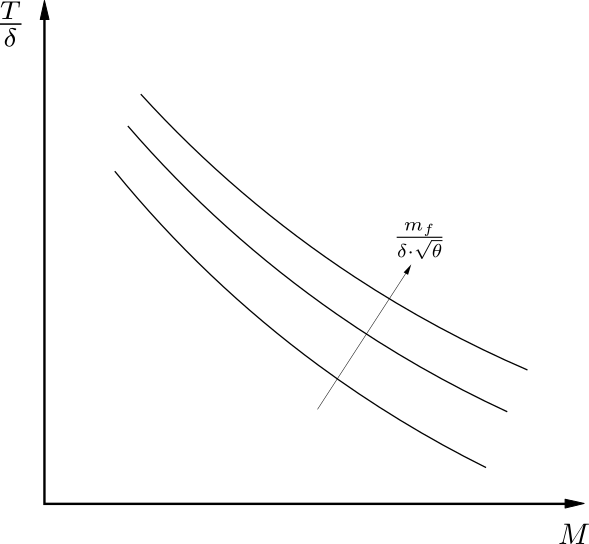
\includegraphics[keepaspectratio, width=0.50\textwidth]{TDelta}
\caption{Qualitative trend of  the generalized thrust v.s. Mach number parameterized in generalized fuel flow rate}
\label{fig:Figure1}
\end{figure}
%
where
%
\begin{itemize}
\item $T$, is the net thust
\item $T_{f}$, is the gross thrust
\item $M$, is the mach number
\item $a_{0}$, is the sound speed at sea level
\item $\dfrac{\sqrt{\theta \cdot m_{a}}}{\delta}$, is the genralized air flow rate which is function of the generalized fuel flow rate given by $\dfrac{m_{f}}{\delta \cdot \sqrt{\theta}}$
\end{itemize}
%
\noindent
In this way that the genralized thrust results as a function of Mach number and generalized fuel flow rate.
%
\begin{equation}
\frac{T}{\delta}=\frac{T_{f}}{\delta}\cdot f\left(\frac{m_{f}}{\delta \cdot \sqrt{\theta}}\right)
\label{eqn:Equation2}
\end{equation}
%
\noindent
As shown in figure~\ref{fig:Figure1} the generalized thrust decreases with Mach number, at given fuel flow rate, and grows with the latter, at given Mach number. This because if the Mach number grows at fixed fuel flow rate, the air flow rate grows reducing the thrust; otherwise, if fuel flow rate grows at fixed Mach number, air flow rate is lower giving more thrust.
%
With this function it's possible to correlate generalized thrust to hourly fuel consumption which is a main keypoint in building the cruise grid chart of an endurance based aircraft such as \gls{acr:UAV}. 
%
Since transport aircrafts rely more on range performance, it's necessary to obtain the same relationship between generalized thurst and fuel consumption referred to the generalized specific range indicated with $\delta\bar s $. 

\bigskip
\noindent
Dividing the generalized fuel flow rate, which is dimesionally equal to $\frac{\si{\kilogram}}{\second}$, by a velocity, the result has a dimension of $\frac{\meter}{\si{\kilogram}}$ that represents the reciprocal of the specific range. In this way it's possible to state the following relation.
%
\begin{equation}
\frac{m_{f}}{\delta \cdot \sqrt{\theta}}=\frac{M\cdot a_{0}}{\delta\bar s}
\label{eqn:Equation3}
\end{equation}
%
\begin{figure}[!ht]
\centering
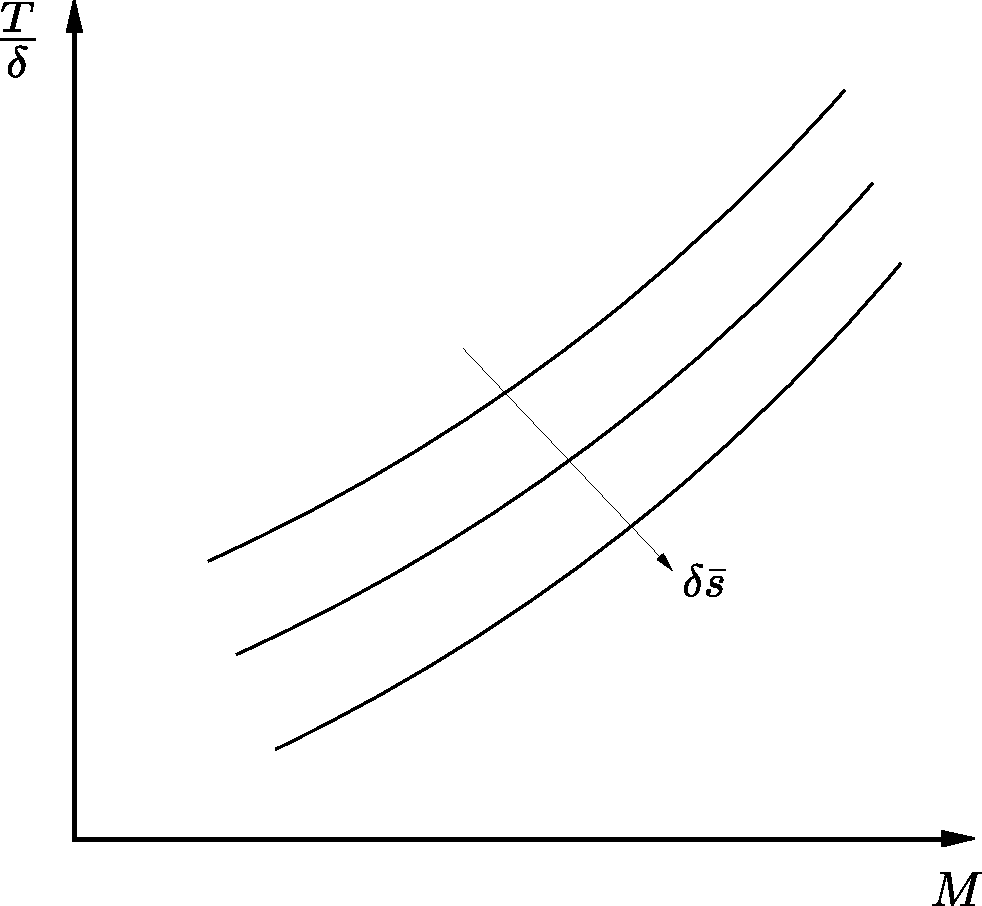
\includegraphics[keepaspectratio, width=0.50\textwidth]{TDelta_SpecificRange}
\caption{Qualitative trend of the generalized thrust v.s. Mach number parameterized in generalized specific range}
\label{fig:Figure2}
\end{figure}
%
\noindent
As expectd from the relation (\ref{eqn:Equation3}) the thrust has a trend which is the inverse of the previous parameterization. In fact now, for a given Mach number, if the pilot wants to go farther he has to decrease the thrust in order to reduce the fuel consumption; otherwise, at a given distance to reach, the pilot has to increase the thrust in order to make the Mach number grows.

\bigskip
\noindent
Since the thrust has always to be compared with the drag in order to evaluate if the aircraft can fly in a specific cruise condition without loosing speed and altitude, it's necessary to obtain a generalized drag trend as well. 
%
This ai very similar to the drag trend, as can be seen from figure~\ref{fig:Figure3}, and it depends from aircraft weight as well; but, since these have to be generalized quantities, the weight is a generalized weight too.
%
\begin{figure}[b]
\centering
\includegraphics[keepaspectratio, width=0.50\textwidth]{DragDelta_SpecificRange}
\caption{Qualitative trend of the generalized drag v.s. Mach number parameterized in generalized weight}
\label{fig:Figure3}
\end{figure}

\bigskip
\noindent
By the overlap of figure~\ref{fig:Figure2} and figure~\ref{fig:Figure3} charts, it's easy to note that the best Mach number, for a given generalized weight, is located at the intersection of the two curves as reported in figure~\ref{fig:Figure4}. In fact, in order to obtain a bigger specific range at fixed weight, the generalized drag would be higher than the generalized thrust; otherwise, if the pilot wants to fly faster at given weight, he has to increase thrust so that the specific range will decrease due to the increasing fuel consumption.
%
Since during the cruise phase the aircraft weight decreases continuously, the pilot has to gain altitude in order to leave the generalized weight unchanged; this explains why during cruise the aircraft continues to climb. 
%
\begin{figure}[t]
\centering
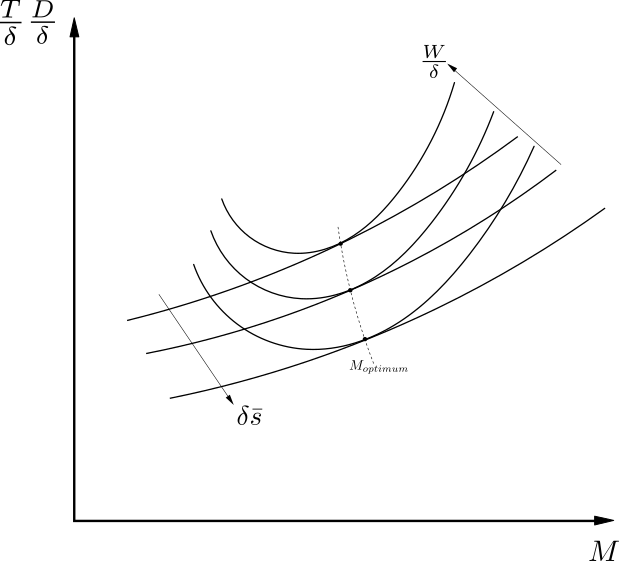
\includegraphics[keepaspectratio, width=0.50\textwidth]{TDeltaDragDelta}
\caption{Comparison between generalized drag and generalized thrust as functions of Mach number}
\label{fig:Figure4}
\end{figure}

\bigskip
\noindent
The specific range can also be connected to Breguet formulas (\ref{eqn:BreguetEquation}) as it can be obtained by dividng the \gls{AF} by the aircraft weight; in particular the autonomy factor, groups three main aircraft efficiency and can be written as follow.
%
\begin{subequations}\label{eqn:AutonomyFactor}
\begin{equation}\label{eqn:AutonomyFactorProp}
A.F.=
      \begin{array}{l@{\rule{5em}{0pt}}l} 
      \dfrac{\eta_{p}}{SFC}\cdot\left(\dfrac{L}{D}\right)
          & \text{if} \;\, \text{propeller engine driven}
      \end{array}
\end{equation}
\begin{equation}\label{eqn:AutonomyFactorJet}
A.F.=
      \begin{array}{l@{\rule{7em}{0pt}}l} 
      \dfrac{V}{SFCJ}\cdot\left(\dfrac{L}{D}\right)
          & \text{if} \;\, \text{jet engine driven}
      \end{array}
\end{equation}
\end{subequations}
%
where
%
\begin{itemize}
\item $\eta_{p}$, is propeller efficiency
\item $SFC$, is related to propulsive efficiency
\item $\left(\frac{L}{D}\right)$, is the aerodynamic efficiency
\end{itemize}
%
\noindent 
At given generalized weight and generalized specific range, the optimum Mach is known as explained before and so the autonomy factor can be calculated by multiply $\frac{W}{\delta}$ and $\delta\bar s$. Repeating this operation for different generalized weight conditions, allows to define the autonomy factor trend as function of the generalized weight in which each point of the chart is related to an optimum Mach number for the specific range.
%
\begin{figure}[t]
\centering
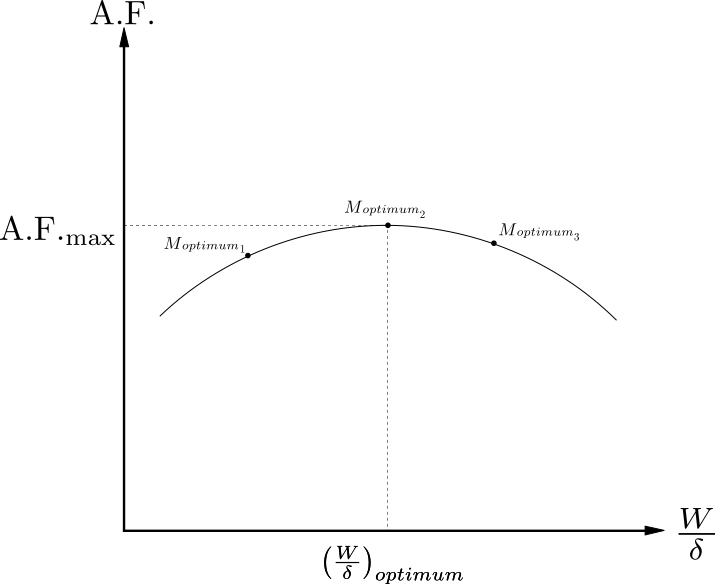
\includegraphics[keepaspectratio, width=0.60\textwidth]{AutonomyFactor}
\caption{Autonomy factor trend as function of the generalized weight}
\label{fig:Figure5}
\end{figure}
%
\noindent
As can be seen from figure~\ref{fig:Figure5} the autonomy factor has a maximum at a specific generalized weight which is the one that the pilot should maintain during the cruise phase. 
%
If the altitude is fixed, and so $\delta$ is constant, the chart in figure~\ref{fig:Figure5} can be seen as function of Mach number for a given aircraft weight; at this point, knowing that the autonomy factor leads to the specific range if divided by the aircraft weight, it's possible to define the specific range trend as funcion of the Mach number parameterized in aircraft weight. 

\bigskip
\noindent
The chart, so obtained, in figure~\ref{fig:Figure6} is the one upon which the cruise grid is defined; on the latter, in fact, four lines are drawn each of which is related to a precise mission objecive.
%
It's important to highlight that, on long distances, the maximum distance line is not often followed during the cruise because it is tied to a low speed which adversely affects the total flight time increasing the D.O.C.; in order to avoid this condition, pilots prefer to follow the long range line which has only 1\% of penalty on the specific range but, at the same time, allows to fly at significantly higher speed with benefits on flight time and, as a result, on the~D.O.C.
%
\begin{figure}[H]
\centering
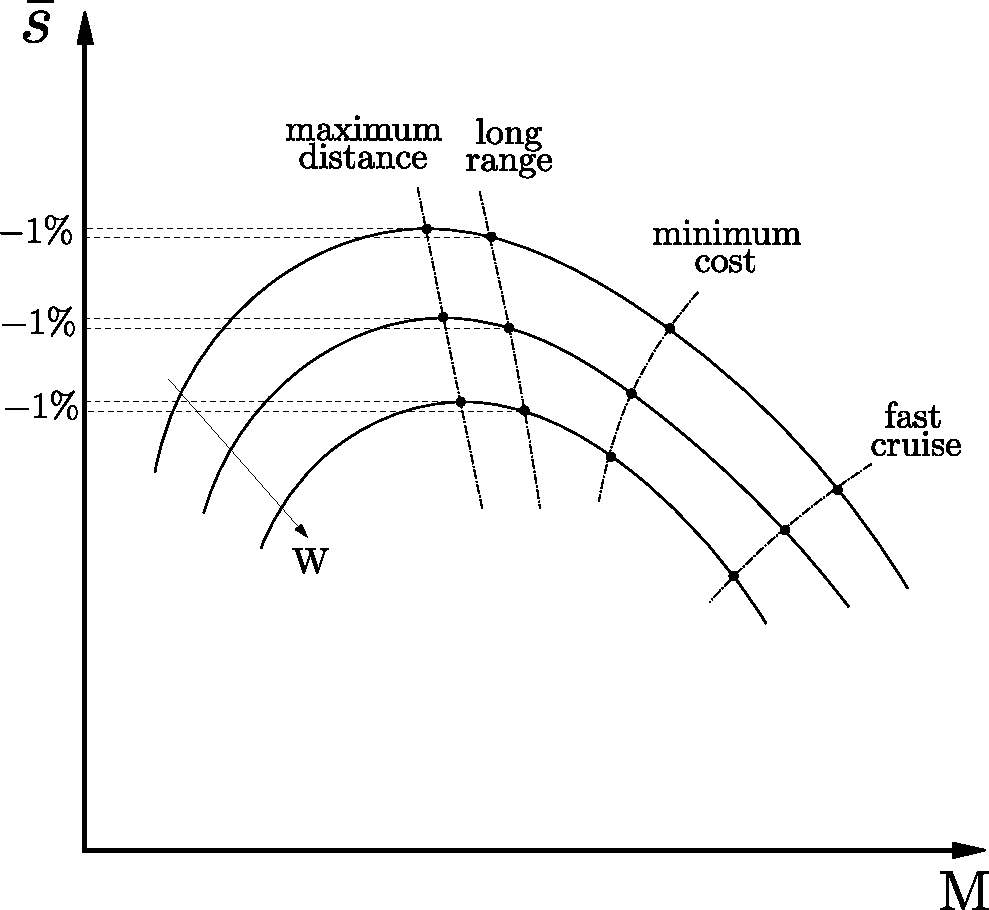
\includegraphics[keepaspectratio, width=0.50\textwidth]{CruiseGrid}
\caption{Specific range as function of the Mach number parameterized in aricraft weight}
\label{fig:Figure6}
\end{figure}
%------------------------- JAVA CLASS ARCHITECTURE ---------------------------
%
\section{Java class architecture}
After having introduced the theory behind the cruise grid chart, a presentation of the related Java class inside JPAD is shown. Using the same philosophy of the previous chapter, a dedicated class, named \lstinline[language=Java]!SpecificRangeCalc!, has been implemented inside which a series of static methods provide the needed calculation tools. Generaly speaking, the giudeline followed in creating this class is to assign an array of Mach numbers, starting from the one realitve to the minimum cruising speed and ending with the maximum cruising speed at that altitude and weight, and then evaluate the $SFC$, from engine database, for each Mach number; from here the $A.F.$ is built after the evaluation of the aerodynamic efficinecy for each value of the same Mach array. Finally the specific range is calculated, in $\frac{\si{nmi}}{\si{lbs}}$, dividing the $A.F.$ by the aircraft max take off mass.

\bigskip
\noindent
The first \gls{Static} presented is \lstinline[language=Java]!calculateEfficiencyVsMach!. It allows to evaluate the aerodynamic efficiency value for each  Mach number of a given array through the evaluation of the $C_{L}$ and the relative $C_{D}$ from the aircraft total drag polar; in particular the two aerodynamic coefficients are calculated by calling other two static methods which come from two classes of the aerodynamic calculator package of \lstinline[language=Java]!JPADCore! named, respectively, \lstinline[language=Java]!LiftCalc! and \lstinline[language=Java]!DragCalc!.
%
The static \lstinline[language=Java]!LiftCalc! method, named \lstinline[language=Java]!calculateLiftCoeff!, performs the $C_{L}$ calculation using the following formula, valid in cruise phase.
%
\begin{equation}
C_L=\frac{2W}{\rho S V^2}
\label{eqn:Lift.Equation}
\end{equation}
%
\noindent
where $V$, is the \gls{TAS} derived from the actual Mach number of the array at that the given altitude.
%
\begin{table}[b]
\begin{tabular}{p{7cm}p{7.5cm}}
\toprule
\lstinline[language=Java]!maxTakeOffMass! & Maximum take-off mass \\[0.1	cm]
\lstinline[language=Java]!sweepHalfChordEquivalent! & Equivalent wing sweep angle at half chord \\[0.1cm]
\lstinline[language=Java]!surface! & Wing surface \\[0.1cm]
\lstinline[language=Java]!cd0!	& Wing c\textsubscript{D0} \\[0.1cm]
\lstinline[language=Java]!oswald!	& Wing oswald factor \\[0.1cm]
\lstinline[language=Java]!mach!	& An array of Mach numbers \\[0.1cm]
\lstinline[language=Java]!ar!	& Wing aspect ratio \\[0.1cm]
\lstinline[language=Java]!tcMax! & Mean maximum thickness of the wing \\[0.1cm]
\lstinline[language=Java]!altitude! & Cruise altitude \\[0.1cm]
\lstinline[language=Java]!airfoilType! & The wing airfoil type from the related \lstinline[language=Java]!AirfoilType! enumeration \\
\bottomrule
\end{tabular}
\caption{ \lstinline[language=Java]!calculateEfficiencyVsMach! input data}
\label{table:Table1}
\end{table}
%
On the other hand, the static \lstinline[language=Java]!DragCalc! method, named \lstinline[language=Java]!calculateCDTotal!, performs the $C_{D}$ calculation using the total drag polar expression.
%
\begin{equation}
C_D=C_{D0}+\frac{C_L^2}{\pi \ensuremath{\AR} e}+C_{D\text{wave}}
\label{eqn:Drag.Total}
\end{equation}
%
\noindent
In particular the $C_{D\text{wave}}$ is calculated as presented in~\cite{hilton1951high}.

\bigskip
\noindent
The second \gls{Static} implemented is \lstinline[language=Java]!calculateSfcVsMach!, which accepts as input data reported in table~\ref{table:Table2} allows to evaluate the $SFC$ of a turboprop aircraft, or the $SFCJ$ of a turbofan aircraft, for each Mach number of the given array by reading data from the related engine database.
%
\begin{table}[t]
\begin{tabular}{p{7cm}p{7.5cm}}
\toprule
\lstinline[language=Java]!mach!	& An array of Mach numbers \\[0.1cm]
\lstinline[language=Java]!altitude! & Cruise altitude \\[0.1cm]
\lstinline[language=Java]!bpr! & Engine By-Pass ratio \\[0.1cm]
\lstinline[language=Java]!engineType! & The engine type from the related \lstinline[language=Java]!EngineType! enumeration \\
\bottomrule
\end{tabular}
\caption{ \lstinline[language=Java]!calculateSfcVsMach! input data}
\label{table:Table2}
\end{table}

\bigskip
\noindent
Finally, the two previous method leads to the last one named \lstinline[language=Java]!calculateSpecificRangeVsMach! which allows to calculate the $A.F.$ and, from it, the specific range by implementing the (\ref{eqn:AutonomyFactorProp}) or the (\ref{eqn:AutonomyFactorJet}) depending on the given engine type. 
%
To do this, it's necessary to give as input the Mach numbers array, the aerodynamic efficiency array calculated with~\lstinline[language=Java]!calculateEfficiencyVsMach! and the $SFC$ array calculated with~\lstinline[language=Java]!calculateSfcVsMach! as shown in table~\ref{table:Table3}.
%
\begin{table}[!b]
\begin{tabular}{p{7cm}p{7.5cm}}
\toprule
\lstinline[language=Java]!maxTakeOffMass! & Maximum take-off mass \\[0.1	cm]
\lstinline[language=Java]!mach!	& An array of Mach numbers \\[0.1cm]
\lstinline[language=Java]!efficiency!	& An array of aerodynamic efficiency values \\[0.1cm]
\lstinline[language=Java]!sfc!	& An array of SFC values \\[0.1cm]
\lstinline[language=Java]!bpr! & Engine By-Pass ratio \\[0.1cm]
\lstinline[language=Java]!altitude! & Cruise altitude \\[0.1cm]
\lstinline[language=Java]!eta!	& Propeller efficiency (set to zero in case of turbofan) \\[0.1cm]
\lstinline[language=Java]!engineType! & The engine type from the related \lstinline[language=Java]!EngineType! enumeration \\
\bottomrule
\end{tabular}
\caption{ \lstinline[language=Java]!calculateSpecificRangeVsMach! input data}
\label{table:Table3}
\end{table}

\bigskip
\noindent
The class is completed by other four static methods demanded of plotting the results; in particular, using the same approach shown in the previous chapter, a .png and a .tikz output images are created for each of the $SFC$, the aerodynamic efficiency and the specific range.
%
It's important to highlight that the first of these plotting methods, which is named \lstinline[language=Java]!createSpecificRangeChart! and is demanded of plotting the cruise grid chart, has implemented, inside it, the evaluation of the maximum range condition as well as the long range one; this by calculating all maximum points and, from them, all points at -1\% of penalty obtained through the evaluation of the bigger of the two intersction points that the line at -1\% of penalty defines on each specific range curve.
%
\noindent
The fourth method is, insetad, used for plotting the intersection between the required and available thrust, giving as input a speed array, the altitude and two \gls{List} of custom \gls{Map} named~\lstinline[language=Java]!DragMap! and~\lstinline[language=Java]!ThustMap!; these are two classes used to store all data related to drag and thrust curves like the aircraft weight, the current altitude, the speed array on which the drag or thrust are evaluated and, finally, the drag or thrust array itself.  

\bigskip
\noindent
In conclusion a flowchart of the described class is shown in figure~\ref{fig:Figure7} in order to simplify its understanding.
%
\begin{figure}[t]
\centering
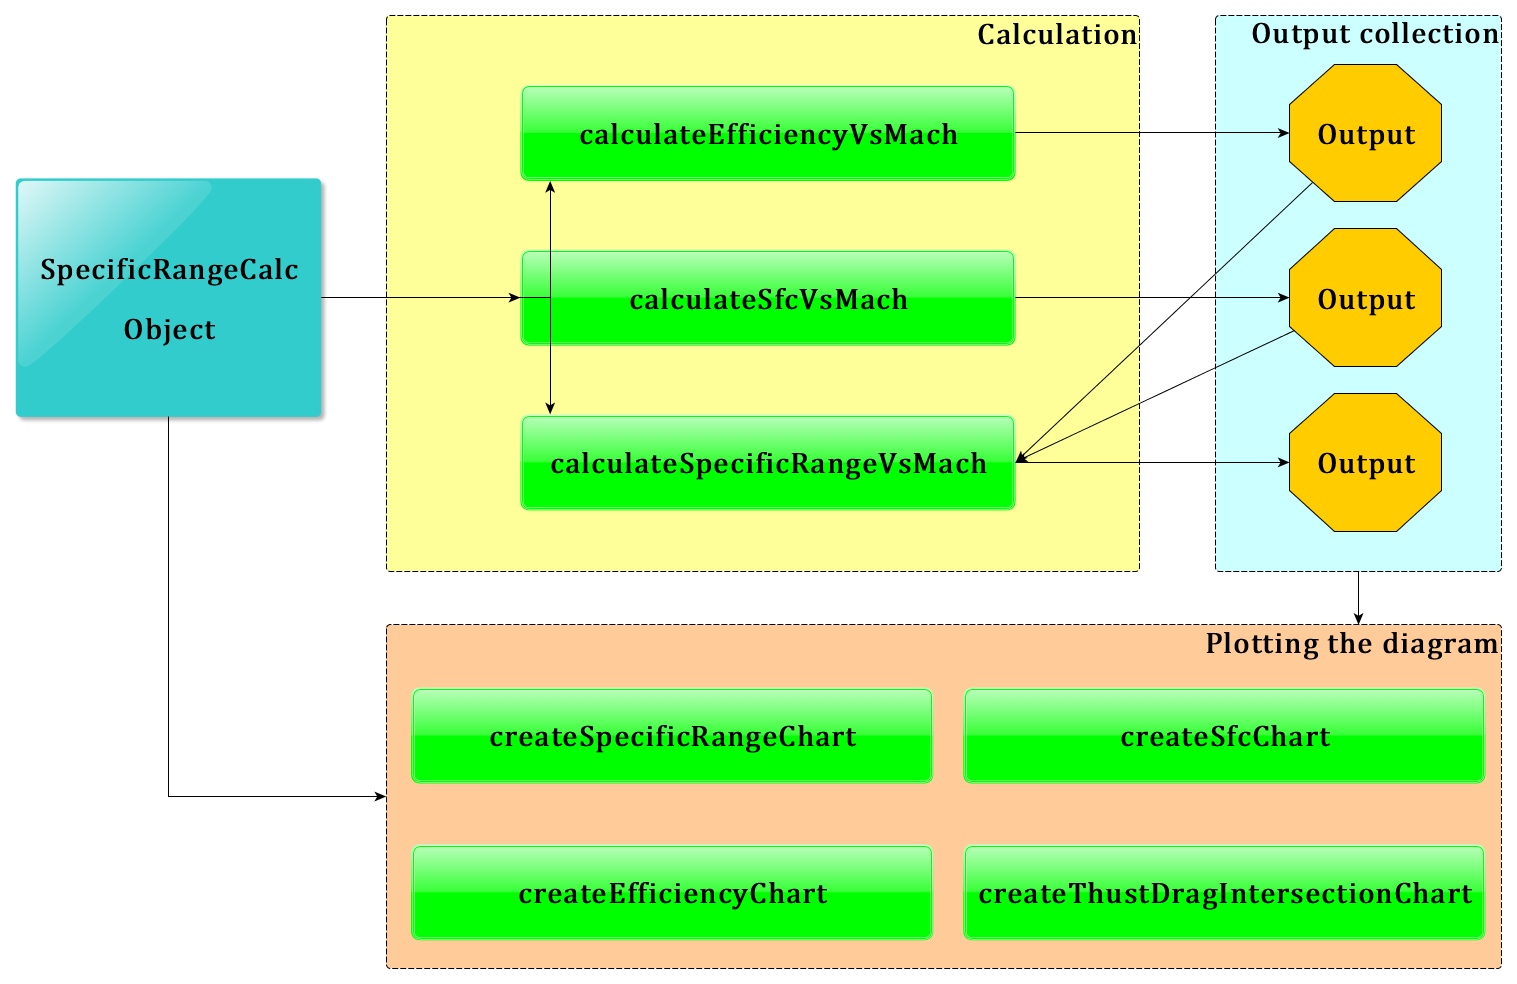
\includegraphics[keepaspectratio, width=0.90\textwidth]{SpecificRange_Flowchart}
\caption{\lstinline[language=Java]!SpecificRangeCalc! class flowchart}
\label{fig:Figure7}
\end{figure}
%
%----------------------- CASE STUDY : ATR72 AND B747 -------------------------
\section{Case study: ATR-72 and B747-100B}
%
In order to validate all the teoretical concepts explained in the previous paragraphs, as well as to give to the reader a useful example of how to handle this class usage, the following pages shows two application of the class methods made upon the two default aircraft described in paragraph~\ref{par:DefaultAircraft}.

\bigskip
\noindent
Once all preliminary steps have been completed, as explained in paragraph~\ref{par:DefaultAircraft}, it's possible to start the test of this class. 
%
First of all, since the cruise grid chart is parameterized in aircraft weight, an array of aircraft masses has to be created; in particular, in this test, a variation of mass of -10\% has been implemented, starting from the aircraft maximum take-off mass until it reaches the 60\% of the latter. 
%
The second step is to define the independent variable, which is the Mach number, and in particular it's necessary to identify the upper and lower limitations of its array; this can be done by evaluating the required thrust, which is equal to the drag during cruise, and comparing it with the available thrust supplied by the power plant.
%
\noindent
By the intersections of the latter, the two required speeds can be derived; otherwise, if the minimum speed intersection can't be found, the cruising stalling speed, at that weight and altitude condition and for a specified $C_{L\text{max}}$, replaces the missing intersection abscissa.
%
\begin{figure}[t]
\begin{lstlisting}[caption={Mass variation in Specific Range test - B747-100B}, captionpos=b, tabsize=2]
		double[] maxTakeOffMassArray = new double[5];
		for (int i=0; i<5; i++)
			maxTakeOffMassArray[i] =	aircraft.get_weights().get_MTOM()
							.plus(aircraft.get_weights().get_MLM())
							.divide(2)
							.getEstimatedValue()
							*(1-0.1*(4-i));

		double[] weight = new double[maxTakeOffMassArray.length];
		for(int i=0; i<weight.length; i++)
			weight[i] = maxTakeOffMassArray[i]*AtmosphereCalc.g0.getEstimatedValue();
\end{lstlisting}
\end{figure}
%
In terms of code, the last step can be carried out using the static method, of the \lstinline[language=Java]!JPADCore! class~\lstinline[language=Java]!PerformanceCalcUtils!, named~\lstinline[language=Java]!calculateDragThrustIntersection!; the latter requires as input the following data:
%
\begin{itemize}
\item An array of altitudes
\item An array of speeds
\item An array of weights
\item An array of throttle settings
\item An array of flight conditions chosen from the \lstinline[language=Java]!EngineOperatingConditionEnum! enumeration
\item The engine by-pass ratio, set to zero in case of propeller aircraft
\item The wing surface
\item Wing C\textsubscript{Lmax} in clean configuration
\item A~\lstinline[language=Java]!List! of custom data map named~\lstinline[language=Java]!DragMap!
\item A~\lstinline[language=Java]!List! of custom data map named~\lstinline[language=Java]!ThrustMap!
\end{itemize}

\bigskip
\noindent
The last two input are two collections of maps designed to store all data necessary to manage curves of drag, or thrust, as function of speed; in particular, in the reported example, the drag and thrust arrays passed to each of them are calculated using the static method of the~\lstinline[language=Java]!JPADCore! classes~\lstinline[language=Java]!DragCalc! and~\lstinline[language=Java]!ThrustCalc! named, respectively,~\lstinline[language=Java]!calculateDragVsSpeed! and~\lstinline[language=Java]!calculateThrustVsSpeed!. 
%
The first one implements the classic formula of drag as function of speed and of the $C_{D}$ calculated with the (\ref{eqn:Drag.Total}), while the second one recognizes the engine type and reads the thrust value from the related external database.

\bigskip
\begin{lstlisting}[caption={Intersection of drag and thrust curves in Specific Range test - B747-100B}, captionpos=b, tabsize=2]
		// Drag Thrust Intersection		
		double[] speed = MyArrayUtils.linspace(
				SpeedCalc.calculateTAS(
						0.05,
						theCondition.get_altitude().getEstimatedValue()
						), // start
				SpeedCalc.calculateTAS(
						1.0,
						theCondition.get_altitude().getEstimatedValue()
						), // ending
				250 // points
				);

		List<DragMap> listDrag = new ArrayList<DragMap>();
		for(int i=0; i<maxTakeOffMassArray.length; i++)
			listDrag.add(
					new DragMap(
							weight[i],
							theCondition.get_altitude().getEstimatedValue(),
							DragCalc.calculateDragVsSpeed(
									weight[i],
									theCondition.get_altitude().getEstimatedValue(),
									aircraft.get_wing().get_surface().getEstimatedValue(),
									aircraft.get_theAerodynamics().get_cD0(),
									aircraft.get_wing().get_aspectRatio(),
									aircraft.get_theAerodynamics().get_oswald(),
									speed,
									aircraft.get_wing().get_sweepHalfChordEq().getEstimatedValue(),
									aircraft.get_wing().get_maxThicknessMean(),
									AirfoilTypeEnum.MODERN_SUPERCRITICAL
									),
							speed
							)
					);

		List<ThrustMap> listThrust = new ArrayList<ThrustMap>();
		for(int i=0; i<maxTakeOffMassArray.length; i++)
			listThrust.add(
					new ThrustMap(
							theCondition.get_altitude().getEstimatedValue(),
							1.0, // phi
							ThrustCalc.calculateThrustVsSpeed(
									aircraft.get_powerPlant()
													.get_engineList().get(0).get_t0().getEstimatedValue(),
									1.0, // phi
									theCondition.get_altitude().getEstimatedValue(),
									EngineOperatingConditionEnum.CRUISE,
									EngineTypeEnum.TURBOFAN,
									aircraft.get_powerPlant().get_engineList().get(0).get_bpr(),
									aircraft.get_powerPlant().get_engineNumber(),
									speed
									),
							speed,
							aircraft.get_powerPlant().get_engineList().get(0).get_bpr(),
							EngineOperatingConditionEnum.CRUISE
							)
					);

		List<DragThrustIntersectionMap> intersectionList = PerformanceCalcUtils
				.calculateDragThrustIntersection(
						new double[] {theCondition.get_altitude().getEstimatedValue()},
						speed,
						weight,
						new double[] {1.0},
						new EngineOperatingConditionEnum[] 
										{EngineOperatingConditionEnum.CRUISE},
						aircraft.get_powerPlant().get_engineList().get(0).get_bpr(),
						aircraft.get_wing().get_surface().getEstimatedValue(),
						cLmax,
						listDrag,
						listThrust
						);
		// Definition of a Mach array for each maxTakeOffMass
		List<Double[]> machList = new ArrayList<Double[]>();
		for(int i=0; i<maxTakeOffMassArray.length; i++) 
			machList.add(MyArrayUtils.linspaceDouble(
					intersectionList.get(i).getMinMach(), // start
					intersectionList.get(i).getMaxMach(), // ending
					250)); // points
\end{lstlisting}

\bigskip
\noindent
At this point all static methods of the \lstinline[language=Java]!SpecificRangeCalc! class are called in order to follow the flowchart steps of figure~\ref{fig:Figure7} with the purpose of calculating and plotting the cruise grid points.

\bigskip
\begin{lstlisting}[caption={Intersection of drag and thrust curves in Specific Range test - B747-100B}, captionpos=b, tabsize=2]
		// Calculation of the SFC for each Mach array
		List<Double[]> sfcList = new ArrayList<Double[]>();
		for(int i=0; i<maxTakeOffMassArray.length; i++)
			sfcList.add(SpecificRangeCalc.calculateSfcVsMach(
					machList.get(i),
					theCondition.get_altitude().getEstimatedValue(),
					aircraft.get_powerPlant().get_engineList().get(0).get_bpr(),
					EngineTypeEnum.TURBOFAN
					));
		// Calculation of the Efficiency for each Mach array
		List<Double[]> efficiencyList = new ArrayList<Double[]>();
		for(int i=0; i<maxTakeOffMassArray.length; i++)
			efficiencyList.add(SpecificRangeCalc.calculateEfficiencyVsMach(
					Amount.valueOf(maxTakeOffMassArray[i],SI.KILOGRAM),
					machList.get(i),
					aircraft.get_wing().get_surface().getEstimatedValue(),
					theCondition.get_altitude().getEstimatedValue(),
					aircraft.get_wing().get_aspectRatio(),
					aircraft.get_theAerodynamics().get_oswald(),
					aircraft.get_theAerodynamics().get_cD0(),
					aircraft.get_wing().get_maxThicknessMean(),
					aircraft.get_wing().get_sweepHalfChordEq(),
					AirfoilTypeEnum.MODERN_SUPERCRITICAL));
		// Calculation of the Specific range:
		List<Double[]> specificRange = new ArrayList<Double[]>();
		for (int i=0; i<maxTakeOffMassArray.length; i++)
			specificRange.add(SpecificRangeCalc.calculateSpecificRangeVsMach(
					Amount.valueOf(maxTakeOffMassArray[i], SI.KILOGRAM),
					machList.get(i),
					sfcList.get(i),
					efficiencyList.get(i),
					theCondition.get_altitude().getEstimatedValue(),
					aircraft.get_powerPlant().get_engineList().get(0).get_bpr(),
					0.85,
					EngineTypeEnum.TURBOFAN));
	
		// PLOTTING:			
		// building legend
		List<String> legend = new ArrayList<String>();
		for(int i=0; i<maxTakeOffMassArray.length; i++)
			legend.add("MTOM = " + maxTakeOffMassArray[i] + " kg ");
		
		SpecificRangeCalc.createSpecificRangeChart(specificRange, machList, legend);
		SpecificRangeCalc.createSfcChart(sfcList, machList, legend, EngineTypeEnum.TURBOFAN);
		SpecificRangeCalc.createEfficiencyChart(efficiencyList, machList, legend);
		SpecificRangeCalc.createThrustDragIntersectionChart(
						theCondition.get_altitude().getEstimatedValue(),
						maxTakeOffMassArray,
						listDrag,
						listThrust,
						speed
						);	
	}
	// END OF THE TEST
\end{lstlisting}

\bigskip
\noindent
In conclusion, the following images shows the cruise grid, and all the evaluated quatities, calculated with this class and referred to the ATR-72 and of the B747-100B. 
%
It's has to be noted that, as explained in the first paragraph, the maximum range condition is actually related to a low speed and also that, with a penalty of -1\% in range, the specific range is about the same with a significantly higher speed; for example, in figure~\ref{fig:SpecificRangeB747}, the cruising Mach number, related to the maximum range condition of the B747-100B, varies, with the aircraft weight, between 0.74 and 0.80 while the long range one varies between 0.80 and 0.82, being more similar to the real cruising Mach number.
%
Moreover, the specific fuel consumption, from figures~\ref{fig:sfcATR} and~\ref{fig:sfcB747}, grows with the Mach number, as expected, due to the major thrust given by engines; while the efficiency, from figures~\ref{fig:EfficiencyATR} and~\ref{fig:EfficiencyB747}, decreases rapidly in the B747-100B case due to the increasing wave drag, not present in the ATR-72 case.
%
\begin{figure}[t]
\centering
%DragThrust
\begin{tikzpicture}

\begin{axis}[
width=\textwidth,
height=0.65\textwidth,
scaled ticks=false, tick label style={/pgf/number format/fixed},
xmin=0.075,
xmax=0.5,
xlabel={Mach },
xmajorgrids,
ymin=7.5E03,
ymax=3.0E04,
ylabel={Drag, Thrust (\newton)},
ymajorgrids,
legend entries = {$\SI{13146}{\kilogram}$\\$\SI{15337}{\kilogram}$\\$\SI{17528}{\kilogram}$\\$\SI{19719}{\kilogram}$\\$\SI{21910}{\kilogram}$\\Thrust\\}
]

\addplot [
color=black,
densely dotted
]
table[row sep=crcr]{
0.07289156626506024	95033.44926153986\\
0.07670682730923695	70123.20781726378\\
0.08052208835341365	54967.940496567404\\
0.08433734939759037	45439.72123741583\\
0.08815261044176707	39178.61592676655\\
0.09196787148594378	34828.70328197726\\
0.09578313253012048	31610.165398884772\\
0.09959839357429719	29076.008451469654\\
0.10341365461847389	26972.077480418586\\
0.10722891566265061	25155.77158791055\\
0.11104417670682733	23548.56103508014\\
0.11485943775100405	22108.167357026385\\
0.11867469879518076	20811.015735521356\\
0.12248995983935748	19639.708534341124\\
0.1263052208835342	18579.476252546\\
0.13012048192771092	17617.682424270624\\
0.13393574297188765	16743.46435245787\\
0.13775100401606435	15947.44250696207\\
0.14156626506024106	15221.483988320875\\
0.1453815261044178	14558.508859711088\\
0.1491967871485945	13952.330692617383\\
0.15301204819277123	13397.524588879505\\
0.15682730923694793	12889.317398405808\\
0.16064257028112466	12423.49596677257\\
0.16445783132530137	11996.330106311983\\
0.1682730923694781	11604.507651111631\\
0.1720883534136548	11245.07947702516\\
0.17590361445783154	10915.412776802988\\
0.17971887550200824	10613.15120358355\\
0.18353413654618497	10336.18075266472\\
0.18734939759036168	10082.600456432036\\
0.1911646586345384	9850.697131791618\\
0.1949799196787151	9638.923552068774\\
0.19879518072289185	9445.879522746\\
0.20261044176706855	9270.295427796513\\
0.20642570281124528	9111.017884754516\\
0.210240963855422	8966.997205214991\\
0.21405622489959872	8837.276405666653\\
0.21787148594377542	8720.981553406113\\
0.22168674698795215	8617.313265328643\\
0.22550200803212886	8525.53920489582\\
0.2293172690763056	8444.987445547711\\
0.2331325301204823	8375.040588067815\\
0.23694779116465903	8315.130535576773\\
0.24076305220883573	8264.733843457405\\
0.24457831325301246	8223.367573031735\\
0.24839357429718917	8190.5855875730185\\
0.2522088353413659	8165.975237533288\\
0.2560240963855426	8149.154388937054\\
0.2598393574297193	8139.768754931535\\
0.26365461847389604	8137.489495656338\\
0.2674698795180728	8142.011056035061\\
0.27128514056224945	8153.049214911639\\
0.2751004016064262	8170.339322247781\\
0.2789156626506029	8193.634703944635\\
0.28273092369477965	8222.705216316672\\
0.2865461847389563	8257.335934384906\\
0.29036144578313305	8297.325960016351\\
0.2941767068273098	8342.48733755693\\
0.2979919678714865	8392.644066019126\\
0.3018072289156632	8447.631198122255\\
0.3056224899598399	8507.294017566353\\
0.30943775100401666	8571.487286871134\\
0.3132530120481934	8640.074558946822\\
0.31706827309237007	8712.92754629922\\
0.3208835341365468	8789.925542419896\\
0.32469879518072353	8870.954890485173\\
0.32851405622490026	8955.908494994364\\
0.33232931726907694	9044.685372426471\\
0.3361445783132537	9137.190237392762\\
0.3399598393574304	9233.333121116548\\
0.34377510040160714	9333.029019385976\\
0.3475903614457838	9436.197567406263\\
0.35140562248996055	9542.762739227739\\
0.3552208835341373	9652.652569649508\\
0.359036144578314	9765.798896698361\\
0.3628514056224907	9882.137122961327\\
0.3666666666666674	10001.605994210775\\
0.37048192771084415	10124.147393904777\\
0.3742971887550208	10249.706152274917\\
0.37811244979919756	10378.229868829934\\
0.3819277108433743	10509.668747208558\\
0.385742971887551	10643.975441409211\\
0.3895582329317277	10781.104912509667\\
0.39337349397590443	10921.014295066665\\
0.39718875502008116	11063.662772455293\\
0.4010040160642579	11209.011460470918\\
0.40481927710843457	11357.023298573684\\
0.40863453815261125	11507.662948207408\\
0.412449799196788	11660.896697671811\\
0.4162650602409647	11816.692373069794\\
0.42008032128514144	11975.019254890358\\
0.4238955823293181	12135.84799982326\\
0.42771084337349485	12299.150567433726\\
0.4315261044176716	12464.900151354963\\
0.4353413654618483	12633.071114683216\\
0.439156626506025	12803.638929284458\\
0.4429718875502017	12976.580118744434\\
0.44678714859437846	13151.872204714213\\
0.4506024096385552	13329.49365642225\\
0.45441767068273187	13509.423843141107\\
0.4582329317269086	13691.642989412963\\
0.46204819277108533	13876.132132852335\\
0.465863453815262	14062.873084357894\\
0.46967871485943874	14251.84839057748\\
0.47349397590361547	14443.041298481608\\
0.4773092369477922	14636.435721911263\\
0.4811244979919689	14832.01620997513\\
0.4849397590361456	15029.767917180403\\
0.48875502008032234	15229.676575189318\\
0.4925702811244991	15431.728466101045\\
0.49638554216867575	15635.910397165524\\
0.5002008032128525	15842.209676842192\\
0.5040160642570292	16050.614092122516\\
0.5078313253012059	16261.11188704056\\
0.5116465863453826	16473.691742301125\\
0.5154618473895594	16688.34275595939\\
0.5192771084337361	16905.05442509055\\
0.5230923694779128	17123.81662839193\\
0.5269076305220896	17344.61960966367\\
0.5307228915662663	17567.453962117695\\
0.5345381526104429	17792.310613467842\\
0.5383534136546196	18019.180811757004\\
0.5421686746987964	18248.05611187992\\
0.5459839357429731	18478.92836276295\\
0.5497991967871498	18711.789695164327\\
0.5536144578313266	18946.632510060994\\
0.5574297188755033	19183.449467589868\\
0.56124497991968	19422.23347651355\\
0.5650602409638567	19662.97768418221\\
0.5688755020080334	19905.675466965185\\
0.5726907630522101	20150.32042112724\\
0.5765060240963868	20396.90635412614\\
0.5803212851405636	20645.42727630932\\
0.5841365461847403	20895.877392989045\\
0.587951807228917	21148.25109687621\\
0.5917670682730937	21402.542960854687\\
0.5955823293172704	21658.747825672\\
0.5993975903614471	21916.87083282955\\
0.6032128514056239	22176.963032725394\\
0.6070281124498006	22439.13798163384\\
0.6108433734939773	22703.57644621452\\
0.6146586345381541	22970.53098335575\\
0.6184738955823308	23240.330611593414\\
0.6222891566265074	23513.38557400712\\
0.6261044176706841	23790.192192500625\\
0.6299196787148609	24071.337813378323\\
0.6337349397590376	24357.50584413446\\
0.6375502008032143	24649.480881375875\\
0.6413654618473911	24948.15392980323\\
0.6451807228915678	25254.52771217973\\
0.6489959839357445	25569.7220702198\\
0.6528112449799212	25894.97945633377\\
0.6566265060240979	26231.670516167836\\
0.6604417670682746	26581.29976188161\\
0.6642570281124514	26945.511336108775\\
0.6680722891566281	27326.094866548458\\
0.6718875502008048	27724.99141113844\\
0.6757028112449815	28144.299493762966\\
0.6795180722891583	28586.281230450724\\
0.6833333333333349	29053.36854602061\\
0.6871485943775116	29548.169481135057\\
0.6909638554216884	30073.47458972242\\
0.6947791164658651	30632.26342673229\\
0.6985943775100418	31227.711126188755\\
0.7024096385542186	31863.195069508845\\
0.7062248995983953	32542.30164405459\\
0.7100401606425719	33268.83309188891\\
0.7138554216867486	34046.81444870671\\
0.7176706827309254	34880.50057291422\\
0.7214859437751021	35774.383264830634\\
0.7253012048192788	36733.198475987374\\
0.7291164658634556	37761.933608501575\\
0.7329317269076323	38865.83490450147\\
0.736746987951809	40050.41492558215\\
0.7405622489959857	41321.46012227132\\
0.7443775100401624	42685.03849348624\\
0.7481927710843391	44147.50733596206\\
0.7520080321285159	45715.52108363527\\
0.7558232931726926	47396.03923696447\\
0.7596385542168693	49196.33438217248\\
0.763453815261046	51124.000300394924\\
0.7672690763052228	53186.960166719735\\
0.7710843373493994	55393.47483910411\\
0.7748995983935761	57752.15123715574\\
0.7787148594377529	60271.95081076438\\
0.7825301204819296	62962.19809857296\\
0.7863453815261063	65832.58937627527\\
0.7901606425702831	68893.20139472971\\
0.7939759036144598	72154.50020787829\\
0.7977911646586364	75627.35009046018\\
0.8016064257028132	79323.02254551115\\
0.8054216867469899	83253.2054016374\\
0.8092369477911666	87430.012000057\\
0.8130522088353432	91865.99047139949\\
0.8168674698795199	96574.13310225484\\
0.8206827309236965	101567.8857914649\\
0.8244979919678731	106861.15759614855\\
0.8283132530120497	112468.33036745459\\
0.8321285140562263	118404.26847603486\\
0.8359437751004031	124684.32862723032\\
0.8397590361445797	131324.3697659651\\
0.8435742971887563	138340.76307134127\\
0.8473895582329329	145750.40204092945\\
0.8512048192771096	153570.71266474726\\
0.8550200803212862	161819.66368892443\\
0.8588353413654628	170515.7769690452\\
0.8626506024096394	179678.13791316544\\
0.866465863453816	189326.40601449963\\
0.8702811244979927	199480.8254737713\\
0.8740963855421693	210162.23591122584\\
0.8779116465863459	221392.08316829707\\
0.8817269076305225	233192.43019892828\\
0.8855421686746991	245585.96805053993\\
0.8893574297188758	258596.0269346431\\
0.8931726907630524	272246.58738709294\\
0.8969879518072291	286562.2915179806\\
0.9008032128514057	301568.4543511567\\
0.9046184738955824	317291.0752533921\\
0.908433734939759	333756.84945315844\\
0.9122489959839356	350993.179649041\\
0.9160642570281122	369028.18770776823\\
0.9198795180722888	387890.7264518651\\
0.9236947791164655	407610.3915369216\\
0.9275100401606421	428217.5334184736\\
0.9313253012048187	449743.26940850064\\
0.9351405622489953	472219.49582152796\\
0.938955823293172	495678.90021033975\\
0.9427710843373486	520154.9736912967\\
0.9465863453815252	545682.0233592567\\
0.9504016064257018	572295.1847920951\\
0.9542168674698784	600030.4346448283\\
0.9580321285140552	628924.6033333297\\
0.9618473895582318	659015.3878076443\\
0.9656626506024084	690341.3644149007\\
0.969477911646585	722942.0018518058\\
0.9732931726907617	756857.6742067413\\
0.9771084337349383	792129.6740914409\\
0.9809236947791149	828800.22586226\\
0.9847389558232915	866912.4989310282\\
0.9885542168674681	906510.6211654935\\
0.9923694779116448	947639.6923793383\\
0.9961847389558214	990345.7979117925\\
1.0	1034676.0222968363\\
};

\addplot [
color=black,
dashed
]
table[row sep=crcr]{
0.07289156626506024	192357.4790767701\\
0.07670682730923695	133799.26493196047\\
0.08052208835341365	97876.91141201754\\
0.08433734939759037	75437.44472610267\\
0.08815261044176707	61093.63920443415\\
0.09196787148594378	51643.09242890667\\
0.09578313253012048	45168.724671473305\\
0.09959839357429719	40518.128107108925\\
0.10341365461847389	36997.726160069215\\
0.10722891566265061	34190.865976273126\\
0.11104417670682733	31848.513293406355\\
0.11485943775100405	29823.048405828406\\
0.11867469879518076	28027.942927398046\\
0.12248995983935748	26413.126112610367\\
0.1263052208835342	24949.867296408276\\
0.13012048192771092	23619.977908440134\\
0.13393574297188765	22408.67046675765\\
0.13775100401606435	21303.17838866254\\
0.14156626506024106	20292.431894331065\\
0.1453815261044178	19366.7944030872\\
0.1491967871485945	18517.845498340634\\
0.15301204819277123	17738.201290928802\\
0.15682730923694793	17021.364993226976\\
0.16064257028112466	16361.602033936186\\
0.16445783132530137	15753.835213175254\\
0.1682730923694781	15193.556305118947\\
0.1720883534136548	14676.751224123616\\
0.17590361445783154	14199.83642698844\\
0.17971887550200824	13759.604663818513\\
0.18353413654618497	13353.178539324836\\
0.18734939759036168	12977.970625365486\\
0.1911646586345384	12631.64908939603\\
0.1949799196787151	12312.107983998136\\
0.19879518072289185	12017.441488856308\\
0.20261044176706855	11745.921515489646\\
0.20642570281124528	11495.978182208595\\
0.210240963855422	11266.182746461878\\
0.21405622489959872	11055.23264735914\\
0.21787148594377542	10861.938365387434\\
0.22168674698795215	10685.211851320877\\
0.22550200803212886	10524.056313759947\\
0.2293172690763056	10377.557185998077\\
0.2331325301204823	10244.87411910169\\
0.23694779116465903	10125.233870096099\\
0.24076305220883573	10017.923972696819\\
0.24457831325301246	9922.287093703266\\
0.24839357429718917	9837.715991459587\\
0.2522088353413659	9763.649004081064\\
0.2560240963855426	9699.56600476771\\
0.2598393574297193	9644.984769747694\\
0.26365461847389604	9599.457711433251\\
0.2674698795180728	9562.56893541484\\
0.27128514056224945	9533.931585118926\\
0.2751004016064262	9513.185442437834\\
0.2789156626506029	9499.994756514792\\
0.28273092369477965	9494.04627622228\\
0.2865461847389563	9495.047464783338\\
0.29036144578313305	9502.724877516963\\
0.2941767068273098	9516.82268589399\\
0.2979919678714865	9537.101333014747\\
0.3018072289156632	9563.336307302745\\
0.3056224899598399	9595.317022683035\\
0.30943775100401666	9632.845794807445\\
0.3132530120481934	9675.73690402601\\
0.31706827309237007	9723.815736804954\\
0.3208835341365468	9776.917998174473\\
0.32469879518072353	9834.888988569002\\
0.32851405622490026	9897.582939112612\\
0.33232931726907694	9964.862400012822\\
0.3361445783132537	10036.597677268315\\
0.3399598393574304	10112.666313377482\\
0.34377510040160714	10192.952608163076\\
0.3475903614457838	10277.347176209978\\
0.35140562248996055	10365.746537753357\\
0.3552208835341373	10458.052740158666\\
0.359036144578314	10554.17300740681\\
0.3628514056224907	10654.019415241246\\
0.3666666666666674	10757.508589852141\\
0.37048192771084415	10864.561428168541\\
0.3742971887550208	10975.102838005656\\
0.37811244979919756	11089.061496472605\\
0.3819277108433743	11206.369625188765\\
0.385742971887551	11326.962780985328\\
0.3895582329317277	11450.779660884817\\
0.39337349397590443	11577.761920256124\\
0.39718875502008116	11707.854003137569\\
0.4010040160642579	11841.002983806175\\
0.40481927710843457	11977.15841874936\\
0.40863453815261125	12116.272208265653\\
0.412449799196788	12258.298466985232\\
0.4162650602409647	12403.193402659268\\
0.42008032128514144	12550.91520262001\\
0.4238955823293181	12701.423927361853\\
0.42771084337349485	12854.681410737458\\
0.4315261044176716	13010.651166303145\\
0.4353413654618483	13169.29829938435\\
0.439156626506025	13330.589424465317\\
0.4429718875502017	13494.492587537756\\
0.44678714859437846	13660.97719307118\\
0.4506024096385552	13830.013935293198\\
0.45441767068273187	14001.574733491476\\
0.4582329317269086	14175.63267107064\\
0.46204819277108533	14352.161938117117\\
0.465863453815262	14531.137777242982\\
0.46967871485943874	14712.536432496692\\
0.47349397590361547	14896.335101143672\\
0.4773092369477922	15082.511888134144\\
0.4811244979919689	15271.04576308826\\
0.4849397590361456	15461.91651964082\\
0.48875502008032234	15655.104736998754\\
0.4925702811244991	15850.591743574825\\
0.49638554216867575	16048.359582570329\\
0.5002008032128525	16248.390979388398\\
0.5040160642570292	16450.66931076741\\
0.5078313253012059	16655.17857553152\\
0.5116465863453826	16861.903366862254\\
0.5154618473895594	17070.82884600138\\
0.5192771084337361	17281.940717301255\\
0.5230923694779128	17495.22520454435\\
0.5269076305220896	17710.669028458622\\
0.5307228915662663	17928.25938536031\\
0.5345381526104429	18147.983926859913\\
0.5383534136546196	18369.83074057137\\
0.5421686746987964	18593.788331768086\\
0.5459839357429731	18819.845605933133\\
0.5497991967871498	19047.991852154133\\
0.5536144578313266	19278.216727316365\\
0.5574297188755033	19510.510241050622\\
0.56124497991968	19744.8627413949\\
0.5650602409638567	19981.264901131362\\
0.5688755020080334	20219.707704762728\\
0.5726907630522101	20460.182436093815\\
0.5765060240963868	20702.680666386575\\
0.5803212851405636	20947.19424305837\\
0.5841365461847403	21193.715278895303\\
0.587951807228917	21442.236141753903\\
0.5917670682730937	21692.749462890675\\
0.5955823293172704	21945.2544867434\\
0.5993975903614471	22199.789116954573\\
0.6032128514056239	22456.449492407475\\
0.6070281124498006	22715.394888352905\\
0.6108433734939773	22976.852188746107\\
0.6146586345381541	23241.120450933322\\
0.6184738955823308	23508.575562552982\\
0.6222891566265074	23779.674990523887\\
0.6261044176706841	24054.96262199905\\
0.6299196787148609	24335.073697170435\\
0.6337349397590376	24620.73983381581\\
0.6375502008032143	24912.794143484396\\
0.6413654618473911	25212.17643922344\\
0.6451807228915678	25519.938534752757\\
0.6489959839357445	25837.24963499918\\
0.6528112449799212	26165.401817907088\\
0.6566265060240979	26505.815607445627\\
0.6604417670682746	26860.04563773716\\
0.6642570281124514	27229.786408235213\\
0.6680722891566281	27616.87812988385\\
0.6718875502008048	28023.312662193643\\
0.6757028112449815	28451.239541172825\\
0.6795180722891583	28902.972098055034\\
0.6833333333333349	29380.993668767933\\
0.6871485943775116	29887.963894089968\\
0.6909638554216884	30426.725110444637\\
0.6947791164658651	31000.308831284503\\
0.6985943775100418	31611.94231901936\\
0.7024096385542186	32265.055247444834\\
0.7062248995983953	32963.286454630426\\
0.7100401606425719	33710.490786227194\\
0.7138554216867486	34510.74602915792\\
0.7176706827309254	35368.359935653534\\
0.7214859437751021	36287.87733760208\\
0.7253012048192788	37274.08735117763\\
0.7291164658634556	38332.030671717715\\
0.7329317269076323	39467.006958820515\\
0.736746987951809	40684.58231163274\\
0.7405622489959857	41990.5968343018\\
0.7443775100401624	43391.172291566705\\
0.7481927710843391	44892.719854462404\\
0.7520080321285159	46501.94793611507\\
0.7558232931726926	48225.870117605555\\
0.7596385542168693	50071.8131638794\\
0.763453815261046	52047.42512968378\\
0.7672690763052228	54160.68355551082\\
0.7710843373493994	56419.903753529616\\
0.7748995983935761	58833.7471834891\\
0.7787148594377529	61411.22991857351\\
0.7825301204819296	64161.73120119589\\
0.7863453815261063	67095.00208871329\\
0.7901606425702831	70221.17418904793\\
0.7939759036144598	73550.76848620232\\
0.7977911646586364	77094.70425565178\\
0.8016064257028132	80864.30806960423\\
0.8054216867469899	84871.32289211212\\
0.8092369477911666	89127.9172640269\\
0.8130522088353432	93646.69457778303\\
0.8168674698795199	98440.70244200095\\
0.8206827309236965	103523.44213589859\\
0.8244979919678731	108908.87815350214\\
0.8283132530120497	114611.44783764392\\
0.8321285140562263	120646.07110374223\\
0.8359437751004031	127028.16025335004\\
0.8397590361445797	133773.62987746627\\
0.8435742971887563	140898.9068496027\\
0.8473895582329329	148420.94040859464\\
0.8512048192771096	156357.21233115307\\
0.8550200803212862	164725.74719414706\\
0.8588353413654628	173545.1227266103\\
0.8626506024096394	182834.48025146703\\
0.866465863453816	192613.53521697008\\
0.8702811244979927	202902.5878178426\\
0.8740963855421693	213722.5337061218\\
0.8779116465863459	225094.8747916957\\
0.8817269076305225	237041.73013252928\\
0.8855421686746991	249585.84691457363\\
0.8893574297188758	262750.6115213544\\
0.8931726907630524	276560.06069323514\\
0.8969879518072291	291038.8927763467\\
0.9008032128514057	306212.4790611848\\
0.9046184738955824	322106.8752108668\\
0.908433734939759	338748.8327790462\\
0.9122489959839356	356165.8108174769\\
0.9160642570281122	374385.98757323006\\
0.9198795180722888	393438.2722755533\\
0.9236947791164655	413352.31701237295\\
0.9275100401606421	434158.52869643486\\
0.9313253012048187	455888.08112108073\\
0.9351405622489953	478572.9271056522\\
0.938955823293172	502245.8107305319\\
0.9427710843373486	526940.2796618041\\
0.9465863453815252	552690.6975655402\\
0.9504016064257018	579532.2566117068\\
0.9542168674698784	607500.9900676913\\
0.9580321285140552	636633.7849814415\\
0.9618473895582318	666968.3949542181\\
0.9656626506024084	698543.453002965\\
0.969477911646585	731398.4845122757\\
0.9732931726907617	765573.92027598\\
0.9771084337349383	801111.1096283256\\
0.9809236947791149	838052.3336647693\\
0.9847389558232915	876440.8185523574\\
0.9885542168674681	916320.7489297235\\
0.9923694779116448	957737.2813966642\\
0.9961847389558214	1000736.5580933234\\
1.0	1045365.720368988\\
};

\addplot [
color=black,
dashdotted
]
table[row sep=crcr]{
0.07289156626506024	370720.10640271264\\
0.07670682730923695	250780.18059867015\\
0.08052208835341365	176072.82584959493\\
0.08433734939759037	128913.35823605662\\
0.08815261044176707	98699.18273297197\\
0.09196787148594378	78993.50683576545\\
0.09578313253012048	65848.83442117306\\
0.09959839357429719	56825.27651394461\\
0.10341365461847389	50406.331606489446\\
0.10722891566265061	45646.247763772\\
0.11104417670682733	41954.543087891965\\
0.11485943775100405	38962.955137642515\\
0.11867469879518076	36442.57309812766\\
0.12248995983935748	34251.87032965176\\
0.1263052208835342	32303.952374169883\\
0.13012048192771092	30545.854444435845\\
0.13393574297188765	28945.446752488177\\
0.13775100401606435	27482.873636778473\\
0.14156626506024106	26143.525632035133\\
0.1453815261044178	24914.816183905783\\
0.1491967871485945	23785.747197252073\\
0.15301204819277123	22746.674408677998\\
0.15682730923694793	21789.112218020633\\
0.16064257028112466	20905.57057297113\\
0.16445783132530137	20089.41802878672\\
0.1682730923694781	19334.766290512005\\
0.1720883534136548	18636.37247077568\\
0.17590361445783154	17989.556023356276\\
0.17971887550200824	17390.12788716655\\
0.18353413654618497	16834.329831624967\\
0.18734939759036168	16318.782358750244\\
0.1911646586345384	15840.43980970882\\
0.1949799196787151	15396.551559301246\\
0.19879518072289185	14984.628372829742\\
0.20261044176706855	14602.413155135571\\
0.20642570281124528	14247.855448501765\\
0.210240963855422	13919.089140208293\\
0.21405622489959872	13614.41292623509\\
0.21787148594377542	13332.273148442806\\
0.22168674698795215	13071.248681311918\\
0.22550200803212886	12830.03759321856\\
0.2293172690763056	12607.445348056192\\
0.2331325301204823	12402.374347217701\\
0.23694779116465903	12213.814640695322\\
0.24076305220883573	12040.83566028076\\
0.24457831325301246	11882.578848324263\\
0.24839357429718917	11738.251072867173\\
0.2522088353413659	11607.11873471311\\
0.2560240963855426	11488.502484572313\\
0.2598393574297193	11381.772479150955\\
0.26365461847389604	11286.344114252764\\
0.2674698795180728	11201.67418085305\\
0.27128514056224945	11127.257396896564\\
0.2751004016064262	11062.623273426356\\
0.2789156626506029	11007.333278711129\\
0.28273092369477965	10960.978268421055\\
0.2865461847389563	10923.176153704606\\
0.29036144578313305	10893.569782325361\\
0.2941767068273098	10871.825010898294\\
0.2979919678714865	10857.628948778924\\
0.3018072289156632	10850.688356357155\\
0.3056224899598399	10850.728182433053\\
0.30943775100401666	10857.490227041651\\
0.3132530120481934	10870.731917578914\\
0.31706827309237007	10890.225187388496\\
0.3208835341365468	10915.755447122063\\
0.32469879518072353	10947.12064020419\\
0.32851405622490026	10984.130374633663\\
0.33232931726907694	11026.605124150921\\
0.3361445783132537	11074.37549250934\\
0.3399598393574304	11127.28153521702\\
0.34377510040160714	11185.172133675114\\
0.3475903614457838	11247.904417137343\\
0.35140562248996055	11315.343228359841\\
0.3552208835341373	11387.360629207695\\
0.359036144578314	11463.835442839634\\
0.3628514056224907	11544.652829410383\\
0.3666666666666674	11629.703892515256\\
0.37048192771084415	11718.8853138575\\
0.3742971887550208	11812.099013848818\\
0.37811244979919756	11909.251836060299\\
0.3819277108433743	12010.255253627465\\
0.385742971887551	12115.025095880848\\
0.3895582329317277	12223.481293625371\\
0.39337349397590443	12335.547641628576\\
0.39718875502008116	12451.151577001732\\
0.4010040160642579	12570.22397226993\\
0.40481927710843457	12692.698942028985\\
0.40863453815261125	12818.513662179015\\
0.412449799196788	12947.608200808412\\
0.4162650602409647	13079.925359877894\\
0.42008032128514144	13215.410526923455\\
0.4238955823293181	13354.011536060229\\
0.42771084337349485	13495.67853762638\\
0.4315261044176716	13640.36387585874\\
0.4353413654618483	13788.021974039506\\
0.439156626506025	13938.60922659708\\
0.4429718875502017	14092.0838976839\\
0.44678714859437846	14248.406025790759\\
0.4506024096385552	14407.537333990447\\
0.45441767068273187	14569.441145434206\\
0.4582329317269086	14734.082303752575\\
0.46204819277108533	14901.427098038015\\
0.465863453815262	15071.443192110395\\
0.46967871485943874	15244.099557788091\\
0.47349397590361547	15419.366411907593\\
0.4773092369477922	15597.21515685285\\
0.4811244979919689	15777.618324372641\\
0.4849397590361456	15960.549522479763\\
0.48875502008032234	16145.983385240414\\
0.4925702811244991	16333.895525275335\\
0.49638554216867575	16524.262488806642\\
0.5002008032128525	16717.061713095558\\
0.5040160642570292	16912.271486126905\\
0.5078313253012059	17109.8709084057\\
0.5116465863453826	17309.839856740477\\
0.5154618473895594	17512.158949895987\\
0.5192771084337361	17716.809516005917\\
0.5230923694779128	17923.77356164329\\
0.5269076305220896	18133.033742452797\\
0.5307228915662663	18344.573335255634\\
0.5345381526104429	18558.376211543076\\
0.5383534136546196	18774.426812280264\\
0.5421686746987964	18992.710123946734\\
0.5459839357429731	19213.211655744886\\
0.5497991967871498	19435.91741791161\\
0.5536144578313266	19660.813901072557\\
0.5574297188755033	19887.888056582266\\
0.56124497991968	20117.127277796455\\
0.5650602409638567	20348.51938222654\\
0.5688755020080334	20582.05259452913\\
0.5726907630522101	20817.715530286026\\
0.5765060240963868	21055.49718053324\\
0.5803212851405636	21295.386896999575\\
0.5841365461847403	21537.37437801791\\
0.587951807228917	21781.44965700603\\
0.5917670682730937	22027.607102947317\\
0.5955823293172704	22275.87335252219\\
0.5993975903614471	22526.32906356523\\
0.6032128514056239	22779.11413226353\\
0.6070281124498006	23034.432054726796\\
0.6108433734939773	23292.55438181504\\
0.6146586345381541	23553.825267046283\\
0.6184738955823308	23818.666107416077\\
0.6222891566265074	24087.580276969416\\
0.6261044176706841	24361.157952973685\\
0.6299196787148609	24640.081034549192\\
0.6337349397590376	24925.128153621306\\
0.6375502008032143	25217.17977806489\\
0.6413654618473911	25517.223406918503\\
0.6451807228915678	25826.358857552023\\
0.6489959839357445	26145.803644677053\\
0.6528112449799212	26476.898451095276\\
0.6566265060240979	26821.112690084887\\
0.6604417670682746	27180.050159330352\\
0.6642570281124514	27555.454786305545\\
0.6680722891566281	27949.21646502442\\
0.6718875502008048	28363.37698407784\\
0.6757028112449815	28800.136045879255\\
0.6795180722891583	29261.857377045286\\
0.6833333333333349	29751.074929841314\\
0.6871485943775116	30270.499174625234\\
0.6909638554216884	30823.023483225774\\
0.6947791164658651	31411.73060319512\\
0.6985943775100418	32039.89922287798\\
0.7024096385542186	32711.01062724242\\
0.7062248995983953	33428.75544441998\\
0.7100401606425719	34197.04048290543\\
0.7138554216867486	35019.995659368695\\
0.7176706827309254	35901.981017033366\\
0.7214859437751021	36847.593834579\\
0.7253012048192788	37861.67582552589\\
0.7291164658634556	38949.32042806285\\
0.7329317269076323	40115.88018528098\\
0.736746987951809	41366.974215777045\\
0.7405622489959857	42708.495774592775\\
0.7443775100401624	44146.61990445762\\
0.7481927710843391	45687.81117730306\\
0.7520080321285159	47338.83152601974\\
0.7558232931726926	49106.74816642834\\
0.7596385542168693	50998.9416094375\\
0.763453815261046	53023.11376336223\\
0.7672690763052228	55187.29612637893\\
0.7710843373493994	57499.85806909272\\
0.7748995983935761	59969.51520719437\\
0.7787148594377529	62605.337864185705\\
0.7825301204819296	65416.7596241522\\
0.7863453815261063	68413.58597456326\\
0.7901606425702831	71606.00303908126\\
0.7939759036144598	75004.58640036089\\
0.7977911646586364	78620.31001282182\\
0.8016064257028132	82464.55520537833\\
0.8054216867469899	86549.11977410786\\
0.8092369477911666	90886.22716484743\\
0.8130522088353432	95488.5357456982\\
0.8168674698795199	100369.14816942925\\
0.8206827309236965	105541.62082576247\\
0.8244979919678731	111019.97338352978\\
0.8283132530120497	116818.6984226869\\
0.8321285140562263	122952.77115617505\\
0.8359437751004031	129437.65924161689\\
0.8397590361445797	136289.332682836\\
0.8435742971887563	143524.2738211923\\
0.8473895582329329	151159.48741671836\\
0.8512048192771096	159212.51081905328\\
0.8550200803212862	167701.42422815823\\
0.8588353413654628	176644.8610448111\\
0.8626506024096394	186062.01831086655\\
0.866465863453816	195972.66723927858\\
0.8702811244979927	206397.16383387047\\
0.8740963855421693	217356.45959885456\\
0.8779116465863459	228872.11233808484\\
0.8817269076305225	240966.29704404142\\
0.8855421686746991	253661.8168765389\\
0.8893574297188758	266982.11423115095\\
0.8931726907630524	280951.2818973475\\
0.8969879518072291	295594.0743063349\\
0.9008032128514057	310935.9188685972\\
0.9046184738955824	327002.92740113195\\
0.908433734939759	343821.90764437325\\
0.9122489959839356	361420.37486879947\\
0.9160642570281122	379826.5635712194\\
0.9198795180722888	399069.4392607337\\
0.9236947791164655	419178.7103343653\\
0.9275100401606421	440184.84004235483\\
0.9313253012048187	462119.0585431202\\
0.9351405622489953	485013.3750478677\\
0.938955823293172	508900.5900548634\\
0.9427710843373486	533814.3076733508\\
0.9465863453815252	559788.9480371133\\
0.9504016064257018	586859.7598076825\\
0.9542168674698784	615062.8327671865\\
0.9580321285140552	644435.1105008278\\
0.9618473895582318	675014.4031690048\\
0.9656626506024084	706839.4003690544\\
0.969477911646585	739949.6840866294\\
0.9732931726907617	774385.7417366926\\
0.9771084337349383	810188.9792941399\\
0.9809236947791149	847401.7345140412\\
0.9847389558232915	886067.2902414955\\
0.9885542168674681	926229.8878111015\\
0.9923694779116448	967934.7405360459\\
0.9961847389558214	1011228.0472867938\\
1.0	1056157.006159417\\
};

\addplot [
color=black,
densely dashdotted
]
table[row sep=crcr]{
0.07289156626506024	670181.5494159176\\
0.07670682730923695	448922.07725060644\\
0.08052208835341365	309099.65986567753\\
0.08433734939759037	219671.61294829266\\
0.08815261044176707	161787.9793036419\\
0.09196787148594378	123839.89848373132\\
0.09578313253012048	98592.11543497338\\
0.09959839357429719	81490.2543017741\\
0.10341365461847389	69644.36322518464\\
0.10722891566265061	61209.215002902834\\
0.11104417670682733	55001.38654393839\\
0.11485943775100405	50259.8349545104\\
0.11867469879518076	46494.64878408406\\
0.12248995983935748	43390.65643516886\\
0.1263052208835342	40745.542511222004\\
0.13012048192771092	38429.884523925044\\
0.13393574297188765	36361.23330535331\\
0.13775100401606435	34487.256808458835\\
0.14156626506024106	32774.768808396235\\
0.1453815261044178	31202.57420216685\\
0.1491967871485945	29756.035789351714\\
0.15301204819277123	28422.943942127084\\
0.15682730923694793	27192.55907278678\\
0.16064257028112466	26055.401583877403\\
0.16445783132530137	25003.078553146384\\
0.1682730923694781	24028.137607290802\\
0.1720883534136548	23123.94321698136\\
0.17590361445783154	22284.571565906484\\
0.17971887550200824	21504.720873627666\\
0.18353413654618497	20779.63462956512\\
0.18734939759036168	20105.0356565863\\
0.1911646586345384	19477.06929272998\\
0.1949799196787151	18892.254277978114\\
0.19879518072289185	18347.4401746663\\
0.20261044176706855	17839.770346734284\\
0.20642570281124528	17366.649683634027\\
0.210240963855422	16925.716386454227\\
0.21405622489959872	16514.817242294506\\
0.21787148594377542	16131.98590257223\\
0.22168674698795215	15775.423755301765\\
0.22550200803212886	15443.483043271655\\
0.2293172690763056	15134.651931722057\\
0.2331325301204823	14847.541272415845\\
0.23694779116465903	14580.872847374447\\
0.24076305220883573	14333.468906209224\\
0.24457831325301246	14104.242836894728\\
0.24839357429718917	13892.190831795766\\
0.2522088353413659	13696.384429429432\\
0.2560240963855426	13515.963828350865\\
0.2598393574297193	13350.131883141317\\
0.26365461847389604	13198.148704114887\\
0.2674698795180728	13059.326792349684\\
0.27128514056224945	12933.026650244554\\
0.2751004016064262	12818.652815213349\\
0.2789156626506029	12715.650270533642\\
0.28273092369477965	12623.501192913005\\
0.2865461847389563	12541.722001148712\\
0.29036144578313305	12469.860674441548\\
0.2941767068273098	12407.494312569834\\
0.2979919678714865	12354.226913311662\\
0.3018072289156632	12309.687345285492\\
0.3056224899598399	12273.527496816403\\
0.30943775100401666	12245.420583573754\\
0.3132530120481934	12225.059599605547\\
0.31706827309237007	12212.155898049845\\
0.3208835341365468	12206.437889262663\\
0.32469879518072353	12207.649845390735\\
0.32851405622490026	12215.550801557525\\
0.33232931726907694	12229.913544840769\\
0.3361445783132537	12250.523683115838\\
0.3399598393574304	12277.178786635166\\
0.34377510040160714	12309.687595922094\\
0.3475903614457838	12347.869290188355\\
0.35140562248996055	12391.55281104719\\
0.3552208835341373	12440.576236796594\\
0.359036144578314	12494.786202996835\\
0.3628514056224907	12554.037365468734\\
0.3666666666666674	12618.191902200118\\
0.37048192771084415	12687.119050971653\\
0.3742971887550208	12760.694679804401\\
0.37811244979919756	12838.80088759302\\
0.3819277108433743	12921.32563252466\\
0.385742971887551	13008.16238609577\\
0.3895582329317277	13099.209810731336\\
0.39337349397590443	13194.371459184023\\
0.39718875502008116	13293.555494047781\\
0.4010040160642579	13396.674425862187\\
0.40481927710843457	13503.64486841256\\
0.40863453815261125	13614.38730994749\\
0.412449799196788	13728.82589914135\\
0.4162650602409647	13846.88824472567\\
0.42008032128514144	13968.505227800693\\
0.4238955823293181	14093.61082591839\\
0.42771084337349485	14222.141948100494\\
0.4315261044176716	14354.038280021749\\
0.4353413654618483	14489.242138648684\\
0.439156626506025	14627.698335679745\\
0.4429718875502017	14769.354049182864\\
0.44678714859437846	14914.158702872945\\
0.4506024096385552	15062.063852514\\
0.45441767068273187	15213.023078969305\\
0.4582329317269086	15366.991887458767\\
0.46204819277108533	15523.927612615036\\
0.465863453815262	15683.789328960129\\
0.46967871485943874	15846.53776645168\\
0.47349397590361547	16012.135230773367\\
0.4773092369477922	16180.545528067385\\
0.4811244979919689	16351.733893828274\\
0.4849397590361456	16525.66692569723\\
0.48875502008032234	16702.312519914292\\
0.4925702811244991	16881.63981120258\\
0.49638554216867575	17063.61911587446\\
0.5002008032128525	17248.22187796367\\
0.5040160642570292	17435.420618201002\\
0.5078313253012059	17625.188885663116\\
0.5116465863453826	17817.5012119358\\
0.5154618473895594	18012.3330676432\\
0.5192771084337361	18209.660821204532\\
0.5230923694779128	18409.46169968876\\
0.5269076305220896	18611.7137516462\\
0.5307228915662663	18816.395811803675\\
0.5345381526104429	19023.48746751733\\
0.5383534136546196	19232.96902688367\\
0.5421686746987964	19444.82148841587\\
0.5459839357429731	19659.02651219821\\
0.5497991967871498	19875.56639243674\\
0.5536144578313266	20094.42403132958\\
0.5574297188755033	20315.58291418479\\
0.56124497991968	20539.02708571822\\
0.5650602409638567	20764.741127467747\\
0.5688755020080334	20992.71013626438\\
0.5726907630522101	21222.919703703854\\
0.5765060240963868	21455.355896566125\\
0.5803212851405636	21690.005238132944\\
0.5841365461847403	21926.854690403707\\
0.587951807228917	22165.894230067246\\
0.5917670682730937	22407.140808827444\\
0.5955823293172704	22650.66131667082\\
0.5993975903614471	22896.57816384771\\
0.6032128514056239	23145.073528311612\\
0.6070281124498006	23396.393697458865\\
0.6108433734939773	23650.85350394297\\
0.6146586345381541	23908.840855349426\\
0.6184738955823308	24170.821357528064\\
0.6222891566265074	24437.34303139031\\
0.6261044176706841	24709.041122988394\\
0.6299196787148609	24986.64300670307\\
0.6337349397590376	25270.973181375044\\
0.6375502008032143	25562.95835922367\\
0.6413654618473911	25863.63264740428\\
0.6451807228915678	26174.142822062917\\
0.6489959839357445	26495.753694754418\\
0.6528112449799212	26829.85357109622\\
0.6566265060240979	27177.959801536705\\
0.6604417670682746	27541.72442412284\\
0.6642570281124514	27922.93989915748\\
0.6680722891566281	28323.544935642043\\
0.6718875502008048	28745.630409405294\\
0.6757028112449815	29191.44537282396\\
0.6795180722891583	29663.403156045148\\
0.6833333333333349	30164.08755962505\\
0.6871485943775116	30696.259138502526\\
0.6909638554216884	31262.86157722984\\
0.6947791164658651	31867.02815638672\\
0.6985943775100418	32512.088310107298\\
0.7024096385542186	33201.57427465265\\
0.7062248995983953	33939.227827965224\\
0.7100401606425719	34729.00712014384\\
0.7138554216867486	35575.093594781305\\
0.7176706827309254	36481.89900110906\\
0.7214859437751021	37454.07249689595\\
0.7253012048192788	38496.507842050545\\
0.7291164658634556	39614.35068287897\\
0.7329317269076323	40813.0059269521\\
0.736746987951809	42098.14520853804\\
0.7405622489959857	43475.71444455855\\
0.7443775100401624	44951.941481028596\\
0.7481927710843391	46533.34382994107\\
0.7520080321285159	48226.73649656052\\
0.7558232931726926	50039.23989709021\\
0.7596385542168693	51978.28786667979\\
0.763453815261046	54051.63575774109\\
0.7672690763052228	56267.368628542215\\
0.7710843373493994	58633.90952204968\\
0.7748995983935761	61160.027834992274\\
0.7787148594377529	63854.84777711817\\
0.7825301204819296	66727.85692062062\\
0.7863453815261063	69788.91483970864\\
0.7901606425702831	73048.26184029708\\
0.7939759036144598	76516.5277797962\\
0.7977911646586364	80204.74097697709\\
0.8016064257028132	84124.33721189422\\
0.8054216867469899	88287.16881584364\\
0.8092369477911666	92705.51385134032\\
0.8130522088353432	97392.08538209357\\
0.8168674698795199	102360.04083296665\\
0.8206827309236965	107622.99143990048\\
0.8244979919678731	113195.01178978881\\
0.8283132530120497	119090.64945028705\\
0.8321285140562263	125324.93468954138\\
0.8359437751004031	131913.39028582515\\
0.8397590361445797	138872.04142706524\\
0.8435742971887563	146217.42570025168\\
0.8473895582329329	153966.60317071123\\
0.8512048192771096	162137.16655123918\\
0.8550200803212862	170747.25146107367\\
0.8588353413654628	179815.5467747036\\
0.8626506024096394	189361.30506049923\\
0.866465863453816	199404.3531091555\\
0.8702811244979927	209965.10255193833\\
0.8740963855421693	221064.56056872386\\
0.8779116465863459	232724.3406858236\\
0.8817269076305225	244966.67366358408\\
0.8855421686746991	257814.4184737555\\
0.8893574297188758	271291.07336661965\\
0.8931726907630524	285420.787027872\\
0.8969879518072291	300228.3698252449\\
0.9008032128514057	315739.3051448714\\
0.9046184738955824	331979.76081738225\\
0.908433734939759	348976.60063372186\\
0.9122489959839356	366757.39595068793\\
0.9160642570281122	385350.43738618126\\
0.9198795180722888	404784.7466041604\\
0.9236947791164655	425090.08818930184\\
0.9275100401606421	446296.98161135055\\
0.9313253012048187	468436.71327916544\\
0.9351405622489953	491541.3486844469\\
0.938955823293172	515643.74463514844\\
0.9427710843373486	540777.5615785588\\
0.9465863453815252	566977.2760140634\\
0.9504016064257018	594278.1929955654\\
0.9542168674698784	622716.4587235771\\
0.9580321285140552	652329.0732269658\\
0.9618473895582318	683153.9031343514\\
0.9656626506024084	715229.6945351711\\
0.969477911646585	748596.0859303729\\
0.9732931726907617	783293.6212727657\\
0.9771084337349383	819363.7630970115\\
0.9809236947791149	856848.9057392457\\
0.9847389558232915	895792.3886463473\\
0.9885542168674681	936238.5097748261\\
0.9923694779116448	978232.5390793524\\
0.9961847389558214	1021820.7320909053\\
1.0	1067050.343584571\\
};

\addplot [
color=black,
solid
]
table[row sep=crcr]{
0.07289156626506024	1139126.4971537748\\
0.07670682730923695	762210.4525684384\\
0.08052208835341365	521082.0716082546\\
0.08433734939759037	364986.1297043804\\
0.08815261044176707	262813.54353787936\\
0.09196787148594378	195205.71482312016\\
0.09578313253012048	149957.09949172064\\
0.09959839357429719	119284.96748951457\\
0.10341365461847389	98179.11945524348\\
0.10722891566265061	83388.45467612513\\
0.11104417670682733	72789.73588466446\\
0.11485943775100405	64989.398746427134\\
0.11867469879518076	59069.522323924764\\
0.12248995983935748	54424.1481949119\\
0.1263052208835342	50652.89443522422\\
0.13012048192771092	47491.291123910414\\
0.13393574297188765	44764.876353494554\\
0.13775100401606435	42358.79681973595\\
0.14156626506024106	40197.60102350041\\
0.1453815261044178	38231.77602161683\\
0.1491967871485945	36428.76978269958\\
0.15301204819277123	34767.009891276066\\
0.15682730923694793	33231.705557525405\\
0.16064257028112466	31811.09506665499\\
0.16445783132530137	30494.816786254236\\
0.1682730923694781	29273.670255455334\\
0.1720883534136548	28139.463462740634\\
0.17590361445783154	27084.883054639067\\
0.17971887550200824	26103.38362320184\\
0.18353413654618497	25189.092933145283\\
0.18734939759036168	24336.730518873646\\
0.1911646586345384	23541.537538459506\\
0.1949799196787151	22799.216140028715\\
0.19879518072289185	22105.876894365974\\
0.20261044176706855	21457.99309028578\\
0.20642570281124528	20852.36088760537\\
0.210240963855422	20286.064485199677\\
0.21405622489959872	19756.445595537378\\
0.21787148594377542	19261.076627775696\\
0.22168674698795215	18797.737073290413\\
0.22550200803212886	18364.39266391923\\
0.2293172690763056	17959.176936995667\\
0.2331325301204823	17580.374894696124\\
0.23694779116465903	17226.408490133457\\
0.24076305220883573	16895.823710482215\\
0.24457831325301246	16587.279059414654\\
0.24839357429718917	16299.535268245369\\
0.2522088353413659	16031.446088230025\\
0.2560240963855426	15781.95003610336\\
0.2598393574297193	15550.062981718776\\
0.26365461847389604	15334.871481019607\\
0.2674698795180728	15135.526769904744\\
0.27128514056224945	14951.239345162896\\
0.2751004016064262	14781.274067798808\\
0.2789156626506029	14624.945731982332\\
0.28273092369477965	14481.61504969812\\
0.2865461847389563	14350.68500711565\\
0.29036144578313305	14231.597553865518\\
0.2941767068273098	14123.830590908612\\
0.2979919678714865	14026.895226612953\\
0.3018072289156632	13940.333274087745\\
0.3056224899598399	13863.714965833093\\
0.30943775100401666	13796.636864403747\\
0.3132530120481934	13738.719950105893\\
0.31706827309237007	13689.607868788991\\
0.3208835341365468	13648.965324596273\\
0.32469879518072353	13616.476604128638\\
0.32851405622490026	13591.844219884193\\
0.33232931726907694	13574.78766208236\\
0.3361445783132537	13565.042249087799\\
0.3399598393574304	13562.358067631912\\
0.34377510040160714	13566.498994904006\\
0.3475903614457838	13577.241795363016\\
0.35140562248996055	13594.3752858154\\
0.3552208835341373	13617.699562925362\\
0.359036144578314	13647.025287878414\\
0.3628514056224907	13682.173023416308\\
0.3666666666666674	13722.97261890673\\
0.37048192771084415	13769.262639510998\\
0.3742971887550208	13820.889835872402\\
0.37811244979919756	13877.70865107077\\
0.3819277108433743	13939.580761880345\\
0.385742971887551	14006.374651630093\\
0.3895582329317277	14077.965212202706\\
0.39337349397590443	14154.233372922461\\
0.39718875502008116	14235.065754275722\\
0.4010040160642579	14320.354344582945\\
0.40481927710843457	14409.996197900085\\
0.40863453815261125	14503.893151571077\\
0.412449799196788	14601.951561984044\\
0.4162650602409647	14704.082057202591\\
0.42008032128514144	14810.199305251725\\
0.4238955823293181	14920.221796936332\\
0.42771084337349485	15034.071642159795\\
0.4315261044176716	15151.674378792166\\
0.4353413654618483	15272.95879321188\\
0.439156626506025	15397.856751713312\\
0.4429718875502017	15526.303042034642\\
0.44678714859437846	15658.235224317743\\
0.4506024096385552	15793.593490863846\\
0.45441767068273187	15932.320534096767\\
0.4582329317269086	16074.361422189215\\
0.46204819277108533	16219.663481848173\\
0.465863453815262	16368.176187792182\\
0.46967871485943874	16519.851058487457\\
0.47349397590361547	16674.641557740997\\
0.4773092369477922	16832.503001777746\\
0.4811244979919689	16993.392471455158\\
0.4849397590361456	17157.268729293228\\
0.48875502008032234	17324.092141020392\\
0.4925702811244991	17493.824601356562\\
0.49638554216867575	17666.429463773788\\
0.5002008032128525	17841.87147399274\\
0.5040160642570292	18020.116706989695\\
0.5078313253012059	18201.132507303748\\
0.5116465863453826	18384.887432448217\\
0.5154618473895594	18571.351199243036\\
0.5192771084337361	18760.494632897105\\
0.5230923694779128	18952.289618680756\\
0.5269076305220896	19146.709056038817\\
0.5307228915662663	19343.72681500442\\
0.5345381526104429	19543.31769478267\\
0.5383534136546196	19745.457384381596\\
0.5421686746987964	19950.12242517549\\
0.5459839357429731	20157.290175293096\\
0.5497991967871498	20366.938775729537\\
0.5536144578313266	20579.04711808743\\
0.5574297188755033	20793.594813858203\\
0.56124497991968	21010.562165160183\\
0.5650602409638567	21229.93013685497\\
0.5688755020080334	21451.680329968487\\
0.5726907630522101	21675.794956347316\\
0.5765060240963868	21902.25681448523\\
0.5803212851405636	22131.04926645847\\
0.5841365461847403	22362.15798002079\\
0.587951807228917	22595.591476424714\\
0.5917670682730937	22831.40436671109\\
0.5955823293172704	23069.703247813875\\
0.5993975903614471	23310.650832417406\\
0.6032128514056239	23554.47017429119\\
0.6070281124498006	23801.448988823064\\
0.6108433734939773	24051.94406848569\\
0.6146586345381541	24306.385792984725\\
0.6184738955823308	24565.282733849977\\
0.6222891566265074	24829.226353242648\\
0.6261044176706841	25098.89579676337\\
0.6299196787148609	25375.062780056283\\
0.6337349397590376	25658.596569014964\\
0.6375502008032143	25950.46905340522\\
0.6413654618473911	26251.759913729307\\
0.6451807228915678	26563.661881164582\\
0.6489959839357445	26887.486090417762\\
0.6528112449799212	27224.667525343946\\
0.6566265060240979	27576.770557186643\\
0.6604417670682746	27945.494575302215\\
0.6642570281124514	28332.67971023869\\
0.6680722891566281	28740.312649045172\\
0.6718875502008048	29170.532542693898\\
0.6757028112449815	29625.637005502944\\
0.6795180722891583	30108.088206452514\\
0.6833333333333349	30620.519052293064\\
0.6871485943775116	31165.739462348363\\
0.6909638554216884	31746.742734920896\\
0.6947791164658651	32366.712005211768\\
0.6985943775100418	33029.026794670746\\
0.7024096385542186	33737.26965169677\\
0.7062248995983953	34495.23288361237\\
0.7100401606425719	35306.92537983897\\
0.7138554216867486	36176.5795262041\\
0.7176706827309254	37108.658210313515\\
0.7214859437751021	38107.861917925555\\
0.7253012048192788	39179.135920267\\
0.7291164658634556	40327.67755223272\\
0.7329317269076323	41558.94358141439\\
0.736746987951809	42878.657667905\\
0.7405622489959857	44292.817914829684\\
0.7443775100401624	45807.70450955457\\
0.7481927710843391	47429.88745552706\\
0.7520080321285159	49166.2343947051\\
0.7558232931726926	51023.918520532156\\
0.7596385542168693	53010.42658141883\\
0.763453815261046	55133.56697469201\\
0.7672690763052228	57401.477930975365\\
0.7710843373493994	59822.63578896605\\
0.7748995983935761	62405.86336057409\\
0.7787148594377529	65160.33838639183\\
0.7825301204819296	68095.60208146369\\
0.7863453815261063	71221.5677713259\\
0.7901606425702831	74548.52961828833\\
0.7939759036144598	78087.17143793202\\
0.7977911646586364	81848.57560579552\\
0.8016064257028132	85844.23205422625\\
0.8054216867469899	90086.04735937237\\
0.8092369477911666	94586.35391829333\\
0.8130522088353432	99357.91921616632\\
0.8168674698795199	104413.95518356895\\
0.8206827309236965	109768.12764381705\\
0.8244979919678731	115434.5658503385\\
0.8283132530120497	121427.87211406599\\
0.8321285140562263	127763.13152082932\\
0.8359437751004031	134455.92173873153\\
0.8397590361445797	141522.32291549127\\
0.8435742971887563	148978.92766573932\\
0.8473895582329329	156842.85114824813\\
0.8512048192771096	165131.74123308688\\
0.8550200803212862	173863.78875868302\\
0.8588353413654628	183057.73787877974\\
0.8626506024096394	192732.896499277\\
0.866465863453816	202909.1468049404\\
0.8702811244979927	213606.95587597182\\
0.8740963855421693	224847.38639442596\\
0.8779116465863459	236652.10744046155\\
0.8817269076305225	249043.40537842395\\
0.8855421686746991	262044.19483273724\\
0.8893574297188758	275678.02975360904\\
0.8931726907630524	289969.11457252916\\
0.8969879518072291	304942.3154475565\\
0.9008032128514057	320623.1715983885\\
0.9046184738955824	337037.9067312001\\
0.908433734939759	354213.4405532483\\
0.9122489959839356	372177.40037722973\\
0.9160642570281122	390958.13281539164\\
0.9198795180722888	410584.7155633812\\
0.9236947791164655	431086.969273832\\
0.9275100401606421	452495.46951967786\\
0.9313253012048187	474841.5588471886\\
0.9351405622489953	498157.35891872586\\
0.938955823293172	522475.78274520306\\
0.9427710843373486	547830.5470082562\\
0.9465863453815252	574256.1844721115\\
0.9504016064257018	601788.0564851456\\
0.9542168674698784	630462.3655711382\\
0.9580321285140552	660316.16811021\\
0.9618473895582318	691387.3871094327\\
0.9656626506024084	723714.8250631265\\
0.969477911646585	757338.176902818\\
0.9732931726907617	792298.0430368701\\
0.9771084337349383	828635.9424797749\\
0.9809236947791149	866394.3260711005\\
0.9847389558232915	905616.5897841016\\
0.9885542168674681	946347.088123976\\
0.9923694779116448	988631.1476157666\\
0.9961847389558214	1032515.0803819161\\
1.0	1078046.1978094815\\
};

\addplot [
color=black,
very thick
]
table[row sep=crcr]{
0.06907630522088354	27315.094737168718\\
0.07289156626506024	27353.453376091304\\
0.07670682730923695	27388.90211582984\\
0.08052208835341365	27420.94789115874\\
0.08433734939759037	27449.097636852395\\
0.08815261044176707	27472.858287685212\\
0.09196787148594378	27491.73677843158\\
0.09578313253012048	27505.240043865902\\
0.09959839357429719	27512.87501876258\\
0.10341365461847389	27514.148637896007\\
0.10722891566265061	27511.23836285895\\
0.11104417670682733	27505.81177981847\\
0.11485943775100405	27496.455832132982\\
0.11867469879518076	27481.757226535214\\
0.12248995983935748	27460.302669757868\\
0.1263052208835342	27430.67886853367\\
0.13012048192771092	27391.472529595336\\
0.13393574297188765	27341.270359675567\\
0.13775100401606435	27278.659065507098\\
0.14156626506024106	27205.568462687505\\
0.1453815261044178	27124.870210015168\\
0.1491967871485945	27035.586054003343\\
0.15301204819277123	26936.729700338707\\
0.15682730923694793	26827.314854707944\\
0.16064257028112466	26706.355222797723\\
0.16445783132530137	26572.864510294738\\
0.1682730923694781	26425.856422885652\\
0.1720883534136548	26264.344666257155\\
0.17590361445783154	26083.66348421544\\
0.17971887550200824	25881.068278902836\\
0.18353413654618497	25660.977038454585\\
0.18734939759036168	25427.846349905867\\
0.1911646586345384	25186.132800291838\\
0.1949799196787151	24940.292976647666\\
0.19879518072289185	24694.783466008525\\
0.20261044176706855	24454.060855409578\\
0.20642570281124528	24222.58173188599\\
0.210240963855422	23998.519668265104\\
0.21405622489959872	23774.12022829882\\
0.21787148594377542	23549.86592998501\\
0.22168674698795215	23326.354033536307\\
0.22550200803212886	23104.181799165366\\
0.2293172690763056	22883.946487084817\\
0.2331325301204823	22666.24535750731\\
0.23694779116465903	22451.67567064549\\
0.24076305220883573	22240.83468671199\\
0.24457831325301246	22033.279446971686\\
0.24839357429718917	21827.595028334046\\
0.2522088353413659	21624.107114392937\\
0.2560240963855426	21423.17897356495\\
0.2598393574297193	21225.173874266686\\
0.26365461847389604	21030.455084914734\\
0.2674698795180728	20839.385873925694\\
0.27128514056224945	20652.329509716157\\
0.2751004016064262	20469.649260702725\\
0.2789156626506029	20291.252753233683\\
0.28273092369477965	20116.41390918476\\
0.2865461847389563	19945.19045199084\\
0.29036144578313305	19777.666600034532\\
0.2941767068273098	19613.926571698485\\
0.2979919678714865	19454.054585365306\\
0.3018072289156632	19298.134859417652\\
0.3056224899598399	19146.251612238128\\
0.30943775100401666	18998.489062209377\\
0.3132530120481934	18855.435410358412\\
0.31706827309237007	18717.935948792667\\
0.3208835341365468	18585.31876721771\\
0.32469879518072353	18456.855270193326\\
0.32851405622490026	18331.816862279324\\
0.33232931726907694	18209.47494803549\\
0.3361445783132537	18089.100932021614\\
0.3399598393574304	17969.966218797486\\
0.34377510040160714	17851.342212922904\\
0.3475903614457838	17733.175575658537\\
0.35140562248996055	17616.86434213958\\
0.3552208835341373	17502.42439021809\\
0.359036144578314	17389.78190460237\\
0.3628514056224907	17278.863070000727\\
0.3666666666666674	17169.594071121453\\
0.37048192771084415	17061.90109267285\\
0.3742971887550208	16955.710319363232\\
0.37811244979919756	16850.947935900895\\
0.3819277108433743	16747.645062711967\\
0.385742971887551	16646.046704391483\\
0.3895582329317277	16546.10061223127\\
0.39337349397590443	16447.732550677752\\
0.39718875502008116	16350.868284177372\\
0.4010040160642579	16255.433577176555\\
0.40481927710843457	16161.354194121732\\
0.40863453815261125	16068.555899459338\\
0.412449799196788	15976.964457635806\\
0.4162650602409647	15886.529396302101\\
0.42008032128514144	15797.312980634897\\
0.4238955823293181	15709.364980384717\\
0.42771084337349485	15622.730615868086\\
0.4315261044176716	15537.455107401536\\
0.4353413654618483	15453.583675301601\\
0.439156626506025	15371.161539884812\\
0.4429718875502017	15290.233921467694\\
0.44678714859437846	15210.846040366785\\
0.4506024096385552	15133.358588760508\\
0.45441767068273187	15058.766150767244\\
0.4582329317269086	14986.559974953301\\
0.46204819277108533	14916.084353315164\\
0.465863453815262	14846.683577849311\\
0.46967871485943874	14777.701940552226\\
0.47349397590361547	14708.483733420386\\
0.4773092369477922	14638.37324845027\\
0.4811244979919689	14566.714777638366\\
0.4849397590361456	14492.806525992368\\
0.48875502008032234	14416.400228658358\\
0.4925702811244991	14338.268351237428\\
0.49638554216867575	14259.255087208401\\
0.5002008032128525	14180.204630050108\\
0.5040160642570292	14101.961173241387\\
0.5078313253012059	14025.368910261066\\
0.5116465863453826	13951.272034587977\\
0.5154618473895594	13880.514739700953\\
0.5192771084337361	13812.999597699938\\
0.5230923694779128	13744.82856480314\\
0.5269076305220896	13676.645808499563\\
0.5307228915662663	13609.83453695668\\
0.5345381526104429	13545.777958341949\\
0.5383534136546196	13485.859280822842\\
0.5421686746987964	13431.461712566832\\
0.5459839357429731	13383.968461741384\\
0.5497991967871498	13344.762736513969\\
0.5536144578313266	13315.379322869872\\
0.5574297188755033	13296.875007925513\\
0.56124497991968	13287.57220869343\\
0.5650602409638567	13285.493586646633\\
0.5688755020080334	13288.661803258137\\
0.5726907630522101	13295.099520000962\\
0.5765060240963868	13302.829398348116\\
0.5803212851405636	13309.874099772624\\
0.5841365461847403	13314.256285747493\\
0.587951807228917	13314.632225930496\\
0.5917670682730937	13314.282091424368\\
0.5955823293172704	13314.067400225636\\
0.5993975903614471	13314.058124836833\\
0.6032128514056239	13314.324237760482\\
0.6070281124498006	13314.935711499114\\
0.6108433734939773	13315.962518555263\\
0.6146586345381541	13317.474631431447\\
0.6184738955823308	13319.542022630198\\
0.6222891566265074	13322.197613074939\\
0.6261044176706841	13325.19792186386\\
0.6299196787148609	13328.541819042994\\
0.6337349397590376	13332.299272787192\\
0.6375502008032143	13336.540251271303\\
0.6413654618473911	13341.334722670184\\
0.6451807228915678	13346.752655158682\\
0.6489959839357445	13352.864016911653\\
0.6528112449799212	13359.738776103948\\
0.6566265060240979	13367.416283043165\\
0.6604417670682746	13375.656285991623\\
0.6642570281124514	13384.448015602\\
0.6680722891566281	13393.861432848102\\
0.6718875502008048	13403.966498703732\\
0.6757028112449815	13414.8331741427\\
0.6795180722891583	13426.531420138806\\
0.6833333333333349	13439.13119766586\\
0.6871485943775116	13452.702467697667\\
0.6909638554216884	13467.29039203605\\
0.6947791164658651	13482.659156162561\\
0.6985943775100418	13498.78774656634\\
0.7024096385542186	13515.746129540788\\
0.7062248995983953	13533.604271379314\\
0.7100401606425719	13552.432138375332\\
0.7138554216867486	13572.299696822252\\
0.7176706827309254	13593.276913013482\\
0.7214859437751021	13615.433753242436\\
0.7253012048192788	13638.820586536147\\
0.7291164658634556	13663.207234875572\\
0.7329317269076323	13688.561821580037\\
0.736746987951809	13714.954316130306\\
0.7405622489959857	13742.45468800714\\
0.7443775100401624	13771.132906691302\\
0.7481927710843391	13801.058941663554\\
0.7520080321285159	13832.302762404663\\
0.7558232931726926	13864.934338395387\\
0.7596385542168693	13899.008635726328\\
0.763453815261046	13934.302366368862\\
0.7672690763052228	13970.772175180793\\
0.7710843373493994	14008.488026260502\\
0.7748995983935761	14047.519883706382\\
0.7787148594377529	14087.937711616809\\
0.7825301204819296	14129.811474090167\\
0.7863453815261063	14173.211135224841\\
0.7901606425702831	14218.206659119216\\
0.7939759036144598	14264.856987535082\\
0.7977911646586364	14312.946940560481\\
0.8016064257028132	14362.421079076785\\
0.8054216867469899	14413.349371148284\\
0.8092369477911666	14465.80178483927\\
0.8130522088353432	14519.84828821403\\
0.8168674698795199	14575.558849336863\\
0.8206827309236965	14633.003436272053\\
0.8244979919678731	14692.252017083889\\
0.8283132530120497	14753.366905985775\\
0.8321285140562263	14816.142262294845\\
0.8359437751004031	14880.509944732776\\
0.8397590361445797	14946.539916899697\\
0.8435742971887563	15014.302142395747\\
0.8473895582329329	15083.86658482106\\
0.8512048192771096	15155.303207775769\\
0.8550200803212862	15228.68197486001\\
0.8588353413654628	15304.072849673918\\
0.8626506024096394	15381.540896569057\\
0.866465863453816	15460.890815740879\\
0.8702811244979927	15542.041157133732\\
0.8740963855421693	15625.06188999899\\
0.8779116465863459	15710.022983588024\\
0.8817269076305225	15796.994407152204\\
0.8855421686746991	15886.046129942899\\
0.8893574297188758	15977.248121211485\\
0.8931726907630524	16070.670350209326\\
0.8969879518072291	16166.380030597262\\
0.9008032128514057	16264.193652550366\\
0.9046184738955824	16364.01583820773\\
0.908433734939759	16465.91655062677\\
0.9122489959839356	16569.96575286493\\
0.9160642570281122	16676.233407979635\\
0.9198795180722888	16784.789479028303\\
0.9236947791164655	16895.70392906838\\
0.9275100401606421	17009.04672115728\\
0.9313253012048187	17124.88659387758\\
0.9351405622489953	17243.05305276395\\
0.938955823293172	17363.43619183606\\
0.9427710843373486	17486.105975863116\\
0.9465863453815252	17611.13236961436\\
0.9504016064257018	17738.585337858985\\
0.9542168674698784	17868.534845366223\\
0.9580321285140552	18001.05085690529\\
0.9618473895582318	18136.2033372454\\
0.9656626506024084	18274.08304730667\\
0.969477911646585	18428.24502075065\\
0.9732931726907617	18603.159996848048\\
0.9771084337349383	18788.44381342091\\
0.9809236947791149	18973.71230829129\\
0.9847389558232915	19148.581319281246\\
0.9885542168674681	19302.66668421283\\
0.9923694779116448	19425.58424090809\\
0.9961847389558214	19506.949827189095\\
1.0	19536.379280877874\\
};
\end{axis}
\end{tikzpicture}%

\caption{Intersection of drag and thrust curves at $\si{6000}{\meter}$ - ATR-72}
\label{fig:ThrustDragATR}
\end{figure}
%
\begin{figure}[b]
\centering
%DragThrust
\begin{tikzpicture}

\begin{axis}[
width=\textwidth,
height=0.65\textwidth,
scaled ticks=false, tick label style={/pgf/number format/fixed},
xmin=0.30,
xmax=1.0,
xlabel={Mach },
xmajorgrids,
ymin=1.2E05,
ymax=4.0E5,
ylabel={Drag, Thrust (\newton)},
ymajorgrids,
legend entries = {$\SI{202353}{\kilogram}$\\$\SI{236078}{\kilogram}$\\$\SI{269804}{\kilogram}$\\$\SI{303529}{\kilogram}$\\$\SI{337255}{\kilogram}$\\Thrust\\}
]

\addplot [
color=black,
densely dotted
]
table[row sep=crcr]{
0.30562248995983987	314487.8326591048\\
0.3094377510040166	307501.05507297674\\
0.31325301204819334	300785.7746579908\\
0.31706827309237007	294329.21918885165\\
0.32088353413654674	288119.37119861983\\
0.3246987951807235	282144.91508270445\\
0.3285140562249002	276395.1884778614\\
0.33232931726907694	270860.13752584474\\
0.3361445783132536	265530.27567101107\\
0.33995983935743035	260396.64567639274\\
0.3437751004016071	255450.7845740947\\
0.3475903614457838	250684.69129377702\\
0.3514056224899605	246090.79673789415\\
0.3552208835341372	241661.93609459212\\
0.35903614457831395	237391.32319906255\\
0.36285140562249063	233272.52677195857\\
0.36666666666666736	229299.4483794419\\
0.3704819277108441	225466.30197376563\\
0.3742971887550208	221767.5948861691\\
0.3781124497991975	218198.1101554505\\
0.38192771084337424	214752.8900860134\\
0.38574297188755097	211427.2209385904\\
0.3895582329317277	208216.61866533745\\
0.3933734939759044	205116.8156086619\\
0.3971887550200811	202123.74809008578\\
0.40100401606425784	199233.54482172476\\
0.40481927710843457	196442.51607865607\\
0.40863453815261125	193747.14357560995\\
0.412449799196788	191144.0709961058\\
0.4162650602409647	188630.0951264166\\
0.42008032128514144	186202.15755061596\\
0.4238955823293181	183857.33686649217\\
0.42771084337349485	181592.8413853258\\
0.4315261044176716	179406.0022814605\\
0.43534136546184826	177294.26716027092\\
0.439156626506025	175255.19401557528\\
0.4429718875502017	173286.44554977617\\
0.44678714859437846	171385.7838320562\\
0.45060240963855513	169551.06527182786\\
0.45441767068273187	167780.2358863518\\
0.4582329317269086	166071.32684301346\\
0.46204819277108533	164422.4502581882\\
0.465863453815262	162831.7952359543\\
0.46967871485943874	161297.62413113136\\
0.47349397590361547	159818.26902224205\\
0.4773092369477922	158392.12838102772\\
0.4811244979919689	157017.66392609838\\
0.4849397590361456	155693.39764917392\\
0.48875502008032234	154417.90900318045\\
0.4925702811244991	153189.83224221188\\
0.49638554216867575	152007.85390405485\\
0.5002008032128524	150870.71042661142\\
0.5040160642570292	149777.1858901409\\
0.5078313253012059	148726.10987778986\\
0.5116465863453826	147716.35544737682\\
0.5154618473895594	146746.8372078718\\
0.5192771084337361	145816.50949443766\\
0.5230923694779128	144924.36463630386\\
0.5269076305220896	144069.43131211572\\
0.5307228915662662	143250.7729877447\\
0.5345381526104429	142467.4864318705\\
0.5383534136546196	141718.70030493868\\
0.5421686746987964	141003.57381738082\\
0.5459839357429731	140321.2954532357\\
0.5497991967871498	139671.08175555605\\
0.5536144578313266	139052.17617020448\\
0.5574297188755033	138463.84794485391\\
0.5612449799196799	137905.3910801991\\
0.5650602409638567	137376.12333057026\\
0.5688755020080334	136875.3852513059\\
0.5726907630522101	136402.53929040168\\
0.5765060240963868	135956.96892209884\\
0.5803212851405636	135538.07782021404\\
0.5841365461847403	135145.2890691403\\
0.5879518072289169	134778.04441057\\
0.5917670682730937	134435.80352410403\\
0.5955823293172704	134118.04334001523\\
0.5993975903614471	133824.25738253447\\
0.6032128514056239	133553.95514212022\\
0.6070281124498006	133306.66147525786\\
0.6108433734939773	133081.9160304189\\
0.6146586345381541	132879.27269888367\\
0.6184738955823307	132698.29908920522\\
0.6222891566265074	132538.57602415848\\
0.6261044176706841	132399.69705908105\\
0.6299196787148609	132281.26802057348\\
0.6337349397590376	132182.9065645799\\
0.6375502008032143	132104.24175292597\\
0.6413654618473911	132044.91364743645\\
0.6451807228915677	132004.57292080446\\
0.6489959839357444	131982.88048342662\\
0.6528112449799212	131979.5071254594\\
0.6566265060240979	131994.13317339186\\
0.6604417670682746	132026.44816046525\\
0.6642570281124514	132076.15051030568\\
0.6680722891566281	132142.94723316707\\
0.6718875502008048	132226.55363421421\\
0.6757028112449814	132326.69303330284\\
0.6795180722891582	132443.0964957421\\
0.6833333333333349	132575.50257354986\\
0.6871485943775116	132723.65705673688\\
0.6909638554216884	132887.3127341771\\
0.6947791164658651	133066.22916364486\\
0.6985943775100418	133260.17245061937\\
0.7024096385542186	133468.91503547606\\
0.7062248995983952	133692.23548870414\\
0.7100401606425719	133929.9183138058\\
0.7138554216867486	134181.7537575496\\
0.7176706827309254	134447.53762726564\\
0.7214859437751021	134727.0711148866\\
0.7253012048192788	135020.16062745024\\
0.7291164658634556	135326.6176237941\\
0.7329317269076322	135646.25845718564\\
0.7367469879518089	135978.90422364176\\
0.7405622489959857	136324.38061570423\\
0.7443775100401624	136682.5178140714\\
0.7481927710843391	137053.1753627155\\
0.7520080321285159	137436.39080377633\\
0.7558232931726926	137832.48275891508\\
0.7596385542168693	138242.07620570267\\
0.7634538152610459	138666.12465500963\\
0.7672690763052227	139105.93280292363\\
0.7710843373493994	139563.17965539353\\
0.7748995983935761	140039.94212386064\\
0.7787148594377529	140538.71909019927\\
0.7825301204819296	141062.4559393475\\
0.7863453815261063	141614.5695580646\\
0.790160642570283	142198.97379830733\\
0.7939759036144597	142820.10540376967\\
0.7977911646586364	143482.9503981811\\
0.8016064257028132	144193.07093400843\\
0.8054216867469899	144956.63260025243\\
0.8092369477911666	145780.4321880773\\
0.8130522088353433	146671.92591305455\\
0.8168674698795201	147639.2580928454\\
0.8206827309236967	148691.29027918648\\
0.8244979919678734	149837.63084308425\\
0.8283132530120502	151088.66501216008\\
0.8321285140562269	152455.5853591264\\
0.8359437751004036	153950.42274040787\\
0.8397590361445804	155586.07768395764\\
0.8435742971887571	157376.35222535068\\
0.8473895582329337	159335.98219126704\\
0.8512048192771104	161480.66992951123\\
0.8550200803212872	163827.11748474027\\
0.8588353413654638	166393.0602191033\\
0.8626506024096404	169197.30087702346\\
0.866465863453817	172259.74409337743\\
0.8702811244979937	175601.43134435444\\
0.8740963855421703	179244.57634030285\\
0.8779116465863469	183212.60085989244\\
0.8817269076305235	187530.1710249468\\
0.8855421686747001	192223.2340153207\\
0.8893574297188768	197319.05522321828\\
0.8931726907630534	202846.25584637054\\
0.89698795180723	208834.85091950608\\
0.9008032128514066	215316.28778357315\\
0.9046184738955833	222323.48499218715\\
0.9084337349397599	229890.8716547929\\
0.9122489959839365	238054.4272160535\\
0.9160642570281131	246851.72167098918\\
0.9198795180722897	256321.9562154087\\
0.9236947791164664	266506.00433119\\
0.927510040160643	277446.45330597844\\
0.9313253012048197	289187.6461868945\\
0.9351405622489963	301775.72416784323\\
0.938955823293173	315258.6694100438\\
0.9427710843373496	329686.34829540335\\
0.9465863453815262	345110.5551123697\\
0.9504016064257028	361585.05617391603\\
0.9542168674698794	379165.63436732074\\
0.9580321285140561	397910.1341354112\\
0.9618473895582327	417878.50688895193\\
0.9656626506024093	439132.8568498819\\
0.9694779116465859	461737.4873250924\\
0.9732931726907625	485758.94741046184\\
0.9771084337349392	511266.07912487927\\
0.9809236947791158	538330.064973971\\
0.9847389558232924	567024.4759432854\\
0.988554216867469	597425.3199206796\\
0.9923694779116456	629611.0905476587\\
0.9961847389558223	663662.8164994426\\
1.0	699664.1111935338\\
};

\addplot [
color=black,
dashed
]
table[row sep=crcr]{
0.30562248995983987	422810.7446811076\\
0.3094377510040166	413169.26589050423\\
0.31325301204819334	403895.69105032185\\
0.31706827309237007	394972.6357427977\\
0.32088353413654674	386383.7428601526\\
0.3246987951807235	378113.6106072494\\
0.3285140562249002	370147.72632300557\\
0.33232931726907694	362472.405589253\\
0.3361445783132536	355074.7361496995\\
0.33995983935743035	347942.5262095833\\
0.3437751004016071	341064.2567292696\\
0.3475903614457838	334429.037363018\\
0.3514056224899605	328026.56572805817\\
0.3552208835341372	321847.08971936634\\
0.35903614457831395	315881.37261262035\\
0.36285140562249063	310120.66072204226\\
0.36666666666666736	304556.6534015747\\
0.3704819277108441	299181.4751973398\\
0.3742971887550208	293987.64997685765\\
0.3781124497991975	288968.0768762703\\
0.38192771084337424	284116.0079210161\\
0.38574297188755097	279425.027188203\\
0.3895582329317277	274889.0313904881\\
0.3933734939759044	270502.2117717034\\
0.3971887550200811	266259.0372139203\\
0.40100401606425784	262154.2384641857\\
0.40481927710843457	258182.79339690992\\
0.40863453815261125	254339.91323492012\\
0.412449799196788	250621.02965856242\\
0.4162650602409647	247021.78273804157\\
0.42008032128514144	243538.00962945793\\
0.4238955823293181	240165.7339798009\\
0.42771084337349485	236901.15599053577\\
0.4315261044176716	233740.64309340809\\
0.43534136546184826	230680.72119573326\\
0.439156626506025	227718.066455764\\
0.4429718875502017	224849.4975517704\\
0.44678714859437846	222071.96841125115\\
0.45060240963855513	219382.56136923967\\
0.45441767068273187	216778.4807270077\\
0.4582329317269086	214257.04668460746\\
0.46204819277108533	211815.689622661\\
0.465863453815262	209451.94471060822\\
0.46967871485943874	207163.4468202868\\
0.47349397590361547	204947.92572524163\\
0.4773092369477922	202803.201567565\\
0.4811244979919689	200727.18057536508\\
0.4849397590361456	198717.8510151495\\
0.48875502008032234	196773.27936451198\\
0.4925702811244991	194891.60669152494\\
0.49638554216867575	193071.04522817576\\
0.5002008032128524	191309.87512605317\\
0.5040160642570292	189606.44138328813\\
0.5078313253012059	187959.15093249662\\
0.5116465863453826	186366.469880154\\
0.5154618473895594	184826.92088846935\\
0.5192771084337361	183339.08069141436\\
0.5230923694779128	181901.57773710685\\
0.5269076305220896	180513.08994925866\\
0.5307228915662662	179172.34260086145\\
0.5345381526104429	177878.10629372916\\
0.5383534136546196	176629.1950379128\\
0.5421686746987964	175424.46442538858\\
0.5459839357429731	174262.80989276498\\
0.5497991967871498	173143.16506808592\\
0.5536144578313266	172064.5001971088\\
0.5574297188755033	171025.82064472177\\
0.5612449799196799	170026.1654674261\\
0.5650602409638567	169064.6060530601\\
0.5688755020080334	168140.24482416778\\
0.5726907630522101	167252.21400163218\\
0.5765060240963868	166399.6744253928\\
0.5803212851405636	165581.8144292557\\
0.5841365461847403	164797.84876697787\\
0.5879518072289169	164047.01758697414\\
0.5917670682730937	163328.58545314553\\
0.5955823293172704	162641.8404094746\\
0.5993975903614471	161986.09308616447\\
0.6032128514056239	161360.6758452281\\
0.6070281124498006	160764.94196354836\\
0.6108433734939773	160198.26485154475\\
0.6146586345381541	159660.03730568217\\
0.6184738955823307	159149.67079315791\\
0.6222891566265074	158666.59476719325\\
0.6261044176706841	158210.25601144246\\
0.6299196787148609	157780.1180121114\\
0.6337349397590376	157375.6603564577\\
0.6375502008032143	156996.3781564106\\
0.6413654618473911	156641.7814961204\\
0.6451807228915677	156311.39490230844\\
0.6489959839357444	156004.7568363478\\
0.6528112449799212	155721.4192070627\\
0.6566265060240979	155460.94690328522\\
0.6604417670682746	155222.91734526065\\
0.6642570281124514	155006.9200540354\\
0.6680722891566281	154812.55623801087\\
0.6718875502008048	154639.43839588348\\
0.6757028112449814	154487.18993523467\\
0.6795180722891582	154355.44480606847\\
0.6833333333333349	154243.8471486315\\
0.6871485943775116	154152.05095488284\\
0.6909638554216884	154079.71974301198\\
0.6947791164658651	154026.52624443418\\
0.6985943775100418	153992.152102718\\
0.7024096385542186	153976.28758393036\\
0.7062248995983952	153978.6312979036\\
0.7100401606425719	153998.88992996022\\
0.7138554216867486	154036.77798264622\\
0.7176706827309254	154092.01752704993\\
0.7214859437751021	154164.33796330183\\
0.7253012048192788	154253.47578987002\\
0.7291164658634556	154359.17438128334\\
0.7329317269076322	154481.18554577272\\
0.7367469879518089	154619.32892639597\\
0.7405622489959857	154773.62081781687\\
0.7443775100401624	154944.31835434798\\
0.7481927710843391	155131.93938866153\\
0.7520080321285159	155337.28277136965\\
0.7558232931726926	155561.44912281533\\
0.7596385542168693	155805.86209480648\\
0.7634538152610459	156072.29012009798\\
0.7672690763052227	156362.86864749508\\
0.7710843373493994	156680.12286051892\\
0.7748995983935761	157026.99087764064\\
0.7787148594377529	157406.84743215403\\
0.7825301204819296	157823.5280298193\\
0.7863453815261063	158281.35358246887\\
0.790160642570283	158785.15551582642\\
0.7939759036144597	159340.30134984557\\
0.7977911646586364	159952.72074992972\\
0.8016064257028132	160628.9320474484\\
0.8054216867469899	161376.069228016\\
0.8092369477911666	162201.90938604934\\
0.8130522088353433	163114.90064416913\\
0.8168674698795201	164124.19053605638\\
0.8206827309236967	165239.65485142113\\
0.8244979919678734	166471.92694178456\\
0.8283132530120502	167832.4274858169\\
0.8321285140562269	169333.39471301748\\
0.8359437751004036	170987.91508455988\\
0.8397590361445804	172809.9544301655\\
0.8435742971887571	174814.3895399068\\
0.8473895582329337	177017.04020987512\\
0.8512048192771104	179434.70174068536\\
0.8550200803212872	182085.17788782183\\
0.8588353413654638	184987.31426286334\\
0.8626506024096404	188161.03218465633\\
0.866465863453817	191627.3629795358\\
0.8702811244979937	195408.48272972307\\
0.8740963855421703	199527.74746905736\\
0.8779116465863469	204009.72882524796\\
0.8817269076305235	208880.2501078564\\
0.8855421686747001	214166.42284124842\\
0.8893574297188768	219896.68374177636\\
0.8931726907630534	226100.83213847858\\
0.89698795180723	232810.0678366066\\
0.9008032128514066	240057.02942331135\\
0.9046184738955833	247875.83301484183\\
0.9084337349397599	256302.11144463063\\
0.9122489959839365	265373.0538916634\\
0.9160642570281131	275127.445948544\\
0.9198795180722897	285605.7101286911\\
0.9236947791164664	296849.9468121159\\
0.927510040160643	308903.9756292529\\
0.9313253012048197	321813.3772823272\\
0.9351405622489963	335625.5358037638\\
0.938955823293173	350389.681251156\\
0.9427710843373496	366156.9328383311\\
0.9465863453815262	382980.3425020554\\
0.9504016064257028	400914.93890394794\\
0.9542168674698794	420017.77186718147\\
0.9580321285140561	440347.95724755654\\
0.9618473895582327	461966.7222385531\\
0.9656626506024093	484937.4511099848\\
0.9694779116465859	509325.7313798717\\
0.9732931726907625	535199.4004191823\\
0.9771084337349392	562628.5924890894\\
0.9809236947791158	591685.7862104072\\
0.9847389558232924	622445.8524648851\\
0.988554216867469	654986.1027280292\\
0.9923694779116456	689386.3378331626\\
0.9961847389558223	725728.8971664129\\
1.0	764098.7082923586\\
};

\addplot [
color=black,
dashdotted
]
table[row sep=crcr]{
0.30562248995983987	547798.7200911109\\
0.3094377510040166	535094.1245261129\\
0.31325301204819334	522868.6715030117\\
0.31706827309237007	511099.6548435048\\
0.32088353413654674	499765.71016192145\\
0.3246987951807235	488846.7208278784\\
0.3285140562249002	478323.7315289413\\
0.33232931726907694	468178.86873933964\\
0.3361445783132536	458395.2674712631\\
0.33995983935743035	448957.00374788034\\
0.3437751004016071	439849.03229293297\\
0.3475903614457838	431057.128981373\\
0.3514056224899605	422567.8376397857\\
0.3552208835341372	414368.420824875\\
0.35903614457831395	406446.8142436486\\
0.36285140562249063	398791.5845106006\\
0.36666666666666736	391391.88996557426\\
0.3704819277108441	384237.44430146384\\
0.3742971887550208	377318.4827738061\\
0.3781124497991975	370625.7307849087\\
0.38192771084337424	364150.3746537115\\
0.38574297188755097	357884.0343992947\\
0.3895582329317277	351818.73838104657\\
0.3933734939759044	345946.89965213585\\
0.3971887550200811	340261.2938952681\\
0.40100401606425784	334755.03882087144\\
0.40481927710843457	329421.57491797203\\
0.40863453815261125	324254.64745720127\\
0.412449799196788	319248.28965370473\\
0.4162650602409647	314396.8069053013\\
0.42008032128514144	309694.76202812174\\
0.4238955823293181	305136.96141823404\\
0.42771084337349485	300718.4420734704\\
0.4315261044176716	296434.45941488596\\
0.43534136546184826	292280.475852036\\
0.439156626506025	288252.15004059713\\
0.4429718875502017	284345.3267848407\\
0.44678714859437846	280556.02754109143\\
0.45060240963855513	276880.44148163806\\
0.45441767068273187	273314.91708161065\\
0.4582329317269086	269855.954194139\\
0.46204819277108533	266500.1965816681\\
0.465863453815262	263244.4248736703\\
0.46967871485943874	260085.5499231585\\
0.47349397590361547	257020.60653639506\\
0.4773092369477922	254046.7475520312\\
0.4811244979919689	251161.23824759602\\
0.4849397590361456	248361.45105281362\\
0.48875502008032234	245644.8605506639\\
0.4925702811244991	243009.03874842476\\
0.49638554216867575	240451.65060216142\\
0.5002008032128524	237970.44977925526\\
0.5040160642570292	235563.27464461196\\
0.5078313253012059	233228.04445715834\\
0.5116465863453826	230962.75576412765\\
0.5154618473895594	228765.47898146647\\
0.5192771084337361	226634.35514946436\\
0.5230923694779128	224567.5928534181\\
0.5269076305220896	222563.4652998083\\
0.5307228915662662	220620.30753907314\\
0.5345381526104429	218736.513826643\\
0.5383534136546196	216910.53511442145\\
0.5421686746987964	215140.87666539766\\
0.5459839357429731	213426.09578452952\\
0.5497991967871498	211764.7996594665\\
0.5536144578313266	210155.6433050753\\
0.5574297188755033	208597.32760610778\\
0.5612449799196799	207088.59745268803\\
0.5650602409638567	205628.23996362527\\
0.5688755020080334	204215.08279285458\\
0.5726907630522101	202847.99251459053\\
0.5765060240963868	201525.87308303974\\
0.5803212851405636	200247.66436276535\\
0.5841365461847403	199012.3407260213\\
0.5879518072289169	197818.90971359427\\
0.5917670682730937	196666.4107558857\\
0.5955823293172704	195553.9139511585\\
0.5993975903614471	194480.51889804535\\
0.6032128514056239	193445.35357958337\\
0.6070281124498006	192447.57329619123\\
0.6108433734939773	191486.3596451515\\
0.6146586345381541	190560.91954429584\\
0.6184738955823307	189670.4842977187\\
0.6222891566265074	188814.3087014643\\
0.6261044176706841	187991.67018724402\\
0.6299196787148609	187201.8680023475\\
0.6337349397590376	186444.22242400903\\
0.6375502008032143	185718.07400658508\\
0.6413654618473911	185022.78285998656\\
0.6451807228915677	184357.72795789\\
0.6489959839357444	183722.30647433383\\
0.6528112449799212	183115.9331473741\\
0.6566265060240979	182538.03966854681\\
0.6604417670682746	181988.07409694762\\
0.6642570281124514	181465.50029680057\\
0.6680722891566281	180969.79739744606\\
0.6718875502008048	180500.45927473262\\
0.6757028112449814	180056.99405284828\\
0.6795180722891582	179638.92362567584\\
0.6833333333333349	179245.7831968027\\
0.6871485943775116	178877.12083735902\\
0.6909638554216884	178532.49706089852\\
0.6947791164658651	178211.4844145756\\
0.6985943775100418	177913.6670859088\\
0.7024096385542186	177638.6405244545\\
0.7062248995983952	177386.01107774914\\
0.7100401606425719	177155.3956409076\\
0.7138554216867486	176946.4213192962\\
0.7176706827309254	176758.72534531276\\
0.7214859437751021	176591.98203497063\\
0.7253012048192788	176446.00250144978\\
0.7291164658634556	176320.78522458646\\
0.7329317269076322	176216.53395562436\\
0.7367469879518089	176133.67550762114\\
0.7405622489959857	176072.87805869395\\
0.7443775100401624	176035.06996541817\\
0.7481927710843391	176021.4590837583\\
0.7520080321285159	176033.55259498378\\
0.7558232931726926	176073.1773340845\\
0.7596385542168693	176142.5006182703\\
0.7634538152610459	176244.05157320458\\
0.7672690763052227	176380.74295468398\\
0.7710843373493994	176555.89346354295\\
0.7748995983935761	176773.2505516214\\
0.7787148594377529	177037.01371669708\\
0.7825301204819296	177351.85828434204\\
0.7863453815261063	177722.95967472316\\
0.790160642570283	178156.01815242277\\
0.7939759036144597	178657.2840574118\\
0.7977911646586364	179233.5835153631\\
0.8016064257028132	179892.34462554517\\
0.8054216867469899	180641.6241245896\\
0.8092369477911666	181490.13452447572\\
0.8130522088353433	182447.27172312606\\
0.8168674698795201	183523.1430860537\\
0.8206827309236967	184728.5959975506\\
0.8244979919678734	186075.2468799514\\
0.8283132530120502	187575.51067954992\\
0.8321285140562269	189242.63081779325\\
0.8359437751004036	191090.70960641466\\
0.8397590361445804	193134.73912521245\\
0.8435742971887571	195390.632561218\\
0.8473895582329337	197875.25600803777\\
0.8512048192771104	200606.46072418868\\
0.8550200803212872	203603.1158492845\\
0.8588353413654638	206885.14157696537\\
0.8626506024096404	210473.54278349844\\
0.866465863453817	214390.44311100664\\
0.8702811244979937	218659.11950432073\\
0.8740963855421703	223304.0372004751\\
0.8779116465863469	228350.88516990398\\
0.8817269076305235	233826.6120084165\\
0.8855421686747001	239759.4622790686\\
0.8893574297188768	246179.0133030628\\
0.8931726907630534	253116.21239884832\\
0.89698795180723	260603.41456860962\\
0.9008032128514066	268674.42063136084\\
0.9046184738955833	277364.51580188784\\
0.9084337349397599	286710.5087148016\\
0.9122489959839365	296750.77089299035\\
0.9160642570281131	307525.2766597815\\
0.9198795180722897	319075.64349414175\\
0.9236947791164664	331445.1728282701\\
0.927510040160643	344678.89128695306\\
0.9313253012048197	358823.5923680742\\
0.9351405622489963	373927.8785636866\\
0.938955823293173	390042.20392108243\\
0.9427710843373496	407218.9170432964\\
0.9465863453815262	425512.3045285132\\
0.9504016064257028	444978.6348478548\\
0.9542168674698794	465676.20266104577\\
0.9580321285140561	487665.37356946646\\
0.9618473895582327	511008.6293061193\\
0.9656626506024093	535770.6133620501\\
0.9694779116465859	562018.1770487794\\
0.9732931726907625	589820.425996312\\
0.9771084337349392	619248.7670863031\\
0.9809236947791158	650376.9558199837\\
0.9847389558232924	683281.1441204414\\
0.988554216867469	718039.9285688812\\
0.9923694779116456	754734.3990745004\\
0.9961847389558223	793448.1879776095\\
1.0	834267.5195856715\\
};

\addplot [
color=black,
densely dashdotted
]
table[row sep=crcr]{
0.30562248995983987	689635.9535278685\\
0.3094377510040166	673363.7933270322\\
0.31325301204819334	657741.8765672965\\
0.31706827309237007	642723.2376566937\\
0.32088353413654674	628268.5809473273\\
0.3246987951807235	614344.7018223675\\
0.3285140562249002	600923.2140890263\\
0.33232931726907694	587979.5269761042\\
0.3361445783132536	575491.8696357018\\
0.33995983935743035	563440.0782912833\\
0.3437751004016071	551805.1112650847\\
0.3475903614457838	540568.9661488419\\
0.3514056224899605	529714.6124730769\\
0.3552208835341372	519225.9294111181\\
0.35903614457831395	509087.6480921472\\
0.36285140562249063	499285.298137633\\
0.36666666666666736	489805.15807144006\\
0.3704819277108441	480634.20928613766\\
0.3742971887550208	471760.0932770139\\
0.3781124497991975	463171.07188136515\\
0.38192771084337424	454855.99028409965\\
0.38574297188755097	446804.24257186503\\
0.3895582329317277	439005.7396370127\\
0.3933734939759044	431450.87924995925\\
0.3971887550200811	424130.51813412865\\
0.40100401606425784	417035.9458917818\\
0.40481927710843457	410158.86064184236\\
0.40863453815261125	403491.346242453\\
0.412449799196788	397025.8509815327\\
0.4162650602409647	390755.1676281955\\
0.42008032128514144	384672.41474660725\\
0.4238955823293181	378771.0191817915\\
0.42771084337349485	373044.6996341295\\
0.4315261044176716	367487.45124589425\\
0.43534136546184826	362093.531129179\\
0.439156626506025	356857.4447700747\\
0.4429718875502017	351773.933248987\\
0.44678714859437846	346837.96122157713\\
0.45060240963855513	342044.7056090227\\
0.45441767068273187	337389.54495016066\\
0.4582329317269086	332868.04937160795\\
0.46204819277108533	328475.9711352093\\
0.465863453815262	324209.23572514066\\
0.46967871485943874	320063.93343974627\\
0.47349397590361547	316036.31145570206\\
0.4773092369477922	312122.7663344261\\
0.4811244979919689	308319.83694279083\\
0.4849397590361456	304624.1977621662\\
0.48875502008032234	301032.6525616358\\
0.4925702811244991	297542.1284129111\\
0.49638554216867575	294149.6700260118\\
0.5002008032128524	290852.4343862176\\
0.5040160642570292	287647.6856741121\\
0.5078313253012059	284532.7904517749\\
0.5116465863453826	281505.2130992978\\
0.5154618473895594	278562.51148686325\\
0.5192771084337361	275702.33286858763\\
0.5230923694779128	272922.40998523735\\
0.5269076305220896	270220.55736376444\\
0.5307228915662662	267594.6678023796\\
0.5345381526104429	265042.70903061196\\
0.5383534136546196	262562.7205344645\\
0.5421686746987964	260152.81053740787\\
0.5459839357429731	257811.15312852932\\
0.5497991967871498	255535.98552969782\\
0.5536144578313266	253325.605494104\\
0.5574297188755033	251178.3688290118\\
0.5612449799196799	249092.68703598483\\
0.5650602409638567	247067.0250622657\\
0.5688755020080334	245099.89915736625\\
0.5726907630522101	243189.8748292766\\
0.5765060240963868	241335.5648950396\\
0.5803212851405636	239535.62762074283\\
0.5841365461847403	237788.7649462704\\
0.5879518072289169	236093.7207904304\\
0.5917670682730937	234449.27943232452\\
0.5955823293172704	232854.26396506687\\
0.5993975903614471	231307.53481817688\\
0.6032128514056239	229807.98834518594\\
0.6070281124498006	228354.55547318645\\
0.6108433734939773	226946.20041123914\\
0.6146586345381541	225581.9194147247\\
0.6184738955823307	224260.73960288762\\
0.6222891566265074	222981.71782697138\\
0.6261044176706841	221743.9395864858\\
0.6299196787148609	220546.5179912817\\
0.6337349397590376	219388.59276723381\\
0.6375502008032143	218269.32930344951\\
0.6413654618473911	217187.91773903475\\
0.6451807228915677	216143.572087549\\
0.6489959839357444	215135.52939738464\\
0.6528112449799212	214163.04894639368\\
0.6566265060240979	213225.4114691766\\
0.6604417670682746	212321.91841552616\\
0.6642570281124514	211451.89123860095\\
0.6680722891566281	210614.67071147257\\
0.6718875502008048	209809.6162707617\\
0.6757028112449814	209036.1053861437\\
0.6795180722891582	208293.5329545641\\
0.6833333333333349	207581.31071806324\\
0.6871485943775116	206898.86670416524\\
0.6909638554216884	206245.64468783644\\
0.6947791164658651	205621.10367406922\\
0.6985943775100418	205024.7174001917\\
0.7024096385542186	204455.9745781385\\
0.7062248995983952	203914.40850977713\\
0.7100401606425719	203399.670320077\\
0.7138554216867486	202911.55859644222\\
0.7176706827309254	202450.03415668843\\
0.7214859437751021	202015.23526205125\\
0.7253012048192788	201607.49336234387\\
0.7291164658634556	201227.34937043377\\
0.7329317269076322	200875.5704632485\\
0.7367469879518089	200553.16740656627\\
0.7405622489959857	200261.4124008956\\
0.7443775100401624	200001.85744579617\\
0.7481927710843391	199776.35322004196\\
0.7520080321285159	199587.0684750817\\
0.7558232931726926	199436.50993930246\\
0.7596385542168693	199327.54273065273\\
0.7634538152610459	199263.41127523803\\
0.7672690763052227	199247.76072955286\\
0.7710843373493994	199284.65890406622\\
0.7748995983935761	199378.618685932\\
0.7787148594377529	199534.62095864755\\
0.7825301204819296	199758.13801653733\\
0.7863453815261063	200055.15747198978\\
0.790160642570283	200432.20665342777\\
0.7939759036144597	200896.3774920439\\
0.7977911646586364	201455.35189538254\\
0.8016064257028132	202117.42760590068\\
0.8054216867469899	202891.54454268672\\
0.8092369477911666	203787.3116245677\\
0.8130522088353433	204815.03407287982\\
0.8168674698795201	205985.74119222545\\
0.8206827309236967	207311.21462758406\\
0.8244979919678734	208804.01709619135\\
0.8283132530120502	210477.5215926411\\
0.8321285140562269	212345.94106571187\\
0.8359437751004036	214424.35856545725\\
0.8397590361445804	216728.7578591439\\
0.8435742971887571	219276.0545146585\\
0.8473895582329337	222084.12745004613\\
0.8512048192771104	225171.85094787873\\
0.8550200803212872	228559.12713318944\\
0.8588353413654638	232266.9189137484\\
0.8626506024096404	236317.28338148622\\
0.866465863453817	240733.4056739075\\
0.8702811244979937	245539.63329437224\\
0.8740963855421703	250761.51089015292\\
0.8779116465863469	256425.8154872083\\
0.8817269076305235	262560.5921806451\\
0.8855421686747001	269195.1902798691\\
0.8893574297188768	276360.2999074591\\
0.8931726907630534	284087.9890508175\\
0.89698795180723	292411.74106569105\\
0.9008032128514066	301366.49263067043\\
0.9046184738955833	310988.67215181305\\
0.9084337349397599	321316.23861654906\\
0.9122489959839365	332388.7208960676\\
0.9160642570281131	344247.25749538897\\
0.9198795180722897	356934.6367503684\\
0.9236947791164664	370495.3374708853\\
0.927510040160643	384975.5700295012\\
0.9313253012048197	400423.31789488974\\
0.9351405622489963	416888.379609363\\
0.938955823293173	434422.4112098384\\
0.9427710843373496	453078.9690916031\\
0.9465863453815262	472913.55331426946\\
0.9504016064257028	493983.65134930966\\
0.9542168674698794	516348.78226859524\\
0.9580321285140561	540070.5413733753\\
0.9618473895582327	565212.645263143\\
0.9656626506024093	591840.9773438605\\
0.9694779116465859	620023.6337750297\\
0.9732931726907625	649830.9698550942\\
0.9771084337349392	681335.6468447119\\
0.9809236947791158	714612.6792273965\\
0.9847389558232924	749739.482407092\\
0.988554216867469	786795.92084223\\
0.9923694779116456	825864.3566158334\\
0.9961847389558223	867029.6984412539\\
1.0	910379.4511031469\\
};

\addplot [
color=black,
solid
]
table[row sep=crcr]{
0.30562248995983987	851288.6590341617\\
0.3094377510040166	830125.8653320664\\
0.31325301204819334	810020.5322988713\\
0.31706827309237007	790859.9063593913\\
0.32088353413654674	772550.1478190218\\
0.3246987951807235	755012.9311248292\\
0.3285140562249002	738182.6388308071\\
0.33232931726907694	722004.0477738511\\
0.3361445783132536	706430.4233421836\\
0.33995983935743035	691421.952064328\\
0.3437751004016071	676944.4546069608\\
0.3475903614457838	662968.3310862443\\
0.3514056224899605	649467.6987307421\\
0.3552208835341372	636419.6886799646\\
0.35903614457831395	623803.8743029828\\
0.36285140562249063	611601.8016031402\\
0.36666666666666736	599796.4577191728\\
0.3704819277108441	588371.7701513615\\
0.3742971887550208	577312.4814864818\\
0.3781124497991975	566604.1001656406\\
0.38192771084337424	556232.8548121805\\
0.38574297188755097	546185.6517059145\\
0.3895582329317277	536450.0351583868\\
0.3933734939759044	527014.1505651737\\
0.3971887550200811	517866.70993050234\\
0.40100401606425784	508996.95967691694\\
0.40481927710843457	500394.650568521\\
0.40863453815261125	492050.00959067553\\
0.412449799196788	483953.7136420462\\
0.4162650602409647	476096.8649067243\\
0.42008032128514144	468470.9677849148\\
0.4238955823293181	461067.9072704735\\
0.42771084337349485	453879.9286725133\\
0.4315261044176716	446899.61858643295\\
0.43534136546184826	440119.8870271625\\
0.439156626506025	433533.95064419653\\
0.4429718875502017	427135.31694420945\\
0.44678714859437846	420917.7694527082\\
0.45060240963855513	414875.35375139385\\
0.45441767068273187	409002.3643326578\\
0.4582329317269086	403293.3322170146\\
0.46204819277108533	397743.013283285\\
0.465863453815262	392346.37726501946\\
0.46967871485943874	387098.5973700505\\
0.47349397590361547	381995.04048316303\\
0.4773092369477922	377031.2579147499\\
0.4811244979919689	372202.97666095005\\
0.4849397590361456	367506.0911432075\\
0.48875502008032234	362936.65539742826\\
0.4925702811244991	358490.8756849842\\
0.49638554216867575	354165.103499727\\
0.5002008032128524	349955.82894694025\\
0.5040160642570292	345859.67447178887\\
0.5078313253012059	341873.38891634636\\
0.5116465863453826	337993.84188566444\\
0.5154618473895594	334218.0184046596\\
0.5192771084337361	330543.0138487843\\
0.5230923694779128	326966.02913256484\\
0.5269076305220896	323484.3661411273\\
0.5307228915662662	320095.4233907811\\
0.5345381526104429	316796.6919056362\\
0.5383534136546196	313585.7512980421\\
0.5421686746987964	310460.2660414192\\
0.5459839357429731	307417.9819247644\\
0.5497991967871498	304456.72267877986\\
0.5536144578313266	301574.3867641949\\
0.5574297188755033	298768.9443134342\\
0.5612449799196799	296038.43421731656\\
0.5650602409638567	293380.9613489816\\
0.5688755020080334	290794.69391770294\\
0.5726907630522101	288277.8609456905\\
0.5765060240963868	285828.74986139237\\
0.5803212851405636	283445.70420318836\\
0.5841365461847403	281127.12142772536\\
0.5879518072289169	278871.45081748255\\
0.5917670682730937	276677.1914824621\\
0.5955823293172704	274542.8904511998\\
0.5993975903614471	272467.14084655925\\
0.6032128514056239	270448.580142036\\
0.6070281124498006	268485.8884945341\\
0.6108433734939773	266577.78714980773\\
0.6146586345381541	264723.03691696876\\
0.6184738955823307	262920.43670866464\\
0.6222891566265074	261168.82214371458\\
0.6261044176706841	259467.06420916785\\
0.6299196787148609	257814.06797891407\\
0.6337349397590376	256208.77138613208\\
0.6375502008032143	254650.14404700397\\
0.6413654618473911	253137.18613326512\\
0.6451807228915677	251668.92729128562\\
0.6489959839357444	250244.42560550026\\
0.6528112449799212	248862.76660412157\\
0.6566265060240979	247523.06230517462\\
0.6604417670682746	246224.4503009964\\
0.6642570281124514	244966.09287943682\\
0.6680722891566281	243747.17618009046\\
0.6718875502008048	242566.90938397066\\
0.6757028112449814	241424.52393512102\\
0.6795180722891582	240319.27279273345\\
0.6833333333333349	239250.42978585014\\
0.6871485943775116	238217.30048373062\\
0.6909638554216884	237219.26961099028\\
0.6947791164658651	236255.82922695315\\
0.6985943775100418	235326.59062614225\\
0.7024096385542186	234431.2963862126\\
0.7062248995983952	233569.8329649028\\
0.7100401606425719	232742.2438435482\\
0.7138554216867486	231948.74321467584\\
0.7176706827309254	231189.73021117982\\
0.7214859437751021	230465.80367456676\\
0.7253012048192788	229777.77745975665\\
0.7291164658634556	229126.69627392417\\
0.7329317269076322	228513.85204687642\\
0.7367469879518089	227940.80083047182\\
0.7405622489959857	227409.38022460457\\
0.7443775100401624	226921.72732729785\\
0.7481927710843391	226480.297206473\\
0.7520080321285159	226087.88189099086\\
0.7558232931726926	225747.62987858945\\
0.7596385542168693	225463.06615837305\\
0.7634538152610459	225238.11274554732\\
0.7672690763052227	225077.10972612334\\
0.7710843373493994	224984.83680935757\\
0.7748995983935761	224966.5353857283\\
0.7787148594377529	225027.93108829288\\
0.7825301204819296	225175.25685530642\\
0.7863453815261063	225415.2764920276\\
0.790160642570283	225755.3087296749\\
0.7939759036144597	226203.2517795423\\
0.7977911646586364	226767.60838032208\\
0.8016064257028132	227457.51133672727\\
0.8054216867469899	228282.7495475466\\
0.8092369477911666	229253.7945213069\\
0.8130522088353433	230381.8273777628\\
0.8168674698795201	231678.7663334694\\
0.8206827309236967	233157.29466973981\\
0.8244979919678734	234830.8891813293\\
0.8283132530120502	236713.8491042248\\
0.8321285140562269	238821.32552096326\\
0.8359437751004036	241169.3512419384\\
0.8397590361445804	243774.87116119455\\
0.8435742971887571	246655.77308524508\\
0.8473895582329337	249830.91903349152\\
0.8512048192771104	253320.17700885187\\
0.8550200803212872	257144.45323724888\\
0.8588353413654638	261325.72487463977\\
0.8626506024096404	265887.07318030595\\
0.866465863453817	270852.7171551541\\
0.8702811244979937	276248.04764381505\\
0.8740963855421703	282099.6618993564\\
0.8779116465863469	288435.398609462\\
0.8817269076305235	295284.37338295544\\
0.8855421686747001	302677.0146955835\\
0.8893574297188768	310645.1002939961\\
0.8931726907630534	319221.794056897\\
0.89698795180723	328441.68331236375\\
0.9008032128514066	338340.8166103591\\
0.9046184738955833	348956.7419494958\\
0.9084337349397599	360328.5454571222\\
0.9122489959839365	372496.8905218497\\
0.9160642570281131	385504.05737763626\\
0.9198795180722897	399393.9831385939\\
0.9236947791164664	414212.3022836922\\
0.927510040160643	430006.3875905585\\
0.9313253012048197	446825.391517604\\
0.9351405622489963	464720.28803371463\\
0.938955823293173	483743.9148947845\\
0.9427710843373496	503951.01636636985\\
0.9465863453815262	525398.2863917698\\
0.9504016064257028	548144.4122048784\\
0.9542168674698794	572250.1183871353\\
0.9580321285140561	597778.2113679491\\
0.9618473895582327	624793.6243679802\\
0.9656626506024093	653363.4627846752\\
0.9694779116465859	683557.0500194803\\
0.9732931726907625	715445.9737461559\\
0.9771084337349392	749104.1326196608\\
0.9809236947791158	784607.7834250511\\
0.9847389558232924	822035.5886658892\\
0.988554216867469	861468.664591663\\
0.9923694779116456	902990.6296637014\\
0.9961847389558223	946687.653459142\\
1.0	992648.5060124825\\
};

\addplot [
color=black,
very thick
]
table[row sep=crcr]{
0.30562248995983987	251911.6590265529\\
0.3094377510040166	251553.35362299677\\
0.31325301204819334	251043.68482790154\\
0.31706827309237007	250518.3238487004\\
0.32088353413654674	250112.9418928263\\
0.3246987951807235	249826.07616419974\\
0.3285140562249002	249385.8836391524\\
0.33232931726907694	248886.02594578147\\
0.3361445783132536	248445.46618480887\\
0.33995983935743035	248168.34647911147\\
0.3437751004016071	247852.47390441436\\
0.3475903614457838	247460.9221252566\\
0.3514056224899605	247078.798478958\\
0.3552208835341372	246791.2103028391\\
0.35903614457831395	246565.35510374242\\
0.36285140562249063	246246.9697873622\\
0.36666666666666736	245901.94017790232\\
0.3704819277108441	245602.26854391603\\
0.3742971887550208	245397.43352606887\\
0.3781124497991975	245120.0307895478\\
0.38192771084337424	244778.83253416012\\
0.38574297188755097	244447.40236438974\\
0.3895582329317277	244199.30388472052\\
0.3933734939759044	243969.99689340696\\
0.3971887550200811	243648.76475389264\\
0.40100401606425784	243303.66604532197\\
0.40481927710843457	243003.570920824\\
0.40863453815261125	242779.4659809551\\
0.412449799196788	242462.76685515261\\
0.4162650602409647	242087.54683872176\\
0.42008032128514144	241730.53980372258\\
0.4238955823293181	241468.13087143528\\
0.42771084337349485	241182.13460135544\\
0.4315261044176716	240795.84986650254\\
0.43534136546184826	240401.9473280548\\
0.439156626506025	240093.09764719056\\
0.4429718875502017	239893.23683988402\\
0.44678714859437846	239609.38506053967\\
0.45060240963855513	239294.08939861396\\
0.45441767068273187	239029.8602752427\\
0.4582329317269086	238895.48375995547\\
0.46204819277108533	238778.69654034372\\
0.465863453815262	238627.5316365752\\
0.46967871485943874	238490.54546399697\\
0.47349397590361547	238416.29443795592\\
0.4773092369477922	238403.2006175444\\
0.4811244979919689	238354.1663874753\\
0.4849397590361456	238293.32315530692\\
0.48875502008032234	238252.43950323726\\
0.4925702811244991	238256.81469863144\\
0.49638554216867575	238220.50837234466\\
0.5002008032128524	238139.42636984916\\
0.5040160642570292	238055.8806552585\\
0.5078313253012059	238012.18319268673\\
0.5116465863453826	237978.7220244945\\
0.5154618473895594	237871.10141766697\\
0.5192771084337361	237740.27877171026\\
0.5230923694779128	237640.22463141673\\
0.5269076305220896	237607.07347081465\\
0.5307228915662662	237521.35959858957\\
0.5345381526104429	237394.5162605874\\
0.5383534136546196	237282.09888565252\\
0.5421686746987964	237239.66290262906\\
0.5459839357429731	237213.73123367204\\
0.5497991967871498	237125.3987432652\\
0.5536144578313266	237029.2138493522\\
0.5574297188755033	236980.0733395974\\
0.5612449799196799	237003.18057694484\\
0.5650602409638567	236975.12397564747\\
0.5688755020080334	236914.47975199443\\
0.5726907630522101	236868.25722172923\\
0.5765060240963868	236883.09487218523\\
0.5803212851405636	236895.03955424536\\
0.5841365461847403	236856.7969412216\\
0.5879518072289169	236805.8691454714\\
0.5917670682730937	236779.75827935187\\
0.5955823293172704	236785.3513645057\\
0.5993975903614471	236741.28623435067\\
0.6032128514056239	236670.5462185297\\
0.6070281124498006	236607.63213663606\\
0.6108433734939773	236585.0710614287\\
0.6146586345381541	236553.75056218478\\
0.6184738955823307	236497.78801656901\\
0.6222891566265074	236443.23351749955\\
0.6261044176706841	236416.1371578948\\
0.6299196787148609	236418.67245391957\\
0.6337349397590376	236410.23856570123\\
0.6375502008032143	236403.77497738026\\
0.6413654618473911	236415.2326877939\\
0.6451807228915677	236458.2452480179\\
0.6489959839357444	236508.13568015696\\
0.6528112449799212	236560.14778747174\\
0.6566265060240979	236622.5469788923\\
0.6604417670682746	236703.59866334894\\
0.6642570281124514	236797.11632821616\\
0.6680722891566281	236884.4352071127\\
0.6718875502008048	236970.2873808755\\
0.6757028112449814	237059.84864576312\\
0.6795180722891582	237153.40498239372\\
0.6833333333333349	237216.39873599107\\
0.6871485943775116	237255.25168244826\\
0.6909638554216884	237287.51091886766\\
0.6947791164658651	237330.72354235162\\
0.6985943775100418	237351.7360648684\\
0.7024096385542186	237320.9251948085\\
0.7062248995983952	237273.02955066078\\
0.7100401606425719	237242.8608127429\\
0.7138554216867486	237246.68966584056\\
0.7176706827309254	237215.90964638634\\
0.7214859437751021	237166.37919038822\\
0.7253012048192788	237129.3877519386\\
0.7291164658634556	237135.96090980756\\
0.7329317269076322	237165.0145739277\\
0.7367469879518089	237192.97071865972\\
0.7405622489959857	237228.55043210252\\
0.7443775100401624	237280.47480235528\\
0.7481927710843391	237351.56084721858\\
0.7520080321285159	237425.65159323142\\
0.7558232931726926	237501.67946843218\\
0.7596385542168693	237580.3185047115\\
0.7634538152610459	237661.1369288415\\
0.7672690763052227	237711.5871865083\\
0.7710843373493994	237732.8007475968\\
0.7748995983935761	237747.2398036169\\
0.7787148594377529	237777.3665460785\\
0.7825301204819296	237804.2331627157\\
0.7863453815261063	237762.36602375307\\
0.790160642570283	237694.10059162238\\
0.7939759036144597	237646.52794173546\\
0.7977911646586364	237657.35349546024\\
0.8016064257028132	237633.09541893884\\
0.8054216867469899	237571.73709506652\\
0.8092369477911666	237517.75154089293\\
0.8130522088353433	237515.61177346756\\
0.8168674698795201	237551.30937703198\\
0.8206827309236967	237561.48152016944\\
0.8244979919678734	237568.42183157417\\
0.8283132530120502	237595.73655351193\\
0.8321285140562269	237661.19095481932\\
0.8359437751004036	237733.12512813718\\
0.8397590361445804	237804.75219714604\\
0.8435742971887571	237878.8614193223\\
0.8473895582329337	237958.24205214213\\
0.8512048192771104	238048.4847434352\\
0.8550200803212872	238148.73955968663\\
0.8588353413654638	238251.64924367587\\
0.8626506024096404	238349.8550745409\\
0.866465863453817	238441.02157475933\\
0.8702811244979937	238543.2819565744\\
0.8740963855421703	238652.1449879198\\
0.8779116465863469	238759.43672969812\\
0.8817269076305235	238857.11681356977\\
0.8855421686747001	238954.06334344333\\
0.8893574297188768	239055.5264225136\\
0.8931726907630534	239155.54186336565\\
0.89698795180723	239248.14547858416\\
0.9008032128514066	239330.15029786297\\
0.9046184738955833	239407.23609476205\\
0.9084337349397599	239479.01662635576\\
0.9122489959839365	239544.43105158984\\
0.9160642570281131	239602.34475575533\\
0.9198795180722897	239650.56862824527\\
0.9236947791164664	239690.89089099705\\
0.927510040160643	239726.5609520278\\
0.9313253012048197	239760.8282193552\\
0.9351405622489963	239795.17717532103\\
0.938955823293173	239827.1584684763\\
0.9427710843373496	239856.701724501\\
0.9465863453815262	239883.86615489324\\
0.9504016064257028	239908.76452092922\\
0.9542168674698794	239931.91819052954\\
0.9580321285140561	239952.80171017468\\
0.9618473895582327	239970.5974908577\\
0.9656626506024093	239984.4879435717\\
0.9694779116465859	239993.39565724105\\
0.9732931726907625	239997.65239733766\\
0.9771084337349392	239999.04581221638\\
0.9809236947791158	239999.3737168844\\
0.9847389558232924	239861.61321213693\\
0.988554216867469	238764.8024458939\\
0.9923694779116456	237136.02727467462\\
0.9961847389558223	235658.06143316982\\
1.0	235013.67865606994\\
};
\end{axis}
\end{tikzpicture}%

\caption{Intersection of drag and thrust curves at $\si{10000}{\meter}$ - B747-100B}
\label{fig:ThrustDragB747}
\end{figure}
%
\begin{figure}[t]
\centering
%SFC
\begin{tikzpicture}

\begin{axis}[
width=\textwidth,
height=0.65\textwidth,
scaled ticks=false, tick label style={/pgf/number format/fixed},
xmin=0.19,
xmax=0.58,
xlabel={Mach },
xmajorgrids,
ymin=0.26,
ymax=0.48,
ylabel={SFC $\left(\frac{\si{lb}}{\si{hp}\cdot\hour}\right)$},
ymajorgrids,
legend entries = {$\SI{13146}{\kilogram}$\\$\SI{15337}{\kilogram}$\\$\SI{17528}{\kilogram}$\\$\SI{19719}{\kilogram}$\\$\SI{21910}{\kilogram}$\\}
]

\addplot [
color=black,
densely dotted
]
table[row sep=crcr]{
0.19991031820848165	0.26089613673398443\\
0.20103969242447958	0.2615237003618037\\
0.2021690666404775	0.2621509797805339\\
0.20329844085647544	0.2627772209144893\\
0.20442781507247337	0.2634016696879842\\
0.2055571892884713	0.26402357202533266\\
0.20668656350446923	0.26464217385084926\\
0.20781593772046716	0.26526077995592745\\
0.2089453119364651	0.2658867868394872\\
0.21007468615246302	0.26651996328265637\\
0.21120406036846096	0.2671598681149892\\
0.21233343458445889	0.26780606016603997\\
0.21346280880045682	0.2684580982653632\\
0.21459218301645475	0.2691155412425131\\
0.21572155723245268	0.2697779479270439\\
0.2168509314484506	0.27044487714851007\\
0.21798030566444854	0.2711158877364659\\
0.21910967988044647	0.27179053852046564\\
0.2202390540964444	0.2724683883300636\\
0.22136842831244233	0.2731489959948142\\
0.22249780252844026	0.2738319203442717\\
0.2236271767444382	0.27451672020799045\\
0.22475655096043612	0.2752029544155248\\
0.22588592517643405	0.275890181796429\\
0.22701529939243198	0.27657796118025735\\
0.2281446736084299	0.2772658513965643\\
0.22927404782442784	0.27795341127490414\\
0.23040342204042577	0.27864019964483105\\
0.2315327962564237	0.2793257753358995\\
0.23266217047242163	0.2800096971776637\\
0.23379154468841956	0.2806915239996781\\
0.2349209189044175	0.281370814631497\\
0.23605029312041542	0.2820471279026746\\
0.23717966733641335	0.28272002264276536\\
0.23830904155241128	0.2833890576813235\\
0.2394384157684092	0.2840537918479034\\
0.24056778998440714	0.2847137839720594\\
0.24169716420040507	0.28536863233878035\\
0.242826538416403	0.2860188120324519\\
0.24395591263240093	0.2866648626842877\\
0.24508528684839886	0.2873071348811444\\
0.2462146610643968	0.2879459792098785\\
0.24734403528039473	0.2885817462573468\\
0.24847340949639266	0.2892147866104059\\
0.24960278371239059	0.28984545085591223\\
0.25073215792838854	0.2904740895807227\\
0.2518615321443865	0.29110105337169373\\
0.25299090636038446	0.29172669281568203\\
0.2541202805763824	0.29235135849954424\\
0.2552496547923804	0.2929754010101369\\
0.25637902900837833	0.29359917093431687\\
0.2575084032243763	0.29422301885894053\\
0.25863777744037425	0.29484729537086457\\
0.2597671516563722	0.29547235105694575\\
0.26089652587237017	0.2960985365040405\\
0.2620259000883681	0.2967262022990056\\
0.2631552743043661	0.29735569902869763\\
0.26428464852036404	0.29798737727997315\\
0.265414022736362	0.29862158763968893\\
0.26654339695235996	0.29925868069470146\\
0.2676727711683579	0.29989900703186745\\
0.2688021453843559	0.30054291723804355\\
0.26993151960035383	0.3011907619000863\\
0.2710608938163518	0.30184289160485245\\
0.27219026803234975	0.3024996569391985\\
0.2733196422483477	0.30316140848998113\\
0.27444901646434566	0.3038284968440571\\
0.2755783906803436	0.3045012725882828\\
0.2767077648963416	0.30517797087764925\\
0.27783713911233954	0.3058537714779239\\
0.2789665133283375	0.3065288277224886\\
0.28009588754433545	0.3072035314007741\\
0.2812252617603334	0.3078782743022115\\
0.28235463597633137	0.3085534482162316\\
0.2834840101923293	0.30922944493226545\\
0.2846133844083273	0.3099066562397439\\
0.28574275862432524	0.3105854739280979\\
0.2868721328403232	0.31126628978675847\\
0.28800150705632116	0.3119494956051564\\
0.2891308812723191	0.31263548317272266\\
0.2902602554883171	0.31332464427888823\\
0.29138962970431503	0.3140173707130841\\
0.292519003920313	0.3147140542647411\\
0.29364837813631095	0.3154150867232901\\
0.2947777523523089	0.31612085987816224\\
0.29590712656830687	0.3168317655187883\\
0.2970365007843048	0.3175481954345992\\
0.2981658750003028	0.31827054141502603\\
0.29929524921630074	0.31899919524949955\\
0.3004246234322987	0.3197345487274508\\
0.30155399764829666	0.3204769936383106\\
0.3026833718642946	0.32122692177151\\
0.3038127460802926	0.32198472491648\\
0.30494212029629053	0.3227507948626513\\
0.3060714945122885	0.323525523399455\\
0.30720086872828645	0.324309302316322\\
0.3083302429442844	0.3251025234026832\\
0.30945961716028236	0.3259055784479696\\
0.3105889913762803	0.32671892603895625\\
0.3117183655922783	0.32754460699517535\\
0.31284773980827624	0.32838292876027847\\
0.3139771140242742	0.32923321114139265\\
0.31510648824027215	0.3300947739456452\\
0.3162358624562701	0.3309669369801633\\
0.31736523667226807	0.3318490200520741\\
0.318494610888266	0.3327403429685049\\
0.319623985104264	0.3336402255365829\\
0.32075335932026194	0.3345479875634352\\
0.3218827335362599	0.33546294885618905\\
0.32301210775225786	0.33638442922197165\\
0.3241414819682558	0.33731174846791034\\
0.3252708561842538	0.3382442264011321\\
0.32640023040025173	0.3391811828287643\\
0.3275296046162497	0.3401219375579341\\
0.32865897883224765	0.34106581039576866\\
0.3297883530482456	0.3420121211493952\\
0.33091772726424357	0.34296018962594105\\
0.3320471014802415	0.3439093356325333\\
0.3331764756962395	0.34485887897629913\\
0.33430584991223744	0.34580813946436584\\
0.3354352241282354	0.34675643690386054\\
0.33656459834423336	0.3477030911019105\\
0.3376939725602313	0.34864742186564285\\
0.3388233467762293	0.3495887490021849\\
0.33995272099222723	0.3505263923186637\\
0.3410820952082252	0.3514596716222067\\
0.34221146942422315	0.3523879067199409\\
0.3433408436402211	0.3533104174189936\\
0.34447021785621906	0.3542265235264919\\
0.345599592072217	0.3551369390667496\\
0.346728966288215	0.3560456325109912\\
0.34785834050421294	0.356953000986502\\
0.3489877147202109	0.35785915605956264\\
0.35011708893620885	0.35876420929645364\\
0.3512464631522068	0.35966827226345544\\
0.35237583736820477	0.36057145652684863\\
0.3535052115842027	0.3614738736529137\\
0.3546345858002007	0.3623756352079313\\
0.35576396001619864	0.36327685275818195\\
0.3568933342321966	0.3641776378699461\\
0.35802270844819456	0.3650781021095043\\
0.3591520826641925	0.3659783570431372\\
0.3602814568801905	0.36687851423712514\\
0.36141083109618843	0.3677786852577489\\
0.3625402053121864	0.3686789816712889\\
0.36366957952818435	0.3695795150440256\\
0.3647989537441823	0.3704803969422396\\
0.36592832796018027	0.37138173893221155\\
0.3670577021761782	0.37228365258022184\\
0.3681870763921762	0.373186249452551\\
0.36931645060817414	0.3740896411154797\\
0.3704458248241721	0.37499393913528845\\
0.37157519904017006	0.37589925507825767\\
0.372704573256168	0.37680570051066803\\
0.373833947472166	0.37771338699879997\\
0.37496332168816393	0.37862242610893404\\
0.3760926959041619	0.3795329294073509\\
0.37722207012015985	0.3804450084603309\\
0.3783514443361578	0.38135877483415476\\
0.37948081855215576	0.3822743237088428\\
0.3806101927681537	0.38319084502020784\\
0.3817395669841517	0.38410785957390325\\
0.38286894120014964	0.38502539671640146\\
0.3839983154161476	0.385943485794175\\
0.38512768963214555	0.38686215615369607\\
0.3862570638481435	0.3877814371414372\\
0.38738643806414147	0.38870135810387074\\
0.3885158122801394	0.3896219483874691\\
0.3896451864961374	0.39054323733870466\\
0.39077456071213534	0.3914652543040498\\
0.3919039349281333	0.39238802862997707\\
0.39303330914413126	0.39331158966295865\\
0.3941626833601292	0.39423596674946704\\
0.3952920575761272	0.39516118923597476\\
0.39642143179212513	0.396087286468954\\
0.3975508060081231	0.39701428779487724\\
0.39868018022412105	0.397942222560217\\
0.399809554440119	0.3988711201114455\\
0.40093892865611697	0.3998010097950352\\
0.4020683028721149	0.4007319209574585\\
0.4031976770881129	0.40166388294518784\\
0.40432705130411084	0.4025969251046956\\
0.4054564255201088	0.4035310767824542\\
0.40658579973610676	0.40446636732493596\\
0.4077151739521047	0.40540282607861333\\
0.4088445481681027	0.4063404823899588\\
0.40997392238410063	0.40727936560544453\\
0.4111032966000986	0.4082195050715432\\
0.41223267081609655	0.40916093013472704\\
0.4133620450320945	0.4101036701414685\\
0.41449141924809246	0.41104785173684566\\
0.4156207934640904	0.4119938304698274\\
0.4167501676800884	0.4129415645065444\\
0.41787954189608634	0.4138909722408491\\
0.4190089161120843	0.41484197206659373\\
0.42013829032808225	0.415794482377631\\
0.4212676645440802	0.41674842156781333\\
0.42239703876007817	0.417703708030993\\
0.4235264129760761	0.4186602601610225\\
0.4246557871920741	0.4196179963517543\\
0.42578516140807204	0.4205768349970409\\
0.42691453562407	0.42153669449073466\\
0.42804390984006796	0.42249749322668806\\
0.4291732840560659	0.4234591495987534\\
0.4303026582720639	0.4244215820007834\\
0.43143203248806183	0.4253847088266303\\
0.4325614067040598	0.4263484484701466\\
0.43369078092005775	0.4273127193251847\\
0.4348201551360557	0.428277439785597\\
0.43594952935205367	0.4292425282452362\\
0.4370789035680516	0.43020790309795437\\
0.4382082777840496	0.4311734827376042\\
0.43933765200004754	0.432139185558038\\
0.4404670262160455	0.4331049299531084\\
0.44159640043204346	0.43407063431666765\\
0.4427257746480414	0.4350362170425683\\
0.4438551488640394	0.4360015965246627\\
0.44498452308003733	0.43696669115680326\\
0.4461138972960353	0.43793141933284263\\
0.44724327151203325	0.43889569944663304\\
0.4483726457280312	0.4398594440211542\\
0.44950201994402916	0.44082170982578084\\
0.4506313941600271	0.4417820234105267\\
0.4517607683760251	0.4427406243844783\\
0.45289014259202304	0.4436977523567219\\
0.454019516808021	0.4446536469363439\\
0.45514889102401895	0.4456085477324306\\
0.4562782652400169	0.4465626943540683\\
0.45740763945601487	0.4475163264103435\\
0.4585370136720128	0.44846968351034244\\
0.4596663878880108	0.44942300526315143\\
0.46079576210400874	0.45037653127785693\\
0.4619251363200067	0.4513305011635452\\
0.46305451053600466	0.4522851545293026\\
0.4641838847520026	0.4532407309842155\\
0.4653132589680006	0.4541974701373703\\
0.46644263318399853	0.4551556115978532\\
0.4675720073999965	0.4561153949747507\\
0.46870138161599445	0.457077059877149\\
0.4698307558319924	0.4580408459141345\\
0.47096013004799037	0.45900699269479367\\
0.4720895042639883	0.45997573982821266\\
0.4732188784799863	0.46094732692347795\\
0.47434825269598424	0.4619219935896759\\
0.4754776269119822	0.4628999794358927\\
0.47660700112798016	0.4638815240712149\\
0.4777363753439781	0.4648668671047287\\
0.4788657495599761	0.4658562481455205\\
0.47999512377597403	0.46684990680267663\\
0.4811244979919689	0.4678480826852808\\
};

\addplot [
color=black,
dashed
]
table[row sep=crcr]{
0.21592782254089546	0.2698994291726312\\
0.2169622247632357	0.27051082726645975\\
0.21799662698557595	0.27112561269270385\\
0.2190310292079162	0.2717434464814593\\
0.22006543143025645	0.2723639896628219\\
0.2210998336525967	0.27298690326688757\\
0.22213423587493694	0.2736118483237521\\
0.2231686380972772	0.2742384858635114\\
0.22420304031961744	0.27486647691626137\\
0.22523744254195768	0.2754954825120977\\
0.22627184476429793	0.27612516368111634\\
0.22730624698663818	0.2767551814534132\\
0.22834064920897842	0.277385196859084\\
0.22937505143131867	0.2780148709282247\\
0.23040945365365892	0.2786438646909311\\
0.23144385587599917	0.2792718391772991\\
0.2324782580983394	0.2798984554174244\\
0.23351266032067966	0.28052337444140313\\
0.2345470625430199	0.28114625727933085\\
0.23558146476536015	0.2817667649613036\\
0.2366158669877004	0.2823845585174171\\
0.23765026921004065	0.2829992989777674\\
0.2386846714323809	0.2836106473724501\\
0.23971907365472114	0.2842182647315613\\
0.2407534758770614	0.2848218120851967\\
0.24178787809940164	0.2854210170400896\\
0.24282228032174188	0.2860163686261296\\
0.24385668254408213	0.2866082553062752\\
0.24489108476642238	0.2871969464512295\\
0.24592548698876263	0.287782711431696\\
0.24695988921110287	0.28836581961837765\\
0.24799429143344312	0.2889465403819778\\
0.24902869365578337	0.28952514309319954\\
0.2500630958781236	0.2901018971227462\\
0.25109749810046383	0.29067707184132086\\
0.2521319003228041	0.29125093661962687\\
0.25316630254514433	0.2918237608283674\\
0.2542007047674846	0.2923958138382456\\
0.2552351069898248	0.2929673650199646\\
0.25626950921216507	0.2935386837442278\\
0.2573039114345053	0.29411003938173835\\
0.25833831365684556	0.2946817013031994\\
0.2593727158791858	0.29525393887931417\\
0.26040711810152606	0.295827021480786\\
0.2614415203238663	0.2964012184783179\\
0.26247592254620655	0.2969767992426131\\
0.2635103247685468	0.29755403314437495\\
0.26454472699088705	0.2981331895543066\\
0.2655791292132273	0.2987145378431112\\
0.26661353143556754	0.29929834738149197\\
0.2676479336579078	0.29988488754015225\\
0.26868233588024804	0.3004744276897951\\
0.2697167381025883	0.3010672372011237\\
0.27075114032492853	0.30166358544484145\\
0.2717855425472688	0.3022637417916514\\
0.272819944769609	0.3028679756122568\\
0.27385434699194927	0.3034765562773608\\
0.2748887492142895	0.30408975315766673\\
0.27592315143662977	0.3047078245737788\\
0.27695755365897	0.30532752484687853\\
0.27799195588131026	0.30594634471598886\\
0.2790263581036505	0.30656458520949265\\
0.28006076032599075	0.3071825473557729\\
0.281095162548331	0.30780053218321246\\
0.28212956477067125	0.3084188407201943\\
0.2831639669930115	0.30903777399510124\\
0.28419836921535174	0.3096576330363162\\
0.285232771437692	0.31027871887222214\\
0.28626717366003224	0.31090133253120195\\
0.2873015758823725	0.3115257750416386\\
0.28833597810471273	0.31215234743191483\\
0.289370380327053	0.31278135073041374\\
0.2904047825493932	0.3134130859655181\\
0.2914391847717335	0.3140478541656109\\
0.2924735869940737	0.314685956359075\\
0.29350798921641397	0.31532769357429336\\
0.2945423914387542	0.3159733668396488\\
0.29557679366109446	0.31662327718352434\\
0.2966111958834347	0.3172777256343028\\
0.29764559810577496	0.31793701322036716\\
0.2986800003281152	0.3186014409701003\\
0.29971440255045545	0.3192713099118851\\
0.3007488047727957	0.3199469210741045\\
0.30178320699513594	0.32062857548514134\\
0.3028176092174762	0.32131657417337867\\
0.30385201143981644	0.32201121816719924\\
0.3048864136621567	0.32271280849498607\\
0.30592081588449693	0.3234216461851221\\
0.3069552181068372	0.32413803226599014\\
0.3079896203291774	0.32486226776597305\\
0.3090240225515177	0.3255946537134539\\
0.3100584247738579	0.32633549113681554\\
0.31109282699619817	0.32708567295852675\\
0.3121272292185384	0.3278466777420303\\
0.31316163144087866	0.32861808015409\\
0.3141960336632189	0.32939935757376615\\
0.31523043588555916	0.330189987380119\\
0.3162648381078994	0.33098944695220894\\
0.31729924033023965	0.33179721366909615\\
0.3183336425525799	0.332612764909841\\
0.31936804477492015	0.3334355780535037\\
0.3204024469972604	0.3342651304791447\\
0.32143684921960064	0.335100899565824\\
0.3224712514419409	0.3359423626926022\\
0.32350565366428113	0.33678899723853944\\
0.3245400558866214	0.33764028058269596\\
0.32557445810896163	0.33849569010413216\\
0.3266088603313019	0.3393547031819082\\
0.3276432625536421	0.3402167971950845\\
0.32867766477598237	0.3410814495227213\\
0.3297120669983226	0.3419481375438788\\
0.33074646922066286	0.34281633863761746\\
0.3317808714430031	0.3436855301829974\\
0.33281527366534336	0.344555189559079\\
0.3338496758876836	0.34542479414492255\\
0.33488407811002385	0.3462938213195884\\
0.3359184803323641	0.34716174846213665\\
0.33695288255470435	0.34802805295162775\\
0.3379872847770446	0.3488922121671219\\
0.33902168699938484	0.3497537034876794\\
0.3400560892217251	0.3506120042923606\\
0.34109049144406534	0.3514665919602258\\
0.3421248936664056	0.35231694387033513\\
0.34315929588874583	0.3531625374017491\\
0.3441936981110861	0.35400284993352776\\
0.3452281003334263	0.35483772863397645\\
0.34626250255576657	0.35567048320541056\\
0.3472969047781068	0.356502087622668\\
0.34833130700044707	0.35733262760683887\\
0.3493657092227873	0.3581621888790128\\
0.35040011144512756	0.3589908571602798\\
0.3514345136674678	0.3598187181717297\\
0.35246891588980805	0.3606458576344524\\
0.3535033181121483	0.36147236126953763\\
0.35453772033448855	0.36229831479807545\\
0.3555721225568288	0.3631238039411556\\
0.35660652477916904	0.36394891441986804\\
0.3576409270015093	0.36477373195530255\\
0.35867532922384954	0.365598342268549\\
0.3597097314461898	0.3664228310806973\\
0.36074413366853003	0.36724728411283725\\
0.3617785358908703	0.3680717870860588\\
0.3628129381132105	0.3688964257214517\\
0.3638473403355508	0.369721285740106\\
0.364881742557891	0.37054645286311144\\
0.36591614478023127	0.3713720128115579\\
0.3669505470025715	0.3721980513065352\\
0.36798494922491176	0.3730246540691333\\
0.369019351447252	0.3738519068204421\\
0.37005375366959226	0.37467989528155127\\
0.3710881558919325	0.37550870517355084\\
0.37212255811427275	0.3763384222175306\\
0.373156960336613	0.3771691321345805\\
0.37419136255895324	0.3780009206457904\\
0.3752257647812935	0.37883387347225\\
0.37626016700363374	0.3796680763350494\\
0.377294569225974	0.38050361495527824\\
0.37832897144831423	0.3813405750540266\\
0.3793633736706545	0.3821790407697309\\
0.3803977758929947	0.38301842553207416\\
0.381432178115335	0.3838582194383882\\
0.3824665803376752	0.38469844503680845\\
0.38350098256001547	0.38553912487547026\\
0.3845353847823557	0.38638028150250897\\
0.38556978700469596	0.3872219374660601\\
0.3866041892270362	0.38806411531425883\\
0.38763859144937646	0.38890683759524075\\
0.3886729936717167	0.389750126857141\\
0.38970739589405695	0.3905940056480952\\
0.3907417981163972	0.3914384965162387\\
0.39177620033873745	0.39228362200970673\\
0.3928106025610777	0.3931294046766349\\
0.39384500478341794	0.3939758670651583\\
0.3948794070057582	0.39482303172341254\\
0.39591380922809843	0.39567092119953295\\
0.3969482114504387	0.39651955804165495\\
0.39798261367277893	0.39736896479791384\\
0.3990170158951192	0.39821916401644497\\
0.4000514181174594	0.3990701782453839\\
0.40108582033979967	0.3999220300328659\\
0.4021202225621399	0.40077474192702633\\
0.40315462478448016	0.4016283364760006\\
0.4041890270068204	0.4024828362279241\\
0.40522342922916066	0.40333826373093223\\
0.4062578314515009	0.40419464153316037\\
0.40729223367384115	0.4050519921827439\\
0.4083266358961814	0.4059103382278182\\
0.40936103811852165	0.4067697022165186\\
0.4103954403408619	0.4076301066969805\\
0.41142984256320214	0.40849157421733945\\
0.4124642447855424	0.40935412732573057\\
0.41349864700788264	0.4102177885702894\\
0.4145330492302229	0.41108268945207305\\
0.41556745145256313	0.4119491103618313\\
0.4166018536749034	0.41281700700540447\\
0.4176362558972436	0.4136863166813396\\
0.41867065811958387	0.4145569766881835\\
0.4197050603419241	0.41542892432448303\\
0.42073946256426437	0.41630209688878517\\
0.4217738647866046	0.41717643167963664\\
0.42280826700894486	0.4180518659955845\\
0.4238426692312851	0.41892833713517547\\
0.42487707145362535	0.41980578239695665\\
0.4259114736759656	0.4206841390794747\\
0.42694587589830585	0.4215633444812766\\
0.4279802781206461	0.42244333590090927\\
0.42901468034298634	0.42332405063691947\\
0.4300490825653266	0.4242054259878542\\
0.43108348478766684	0.42508739925226036\\
0.4321178870100071	0.4259699077286848\\
0.43315228923234733	0.42685288871567434\\
0.4341866914546876	0.42773627951177584\\
0.4352210936770278	0.4286200174155364\\
0.4362554958993681	0.4295040397255026\\
0.4372898981217083	0.43038828374022164\\
0.43832430034404857	0.43127268675824015\\
0.4393587025663888	0.43215718607810516\\
0.44039310478872906	0.43304171899836347\\
0.4414275070110693	0.433926222817562\\
0.44246190923340956	0.43481063483424764\\
0.4434963114557498	0.43569489234696723\\
0.44453071367809005	0.4365789326542678\\
0.4455651159004303	0.43746269305469604\\
0.44659951812277054	0.4383461108467989\\
0.4476339203451108	0.4392291233291233\\
0.44866832256745104	0.4401115729533884\\
0.4497027247897913	0.4409925061122305\\
0.45073712701213153	0.44187183730159924\\
0.4517715292344718	0.4427497506232852\\
0.452805931456812	0.44362643017907905\\
0.4538403336791523	0.44450206007077153\\
0.4548747359014925	0.44537682440015314\\
0.45590913812383277	0.4462509072690146\\
0.456943540346173	0.4471244927791466\\
0.45797794256851326	0.4479977650323398\\
0.4590123447908535	0.44887090813038477\\
0.46004674701319376	0.4497441061750722\\
0.461081149235534	0.45061754326819276\\
0.46211555145787425	0.4514914035115371\\
0.4631499536802145	0.45236587100689574\\
0.46418435590255475	0.45324112985605963\\
0.465218758124895	0.45411736416081916\\
0.46625316034723524	0.454994758022965\\
0.4672875625695755	0.45587349554428797\\
0.46832196479191573	0.4567537608265786\\
0.469356367014256	0.45763573797162743\\
0.47039076923659623	0.45851961108122535\\
0.4714251714589365	0.45940556425716295\\
0.4724595736812767	0.46029378160123074\\
0.47349397590361547	0.4611844472152182\\
};

\addplot [
color=black,
dashdotted
]
table[row sep=crcr]{
0.23083655206290127	0.27890329444329026\\
0.231780435202469	0.2794758964307749\\
0.23272431834203672	0.2800472756505454\\
0.23366820148160444	0.2806171745609411\\
0.23461208462117217	0.281185335620302\\
0.2355559677607399	0.2817515012869679\\
0.23649985090030762	0.2823154140192784\\
0.23744373403987534	0.28287681627557326\\
0.23838761717944307	0.2834354505141923\\
0.2393315003190108	0.28399105919347517\\
0.24027538345857852	0.2845433847717618\\
0.24121926659814624	0.2850921697073917\\
0.24216314973771397	0.2856374226240465\\
0.2431070328772817	0.2861796387196684\\
0.24405091601684942	0.2867190315368473\\
0.24499479915641714	0.2872558057373462\\
0.24593868229598487	0.2877901659829279\\
0.2468825654355526	0.28832231693535515\\
0.24782644857512032	0.2888524632563909\\
0.24877033171468804	0.2893808096077979\\
0.24971421485425577	0.28990756065133894\\
0.2506580979938235	0.290432921048777\\
0.2516019811333912	0.2909570954618747\\
0.25254586427295894	0.29148028855239494\\
0.25348974741252667	0.2920027049821005\\
0.2544336305520944	0.29252454941275435\\
0.2553775136916621	0.2930460265061192\\
0.25632139683122984	0.293567340923958\\
0.25726527997079757	0.29408869732803333\\
0.2582091631103653	0.2946103003801082\\
0.259153046249933	0.29513235474194544\\
0.26009692938950074	0.29565506507530775\\
0.26104081252906847	0.29617863604195815\\
0.2619846956686362	0.29670327230365934\\
0.2629285788082039	0.29722917852217406\\
0.26387246194777164	0.2977565593592653\\
0.26481634508733937	0.2982856194766958\\
0.2657602282269071	0.2988165635362284\\
0.2667041113664748	0.29934959619962587\\
0.26764799450604254	0.29988492212865114\\
0.26859187764561027	0.30042274598506696\\
0.269535760785178	0.3009632724306362\\
0.2704796439247457	0.30150670612712166\\
0.27142352706431344	0.30205325173628617\\
0.27236741020388117	0.30260311391989253\\
0.2733112933434489	0.30315649733970357\\
0.2742551764830166	0.30371360665748215\\
0.27519905962258434	0.3042746465349911\\
0.27614294276215207	0.3048395880783817\\
0.2770868259017198	0.30540490252486546\\
0.2780307090412875	0.3059695152355333\\
0.27897459218085524	0.3065336549249365\\
0.27991847532042297	0.3070975503076263\\
0.2808623584599907	0.307661430098154\\
0.2818062415995584	0.3082255230110708\\
0.28275012473912614	0.308790057760928\\
0.28369400787869387	0.3093552630622769\\
0.2846378910182616	0.3099213676296687\\
0.2855817741578293	0.3104886001776546\\
0.28652565729739704	0.31105718942078603\\
0.28746954043696477	0.3116273640736141\\
0.2884134235765325	0.31219935285069006\\
0.2893573067161002	0.3127733844665653\\
0.29030118985566794	0.31334968763579085\\
0.29124507299523567	0.31392849107291826\\
0.2921889561348034	0.31451002349249857\\
0.2931328392743711	0.31509451360908314\\
0.29407672241393884	0.3156821901372232\\
0.29502060555350657	0.31627328179147\\
0.2959644886930743	0.3168680172863748\\
0.296908371832642	0.3174666253364889\\
0.29785225497220974	0.3180693346563634\\
0.29879613811177747	0.31867637396054976\\
0.2997400212513452	0.31928797196359915\\
0.3006839043909129	0.31990435738006284\\
0.30162778753048064	0.3205257589244921\\
0.30257167067004836	0.3211524053114381\\
0.3035155538096161	0.32178452525545226\\
0.3044594369491838	0.32242234747108567\\
0.30540332008875154	0.3230661006728897\\
0.30634720322831926	0.3237160135754155\\
0.307291086367887	0.32437231489321444\\
0.3082349695074547	0.3250352333408378\\
0.30917885264702244	0.32570499763283667\\
0.31012273578659016	0.3263818364837625\\
0.3110666189261579	0.3270665314460388\\
0.3120105020657256	0.3277602719695072\\
0.31295438520529334	0.3284627190854513\\
0.31389826834486106	0.32917347571831135\\
0.3148421514844288	0.3298921447925273\\
0.3157860346239965	0.33061832923253925\\
0.31672991776356424	0.3313516319627872\\
0.31767380090313196	0.33209165590771117\\
0.3186176840426997	0.33283800399175134\\
0.3195615671822674	0.3335902791393476\\
0.32050545032183514	0.3343480842749401\\
0.32144933346140286	0.33511102232296885\\
0.3223932166009706	0.335878696207874\\
0.3233370997405383	0.3366507088540954\\
0.32428098288010604	0.3374266631860733\\
0.32522486601967376	0.33820616212824767\\
0.3261687491592415	0.3389888086050586\\
0.3271126322988092	0.33977420554094595\\
0.32805651543837694	0.34056195586035004\\
0.32900039857794466	0.3413516624877108\\
0.3299442817175124	0.34214292834746823\\
0.3308881648570801	0.3429353563640625\\
0.33183204799664784	0.3437285494619336\\
0.33277593113621556	0.34452211056552157\\
0.3337198142757833	0.3453156425992664\\
0.334663697415351	0.3461087484876083\\
0.33560758055491874	0.3469010311549872\\
0.33655146369448646	0.3476920935258431\\
0.3374953468340542	0.3484815385246163\\
0.3384392299736219	0.3492689690757465\\
0.33938311311318964	0.35005398810367405\\
0.34032699625275736	0.35083619853283887\\
0.3412708793923251	0.351615203287681\\
0.3422147625318928	0.35239060529264055\\
0.34315864567146054	0.3531620074721574\\
0.34410252881102826	0.3539290127506719\\
0.345046411950596	0.354691333639221\\
0.3459902950901637	0.35545145520955573\\
0.34693417822973144	0.3562106003322576\\
0.34787806136929916	0.3569688341362703\\
0.3488219445088669	0.35772622175053753\\
0.3497658276484346	0.3584828283040031\\
0.35070971078800234	0.3592387189256105\\
0.35165359392757006	0.3599939587443035\\
0.3525974770671378	0.3607486128890259\\
0.3535413602067055	0.3615027464887214\\
0.35448524334627324	0.3622564246723335\\
0.35542912648584096	0.3630097125688061\\
0.3563730096254087	0.3637626753070828\\
0.3573168927649764	0.3645153780161074\\
0.35826077590454414	0.3652678858248235\\
0.35920465904411186	0.36602026386217473\\
0.3601485421836796	0.366772577257105\\
0.3610924253232473	0.3675248911385578\\
0.36203630846281504	0.368277270635477\\
0.36298019160238276	0.3690297808768062\\
0.3639240747419505	0.369782486991489\\
0.3648679578815182	0.37053545410846933\\
0.36581184102108594	0.37128874735669076\\
0.36675572416065366	0.37204243186509706\\
0.3676996073002214	0.37279657276263173\\
0.3686434904397891	0.3735512351782387\\
0.36958737357935684	0.3743064842408616\\
0.37053125671892456	0.37506238507944406\\
0.3714751398584923	0.3758190028229298\\
0.37241902299806	0.3765764026002626\\
0.37336290613762774	0.377334649540386\\
0.37430678927719546	0.3780938087722439\\
0.3752506724167632	0.37885394542477985\\
0.3761945555563309	0.3796151246269376\\
0.37713843869589864	0.38037741150766086\\
0.37808232183546636	0.3811408711958933\\
0.3790262049750341	0.38190556882057863\\
0.3799700881146018	0.3826713220729391\\
0.38091397125416954	0.3834374534018934\\
0.38185785439373726	0.3842039347697077\\
0.382801737533305	0.384970783307945\\
0.3837456206728727	0.38573801614816805\\
0.38468950381244044	0.38650565042193974\\
0.38563338695200816	0.38727370326082305\\
0.3865772700915759	0.3880421917963807\\
0.3875211532311436	0.3888111331601756\\
0.38846503637071134	0.3895805444837706\\
0.38940891951027906	0.3903504428987286\\
0.3903528026498468	0.3911208455366125\\
0.3912966857894145	0.39189176952898513\\
0.39224056892898224	0.39266323200740927\\
0.39318445206854996	0.39343525010344793\\
0.3941283352081177	0.39420784094866385\\
0.3950722183476854	0.3949810216746199\\
0.39601610148725314	0.3957548094128791\\
0.39695998462682086	0.39652922129500423\\
0.3979038677663886	0.397304274452558\\
0.3988477509059563	0.3980799860171035\\
0.39979163404552404	0.39885637312020344\\
0.40073551718509176	0.3996334528934208\\
0.4016794003246595	0.40041124246831833\\
0.4026232834642272	0.401189758976459\\
0.40356716660379494	0.40196901954940567\\
0.40451104974336266	0.4027490413187211\\
0.4054549328829304	0.4035298414159683\\
0.4063988160224981	0.40431143697271005\\
0.40734269916206584	0.4050938451205091\\
0.40828658230163356	0.40587708299092856\\
0.4092304654412013	0.4066611677155312\\
0.410174348580769	0.40744611642587975\\
0.41111823172033674	0.4082319462535372\\
0.41206211485990446	0.4090186743300665\\
0.4130059979994722	0.4098063177870303\\
0.4139498811390399	0.4105948988304226\\
0.41489376427860764	0.41138465483337705\\
0.41583764741817536	0.41217567359413826\\
0.4167815305577431	0.41296790747356155\\
0.4177254136973108	0.4137613088325021\\
0.41866929683687854	0.4145558300318151\\
0.41961317997644626	0.4153514234323558\\
0.420557063116014	0.4161480413949796\\
0.4215009462555817	0.41694563628054143\\
0.42244482939514943	0.4177441604498967\\
0.42338871253471716	0.4185435662639007\\
0.4243325956742849	0.41934380608340854\\
0.4252764788138526	0.4201448322692755\\
0.42622036195342033	0.42094659718235683\\
0.42716424509298806	0.4217490531835077\\
0.4281081282325558	0.4225521526335834\\
0.4290520113721235	0.42335584789343916\\
0.42999589451169123	0.42416009132393023\\
0.43093977765125896	0.4249648352859118\\
0.4318836607908267	0.425770032140239\\
0.4328275439303944	0.42657563424776723\\
0.43377142706996213	0.42738159396935177\\
0.43471531020952986	0.4281878636658476\\
0.4356591933490976	0.4289943956981102\\
0.4366030764886653	0.4298011424269946\\
0.43754695962823303	0.4306080562133562\\
0.43849084276780076	0.4314150894180502\\
0.4394347259073685	0.43222219440193166\\
0.4403786090469362	0.43302932352585605\\
0.44132249218650393	0.43383642915067844\\
0.44226637532607166	0.43464346363725415\\
0.4432102584656394	0.43545037934643843\\
0.4441541416052071	0.43625712863908644\\
0.44509802474477483	0.43706366387605333\\
0.44604190788434256	0.4378699374181945\\
0.4469857910239103	0.4386759016263652\\
0.447929674163478	0.43948150886142057\\
0.44887355730304573	0.440286494224555\\
0.44981744044261346	0.44109009993792025\\
0.4507613235821812	0.44189238878650844\\
0.4517052067217489	0.4426935006466929\\
0.45264908986131663	0.44349357539484674\\
0.45359297300088436	0.4442927529073432\\
0.4545368561404521	0.4450911730605556\\
0.4554807392800198	0.445888975730857\\
0.45642462241958753	0.4466863007946207\\
0.45736850555915526	0.44748328812821986\\
0.458312388698723	0.4482800776080277\\
0.4592562718382907	0.44907680911041736\\
0.46020015497785843	0.44987362251176216\\
0.46114403811742616	0.4506706576884354\\
0.4620879212569939	0.45146805451681005\\
0.4630318043965616	0.45226595287325955\\
0.46397568753612933	0.4530644926341569\\
0.46491957067569706	0.4538638136758754\\
0.465863453815262	0.45466405587478587\\
};

\addplot [
color=black,
densely dashdotted
]
table[row sep=crcr]{
0.24483913696409848	0.2871674543472237\\
0.24568081782240625	0.28764440921638396\\
0.24652249868071402	0.28811956286825124\\
0.2473641795390218	0.2885930604218588\\
0.24820586039732956	0.28906504699623986\\
0.24904754125563733	0.2895356677104276\\
0.2498892221139451	0.2900050676834556\\
0.25073090297225287	0.29047339203435685\\
0.25157258383056064	0.29094078588216477\\
0.2524142646888684	0.2914073943459126\\
0.2532559455471762	0.29187336254463375\\
0.25409762640548395	0.29233883559736135\\
0.2549393072637917	0.29280395862312875\\
0.2557809881220995	0.29326887674096924\\
0.25662266898040725	0.29373373506991607\\
0.257464349838715	0.29419867872900257\\
0.2583060306970228	0.29466385283726204\\
0.25914771155533056	0.29512940251372766\\
0.25998939241363833	0.2955954728774329\\
0.2608310732719461	0.2960622090474108\\
0.26167275413025387	0.29652975614269483\\
0.26251443498856164	0.2969982592823182\\
0.2633561158468694	0.2974678635853143\\
0.2641977967051772	0.2979387141707163\\
0.26503947756348495	0.29841095615755747\\
0.2658811584217927	0.29888473466487125\\
0.2667228392801005	0.29936019481169074\\
0.26756452013840826	0.2998374817170493\\
0.268406200996716	0.3003167404999803\\
0.2692478818550238	0.30079811627951686\\
0.27008956271333157	0.3012817541746924\\
0.27093124357163934	0.3017677993045402\\
0.2717729244299471	0.3022563967880934\\
0.2726146052882549	0.3027476917443855\\
0.27345628614656264	0.30324182929244964\\
0.2742979670048704	0.30373895455131905\\
0.2751396478631782	0.30423921264002723\\
0.27598132872148595	0.30474270655909697\\
0.2768230095797937	0.3052469770273363\\
0.2776646904381015	0.3057506386664673\\
0.27850637129640926	0.3062538536505773\\
0.27934805215471703	0.30675678415375357\\
0.2801897330130248	0.3072595923500832\\
0.28103141387133257	0.3077624404136536\\
0.28187309472964034	0.30826549051855184\\
0.2827147755879481	0.3087689048388653\\
0.2835564564462559	0.3092728455486811\\
0.28439813730456365	0.30977747482208656\\
0.2852398181628714	0.31028295483316876\\
0.2860814990211792	0.31078944775601514\\
0.28692317987948696	0.3112971157647127\\
0.2877648607377947	0.3118061210333488\\
0.2886065415961025	0.3123166257360107\\
0.28944822245441026	0.3128287920467855\\
0.29028990331271803	0.3133427821397605\\
0.2911315841710258	0.31385875818902303\\
0.2919732650293336	0.31437688236866024\\
0.29281494588764134	0.31489731685275923\\
0.2936566267459491	0.31542022381540746\\
0.2944983076042569	0.31594576543069197\\
0.29533998846256465	0.3164741038727001\\
0.2961816693208724	0.317005401315519\\
0.2970233501791802	0.317539819933236\\
0.29786503103748796	0.31807752189993826\\
0.29870671189579573	0.318618669389713\\
0.2995483927541035	0.31916342457664754\\
0.30039007361241127	0.31971194963482896\\
0.30123175447071904	0.32026440673834466\\
0.3020734353290268	0.32082095806128175\\
0.3029151161873346	0.3213817657777274\\
0.30375679704564235	0.321946992061769\\
0.3045984779039501	0.32251679908749376\\
0.3054401587622579	0.32309134902898884\\
0.30628183962056565	0.32367080406034143\\
0.3071235204788734	0.3242553263556389\\
0.3079652013371812	0.32484507808896834\\
0.30880688219548896	0.3254402214344171\\
0.30964856305379673	0.3260409185660723\\
0.3104902439121045	0.3266473556118371\\
0.31133192477041227	0.3272606247496237\\
0.31217360562872004	0.32788104407707896\\
0.3130152864870278	0.3285083320407724\\
0.3138569673453356	0.3291422070872736\\
0.31469864820364335	0.3297823876631522\\
0.3155403290619511	0.33042859221497767\\
0.3163820099202589	0.3310805391893197\\
0.31722369077856666	0.3317379470327478\\
0.3180653716368744	0.3324005341918314\\
0.3189070524951822	0.3330680191131403\\
0.31974873335348997	0.3337401202432439\\
0.32059041421179774	0.33441655602871195\\
0.3214320950701055	0.3350970449161138\\
0.3222737759284133	0.33578130535201917\\
0.32311545678672104	0.3364690557829977\\
0.3239571376450288	0.3371600146556187\\
0.3247988185033366	0.3378539004164519\\
0.32564049936164435	0.3385504315120669\\
0.3264821802199521	0.3392493263890332\\
0.3273238610782599	0.3399503034939204\\
0.32816554193656766	0.3406530812732981\\
0.32900722279487543	0.3413573781737358\\
0.3298489036531832	0.3420629126418031\\
0.33069058451149097	0.34276940312406967\\
0.33153226536979874	0.3434765680671049\\
0.3323739462281065	0.3441841259174785\\
0.3332156270864143	0.34489179512175994\\
0.33405730794472205	0.34559929412651885\\
0.3348989888030298	0.3463063413783248\\
0.3357406696613376	0.3470126553237473\\
0.33658235051964536	0.347717954409356\\
0.3374240313779531	0.34842195708172047\\
0.3382657122362609	0.34912438178741023\\
0.33910739309456867	0.3498249469729948\\
0.33994907395287643	0.3505233710850439\\
0.3407907548111842	0.351219372570127\\
0.341632435669492	0.3519126698748136\\
0.34247411652779974	0.3526029814456735\\
0.3433157973861075	0.353290025729276\\
0.3441574782444153	0.35397352117219083\\
0.34499915910272305	0.3546532534611971\\
0.3458408399610308	0.3553311637590177\\
0.3466825208193386	0.3560082894175201\\
0.34752420167764636	0.35668467661753084\\
0.34836588253595413	0.35736037153987643\\
0.3492075633942619	0.35803542036538316\\
0.35004924425256967	0.3587098692748775\\
0.35089092511087744	0.359383764449186\\
0.3517326059691852	0.360057152069135\\
0.352574286827493	0.36073007831555104\\
0.35341596768580075	0.3614025893692604\\
0.3542576485441085	0.36207473141108965\\
0.3550993294024163	0.3627465506218652\\
0.35594101026072406	0.3634180931824135\\
0.3567826911190318	0.364089405273561\\
0.3576243719773396	0.36476053307613415\\
0.35846605283564736	0.36543152277095936\\
0.35930773369395513	0.36610242053886305\\
0.3601494145522629	0.36677327256067177\\
0.3609910954105707	0.36744412501721185\\
0.36183277626887844	0.36811502408930974\\
0.3626744571271862	0.3687860159577919\\
0.363516137985494	0.36945714680348485\\
0.36435781884380175	0.3701284628072149\\
0.3651994997021095	0.3708000101498087\\
0.3660411805604173	0.37147183501209247\\
0.36688286141872506	0.3721439835748927\\
0.36772454227703283	0.37281650201903593\\
0.3685662231353406	0.37348943652534844\\
0.36940790399364837	0.3741628332746568\\
0.37024958485195614	0.37483673844778753\\
0.3710912657102639	0.37551119822556694\\
0.3719329465685717	0.3761862587888214\\
0.37277462742687945	0.37686196631837754\\
0.3736163082851872	0.37753836699506177\\
0.374457989143495	0.37821550699970036\\
0.37529967000180275	0.37889343251311997\\
0.3761413508601105	0.37957218971614687\\
0.3769830317184183	0.3802518247896076\\
0.37782471257672606	0.3809323839143286\\
0.37866639343503383	0.38161391327113625\\
0.3795080742933416	0.3822964369860231\\
0.38034975515164937	0.38297944933378\\
0.38119143600995714	0.38366273187798144\\
0.3820331168682649	0.3843462967660644\\
0.3828747977265727	0.3850301561454658\\
0.38371647858488045	0.3857143221636224\\
0.3845581594431882	0.3863988069679711\\
0.385399840301496	0.38708362270594865\\
0.38624152115980376	0.38776878152499206\\
0.3870832020181115	0.38845429557253813\\
0.3879248828764193	0.38914017699602377\\
0.38876656373472707	0.38982643794288574\\
0.38960824459303484	0.39051309056056094\\
0.3904499254513426	0.39120014699648625\\
0.3912916063096504	0.3918876193980986\\
0.39213328716795814	0.3925755199128347\\
0.3929749680262659	0.39326386068813146\\
0.3938166488845737	0.3939526538714258\\
0.39465832974288145	0.39464191161015455\\
0.3955000106011892	0.3953316460517546\\
0.396341691459497	0.39602186934366274\\
0.39718337231780476	0.3967125936333159\\
0.39802505317611253	0.39740383106815086\\
0.3988667340344203	0.39809559379560455\\
0.39970841489272807	0.3987878939631138\\
0.40055009575103584	0.39948074371811554\\
0.4013917766093436	0.4001741552080465\\
0.4022334574676514	0.40086814058034365\\
0.40307513832595915	0.40156271198244375\\
0.4039168191842669	0.40225788156178377\\
0.4047585000425747	0.40295366146580053\\
0.40560018090088246	0.40365006384193086\\
0.4064418617591902	0.40434710083761166\\
0.407283542617498	0.40504478460027976\\
0.40812522347580577	0.40574312727737205\\
0.40896690433411353	0.4064421410163253\\
0.4098085851924213	0.40714183796457654\\
0.4106502660507291	0.4078422302695625\\
0.41149194690903684	0.40854333007872007\\
0.4123336277673446	0.4092451495394861\\
0.4131753086256524	0.4099477007992975\\
0.41401698948396015	0.41065100631133405\\
0.4148586703422679	0.4113552685060569\\
0.4157003512005757	0.41206053621277156\\
0.41654203205888346	0.41276677565210196\\
0.41738371291719123	0.4134739530446722\\
0.418225393775499	0.41418203461110625\\
0.41906707463380677	0.4148909865720282\\
0.41990875549211454	0.41560077514806193\\
0.4207504363504223	0.4163113665598316\\
0.4215921172087301	0.4170227270279612\\
0.42243379806703785	0.4177348227730748\\
0.4232754789253456	0.4184476200157961\\
0.4241171597836534	0.4191610849767496\\
0.42495884064196116	0.419875183876559\\
0.4258005215002689	0.4205898829358484\\
0.4266422023585767	0.4213051483752418\\
0.42748388321688446	0.42202094641536325\\
0.42832556407519223	0.42273724327683687\\
0.4291672449335	0.4234540051802865\\
0.4300089257918078	0.42417119834633615\\
0.43085060665011554	0.42488878899561006\\
0.4316922875084233	0.425606743348732\\
0.4325339683667311	0.4263250276263262\\
0.43337564922503885	0.4270436080490165\\
0.4342173300833466	0.427762450837427\\
0.4350590109416544	0.4284815222121818\\
0.43590069179996216	0.42920078839390474\\
0.43674237265826993	0.42992021560321997\\
0.4375840535165777	0.4306397700607515\\
0.43842573437488547	0.43135941798712335\\
0.43926741523319324	0.43207912560295947\\
0.440109096091501	0.4327988591288839\\
0.4409507769498088	0.4335185847855207\\
0.44179245780811655	0.4342382687934939\\
0.4426341386664243	0.4349578773734275\\
0.4434758195247321	0.4356773767459455\\
0.44431750038303985	0.4363967331316719\\
0.4451591812413476	0.4371159127512308\\
0.4460008620996554	0.43783488182524616\\
0.44684254295796316	0.438553606574342\\
0.44768422381627093	0.4392720532191423\\
0.4485259046745787	0.4399901491497444\\
0.44936758553288647	0.4407072741146678\\
0.45020926639119424	0.44142329894203886\\
0.451050947249502	0.4421383228136674\\
0.4518926281078098	0.4428524449113635\\
0.45273430896611755	0.4435657644169369\\
0.4535759898244253	0.44427838051219765\\
0.45441767068273187	0.44499039237895466\\
};

\addplot [
color=black,
solid
]
table[row sep=crcr]{
0.25808311105215825	0.2945406206092004\\
0.25881031392546694	0.29494272708371216\\
0.2595375167987756	0.2953451788145899\\
0.2602647196720843	0.29574806939600046\\
0.260991922545393	0.29615149242211103\\
0.2617191254187017	0.29655554148708874\\
0.26244632829201037	0.2969603101851006\\
0.26317353116531905	0.29736589211031383\\
0.26390073403862774	0.29777238085689545\\
0.2646279369119364	0.2981798700190126\\
0.2653551397852451	0.2985884531908324\\
0.2660823426585538	0.29899822396652176\\
0.2668095455318625	0.299409275940248\\
0.26753674840517117	0.29982170270617825\\
0.26826395127847985	0.3002355978584795\\
0.26899115415178854	0.30065105499131883\\
0.2697183570250972	0.3010681676988634\\
0.2704455598984059	0.30148702957528023\\
0.2711727627717146	0.30190773421473655\\
0.2718999656450233	0.3023303752113994\\
0.27262716851833196	0.3027550461594358\\
0.27335437139164065	0.30318184065301307\\
0.27408157426494933	0.303610852286298\\
0.274808777138258	0.30404217465345795\\
0.2755359800115667	0.3044759013486599\\
0.2762631828848754	0.304911649734399\\
0.2769903857581841	0.30534717823059043\\
0.27771758863149276	0.305782276323783\\
0.27844479150480145	0.30621704860775917\\
0.27917199437811013	0.30665159967630157\\
0.2798991972514188	0.3070860341231928\\
0.2806264001247275	0.30752045654221555\\
0.2813536029980362	0.30795497152715234\\
0.2820808058713449	0.30838968367178565\\
0.28280800874465356	0.3088246975698984\\
0.28353521161796225	0.30926011781527296\\
0.28426241449127093	0.309696049001692\\
0.2849896173645796	0.31013259572293816\\
0.2857168202378883	0.310569862572794\\
0.286444023111197	0.31100795414504223\\
0.2871712259845057	0.3114469750334653\\
0.28789842885781436	0.3118870298318459\\
0.28862563173112304	0.3123282231339667\\
0.28935283460443173	0.3127706595336101\\
0.2900800374777404	0.31321444362455897\\
0.2908072403510491	0.31365968000059574\\
0.2915344432243578	0.3141064732555031\\
0.29226164609766647	0.31455492798306356\\
0.29298884897097516	0.3150051487770599\\
0.29371605184428384	0.3154572402312746\\
0.29444325471759253	0.3159113069394902\\
0.2951704575909012	0.31636745349548945\\
0.2958976604642099	0.316825784493055\\
0.2966248633375186	0.3172864045259692\\
0.29735206621082727	0.3177494181880149\\
0.29807926908413596	0.31821493007297463\\
0.29880647195744464	0.3186830447746309\\
0.2995336748307533	0.3191538668867665\\
0.300260877704062	0.319627501003164\\
0.3009880805773707	0.32010405171760586\\
0.3017152834506794	0.3205836236238748\\
0.30244248632398807	0.32106632131575347\\
0.30316968919729675	0.32155224938702437\\
0.30389689207060544	0.3220415124314701\\
0.3046240949439141	0.3225342150428734\\
0.3053512978172228	0.32303046181501677\\
0.3060785006905315	0.3235303573416829\\
0.3068057035638402	0.32403400621665424\\
0.30753290643714887	0.3245415130337136\\
0.30826010931045755	0.32505298238664343\\
0.30898731218376624	0.3255685188692264\\
0.3097145150570749	0.3260882270752451\\
0.3104417179303836	0.32661222229021236\\
0.3111689208036923	0.32714128906689577\\
0.311896123677001	0.3276757339968819\\
0.31262332655030967	0.32821537549297164\\
0.31335052942361835	0.32876003196796555\\
0.31407773229692704	0.32930952183466455\\
0.3148049351702357	0.32986366350586926\\
0.3155321380435444	0.3304222753943804\\
0.3162593409168531	0.3309851759129987\\
0.3169865437901618	0.33155218347452486\\
0.31771374666347046	0.33212311649175974\\
0.31844094953677915	0.33269779337750394\\
0.31916815241008784	0.3332760325445582\\
0.3198953552833965	0.33385765240572324\\
0.3206225581567052	0.33444247137379984\\
0.3213497610300139	0.3350303078615887\\
0.3220769639033226	0.3356209802818906\\
0.32280416677663126	0.33621430704750604\\
0.32353136964993995	0.3368101065712361\\
0.32425857252324863	0.3374081972658812\\
0.3249857753965573	0.3380083975442423\\
0.325712978269866	0.33861052581912\\
0.3264401811431747	0.3392144005033149\\
0.3271673840164834	0.33981984000962806\\
0.32789458688979206	0.3404266627508599\\
0.32862178976310075	0.3410346871398113\\
0.32934899263640943	0.34164373158928296\\
0.3300761955097181	0.34225361451207564\\
0.3308033983830268	0.34286415432099\\
0.3315306012563355	0.3434751694288268\\
0.3322578041296442	0.3440864782483866\\
0.33298500700295286	0.34469789919247046\\
0.33371220987626155	0.34530925067387885\\
0.33443941274957023	0.34592035110541264\\
0.3351666156228789	0.3465310188998724\\
0.3358938184961876	0.34714107247005904\\
0.3366210213694963	0.34775033022877316\\
0.337348224242805	0.3483586105888155\\
0.33807542711611366	0.34896573196298686\\
0.33880262998942234	0.34957151276408793\\
0.33952983286273103	0.3501757714049194\\
0.3402570357360397	0.35077832629828204\\
0.3409842386093484	0.35137899585697646\\
0.3417114414826571	0.3519775984938036\\
0.34243864435596577	0.35257395262156394\\
0.34316584722927446	0.3531678766530585\\
0.34389305010258314	0.35375918900108777\\
0.3446202529758918	0.3543477080784525\\
0.3453474558492005	0.3549338782852286\\
0.3460746587225092	0.3555193458581485\\
0.3468018615958179	0.3561042372926469\\
0.34752906446912657	0.3566885823729354\\
0.34825626734243526	0.35727241088322553\\
0.34898347021574394	0.35785575260772884\\
0.3497106730890526	0.3584386373306569\\
0.3504378759623613	0.3590210948362212\\
0.35116507883567	0.3596031549086333\\
0.3518922817089787	0.3601848473321049\\
0.35261948458228737	0.3607662018908473\\
0.35334668745559605	0.3613472483690722\\
0.35407389032890474	0.3619280165509911\\
0.3548010932022134	0.3625085362208156\\
0.3555282960755221	0.3630888371627572\\
0.3562554989488308	0.36366894916102743\\
0.3569827018221395	0.36424890199983784\\
0.35770990469544817	0.3648287254634\\
0.35843710756875685	0.36540844933592553\\
0.35916431044206554	0.3659881034016259\\
0.3598915133153742	0.3665677174447126\\
0.3606187161886829	0.36714732124939725\\
0.3613459190619916	0.3677269445998914\\
0.3620731219353003	0.36830661728040665\\
0.36280032480860896	0.36888636907515443\\
0.36352752768191765	0.3694662297683463\\
0.36425473055522634	0.3700462291441939\\
0.364981933428535	0.3706263969869087\\
0.3657091363018437	0.3712067630807022\\
0.3664363391751524	0.3717873572097862\\
0.3671635420484611	0.37236820915837193\\
0.36789074492176976	0.3729493487106711\\
0.36861794779507845	0.3735308056508952\\
0.36934515066838713	0.3741126097632559\\
0.3700723535416958	0.3746947908319646\\
0.3707995564150045	0.3752773786412329\\
0.3715267592883132	0.37586040297527235\\
0.3722539621616219	0.3764438936182945\\
0.37298116503493056	0.37702788035451085\\
0.37370836790823925	0.3776123929681331\\
0.37443557078154793	0.3781974612433726\\
0.3751627736548566	0.37878311496444106\\
0.3758899765281653	0.37936938391554986\\
0.376617179401474	0.37995629788091073\\
0.3773443822747827	0.3805438866447351\\
0.37807158514809136	0.3811321799912345\\
0.37879878802140005	0.3817212077046206\\
0.37952599089470873	0.38231097332852537\\
0.3802531937680174	0.3829010776179175\\
0.3809803966413261	0.3834913825623708\\
0.3817075995146348	0.3840818959963452\\
0.3824348023879435	0.38467262575430045\\
0.38316200526125216	0.3852635796706964\\
0.38388920813456084	0.3858547655799929\\
0.38461641100786953	0.3864461913166497\\
0.3853436138811782	0.38703786471512663\\
0.3860708167544869	0.38762979360988353\\
0.3867980196277956	0.38822198583538026\\
0.38752522250110427	0.38881444922607655\\
0.38825242537441296	0.38940719161643234\\
0.38897962824772164	0.3900002208409073\\
0.38970683112103033	0.3905935447339613\\
0.390434033994339	0.39118717113005436\\
0.3911612368676477	0.391781107863646\\
0.3918884397409564	0.39237536276919616\\
0.39261564261426507	0.39296994368116467\\
0.39334284548757376	0.39356485843401134\\
0.39407004836088244	0.3941601148621961\\
0.3947972512341911	0.39475572080017857\\
0.3955244541074998	0.39535168408241866\\
0.3962516569808085	0.3959480125433762\\
0.3969788598541172	0.39654471401751107\\
0.39770606272742587	0.397141796339283\\
0.39843326560073455	0.39773926734315185\\
0.39916046847404324	0.3983371348635773\\
0.3998876713473519	0.3989354067350195\\
0.4006148742206606	0.3995340907919379\\
0.4013420770939693	0.40013319486879256\\
0.402069279967278	0.4007327268000432\\
0.40279648284058667	0.4013326944201497\\
0.40352368571389535	0.40193310556357187\\
0.40425088858720404	0.4025339680647694\\
0.4049780914605127	0.40313528975820223\\
0.4057052943338214	0.40373707847833024\\
0.4064324972071301	0.40433934205961314\\
0.4071597000804388	0.40494208833651074\\
0.40788690295374747	0.40554532514348296\\
0.40861410582705615	0.4061490603149896\\
0.40934130870036484	0.4067533016854904\\
0.4100685115736735	0.40735805708944517\\
0.4107957144469822	0.4079633343613138\\
0.4115229173202909	0.4085691413355561\\
0.4122501201935996	0.409175485846632\\
0.41297732306690826	0.40978237572900106\\
0.41370452594021695	0.4103898188171233\\
0.41443172881352563	0.41099790463345687\\
0.4151589316868343	0.41160675218632764\\
0.415886134560143	0.41221634133511037\\
0.4166133374334517	0.41282665029387877\\
0.4173405403067604	0.41343765727670656\\
0.41806774318006906	0.4140493404976674\\
0.41879494605337775	0.4146616781708351\\
0.41952214892668643	0.4152746485102833\\
0.4202493517999951	0.4158882297300858\\
0.4209765546733038	0.41650240004431627\\
0.4217037575466125	0.41711713766704855\\
0.4224309604199212	0.41773242081235623\\
0.42315816329322986	0.41834822769431307\\
0.42388536616653855	0.41896453652699284\\
0.42461256903984723	0.4195813255244692\\
0.4253397719131559	0.42019857290081597\\
0.4260669747864646	0.4208162568701068\\
0.4267941776597733	0.42143435564641546\\
0.427521380533082	0.4220528474438156\\
0.42824858340639066	0.4226717104763811\\
0.42897578627969934	0.4232909229581856\\
0.42970298915300803	0.4239104631033027\\
0.4304301920263167	0.4245303091258063\\
0.4311573948996254	0.42515043923977003\\
0.4318845977729341	0.4257708316592677\\
0.4326118006462428	0.42639146459837296\\
0.43333900351955146	0.42701231627115954\\
0.43406620639286014	0.42763336489170123\\
0.43479340926616883	0.4282545886740717\\
0.4355206121394775	0.4288759658323447\\
0.4362478150127862	0.42949747458059395\\
0.4369750178860949	0.43011909313289315\\
0.43770222075940357	0.4307407997033161\\
0.43842942363271226	0.4313625725059364\\
0.439156626506025	0.43198438975483133\\
};
\end{axis}
\end{tikzpicture}%

\caption{ATR-72 specific fuel consumption against Mach number at $\si{6000}{\meter}$}
\label{fig:sfcATR}
\end{figure}
%
\begin{figure}[b]
\centering
%SFC
\begin{tikzpicture}

\begin{axis}[
width=\textwidth,
height=0.66\textwidth,
scaled ticks=false, tick label style={/pgf/number format/fixed},
xmin=0.35,
xmax=1.1,
xlabel={Mach },
xmajorgrids,
ymin=0.45,
ymax=0.66,
ylabel={SFCJ $\left(\frac{\si{lb}}{\si{lb}\cdot\hour}\right)$},
ymajorgrids,
legend entries = {$\SI{202353}{\kilogram}$\\$\SI{236078}{\kilogram}$\\$\SI{269804}{\kilogram}$\\$\SI{303529}{\kilogram}$\\$\SI{337255}{\kilogram}$\\}]

\addplot [
color=black,
densely dotted
]
table[row sep=crcr]{
0.37358373700117214	0.4752813893617342\\
0.3757776959612971	0.47616904730551435\\
0.3779716549214221	0.4770213089111925\\
0.38016561388154707	0.47784782897028794\\
0.38235957284167205	0.4786590182396844\\
0.384553531801797	0.47946587212684694\\
0.386747490761922	0.48027964478148977\\
0.388941449722047	0.4811115323516972\\
0.39113540868217195	0.4819575770125205\\
0.3933293676422969	0.4827657820739006\\
0.3955233266024219	0.48353962322743005\\
0.3977172855625469	0.48428972177919277\\
0.39991124452267185	0.4850266693441981\\
0.4021052034827968	0.4857606709851066\\
0.4042991624429218	0.48650122818309505\\
0.4064931214030468	0.4872570126491974\\
0.40868708036317175	0.48800694163897307\\
0.4108810393232967	0.4887142059270638\\
0.4130749982834217	0.48939047855063644\\
0.4152689572435467	0.49004759673505793\\
0.41746291620367165	0.4906961877721039\\
0.4196568751637966	0.49134507325303267\\
0.4218508341239216	0.492000982756365\\
0.4240447930840466	0.49266812363361406\\
0.42623875204417155	0.49331292021294154\\
0.42843271100429653	0.49392208779088237\\
0.4306266699644215	0.494494076220835\\
0.4328206289245465	0.49503483972196227\\
0.43501458788467146	0.49555413230654477\\
0.43720854684479643	0.4960637030183045\\
0.4394025058049214	0.49657651162352096\\
0.4415964647650464	0.497098774528473\\
0.44379042372517136	0.49758188256743247\\
0.44598438268529633	0.4980208846848274\\
0.4481783416454213	0.498424968243954\\
0.4503723006055463	0.4988049079854352\\
0.45256625956567126	0.4992007289220611\\
0.45476021852579623	0.4996394849723322\\
0.4569541774859212	0.5001326723472215\\
0.4591481364460462	0.5006746092711738\\
0.46134209540617116	0.501223594483321\\
0.46353605436629614	0.5017824373634748\\
0.4657300133264211	0.5023572780866232\\
0.4679239722865461	0.5029543314188303\\
0.47011793124667106	0.5035798432444795\\
0.47231189020679604	0.504240039721838\\
0.474505849166921	0.5049410894728729\\
0.476699808127046	0.5056673341280968\\
0.47889376708717096	0.5063987802418518\\
0.48108772604729594	0.5071392951321408\\
0.4832816850074209	0.5078927515245006\\
0.4854756439675459	0.5086629997576676\\
0.48766960292767086	0.5094538597568877\\
0.48986356188779584	0.5102691131680545\\
0.4920575208479208	0.5111112983854464\\
0.4942514798080458	0.5119566525454979\\
0.49644543876817077	0.5127986633718501\\
0.49863939772829574	0.5136426435322583\\
0.5008333566884207	0.5144938588885416\\
0.5030273156485456	0.515357517312311\\
0.5052212746086706	0.5162387546105154\\
0.5074152335687956	0.5171426267030177\\
0.5096091925289206	0.5180676384401749\\
0.5118031514890455	0.5189831633120726\\
0.5139971104491705	0.5198903369760689\\
0.5161910694092955	0.520795948334544\\
0.5183850283694205	0.5217066818488248\\
0.5205789873295454	0.5226290808592278\\
0.5227729462896704	0.523569525179619\\
0.5249669052497954	0.5245342433913639\\
0.5271608642099204	0.5255129746922644\\
0.5293548231700453	0.5264774659102888\\
0.5315487821301703	0.5274334098234431\\
0.5337427410902953	0.5283875201699864\\
0.5359367000504203	0.5293463347551512\\
0.5381306590105452	0.5303161831411285\\
0.5403246179706702	0.5313031967331622\\
0.5425185769307952	0.5323132612713207\\
0.5447125358909202	0.533323455163253\\
0.5469064948510451	0.5343176691175011\\
0.5491004538111701	0.5353022778014468\\
0.5512944127712951	0.5362835192952957\\
0.5534883717314201	0.5372674435500102\\
0.555682330691545	0.5382599042291518\\
0.55787628965167	0.5392666025570767\\
0.560070248611795	0.5402904449743516\\
0.56226420757192	0.5413027898341295\\
0.564458166532045	0.5422985633861505\\
0.5666521254921699	0.5432828476130518\\
0.5688460844522949	0.5442606262996638\\
0.5710400434124199	0.5452367516343799\\
0.5732340023725448	0.5462159460443516\\
0.5754279613326698	0.5472028399859836\\
0.5776219202927948	0.5481947870857391\\
0.5798158792529198	0.549167862298019\\
0.5820098382130448	0.5501230698365711\\
0.5842037971731697	0.551064189890268\\
0.5863977561332947	0.5519949294344217\\
0.5885917150934197	0.5529189018214022\\
0.5907856740535447	0.5538396275944832\\
0.5929796330136696	0.5547605562451915\\
0.5951735919737946	0.5556732501057957\\
0.5973675509339196	0.5565632083907321\\
0.5995615098940446	0.5574335896939365\\
0.6017554688541695	0.5582876773010838\\
0.6039494278142945	0.5591286715319174\\
0.6061433867744195	0.5599596789335263\\
0.6083373457345445	0.5607837184948671\\
0.6105313046946694	0.5616034362680811\\
0.6127252636547944	0.5624071168606164\\
0.6149192226149194	0.5631891839411051\\
0.6171131815750444	0.563951881344196\\
0.6193071405351693	0.5646974018278296\\
0.6215010994952943	0.5654278790582246\\
0.6236950584554193	0.5661453892476438\\
0.6258890174155443	0.5668519625982867\\
0.6280829763756692	0.5675481480265555\\
0.6302769353357942	0.5682243864363544\\
0.6324708942959192	0.5688794564598592\\
0.6346648532560442	0.5695144398352074\\
0.6368588122161691	0.5701303980294858\\
0.6390527711762941	0.5707283737425153\\
0.6412467301364191	0.5713093959031532\\
0.6434406890965441	0.571874487956847\\
0.645634648056669	0.5724223025622598\\
0.647828607016794	0.5729469538848813\\
0.650022565976919	0.5734483718154787\\
0.652216524937044	0.5739473707452668\\
0.6544104838971689	0.5744640276568765\\
0.6566044428572939	0.5749987651058636\\
0.6587984018174189	0.575552006728128\\
0.6609923607775439	0.5761241792296531\\
0.6631863197376688	0.5767124049408903\\
0.6653802786977938	0.5773134500969119\\
0.6675742376579188	0.5779274346816257\\
0.6697681966180438	0.5785544809425068\\
0.6719621555781687	0.5791947121417286\\
0.6741561145382937	0.5798482520798427\\
0.6763500734984187	0.5805152248977876\\
0.6785440324585437	0.5811953994123348\\
0.6807379914186686	0.5818821078535593\\
0.6829319503787936	0.5825738020382465\\
0.6851259093389186	0.5832718307090459\\
0.6873198682990436	0.5839775409570502\\
0.6895138272591685	0.5846922729949842\\
0.6917077862192935	0.5854173577298418\\
0.6939017451794185	0.5861541167513942\\
0.6960957041395435	0.5869011056569998\\
0.6982896630996684	0.5876460556754783\\
0.7004836220597934	0.5883899264294244\\
0.7026775810199184	0.5891357624786675\\
0.7048715399800434	0.5898865802034318\\
0.7070654989401683	0.5906453566871311\\
0.7092594579002933	0.5914150261765001\\
0.7114534168604183	0.5921984864452409\\
0.7136473758205433	0.5929911809869683\\
0.7158413347806682	0.5937811781528458\\
0.7180352937407932	0.5945707300725854\\
0.7202292527009182	0.5953624577198456\\
0.7224232116610432	0.5961589445349048\\
0.7246171706211681	0.5969627311892811\\
0.7268111295812931	0.5977763199238422\\
0.7290050885414181	0.5986021391377754\\
0.7311990475015431	0.5994344270885235\\
0.733393006461668	0.6002682695518584\\
0.735586965421793	0.6011040967544372\\
0.737780924381918	0.601942334939868\\
0.739974883342043	0.6027834068674826\\
0.742168842302168	0.6036277330805011\\
0.7443628012622929	0.6044757338673631\\
0.7465567602224179	0.6053275371719925\\
0.7487507191825429	0.6061800507484153\\
0.7509446781426679	0.6070320897468576\\
0.7531386371027928	0.6078833340433505\\
0.7553325960629178	0.6087334633461807\\
0.7575265550230428	0.60958215715092\\
0.7597205139831678	0.6104290946872089\\
0.7619144729432927	0.6112739548550238\\
0.7641084319034177	0.6121145489184778\\
0.7663023908635427	0.6129447197433557\\
0.7684963498236677	0.6137655245835822\\
0.7706903087837926	0.6145786738975394\\
0.7728842677439176	0.615385870208372\\
0.7750782267040426	0.6161888041705526\\
0.7772721856641676	0.616989153864544\\
0.7794661446242925	0.6177885870341848\\
0.7816601035844175	0.6185789497589224\\
0.7838540625445425	0.6193495907382055\\
0.7860480215046675	0.6201044132035111\\
0.7882419804647924	0.6208473941458056\\
0.7904359394249174	0.6215824665590992\\
0.7926298983850424	0.6223135062112729\\
0.7948238573451674	0.6230443325131869\\
0.7970178163052923	0.6237782024863292\\
0.7992117752654173	0.6244989530335089\\
0.8014057342255423	0.6252001381823361\\
0.8035996931856673	0.6258854303588051\\
0.8057936521457922	0.6265584642790009\\
0.8079876111059172	0.6272228162014802\\
0.8101815700660422	0.6278819980863043\\
0.8123755290261672	0.6285394732553606\\
0.8145694879862921	0.6291962479029606\\
0.8167634469464171	0.6298378787657849\\
0.8189574059065421	0.630462795450454\\
0.8211513648666671	0.6310726989238508\\
0.823345323826792	0.6316692765986047\\
0.825539282786917	0.6322541989922101\\
0.827733241747042	0.6328291220249845\\
0.829927200707167	0.6333956946055206\\
0.8321211596672919	0.6339529287489586\\
0.8343151186274169	0.6344947875083282\\
0.8365090775875419	0.6350208050860127\\
0.8387030365476669	0.6355308374213733\\
0.8408969955077918	0.6360247398084881\\
0.8430909544679168	0.6365023665189677\\
0.8452849134280418	0.636963570434801\\
0.8474788723881668	0.6374082027213765\\
0.8496728313482917	0.6378366598801536\\
0.8518667903084167	0.6382491901022956\\
0.8540607492685417	0.6386460511102754\\
0.8562547082286667	0.639027067911389\\
0.8584486671887916	0.6393920515231024\\
0.8606426261489166	0.6397408053503685\\
0.8628365851090416	0.640073121359851\\
0.8650305440691666	0.6403889881007179\\
0.8672245030292915	0.6406918327606838\\
0.8694184619894165	0.6409827155948928\\
0.8716124209495415	0.6412613440073058\\
0.8738063799096665	0.6415274096506106\\
0.8760003388697915	0.6417805876481989\\
0.8781942978299164	0.6420205374579545\\
0.8803882567900414	0.6422469047827724\\
0.8825822157501664	0.6424600078522862\\
0.8847761747102914	0.6426628295676242\\
0.8869701336704163	0.6428556208013236\\
0.8891640926305413	0.6430382010644925\\
0.8913580515906663	0.6432103812292961\\
0.8935520105507913	0.6433719682652738\\
0.8957459695109162	0.643522770173471\\
0.8979399284710412	0.6436626003863959\\
0.9001338874311662	0.643791951665079\\
0.9023278463912912	0.6439121174059013\\
0.9045218053514161	0.6440233661036551\\
0.9067157643115411	0.6441259437629812\\
0.9089097232716661	0.6442200996890267\\
0.9111036822317911	0.6443060872585069\\
0.913297641191916	0.6443841644627477\\
0.915491600152041	0.644454591193091\\
0.917685559112166	0.6445174064653375\\
0.9198795180722897	0.644572997155832\\
};

\addplot [
color=black,
dashed
]
table[row sep=crcr]{
0.4162650602409647	0.4903425503067877\\
0.41824164126385144	0.49092607703696295\\
0.42021822228673816	0.4915120039681444\\
0.4221948033096249	0.49210479027327414\\
0.4241713843325116	0.492706470941233\\
0.42614796535539834	0.4932869902305581\\
0.42812454637828506	0.49383879727930835\\
0.4301011274011718	0.4943602223957003\\
0.4320777084240585	0.494854665356754\\
0.43405428944694524	0.49532876416606103\\
0.43603087046983197	0.4957906159175598\\
0.4380074514927187	0.49624935995300845\\
0.4399840325156054	0.49671466666374003\\
0.44196061353849214	0.4971823755819393\\
0.44393719456137887	0.4976125303080395\\
0.4459137755842656	0.4980073519983884\\
0.4478903566071523	0.4983735676408073\\
0.44986693763003904	0.49871852611221995\\
0.45184351865292577	0.49906615734627113\\
0.4538200996758125	0.49944548028225166\\
0.4557966806986992	0.49986499307720117\\
0.45777326172158594	0.500332899347691\\
0.45974984274447267	0.5008245387136434\\
0.4617264237673594	0.5013206054216361\\
0.4637030047902461	0.5018255398043062\\
0.46567958581313285	0.5023438400249046\\
0.46765616683601957	0.502880052444843\\
0.4696327478589063	0.5034387448550136\\
0.471609328881793	0.5040244755955857\\
0.47358590990467975	0.5046417691242998\\
0.4755624909275665	0.5052904471848124\\
0.4775390719504532	0.5059463134399359\\
0.4795156529733399	0.5066075923829663\\
0.48149223399622665	0.5072771248348158\\
0.4834688150191134	0.5079577393688416\\
0.4854453960420001	0.5086522490186395\\
0.4874219770648868	0.50936344628535\\
0.48939855808777355	0.5100940984438739\\
0.4913751391106603	0.5108469444663709\\
0.493351720133547	0.5116106741444576\\
0.4953283011564337	0.5123700084132321\\
0.49730488217932045	0.5131287504125966\\
0.4992814632022072	0.513890770661716\\
0.5012580442250939	0.5146599066290822\\
0.5032346252479807	0.5154399548372209\\
0.5052112062708675	0.5162346626461317\\
0.5071877872937542	0.5170477244116488\\
0.509164368316641	0.5178803847856477\\
0.5111409493395278	0.5187080230793986\\
0.5131175303624146	0.5195272083751561\\
0.5150941113853014	0.5203429261232118\\
0.5170706924081881	0.5211601027143226\\
0.5190472734310749	0.5219835832567049\\
0.5210238544539617	0.5228181115689547\\
0.5230004354768485	0.5236683224059091\\
0.5249770164997353	0.5245387551658206\\
0.526953597522622	0.5254211698617358\\
0.5289301785455088	0.5262916648962204\\
0.5309067595683956	0.5271541563163186\\
0.5328833405912824	0.5280135799491126\\
0.5348599216141692	0.5288747650874444\\
0.536836502637056	0.5297424087935253\\
0.5388130836599427	0.5306210690343816\\
0.5407896646828295	0.531515185177641\\
0.5427662457057163	0.5324283012756357\\
0.5447428267286031	0.5333372757736514\\
0.5467194077514899	0.5342333526037644\\
0.5486959887743766	0.5351211972577897\\
0.5506725697972634	0.5360053885356875\\
0.5526491508201502	0.536890384719262\\
0.554625731843037	0.5377805120173793\\
0.5566023128659238	0.5386799796872691\\
0.5585788938888105	0.5395929247724897\\
0.5605554749116973	0.5405160284882441\\
0.5625320559345841	0.5414251439131579\\
0.5645086369574709	0.5423213159156622\\
0.5664852179803577	0.5432082579562924\\
0.5684617990032445	0.544089617287398\\
0.5704383800261312	0.5449689546107553\\
0.572414961049018	0.5458497424749355\\
0.5743915420719048	0.5467353829541762\\
0.5763681230947916	0.5476292067350468\\
0.5783447041176784	0.5485175675921693\\
0.5803212851405651	0.5493893519247316\\
0.5822978661634519	0.5502473449701255\\
0.5842744471863387	0.5510943037520712\\
0.5862510282092255	0.5519329340193467\\
0.5882276092321123	0.5527658792091946\\
0.590204190254999	0.553595720711589\\
0.5921807712778858	0.5544249893800679\\
0.5941573523007726	0.5552534601958802\\
0.5961339333236594	0.556065425594327\\
0.5981105143465462	0.5568599814837406\\
0.6000870953694329	0.5576395573452478\\
0.6020636763923197	0.5584065384143512\\
0.6040402574152065	0.5591632522231386\\
0.6060168384380933	0.5599119640599813\\
0.6079934194609801	0.5606548815817349\\
0.6099700004838668	0.5613941688883113\\
0.6119465815067536	0.562124465212947\\
0.6139231625296404	0.5628366589930697\\
0.6158997435525272	0.5635323094460619\\
0.617876324575414	0.5642130402030286\\
0.6198529055983008	0.5648804379009452\\
0.6218294866211875	0.565536049698699\\
0.6238060676440743	0.5661813859689606\\
0.6257826486669611	0.5668179282582183\\
0.6277592296898479	0.5674465016376714\\
0.6297358107127347	0.5680596058033869\\
0.6317123917356214	0.5686553097873386\\
0.6336889727585082	0.5692344088637395\\
0.635665553781395	0.5697976850888663\\
0.6376421348042818	0.5703459073504059\\
0.6396187158271686	0.5708798333243109\\
0.6415952968500553	0.5714002132575675\\
0.6435718778729421	0.57190779546107\\
0.6455484588958289	0.5724012132916353\\
0.6475250399187157	0.5728757523194989\\
0.6495016209416025	0.5733313986522702\\
0.6514782019644892	0.5737774946318509\\
0.653454782987376	0.5742367712711322\\
0.6554313640102628	0.5747105736643129\\
0.6574079450331496	0.5751992110163899\\
0.6593845260560364	0.5757029938064779\\
0.6613611070789231	0.5762221528682033\\
0.6633376881018099	0.5767534599334185\\
0.6653142691246967	0.5772951782817765\\
0.6672908501475835	0.5778473960112523\\
0.6692674311704703	0.5784102024470783\\
0.671244012193357	0.5789836876318898\\
0.6732205932162438	0.5795679420106082\\
0.6751971742391306	0.5801630562731803\\
0.6771737552620174	0.5807691213193579\\
0.6791503362849042	0.5813847511051875\\
0.681126917307791	0.58200432321914\\
0.6831034983306777	0.5826281358705231\\
0.6850800793535645	0.5832571755920141\\
0.6870566603764513	0.5838924274123724\\
0.6890332413993381	0.5845348718236248\\
0.6910098224222249	0.585185483241443\\
0.6929864034451116	0.5858452297707815\\
0.6949629844679984	0.5865150695807348\\
0.6969395654908852	0.587187957836332\\
0.698916146513772	0.5878584440745726\\
0.7008927275366588	0.5885287617625217\\
0.7028693085595455	0.5892011335999859\\
0.7048458895824323	0.5898777618895711\\
0.7068224706053191	0.5905608224679976\\
0.7087990516282059	0.5912524627397922\\
0.7107756326510927	0.5919548049980246\\
0.7127522136739795	0.592668114969229\\
0.7147287946968662	0.5933807979033708\\
0.716705375719753	0.5940920323295433\\
0.7186819567426398	0.594803746669824\\
0.7206585377655266	0.595517849001909\\
0.7226351187884134	0.5962362209404057\\
0.7246116998113001	0.5969607157265673\\
0.7265882808341869	0.5976931617024586\\
0.7285648618570737	0.598435372204067\\
0.7305414428799605	0.5991848184152685\\
0.7325180239028473	0.5999355071464809\\
0.734494604925734	0.600687667979728\\
0.7364711859486208	0.6014416138930961\\
0.7384477669715076	0.6021976553243521\\
0.7404243479943944	0.6029561006778507\\
0.7424009290172812	0.6037172572322617\\
0.744377510040168	0.6044814324007353\\
0.7463540910630547	0.6052487726921664\\
0.7483306720859415	0.6060168586131356\\
0.7503072531088283	0.6067846090747412\\
0.7522838341317151	0.6075517900161993\\
0.7542604151546018	0.608318167274127\\
0.7562369961774886	0.6090835065572676\\
0.7582135772003754	0.6098475734172696\\
0.7601901582232622	0.6106101332144506\\
0.762166739246149	0.6113709510774025\\
0.7641433202690358	0.6121278324515614\\
0.7661199012919225	0.6128760483228035\\
0.7680964823148093	0.6136165466349536\\
0.7700730633376961	0.6143505786922849\\
0.7720496443605829	0.6150793912177094\\
0.7740262253834697	0.6158042235496464\\
0.7760028064063564	0.6165263066194171\\
0.7779793874292432	0.6172468635551328\\
0.77995596845213	0.6179668926064917\\
0.7819325494750168	0.6186756441072135\\
0.7839091304979036	0.6193687134829381\\
0.7858857115207903	0.6200490252961077\\
0.7878622925436771	0.6207194886511489\\
0.7898388735665639	0.6213829844065729\\
0.7918154545894507	0.6220423564513777\\
0.7937920356123375	0.6227004097585466\\
0.7957686166352242	0.6233599189861778\\
0.797745197658111	0.6240195539011337\\
0.7997217786809978	0.6246635596532193\\
0.8016983597038846	0.6252923796236031\\
0.8036749407267714	0.6259086962165187\\
0.8056515217496582	0.6265151644951698\\
0.8076281027725449	0.6271144003902702\\
0.8096046837954317	0.6277089768980102\\
0.8115812648183185	0.6283014316179534\\
0.8135578458412053	0.6288942878895613\\
0.815534426864092	0.6294806159108198\\
0.8175110078869788	0.6300526021235777\\
0.8194875889098656	0.6306114935727265\\
0.8214641699327524	0.631158531809273\\
0.8234407509556392	0.6316949484586184\\
0.825417331978526	0.6322219638900787\\
0.8273939130014127	0.6327407888934006\\
0.8293704940242995	0.6332526291938823\\
0.8313470750471863	0.6337579935044252\\
0.8333236560700731	0.6342518716528571\\
0.8353002370929599	0.6347329449620529\\
0.8372768181158466	0.6352011082213467\\
0.8392533991387334	0.635656255941045\\
0.8412299801616202	0.6360982821166943\\
0.843206561184507	0.6365270800097503\\
0.8451831422073938	0.6369425419293001\\
0.8471597232302805	0.6373445589982145\\
0.8491363042531673	0.6377333564689015\\
0.8511128852760541	0.6381091935288735\\
0.8530894662989409	0.6384723010796279\\
0.8550660473218277	0.6388226155027588\\
0.8570426283447145	0.6391600001928346\\
0.8590192093676012	0.6394843151415974\\
0.860995790390488	0.6397954143309892\\
0.8629723714133748	0.6400931436294931\\
0.8649489524362616	0.6403774985401085\\
0.8669255334591484	0.6406512618906486\\
0.8689021144820351	0.6409153479856271\\
0.8708786955049219	0.6411695448850522\\
0.8728552765278087	0.6414136305356201\\
0.8748318575506955	0.6416473719935468\\
0.8768084385735823	0.6418705256085905\\
0.878785019596469	0.6420828379278454\\
0.8807616006193558	0.6422840469725501\\
0.8827381816422426	0.6424747537385409\\
0.8847147626651294	0.6426572879375144\\
0.8866913436880162	0.6428316849610463\\
0.888667924710903	0.6429978133817561\\
0.8906445057337897	0.6431555356968333\\
0.8926210867566765	0.6433047110922475\\
0.8945976677795633	0.6434451983956955\\
0.8965742488024501	0.6435768588803775\\
0.8985508298253368	0.6436995700303283\\
0.9005274108482236	0.6438141725856845\\
0.9025039918711104	0.6439213751515516\\
0.9044805728939972	0.6440213560602623\\
0.906457153916884	0.6441142952475977\\
0.9084337349397599	0.6442003748166218\\
};

\addplot [
color=black,
dashdotted
]
table[row sep=crcr]{
0.4849397590361456	0.5084731061846673\\
0.48657924872179587	0.5090580038118769\\
0.4882187384074461	0.5096554774395116\\
0.48985822809309637	0.5102670985755579\\
0.4914977177787466	0.5108944249296996\\
0.4931372074643969	0.5115280655563156\\
0.49477669715004713	0.5121583274781613\\
0.4964161868356974	0.5127874356902171\\
0.49805567652134763	0.5134176051637598\\
0.4996951662069979	0.5140510364946107\\
0.5013346558926481	0.5146899134391573\\
0.5029741455782983	0.5153363994838487\\
0.5046136352639485	0.5159926346047212\\
0.5062531249495987	0.5166607335487722\\
0.5078926146352489	0.517342786602476\\
0.5095321043208991	0.518035233696363\\
0.5111715940065493	0.5187207751984275\\
0.5128110836921995	0.5194005551746308\\
0.5144505733778497	0.520077420989091\\
0.5160900630634999	0.5207541936691418\\
0.5177295527491501	0.5214336592937352\\
0.5193690424348003	0.5221185601239995\\
0.5210085321204505	0.5228115879630063\\
0.5226480218061007	0.5235153826896055\\
0.5242875114917509	0.5242325383112805\\
0.5259270011774011	0.5249642372935865\\
0.5275664908630513	0.5256922475793459\\
0.5292059805487015	0.5264123795365468\\
0.5308454702343517	0.527127483730573\\
0.5324849599200019	0.5278403748841215\\
0.5341244496056521	0.5285538175162522\\
0.5357639392913023	0.5292705150162409\\
0.5374034289769525	0.5299931042145678\\
0.5390429186626027	0.5307241579795708\\
0.5406824083482529	0.5314661977781651\\
0.5423218980339031	0.5322217165930672\\
0.5439613877195533	0.5329797164934346\\
0.5456008774052035	0.5337275791826059\\
0.5472403670908537	0.534467968051172\\
0.5488798567765039	0.5352035322500899\\
0.5505193464621541	0.5359368742348373\\
0.5521588361478043	0.5366705378860825\\
0.5537983258334545	0.5374070039177976\\
0.5554378155191046	0.5381486938887234\\
0.5570773052047548	0.5388979838728847\\
0.558716794890405	0.5396572277443884\\
0.5603562845760552	0.5404235489736995\\
0.5619957742617054	0.5411799207846574\\
0.5636352639473556	0.5419266899842627\\
0.5652747536330058	0.5426659853578393\\
0.566914243318656	0.5433999109814583\\
0.5685537330043062	0.544130534352823\\
0.5701932226899564	0.5448598806150855\\
0.5718327123756066	0.5455899328907539\\
0.5734722020612568	0.5463226389347698\\
0.575111691746907	0.547059924010505\\
0.5767511814325572	0.5478027957263061\\
0.5783906711182074	0.5485380191069109\\
0.5800301608038576	0.549261882345891\\
0.5816696504895078	0.5499759761224503\\
0.583309140175158	0.5506818795415496\\
0.5849486298608082	0.5513811499503797\\
0.5865881195464584	0.5520753167989304\\
0.5882276092321086	0.5527658792091931\\
0.5898670989177588	0.5534543072094946\\
0.591506588603409	0.5541420466398612\\
0.5931460782890592	0.554830527569353\\
0.5947855679747094	0.5555135628909883\\
0.5964250576603596	0.5561834877515357\\
0.5980645473460098	0.5568416829160637\\
0.59970403703166	0.5574895340570315\\
0.6013435267173102	0.5581284058710809\\
0.6029830164029604	0.5587596364276588\\
0.6046225060886106	0.5593845344047119\\
0.6062619957742608	0.5600043792508446\\
0.607901485459911	0.560620424395691\\
0.6095409751455612	0.5612339035620756\\
0.6111804648312114	0.5618436193149385\\
0.6128199545168616	0.5624413007579756\\
0.6144594442025118	0.5630269680797816\\
0.616098933888162	0.5636015595413454\\
0.6177384235738121	0.5641659981559037\\
0.6193779132594623	0.5647211890712737\\
0.6210174029451125	0.5652680186247823\\
0.6226568926307627	0.5658073550788033\\
0.6242963823164129	0.5663400510704721\\
0.6259358720020631	0.5668669477796454\\
0.6275753616877133	0.5673885555636677\\
0.6292148513733635	0.5678997339285652\\
0.6308543410590137	0.5683987955791875\\
0.6324938307446639	0.5688861968400691\\
0.6341333204303141	0.5693623880108387\\
0.6357728101159643	0.5698278129849578\\
0.6374122998016145	0.5702829095070954\\
0.6390517894872647	0.5707281100453373\\
0.6406912791729149	0.5711638432574039\\
0.6423307688585651	0.571590536021585\\
0.6439702585442153	0.572008615983547\\
0.6456097482298655	0.5724162136577039\\
0.6472492379155157	0.5728106767146733\\
0.6488887276011659	0.5731921207013864\\
0.6505282172868161	0.5735618345116767\\
0.6521677069724663	0.5739360769611213\\
0.6538071966581165	0.5743201747265532\\
0.6554466863437667	0.574714304096671\\
0.6570861760294169	0.5751186415403841\\
0.6587256657150671	0.5755333641278338\\
0.6603651554007173	0.5759586500329784\\
0.6620046450863675	0.5763939988461814\\
0.6636441347720177	0.576836763123006\\
0.6652836244576679	0.5772866996484903\\
0.6669231141433181	0.5777438587742191\\
0.6685626038289683	0.5782082914314594\\
0.6702020935146185	0.5786800489234771\\
0.6718415832002687	0.5791591827834948\\
0.6734810728859189	0.5796457446882068\\
0.675120562571569	0.5801397864172012\\
0.6767600522572192	0.580641359848603\\
0.6783995419428694	0.5811503164103259\\
0.6800390316285196	0.5816628567457892\\
0.6816785213141698	0.5821779415957045\\
0.68331801099982	0.5826961332568331\\
0.6849575006854702	0.5832179948231426\\
0.6865969903711204	0.5837440884389469\\
0.6882364800567706	0.5842749741317238\\
0.6898759697424208	0.584811209132086\\
0.691515459428071	0.5853533476272241\\
0.6931549491137212	0.5859019409161982\\
0.6947944387993714	0.5864575379400626\\
0.6964339284850216	0.5870161413258217\\
0.6980734181706718	0.5875727282036604\\
0.699712907856322	0.5881285445047918\\
0.7013523975419722	0.5886848628688124\\
0.7029918872276224	0.5892429487028469\\
0.7046313769132726	0.5898040568545553\\
0.7062708665989228	0.5903694294243129\\
0.707910356284573	0.5909402949182606\\
0.7095498459702232	0.5915178690794191\\
0.7111893356558734	0.5921033577263297\\
0.7128288253415236	0.5926957889267472\\
0.7144683150271738	0.5932870031056017\\
0.716107804712824	0.5938770453197187\\
0.7177472943984742	0.5944670181461604\\
0.7193867840841244	0.5950580156571714\\
0.7210262737697746	0.5956511204581089\\
0.7226657634554248	0.5962474019378466\\
0.724305253141075	0.5968479160117292\\
0.7259447428267252	0.5974537066969463\\
0.7275842325123754	0.5980658098029078\\
0.7292237221980256	0.5986850213424926\\
0.7308632118836758	0.5993069363815196\\
0.732502701569326	0.5999296825984723\\
0.7341421912549762	0.6005534399923294\\
0.7357816809406263	0.6011783873091715\\
0.7374211706262765	0.6018047020602072\\
0.7390606603119267	0.6024325606780299\\
0.7407001499975769	0.6030621388070555\\
0.7423396396832271	0.6036936117192944\\
0.7439791293688773	0.6043271548385832\\
0.7456186190545275	0.6049629443449548\\
0.7472581087401777	0.6056000944991166\\
0.7488975984258279	0.6062371106866011\\
0.7505370881114781	0.606873849898077\\
0.7521765777971283	0.6075101785527246\\
0.7538160674827785	0.6081459630199262\\
0.7554555571684287	0.6087810696093252\\
0.7570950468540789	0.6094153645596191\\
0.7587345365397291	0.610048714025805\\
0.7603740262253793	0.6106809840645688\\
0.7620135159110295	0.6113120406175048\\
0.7636530055966797	0.6119408886411789\\
0.7652924952823299	0.6125638528681863\\
0.7669319849679801	0.6131811468145649\\
0.7685714746536303	0.6137934850257405\\
0.7702109643392805	0.6144015810651868\\
0.7718504540249307	0.6150061458746164\\
0.7734899437105809	0.6156078867979584\\
0.7751294333962311	0.6162075071726988\\
0.7767689230818813	0.6168057064532838\\
0.7784084127675315	0.6174031808398323\\
0.7800479024531817	0.6180002477846632\\
0.7816873921388319	0.6185886484432908\\
0.7833268818244821	0.6191660099807434\\
0.7849663715101323	0.619734002459888\\
0.7866058611957825	0.6202942906447865\\
0.7882453508814327	0.6208485284483519\\
0.7898848405670829	0.6213983545365938\\
0.791524330252733	0.6219453894068386\\
0.7931638199383833	0.622491234900001\\
0.7948033096240334	0.6230374772229713\\
0.7964427993096836	0.6235856941129152\\
0.7980822889953338	0.6241305745552915\\
0.799721778680984	0.6246635596532147\\
0.8013612683666342	0.6251860971230994\\
0.8030007580522844	0.6256997190352462\\
0.8046402477379346	0.6262059456242847\\
0.8062797374235848	0.6267062799839622\\
0.807919227109235	0.6272022050028209\\
0.8095587167948852	0.627695183416884\\
0.8111982064805354	0.6281866619187454\\
0.8128376961661856	0.6286780798276681\\
0.8144771858518358	0.629168861983766\\
0.816116675537486	0.629650542137523\\
0.8177561652231362	0.6301226080017108\\
0.8193956549087864	0.6305857710270357\\
0.8210351445944366	0.6310407396354261\\
0.8226746342800868	0.6314882175395166\\
0.824314123965737	0.6319289030647067\\
0.8259536136513872	0.6323634894541236\\
0.8275931033370374	0.6327926661392165\\
0.8292325930226876	0.6332171208847162\\
0.8308720827083378	0.6336374130132426\\
0.832511572393988	0.6340505042142603\\
0.8341510620796382	0.6344548154158564\\
0.8357905517652884	0.634850286608129\\
0.8374300414509386	0.6352368577193321\\
0.8390695311365888	0.6356144685161774\\
0.840709020822239	0.6359830585131065\\
0.8423485105078892	0.6363425668865414\\
0.8439880001935394	0.6366929323899847\\
0.8456274898791896	0.6370340932655705\\
0.8472669795648398	0.6373659871472916\\
0.84890646925049	0.6376888076326236\\
0.8505459589361402	0.6380027046362978\\
0.8521854486217904	0.638307807960837\\
0.8538249383074406	0.638604152382739\\
0.8554644279930907	0.6388916603392306\\
0.857103917678741	0.6391702535550173\\
0.8587434073643911	0.6394398518602131\\
0.8603828970500413	0.6397003721935726\\
0.8620223867356915	0.6399517277696706\\
0.8636618764213417	0.6401938273799639\\
0.8653013661069919	0.6404270087964509\\
0.8669408557926421	0.6406533465555297\\
0.8685803454782923	0.6408730254110557\\
0.8702198351639425	0.6410859248706468\\
0.8718593248495927	0.6412919197352751\\
0.8734988145352429	0.6414908796934997\\
0.8751383042208931	0.641682669249843\\
0.8767777939065433	0.6418671479343268\\
0.8784172835921935	0.6420441707159433\\
0.8800567732778437	0.6422135885195687\\
0.8816962629634939	0.6423753010580132\\
0.8833357526491441	0.6425307891358402\\
0.8849752423347943	0.6426807387641116\\
0.8866147320204445	0.6428250785494325\\
0.8882542217060947	0.6429637332454227\\
0.8898937113917449	0.6430966246710088\\
0.8915332010773951	0.6432236727852828\\
0.8931726907630534	0.6433447968461048\\
};

\addplot [
color=black,
densely dashdotted
]
table[row sep=crcr]{
0.5612449799196799	0.5408348656347731\\
0.5625014112675614	0.5414111575348953\\
0.5637578426154428	0.5419821966539485\\
0.5650142739633243	0.5425489399309366\\
0.5662707053112057	0.5431123352443546\\
0.5675271366590872	0.5436733182204613\\
0.5687835680069686	0.5442328102687058\\
0.5700399993548501	0.5447917178346622\\
0.5712964307027315	0.5453509329078556\\
0.572552862050613	0.5459113348207525\\
0.5738092933984944	0.5464737933301757\\
0.5750657247463759	0.5470391728875814\\
0.5763221560942573	0.5476083275963152\\
0.5775785874421387	0.5481753621114271\\
0.5788350187900202	0.5487352619057233\\
0.5800914501379016	0.549288743345082\\
0.5813478814857831	0.5498365222682084\\
0.5826043128336645	0.5503793102487825\\
0.583860744181546	0.5509178118317876\\
0.5851171755294274	0.5514527226010796\\
0.5863736068773089	0.551984728008727\\
0.5876300382251903	0.552514502944386\\
0.5888864695730718	0.5530427120471052\\
0.5901429009209532	0.553570010764637\\
0.5913993322688347	0.5540970471483753\\
0.5926557636167161	0.5546244643374978\\
0.5939121949645976	0.5551514168121674\\
0.595168626312479	0.5556712111070583\\
0.5964250576603605	0.556183487751536\\
0.5976814890082419	0.5566888757985006\\
0.5989379203561234	0.5571879999973411\\
0.6001943517040048	0.557681478392083\\
0.6014507830518863	0.5581699205588696\\
0.6027072143997677	0.5586539264328118\\
0.6039636457476492	0.5591340857142488\\
0.6052200770955306	0.5596109778678384\\
0.606476508443412	0.560085172736145\\
0.6077329397912935	0.5605572317838377\\
0.608989371139175	0.5610277099705505\\
0.6102458024870564	0.5614971444768786\\
0.6115022338349378	0.5619619137516051\\
0.6127586651828193	0.5624191795733595\\
0.6140150965307007	0.5628693689765448\\
0.6152715278785822	0.5633129052655671\\
0.6165279592264636	0.5637502067900317\\
0.6177843905743451	0.5641816860802896\\
0.6190408219222265	0.56460774932435\\
0.620297253270108	0.565028796181423\\
0.6215536846179894	0.5654452199355917\\
0.6228101159658709	0.5658574079958879\\
0.6240665473137523	0.5662657427467014\\
0.6253229786616338	0.5666706027454976\\
0.6265794100095152	0.5670723642534523\\
0.6278358413573967	0.5674705993005443\\
0.6290922727052781	0.5678619397703516\\
0.6303487040531596	0.5682461440263473\\
0.631605135401041	0.5686234179537897\\
0.6328615667489225	0.5689939654303042\\
0.6341179980968039	0.5693579881516339\\
0.6353744294446854	0.5697156855900213\\
0.6366308607925668	0.5700672550804519\\
0.6378872921404483	0.5704128920314289\\
0.6391437234883297	0.5707527902572824\\
0.6404001548362112	0.5710871424283707\\
0.6416565861840926	0.5714161406337852\\
0.642913017531974	0.5717399770484997\\
0.6441694488798555	0.5720588348737327\\
0.645425880227737	0.5723711574287107\\
0.6466823115756184	0.5726757525061031\\
0.6479387429234998	0.5729726762132733\\
0.6491951742713813	0.5732619845291362\\
0.6504516056192627	0.5735445846286145\\
0.6517080369671442	0.573830162537281\\
0.6529644683150256	0.5741214994430787\\
0.6542208996629071	0.5744186746939498\\
0.6554773310107885	0.5747217676363587\\
0.65673376235867	0.5750308577100167\\
0.6579901937065514	0.5753460245630782\\
0.6592466250544329	0.5756673481839093\\
0.6605030564023143	0.5759949090446588\\
0.6617594877501958	0.576328404470935\\
0.6630159190980772	0.5766662609126684\\
0.6642723504459587	0.5770083183902122\\
0.6655287817938401	0.5773545993973095\\
0.6667852131417216	0.5777051266827766\\
0.668041644489603	0.5780599231813058\\
0.6692980758374845	0.5784190119594238\\
0.6705545071853659	0.578782416174917\\
0.6718109385332474	0.5791501590481224\\
0.6730673698811288	0.579522263843589\\
0.6743238012290103	0.5798987538606287\\
0.6755802325768917	0.5802796524312522\\
0.6768366639247732	0.5806649829239093\\
0.6780930952726546	0.5810547514428304\\
0.679349526620536	0.5814470247241393\\
0.6806059579684175	0.5818406538968879\\
0.681862389316299	0.582235891479256\\
0.6831188206641804	0.5826329907699892\\
0.6843752520120618	0.5830322052473097\\
0.6856316833599433	0.5834337881096803\\
0.6868881147078247	0.5838379919357719\\
0.6881445460557062	0.5842450684477697\\
0.6894009774035876	0.5846552683674545\\
0.6906574087514691	0.5850688413583327\\
0.6919138400993505	0.5854860360493457\\
0.693170271447232	0.5859071001363936\\
0.6944267027951134	0.5863322805569021\\
0.6956831341429949	0.586760649642835\\
0.6969395654908763	0.5871879578363288\\
0.6981959968387578	0.5876142954167104\\
0.6994524281866392	0.5880402364777879\\
0.7007088595345207	0.5884663540115828\\
0.7019652908824021	0.5888932187054654\\
0.7032217222302836	0.5893213979837418\\
0.704478153578165	0.5897514552707173\\
0.7057345849260465	0.5901839494902292\\
0.7069910162739279	0.5906194348428953\\
0.7082474476218094	0.5910584609163471\\
0.7095038789696908	0.5915015731846281\\
0.7107603103175723	0.5919493139399676\\
0.7120167416654537	0.5924021695313129\\
0.7132731730133351	0.5928562033112991\\
0.7145296043612166	0.5933090749660953\\
0.715786035709098	0.5937612826927773\\
0.7170424670569795	0.5942133230680475\\
0.7182988984048609	0.5946656899546542\\
0.7195553297527424	0.5951188736258078\\
0.7208117611006238	0.5955733601156001\\
0.7220681924485053	0.5960296308286012\\
0.7233246237963867	0.5964881624576686\\
0.7245810551442682	0.596949427264914\\
0.7258374864921496	0.5974138937760032\\
0.7270939178400311	0.5978820279218456\\
0.7283503491879125	0.5983542946334713\\
0.729606780535794	0.5988302637126438\\
0.7308632118836754	0.5993069363815194\\
0.7321196432315569	0.5997840972245191\\
0.7333760745794383	0.6002618273224041\\
0.7346325059273198	0.6007402073259445\\
0.7358889372752012	0.601219317447779\\
0.7371453686230827	0.6016992374825098\\
0.7384017999709641	0.6021800468546721\\
0.7396582313188456	0.6026618246939106\\
0.740914662666727	0.6031446499360977\\
0.7421710940146085	0.6036286014482387\\
0.7434275253624899	0.6041137581738399\\
0.7446839567103714	0.6046001992938658\\
0.7459403880582528	0.6050879898766922\\
0.7471968194061342	0.6055762771978422\\
0.7484532507540157	0.6060644832111082\\
0.7497096821018971	0.6065525478154478\\
0.7509661134497786	0.6070404108965237\\
0.75222254479766	0.6075280123244371\\
0.7534789761455415	0.6080152919512768\\
0.7547354074934229	0.6085021896084556\\
0.7559918388413044	0.6089886451037854\\
0.7572482701891858	0.6094745982182526\\
0.7585047015370673	0.6099599887024484\\
0.7597611328849487	0.6104447562725993\\
0.7610175642328302	0.610928840606153\\
0.7622739955807116	0.6114121813368633\\
0.7635304269285931	0.611894064219824\\
0.7647868582764745	0.6123723616542031\\
0.766043289624356	0.6128471995536016\\
0.7672997209722374	0.6133188994621182\\
0.7685561523201189	0.6137877829864268\\
0.7698125836680003	0.6142541712259872\\
0.7710690150158818	0.61471838436467\\
0.7723254463637632	0.6151807413948066\\
0.7735818777116447	0.6156415599578429\\
0.7748383090595261	0.6161011562945673\\
0.7760947404074076	0.6165598453020111\\
0.777351171755289	0.6170179406932855\\
0.7786076031031705	0.6174757552505908\\
0.7798640344510519	0.6179334971759916\\
0.7811204657989333	0.6183865161990174\\
0.7823768971468148	0.6188327127001714\\
0.7836333284946962	0.6192728385874124\\
0.7848897598425777	0.6197076452542469\\
0.7861461911904591	0.6201378818359258\\
0.7874026225383406	0.6205642937810103\\
0.788659053886222	0.6209876216348341\\
0.7899154852341035	0.6214086000694694\\
0.7911719165819849	0.6218279572886943\\
0.7924283479298664	0.6222464149835378\\
0.7936847792777478	0.6226646890118743\\
0.7949412106256293	0.6230834909219043\\
0.7961976419735107	0.6235035303320513\\
0.7974540733213922	0.6239232544439128\\
0.7987105046692736	0.6243361350195753\\
0.7999669360171551	0.6247423230033708\\
0.8012233673650365	0.6251425100527053\\
0.802479798712918	0.6255373857590801\\
0.8037362300607994	0.6259276357728351\\
0.8049926614086809	0.6263139402939013\\
0.8062490927565623	0.6266969729641048\\
0.8075055241044438	0.6270774002782481\\
0.8087619554523252	0.6274558816706252\\
0.8100183868002067	0.6278330704289992\\
0.8112748181480881	0.6282096155378359\\
0.8125312494959696	0.6285861644552336\\
0.813787680843851	0.6289632426617168\\
0.8150441121917325	0.6293365561774779\\
0.8163005435396139	0.6297039496152909\\
0.8175569748874953	0.6300657434979865\\
0.8188134062353768	0.6304222581035145\\
0.8200698375832582	0.6307738127342112\\
0.8213262689311397	0.6311207252094496\\
0.8225827002790211	0.631463311563626\\
0.8238391316269026	0.6318018859435937\\
0.825095562974784	0.632136760705209\\
0.8263519943226655	0.6324682467073841\\
0.8276084256705469	0.6327966537937892\\
0.8288648570184284	0.6331222914369603\\
0.8301212883663098	0.633445469496963\\
0.8313777197141913	0.6337657477224735\\
0.8326341510620727	0.6340810375169027\\
0.8338905824099542	0.6343911681798922\\
0.8351470137578356	0.6346961127048781\\
0.8364034451057171	0.634995844069481\\
0.8376598764535985	0.6352903352084085\\
0.83891630780148	0.6355795589884848\\
0.8401727391493614	0.6358634881851959\\
0.8414291704972429	0.636142095460136\\
0.8426856018451243	0.6364153533387111\\
0.8439420331930058	0.63668323418743\\
0.8451984645408872	0.6369457101900672\\
0.8464548958887687	0.6372027533219436\\
0.8477113272366501	0.6374543442597878\\
0.8489677585845316	0.6377007045748693\\
0.850224189932413	0.6379418030303722\\
0.8514806212802944	0.6381777108544286\\
0.8527370526281759	0.6384084941993562\\
0.8539934839760573	0.6386341181086757\\
0.8552499153239388	0.6388545476835575\\
0.8565063466718202	0.639069747729662\\
0.8577627780197017	0.6392796824442772\\
0.8590192093675831	0.6394843151415944\\
0.8602756407154646	0.639683608013127\\
0.861532072063346	0.6398775219193189\\
0.8627885034112275	0.6400660162072604\\
0.8640449347591089	0.6402490485483032\\
0.8653013661069904	0.6404270087964505\\
0.8665577974548718	0.6406010557083822\\
0.8678142288027533	0.6407712081001282\\
0.8690706601506347	0.6409374124303594\\
0.8703270914985162	0.6410996136335494\\
0.8715835228463976	0.6412577549575147\\
0.8728399541942791	0.6414117778737684\\
0.8740963855421703	0.6415616220555107\\
};

\addplot [
color=black,
solid
]
table[row sep=crcr]{
0.6489959839357444	0.573216624245645\\
0.6498080676118142	0.5734003638800718\\
0.650620151287884	0.5735825622709545\\
0.6514322349639537	0.5737669841330956\\
0.6522443186400235	0.5739538045803807\\
0.6530564023160933	0.574143045042497\\
0.6538684859921631	0.5743347269408029\\
0.6546805696682328	0.5745288716970753\\
0.6554926533443026	0.5747255007439765\\
0.6563047370203724	0.5749246355370901\\
0.6571168206964422	0.57512629756836\\
0.657928904372512	0.5753305083807431\\
0.6587409880485817	0.5755372895838607\\
0.6595530717246515	0.5757466628703979\\
0.6603651554007213	0.5759586500329794\\
0.661177239076791	0.5761732551717755\\
0.6619893227528608	0.5763898945335222\\
0.6628014064289306	0.5766082813260127\\
0.6636134901050004	0.5768284215334079\\
0.6644255737810701	0.5770503212020031\\
0.6652376574571399	0.5772739864298049\\
0.6660497411332097	0.5774994233574269\\
0.6668618248092795	0.5777266381602089\\
0.6676739084853492	0.5779556370414702\\
0.668485992161419	0.5781864262268186\\
0.6692980758374888	0.5784190119594252\\
0.6701101595135586	0.5786534004962\\
0.6709222431896283	0.5788895981047953\\
0.6717343268656981	0.5791276110613605\\
0.6725464105417679	0.5793674456489867\\
0.6733584942178377	0.5796091081567645\\
0.6741705778939074	0.5798526048793936\\
0.6749826615699772	0.5800979421172567\\
0.675794745246047	0.5803451261769011\\
0.6766068289221168	0.5805941633718277\\
0.6774189125981865	0.5808450600235123\\
0.6782309962742563	0.5810977473285271\\
0.6790430799503261	0.5813512329189635\\
0.6798551636263959	0.5816052592623088\\
0.6806672473024656	0.5818598944106371\\
0.6814793309785354	0.5821152066256201\\
0.6822914146546052	0.5823712642965155\\
0.683103498330675	0.5826281358705224\\
0.6839155820067447	0.5828858897939955\\
0.6847276656828145	0.5831445944633081\\
0.6855397493588843	0.5834043181843382\\
0.6863518330349541	0.5836651291398054\\
0.6871639167110238	0.5839270953638378\\
0.6879760003870936	0.5841902847233068\\
0.6887880840631634	0.5844547649055866\\
0.6896001677392332	0.5847206034124853\\
0.6904122514153029	0.5849878675601509\\
0.6912243350913727	0.5852566244847903\\
0.6920364187674425	0.5855269411540237\\
0.6928485024435123	0.5857988843836724\\
0.693660586119582	0.5860725208596936\\
0.6944726697956518	0.5863479171648768\\
0.6952847534717216	0.5866248664485921\\
0.6960968371477914	0.5869014911695695\\
0.6969089208238611	0.5871775495661711\\
0.6977210044999309	0.5874531966235412\\
0.6985330881760007	0.5877285873995212\\
0.6993451718520705	0.5880038768465037\\
0.7001572555281402	0.5882792196587455\\
0.70096933920421	0.5885547701403476\\
0.7017814228802798	0.5888306820908202\\
0.7025935065563496	0.5891071087066888\\
0.7034055902324193	0.5893842024988957\\
0.7042176739084891	0.5896621152268386\\
0.7050297575845589	0.5899409978507588\\
0.7058418412606287	0.590221000504789\\
0.7066539249366984	0.5905022724933666\\
0.7074660086127682	0.5907849623138282\\
0.708278092288838	0.5910692177078386\\
0.7090901759649078	0.5913551857439094\\
0.7099022596409775	0.5916430129325131\\
0.7107143433170473	0.5919328453743085\\
0.7115264269931171	0.5922248289406381\\
0.7123385106691869	0.5925185847856212\\
0.7131505943452566	0.592811966521965\\
0.7139626780213264	0.5931048424543557\\
0.7147747616973962	0.5933973471905277\\
0.715586845373466	0.5936896151505118\\
0.7163989290495357	0.5939817804273096\\
0.7172110127256055	0.5942739766643278\\
0.7180230964016753	0.5945663369484481\\
0.718835180077745	0.594858993718693\\
0.7196472637538148	0.5951520786913428\\
0.7204593474298846	0.5954457228031009\\
0.7212714311059544	0.5957400561744599\\
0.7220835147820241	0.596035208095769\\
0.7228955984580939	0.5963313070386664\\
0.7237076821341637	0.5966284806955144\\
0.7245197658102335	0.5969268560491652\\
0.7253318494863032	0.597226559474949\\
0.726143933162373	0.5975277168760029\\
0.7269560168384428	0.5978304538521103\\
0.7277681005145126	0.5981348959009861\\
0.7285801841905823	0.598441168649448\\
0.7293922678666521	0.5987489234760165\\
0.7302043515427219	0.5990569181619207\\
0.7310164352187917	0.5993650989642294\\
0.7318285188948614	0.5996734878529584\\
0.7326406025709312	0.5999821067279429\\
0.733452686247001	0.6002909774145286\\
0.7342647699230708	0.600600121661348\\
0.7350768535991405	0.6009095611401664\\
0.7358889372752103	0.6012193174477828\\
0.7367010209512801	0.6015294121099809\\
0.7375131046273499	0.6018398665874974\\
0.7383251883034196	0.6021507022839814\\
0.7391372719794894	0.6024619405558965\\
0.7399493556555592	0.6027736027242789\\
0.740761439331629	0.6030857100882607\\
0.7415735230076987	0.6033982839402071\\
0.7423856066837685	0.6037113455822964\\
0.7431976903598383	0.6040249163443002\\
0.7440097740359081	0.6043390176022876\\
0.7448218577119778	0.6046536707979009\\
0.7456339413880476	0.6049688974577876\\
0.7464460250641174	0.6052845016785514\\
0.7472581087401872	0.6056000944991201\\
0.7480701924162569	0.6059156521283077\\
0.7488822760923267	0.6062311583384592\\
0.7496943597683965	0.6065465968997162\\
0.7505064434444663	0.6068619515797721\\
0.751318527120536	0.60717720614361\\
0.7521306107966058	0.6074923443532367\\
0.7529426944726756	0.6078073499673906\\
0.7537547781487454	0.6081222067412423\\
0.7545668618248151	0.608436898426072\\
0.7553789455008849	0.6087514087689273\\
0.7561910291769547	0.6090657215122602\\
0.7570031128530245	0.6093798203935343\\
0.7578151965290942	0.6096936891448119\\
0.758627280205164	0.6100073114923057\\
0.7594393638812338	0.6103206711559014\\
0.7602514475573036	0.6106337518486462\\
0.7610635312333733	0.6109465372762007\\
0.7618756149094431	0.6112590111362471\\
0.7626876985855129	0.6115711571178611\\
0.7634997822615827	0.6118823525038632\\
0.7643118659376524	0.6121919659559223\\
0.7651239496137222	0.6125000834266449\\
0.765936033289792	0.6128067916595965\\
0.7667481169658618	0.6131121775001354\\
0.7675602006419315	0.613416327811023\\
0.7683722843180013	0.6137193294032972\\
0.7691843679940711	0.614021268980024\\
0.7699964516701409	0.614322233091109\\
0.7708085353462106	0.614622308097858\\
0.7716206190222804	0.6149215801464017\\
0.7724327026983502	0.6152201351494211\\
0.77324478637442	0.6155180587758827\\
0.7740568700504897	0.6158154364486305\\
0.7748689537265595	0.6161123533497495\\
0.7756810374026293	0.6164088944335865\\
0.7764931210786991	0.6167051444471636\\
0.7773052047547688	0.6170011879574806\\
0.7781172884308386	0.61729710938485\\
0.7789293721069084	0.6175929930409387\\
0.7797414557829782	0.617888906813716\\
0.7805535394590479	0.6181829948729027\\
0.7813656231351177	0.6184740911549355\\
0.7821777068111875	0.6187623985208899\\
0.7829897904872573	0.6190481200432832\\
0.783801874163327	0.6193314587502503\\
0.7846139578393968	0.6196126174156287\\
0.7854260415154666	0.6198917983786724\\
0.7862381251915364	0.6201692033831936\\
0.7870502088676061	0.6204450334312693\\
0.7878622925436759	0.6207194886511481\\
0.7886743762197457	0.6209927681826631\\
0.7894864598958155	0.6212650700862115\\
0.7902985435718852	0.6215365912832285\\
0.791110627247955	0.6218075275369931\\
0.7919227109240248	0.6220780734825255\\
0.7927347946000945	0.6223484227132624\\
0.7935468782761643	0.6226187679300942\\
0.7943589619522341	0.6228893011551528\\
0.7951710456283039	0.6231602140084899\\
0.7959831293043736	0.623431698040409\\
0.7967952129804434	0.623703836330401\\
0.7976072966565132	0.6239739872424294\\
0.798419380332583	0.624241088563448\\
0.7992314640086527	0.624505327013762\\
0.8000435476847225	0.6247668894559307\\
0.8008556313607923	0.6250259626088368\\
0.8016677150368621	0.625282732801763\\
0.8024797987129318	0.6255373857590844\\
0.8032918823890016	0.6257901064110246\\
0.8041039660650714	0.6260410787299939\\
0.8049160497411412	0.6262904855953368\\
0.805728133417211	0.626538508691799\\
0.8065402170932807	0.626785328448727\\
0.8073523007693505	0.6270311240278023\\
0.8081643844454203	0.6272760733670872\\
0.80897646812149	0.6275203532882184\\
0.8097885517975598	0.6277641396717206\\
0.8106006354736296	0.6280076077026442\\
0.8114127191496994	0.6282509321850046\\
0.8122248028257691	0.6284942879188103\\
0.8130368865018389	0.6287378501278039\\
0.8138489701779087	0.6289815952568246\\
0.8146610538539785	0.6292233831580756\\
0.8154731375300482	0.6294626570982127\\
0.816285221206118	0.629699503586231\\
0.8170973048821878	0.629934009191624\\
0.8179093885582576	0.6301662604386142\\
0.8187214722343273	0.6303963437191173\\
0.8195335559103971	0.6306243452225752\\
0.8203456395864669	0.6308503508813982\\
0.8211577232625367	0.6310744463313145\\
0.8219698069386064	0.6312967168862728\\
0.8227818906146762	0.6315172475278171\\
0.823593974290746	0.6317361229089815\\
0.8244060579668158	0.6319534273727395\\
0.8252181416428855	0.6321692449848845\\
0.8260302253189553	0.6323836595809582\\
0.8268423089950251	0.6325967548263928\\
0.8276543926710949	0.6328086142884849\\
0.8284664763471646	0.6330193215180959\\
0.8292785600232344	0.633228960138131\\
0.8300906436993042	0.6334376139348469\\
0.830902727375374	0.6336452145028257\\
0.8317148110514437	0.6338508425359085\\
0.8325268947275135	0.6340543235616874\\
0.8333389784035833	0.6342556502855792\\
0.8341510620796531	0.6344548154158596\\
0.8349631457557228	0.6346518116602136\\
0.8357752294317926	0.6348466317225048\\
0.8365873131078624	0.6350392682997372\\
0.8373993967839322	0.6352297140791754\\
0.8382114804600019	0.6354179617356006\\
0.8390235641360717	0.6356040039286674\\
0.8398356478121415	0.6357878333003383\\
0.8406477314882113	0.6359694424723645\\
0.841459815164281	0.6361488240437789\\
0.8422718988403508	0.6363259705883743\\
0.8430839825164206	0.6365008746521339\\
0.8438960661924904	0.6366735287505757\\
0.8447081498685601	0.6368439253659833\\
0.8455202335446299	0.6370120569444762\\
0.8463323172206997	0.6371779158928899\\
0.8471444008967695	0.6373414945754199\\
0.8479564845728392	0.6375028190238449\\
0.848768568248909	0.6376619938011467\\
0.8495806519249788	0.6378189809002525\\
0.8503927356010486	0.6379737455369727\\
0.8512048192771104	0.6381263639667537\\
};
\end{axis}
\end{tikzpicture}%

\caption{B747-100B specific fuel consumption against Mach number at $\si{10000}{\meter}$}
\label{fig:sfcB747}
\end{figure}
%
\begin{figure}[t]
\centering
%Efficiency
\begin{tikzpicture}

\begin{axis}[
width=\textwidth,
height=0.65\textwidth,
scaled ticks=false, tick label style={/pgf/number format/fixed},
xmin=0.19,
xmax=0.52,
xlabel={Mach },
xmajorgrids,
ymin=8.5,
ymax=16.0,
ylabel={Efficiency },
ymajorgrids,
legend entries = {$\SI{13146}{\kilogram}$\\$\SI{15337}{\kilogram}$\\$\SI{17528}{\kilogram}$\\$\SI{19719}{\kilogram}$\\$\SI{21910}{\kilogram}$\\}
]

\addplot [
color=black,
densely dotted
]
table[row sep=crcr]{
0.19991031820848165	13.72545780304064\\
0.20103969242447958	13.802252939225482\\
0.2021690666404775	13.877718033552268\\
0.20329844085647544	13.951839286785583\\
0.20442781507247337	14.024603584448053\\
0.2055571892884713	14.09599850196191\\
0.20668656350446923	14.166012309014567\\
0.20781593772046716	14.234633973147638\\
0.2089453119364651	14.301853162570428\\
0.21007468615246302	14.367660248200327\\
0.21120406036846096	14.432046304934316\\
0.21233343458445889	14.495003112157061\\
0.21346280880045682	14.556523153492781\\
0.21459218301645475	14.61659961580933\\
0.21572155723245268	14.675226387484472\\
0.2168509314484506	14.73239805594557\\
0.21798030566444854	14.788109904495316\\
0.21910967988044647	14.842357908437275\\
0.2202390540964444	14.895138730516296\\
0.22136842831244233	14.946449715689946\\
0.22249780252844026	14.996288885248157\\
0.2236271767444382	15.04465493029936\\
0.22475655096043612	15.091547204642255\\
0.22588592517643405	15.136965717043292\\
0.22701529939243198	15.180911122940719\\
0.2281446736084299	15.223384715596785\\
0.22927404782442784	15.264388416720388\\
0.23040342204042577	15.303924766583018\\
0.2315327962564237	15.341996913651391\\
0.23266217047242163	15.37860860376065\\
0.23379154468841956	15.413764168852323\\
0.2349209189044175	15.447468515301617\\
0.23605029312041542	15.479727111858862\\
0.23717966733641335	15.510545977230054\\
0.23830904155241128	15.539931667321618\\
0.2394384157684092	15.567891262174529\\
0.24056778998440714	15.594432352612916\\
0.24169716420040507	15.619563026632202\\
0.242826538416403	15.643291855551746\\
0.24395591263240093	15.665627879956666\\
0.24508528684839886	15.686580595453373\\
0.2462146610643968	15.706159938263006\\
0.24734403528039473	15.724376270676604\\
0.24847340949639266	15.741240366395512\\
0.24960278371239059	15.756763395780007\\
0.25073215792838854	15.77095691102872\\
0.2518615321443865	15.783832831310889\\
0.25299090636038446	15.795403427872927\\
0.2541202805763824	15.805681309140212\\
0.2552496547923804	15.814679405834395\\
0.25637902900837833	15.822410956125884\\
0.2575084032243763	15.82888949084051\\
0.25863777744037425	15.834128818738671\\
0.2597671516563722	15.838143011884593\\
0.26089652587237017	15.840946391122573\\
0.2620259000883681	15.842553511676405\\
0.2631552743043661	15.842979148887405\\
0.26428464852036404	15.842238284105706\\
0.265414022736362	15.840346090748781\\
0.26654339695235996	15.837317920540332\\
0.2676727711683579	15.833169289942003\\
0.2688021453843559	15.82791586678954\\
0.26993151960035383	15.821573457144348\\
0.2710608938163518	15.814157992370578\\
0.27219026803234975	15.805685516447193\\
0.2733196422483477	15.796172173523678\\
0.27444901646434566	15.785634195727418\\
0.2755783906803436	15.774087891229955\\
0.2767077648963416	15.761549632578742\\
0.27783713911233954	15.748035845300233\\
0.2789665133283375	15.733562996779606\\
0.28009588754433545	15.718147585421613\\
0.2812252617603334	15.701806130096582\\
0.28235463597633137	15.684555159874826\\
0.2834840101923293	15.666411204052274\\
0.2846133844083273	15.647390782469447\\
0.28574275862432524	15.627510396125386\\
0.2868721328403232	15.606786518087647\\
0.28800150705632116	15.585235584698902\\
0.2891308812723191	15.562873987080238\\
0.2902602554883171	15.539718062930772\\
0.29138962970431503	15.515784088622736\\
0.292519003920313	15.491088271590742\\
0.29364837813631095	15.465646743013647\\
0.2947777523523089	15.439475550786874\\
0.29590712656830687	15.412590652782846\\
0.2970365007843048	15.38500791039677\\
0.2981658750003028	15.35674308237467\\
0.29929524921630074	15.327811818920416\\
0.3004246234322987	15.29822965607795\\
0.30155399764829666	15.268012010384975\\
0.3026833718642946	15.23717417379385\\
0.3038127460802926	15.205731308855418\\
0.30494212029629053	15.17369844416118\\
0.3060714945122885	15.141090470039089\\
0.30720086872828645	15.107922134498043\\
0.3083302429442844	15.074208039416122\\
0.30945961716028236	15.039962636967227\\
0.3105889913762803	15.005200226281008\\
0.3117183655922783	14.96993495033059\\
0.31284773980827624	14.934180793042595\\
0.3139771140242742	14.897951576624028\\
0.31510648824027215	14.861260959100283\\
0.3162358624562701	14.824122432058736\\
0.31736523667226807	14.786549318592147\\
0.318494610888266	14.748554771436234\\
0.319623985104264	14.710151771295674\\
0.32075335932026194	14.67135312535281\\
0.3218827335362599	14.632171465953391\\
0.32301210775225786	14.592619249463613\\
0.3241414819682558	14.552708755292842\\
0.3252708561842538	14.512452085076402\\
0.32640023040025173	14.47186116201281\\
0.3275296046162497	14.430947730349972\\
0.32865897883224765	14.389723355014862\\
0.3297883530482456	14.348199421381285\\
0.33091772726424357	14.306387135170365\\
0.3320471014802415	14.264297522478529\\
0.3331764756962395	14.221941429927808\\
0.33430584991223744	14.17932952493333\\
0.3354352241282354	14.136472296083015\\
0.33656459834423336	14.093380053624587\\
0.3376939725602313	14.050062930055006\\
0.3388233467762293	14.006530880807658\\
0.33995272099222723	13.962793685032679\\
0.3410820952082252	13.918860946465818\\
0.34221146942422315	13.874742094381515\\
0.3433408436402211	13.83044638462581\\
0.34447021785621906	13.785982900724887\\
0.345599592072217	13.741360555065157\\
0.346728966288215	13.696588090140901\\
0.34785834050421294	13.651674079865549\\
0.3489877147202109	13.606626930942811\\
0.35011708893620885	13.561454884294077\\
0.3512464631522068	13.516166016538365\\
0.35237583736820477	13.470768241521514\\
0.3535052115842027	13.425269311891169\\
0.3546345858002007	13.379676820714373\\
0.35576396001619864	13.333998203134582\\
0.3568933342321966	13.288240738065102\\
0.35802270844819456	13.242411549915994\\
0.3591520826641925	13.196517610351638\\
0.3602814568801905	13.150565740076177\\
0.36141083109618843	13.104562610644287\\
0.3625402053121864	13.05851474629467\\
0.36366957952818435	13.012428525803836\\
0.3647989537441823	12.966310184357898\\
0.36592832796018027	12.92016581544002\\
0.3670577021761782	12.874001372731442\\
0.3681870763921762	12.827822672023965\\
0.36931645060817414	12.781635393141922\\
0.3704458248241721	12.735445081871724\\
0.37157519904017006	12.689257151897161\\
0.372704573256168	12.643076886738717\\
0.373833947472166	12.596909441695237\\
0.37496332168816393	12.550759845786372\\
0.3760926959041619	12.504633003694273\\
0.37722207012015985	12.45853369770309\\
0.3783514443361578	12.412466589634947\\
0.37948081855215576	12.366436222781054\\
0.3806101927681537	12.320447023826716\\
0.3817395669841517	12.274503304769139\\
0.38286894120014964	12.228609264826822\\
0.3839983154161476	12.1827689923396\\
0.38512768963214555	12.136986466658252\\
0.3862570638481435	12.091265560022824\\
0.38738643806414147	12.045610039428743\\
0.3885158122801394	12.000023568479898\\
0.3896451864961374	11.954509709227988\\
0.39077456071213534	11.909071923997297\\
0.3919039349281333	11.86371357719433\\
0.39303330914413126	11.818437937101628\\
0.3941626833601292	11.773248177655192\\
0.3952920575761272	11.72814738020496\\
0.39642143179212513	11.683138535257873\\
0.3975508060081231	11.638224544203037\\
0.39868018022412105	11.593408221018557\\
0.399809554440119	11.548692293959688\\
0.40093892865611697	11.504079407227906\\
0.4020683028721149	11.45957212262064\\
0.4031976770881129	11.415172921161306\\
0.40432705130411084	11.370884204709462\\
0.4054564255201088	11.326708297550775\\
0.40658579973610676	11.282647447966704\\
0.4077151739521047	11.23870382978363\\
0.4088445481681027	11.19487954390133\\
0.40997392238410063	11.151176619800703\\
0.4111032966000986	11.10759701703056\\
0.41223267081609655	11.064142626673531\\
0.4133620450320945	11.020815272790886\\
0.41449141924809246	10.977616713846361\\
0.4156207934640904	10.934548644108906\\
0.4167501676800884	10.891612695034347\\
0.41787954189608634	10.84881043662603\\
0.4190089161120843	10.806143378774452\\
0.42013829032808225	10.763612972575928\\
0.4212676645440802	10.721220611630336\\
0.42239703876007817	10.678967633318084\\
0.4235264129760761	10.63685532005632\\
0.4246557871920741	10.594884900534518\\
0.42578516140807204	10.553057550929557\\
0.42691453562407	10.511374396100425\\
0.42804390984006796	10.46983651076262\\
0.4291732840560659	10.428444920642507\\
0.4303026582720639	10.387200603611655\\
0.43143203248806183	10.346104490801418\\
0.4325614067040598	10.305157467697851\\
0.43369078092005775	10.264360375217226\\
0.4348201551360557	10.223714010762187\\
0.43594952935205367	10.183219129258905\\
0.4370789035680516	10.142876444175286\\
0.4382082777840496	10.102686628520498\\
0.43933765200004754	10.062650315825998\\
0.4404670262160455	10.022768101108278\\
0.44159640043204346	9.983040541813535\\
0.4427257746480414	9.943468158744462\\
0.4438551488640394	9.904051436969402\\
0.44498452308003733	9.864790826714078\\
0.4461138972960353	9.82568674423608\\
0.44724327151203325	9.786739572682444\\
0.4483726457280312	9.747949662930376\\
0.44950201994402916	9.709317334411509\\
0.4506313941600271	9.670842875919842\\
0.4517607683760251	9.632526546403593\\
0.45289014259202304	9.594368575741186\\
0.454019516808021	9.556369165501678\\
0.45514889102401895	9.518528489689738\\
0.4562782652400169	9.480846695475499\\
0.45740763945601487	9.443323903909471\\
0.4585370136720128	9.405960210622768\\
0.4596663878880108	9.368755686512834\\
0.46079576210400874	9.331710378414959\\
0.4619251363200067	9.294824309759758\\
0.46305451053600466	9.258097481216877\\
0.4641838847520026	9.221529871325115\\
0.4653132589680006	9.18512143710921\\
0.46644263318399853	9.148872114683513\\
0.4675720073999965	9.112781819842747\\
0.46870138161599445	9.076850448640114\\
0.4698307558319924	9.04107787795291\\
0.47096013004799037	9.005463966035892\\
0.4720895042639883	8.97000855306265\\
0.4732188784799863	8.934711461655104\\
0.47434825269598424	8.899572497401412\\
0.4754776269119822	8.864591449362502\\
0.47660700112798016	8.829768090567343\\
0.4777363753439781	8.795102178497272\\
0.4788657495599761	8.7605934555595\\
0.47999512377597403	8.726241649550017\\
0.4811244979919689	8.692046474106206\\
};

\addplot [
color=black,
dashed
]
table[row sep=crcr]{
0.21592782254089546	13.72545780304064\\
0.2169622247632357	13.790662812742074\\
0.21799662698557595	13.854913001825786\\
0.2190310292079162	13.91819986168513\\
0.22006543143025645	13.980515236882496\\
0.2210998336525967	14.041851327532589\\
0.22213423587493694	14.102200691397552\\
0.2231686380972772	14.161556245693381\\
0.22420304031961744	14.21991126860766\\
0.22523744254195768	14.277259400528965\\
0.22627184476429793	14.333594644988798\\
0.22730624698663818	14.388911369317176\\
0.22834064920897842	14.443204305013621\\
0.22937505143131867	14.49646854783548\\
0.23040945365365892	14.54869955760604\\
0.23144385587599917	14.599893157745246\\
0.2324782580983394	14.650045534526146\\
0.23351266032067966	14.699153236060647\\
0.2345470625430199	14.747213171018448\\
0.23558146476536015	14.794222607083324\\
0.2366158669877004	14.840179169151423\\
0.23765026921004065	14.885080837276297\\
0.2386846714323809	14.928925944365915\\
0.23971907365472114	14.971713173637095\\
0.2407534758770614	15.013441555833037\\
0.24178787809940164	15.054110466209913\\
0.24282228032174188	15.093719621298817\\
0.24385668254408213	15.132269075449393\\
0.24489108476642238	15.169759217161848\\
0.24592548698876263	15.206190765214208\\
0.24695988921110287	15.241564764591764\\
0.24799429143344312	15.275882582225954\\
0.24902869365578337	15.309145902549975\\
0.2500630958781236	15.341356722878558\\
0.25109749810046383	15.372517348619539\\
0.2521319003228041	15.402630388324788\\
0.25316630254514433	15.43169874858837\\
0.2542007047674846	15.459725628799621\\
0.2552351069898248	15.486714515759111\\
0.25626950921216507	15.51266917816533\\
0.2573039114345053	15.537593660980065\\
0.25833831365684556	15.561492279680316\\
0.2593727158791858	15.584369614404809\\
0.26040711810152606	15.606230504002873\\
0.2614415203238663	15.62708003999361\\
0.26247592254620655	15.646923560443184\\
0.2635103247685468	15.665766643767977\\
0.26454472699088705	15.683615102471292\\
0.2655791292132273	15.700474976821209\\
0.26661353143556754	15.716352528477117\\
0.2676479336579078	15.731254234072338\\
0.26868233588024804	15.745186778760086\\
0.2697167381025883	15.758157049730004\\
0.27075114032492853	15.770172129702226\\
0.2717855425472688	15.781239290405939\\
0.272819944769609	15.791365986049131\\
0.27385434699194927	15.800559846786163\\
0.2748887492142895	15.808828672189522\\
0.27592315143662977	15.816180424732096\\
0.27695755365897	15.822623223285968\\
0.27799195588131026	15.828165336643696\\
0.2790263581036505	15.832815177067785\\
0.28006076032599075	15.836581293873811\\
0.281095162548331	15.83947236705266\\
0.28212956477067125	15.841497200936907\\
0.2831639669930115	15.842664717916346\\
0.28419836921535174	15.84298395220741\\
0.285232771437692	15.842464043681014\\
0.28626717366003224	15.841114231753156\\
0.2873015758823725	15.838943849342472\\
0.28833597810471273	15.835962316898613\\
0.289370380327053	15.83217913650524\\
0.2904047825493932	15.827603886061151\\
0.2914391847717335	15.822246213542886\\
0.2924735869940737	15.81611583135192\\
0.29350798921641397	15.809222510749445\\
0.2945423914387542	15.801576076381409\\
0.29557679366109446	15.79318640089644\\
0.2966111958834347	15.784063399658978\\
0.29764559810577496	15.774217025559768\\
0.2986800003281152	15.76365726392577\\
0.29971440255045545	15.752394127531252\\
0.3007488047727957	15.740437651711677\\
0.30178320699513594	15.727797889581925\\
0.3028176092174762	15.714484907360049\\
0.30385201143981644	15.700508779797744\\
0.3048864136621567	15.685879585718492\\
0.30592081588449693	15.670607403664155\\
0.3069552181068372	15.65470230765072\\
0.3079896203291774	15.638174363033654\\
0.3090240225515177	15.62103362248328\\
0.3100584247738579	15.603290122070366\\
0.31109282699619817	15.584953877462038\\
0.3121272292185384	15.566034880227988\\
0.31316163144087866	15.546543094256792\\
0.3141960336632189	15.526488452282104\\
0.31523043588555916	15.505880852518276\\
0.3162648381078994	15.484730155404993\\
0.31729924033023965	15.463046180460228\\
0.3183336425525799	15.440838703240873\\
0.31936804477492015	15.418117452410229\\
0.3204024469972604	15.394892106911485\\
0.32143684921960064	15.371172293246216\\
0.3224712514419409	15.346967582856829\\
0.32350565366428113	15.322287489611847\\
0.3245400558866214	15.297141467392864\\
0.32557445810896163	15.271538907781864\\
0.3266088603313019	15.245489137847606\\
0.3276432625536421	15.219001418029697\\
0.32867766477598237	15.192084940118924\\
0.3297120669983226	15.16474882533234\\
0.33074646922066286	15.137002122481595\\
0.3317808714430031	15.108853806232947\\
0.33281527366534336	15.080312775457333\\
0.3338496758876836	15.051387851668878\\
0.33488407811002385	15.02208777755014\\
0.3359184803323641	14.992421215562434\\
0.33695288255470435	14.962396746639493\\
0.3379872847770446	14.932022868962711\\
0.33902168699938484	14.901307996816263\\
0.3400560892217251	14.870260459520233\\
0.34109049144406534	14.838888500440106\\
0.3421248936664056	14.807200276070676\\
0.34315929588874583	14.77520385519271\\
0.3441936981110861	14.742907218100468\\
0.3452281003334263	14.71031825589834\\
0.34626250255576657	14.67744476986474\\
0.3472969047781068	14.644294470881544\\
0.34833130700044707	14.610874978927185\\
0.3493657092227873	14.57719382263169\\
0.35040011144512756	14.543258438891849\\
0.3514345136674678	14.509076172544757\\
0.35246891588980805	14.474654276098017\\
0.3535033181121483	14.43999990951478\\
0.35453772033448855	14.40512014005202\\
0.3555721225568288	14.37002194215022\\
0.35660652477916904	14.334712197372863\\
0.3576409270015093	14.299197694394064\\
0.35867532922384954	14.263485129032635\\
0.3597097314461898	14.227581104331026\\
0.36074413366853003	14.191492130677503\\
0.3617785358908703	14.155224625970032\\
0.3628129381132105	14.11878491582023\\
0.3638473403355508	14.082179233795973\\
0.364881742557891	14.045413721701063\\
0.36591614478023127	14.008494429890527\\
0.3669505470025715	13.971427317620092\\
0.36798494922491176	13.934218253428412\\
0.369019351447252	13.896873015550645\\
0.37005375366959226	13.859397292362049\\
0.3710881558919325	13.821796682850232\\
0.37212255811427275	13.784076697114733\\
0.373156960336613	13.74624275689268\\
0.37419136255895324	13.70830019610931\\
0.3752257647812935	13.670254261452039\\
0.37626016700363374	13.632110112966943\\
0.377294569225974	13.59387282467655\\
0.37832897144831423	13.555547385217626\\
0.3793633736706545	13.51713869849807\\
0.3803977758929947	13.478651584371674\\
0.381432178115335	13.440090779329763\\
0.3824665803376752	13.401460937208721\\
0.38350098256001547	13.362766629912326\\
0.3845353847823557	13.32401234814803\\
0.38556978700469596	13.285202502176176\\
0.3866041892270362	13.246341422571254\\
0.38763859144937646	13.207433360994337\\
0.3886729936717167	13.16848249097583\\
0.38970739589405695	13.129492908707666\\
0.3907417981163972	13.090468633844228\\
0.39177620033873745	13.05141361031112\\
0.3928106025610777	13.012331707121104\\
0.39384500478341794	12.973226719196452\\
0.3948794070057582	12.934102368196998\\
0.39591380922809843	12.894962303353237\\
0.3969482114504387	12.855810102303794\\
0.39798261367277893	12.81664927193661\\
0.3990170158951192	12.777483249233322\\
0.4000514181174594	12.738315402116115\\
0.40108582033979967	12.699149030296594\\
0.4021202225621399	12.659987366126098\\
0.40315462478448016	12.620833575446886\\
0.4041890270068204	12.581690758443779\\
0.40522342922916066	12.542561950495664\\
0.4062578314515009	12.50345012302654\\
0.40729223367384115	12.464358184355488\\
0.4083266358961814	12.425288980545321\\
0.40936103811852165	12.38624529624934\\
0.4103954403408619	12.347229855555948\\
0.41142984256320214	12.308245322830631\\
0.4124642447855424	12.269294303555036\\
0.41349864700788264	12.230379345162792\\
0.4145330492302229	12.191502937871666\\
0.41556745145256313	12.152667515511911\\
0.4166018536749034	12.113875456350325\\
0.4176362558972436	12.075129083909898\\
0.41867065811958387	12.036430667784707\\
0.4197050603419241	11.997782424449793\\
0.42073946256426437	11.959186518065861\\
0.4217738647866046	11.920645061278513\\
0.42280826700894486	11.882160116011795\\
0.4238426692312851	11.843733694255958\\
0.42487707145362535	11.805367758849094\\
0.4259114736759656	11.767064224252628\\
0.42694587589830585	11.728824957320382\\
0.4279802781206461	11.69065177806114\\
0.42901468034298634	11.65254646039449\\
0.4300490825653266	11.61451073289992\\
0.43108348478766684	11.576546279558936\\
0.4321178870100071	11.538654740490145\\
0.43315228923234733	11.500837712677212\\
0.4341866914546876	11.463096750689541\\
0.4352210936770278	11.425433367395629\\
0.4362554958993681	11.38784903466904\\
0.4372898981217083	11.350345184086862\\
0.43832430034404857	11.312923207620624\\
0.4393587025663888	11.275584458319628\\
0.44039310478872906	11.23833025098661\\
0.4414275070110693	11.201161862845703\\
0.44246190923340956	11.16408053420269\\
0.4434963114557498	11.127087469097457\\
0.44453071367809005	11.090183835948714\\
0.4455651159004303	11.053370768190845\\
0.44659951812277054	11.016649364902975\\
0.4476339203451108	10.980020691430214\\
0.44866832256745104	10.943485779997053\\
0.4497027247897913	10.907045630312918\\
0.45073712701213153	10.870701210169935\\
0.4517715292344718	10.834453456032852\\
0.452805931456812	10.798303273621164\\
0.4538403336791523	10.762251538483463\\
0.4548747359014925	10.726299096564032\\
0.45590913812383277	10.69044676476169\\
0.456943540346173	10.654695331480948\\
0.45797794256851326	10.61904555717547\\
0.4590123447908535	10.58349817488392\\
0.46004674701319376	10.54805389075819\\
0.461081149235534	10.512713384584083\\
0.46211555145787425	10.477477310294473\\
0.4631499536802145	10.442346296474977\\
0.46418435590255475	10.407320946862251\\
0.465218758124895	10.372401840834863\\
0.46625316034723524	10.33758953389688\\
0.4672875625695755	10.302884558154174\\
0.46832196479191573	10.268287422783533\\
0.469356367014256	10.233798614494601\\
0.47039076923659623	10.199418597984739\\
0.4714251714589365	10.165147816386854\\
0.4724595736812767	10.130986691710259\\
0.47349397590361547	10.096935625274675\\
};

\addplot [
color=black,
dashdotted
]
table[row sep=crcr]{
0.23083655206290127	13.725457803040644\\
0.231780435202469	13.781173498765936\\
0.23272431834203672	13.836194473424035\\
0.23366820148160444	13.890515387697096\\
0.23461208462117217	13.944131089336997\\
0.2355559677607399	13.997036614292888\\
0.23649985090030762	14.049227187727418\\
0.23744373403987534	14.100698224921336\\
0.23838761717944307	14.151445332066524\\
0.2393315003190108	14.201464306947296\\
0.24027538345857852	14.250751139510223\\
0.24121926659814624	14.299302012322704\\
0.24216314973771397	14.34711330092062\\
0.2431070328772817	14.39418157404561\\
0.24405091601684942	14.440503593772517\\
0.24499479915641714	14.486076315527745\\
0.24593868229598487	14.530896887999365\\
0.2468825654355526	14.574962652939819\\
0.24782644857512032	14.618271144862355\\
0.24877033171468804	14.660820090632253\\
0.24971421485425577	14.702607408954117\\
0.2506580979938235	14.743631209756545\\
0.2516019811333912	14.783889793475584\\
0.25254586427295894	14.823381650238568\\
0.25348974741252667	14.862105458949813\\
0.2544336305520944	14.900060086279995\\
0.2553775136916621	14.937244585560864\\
0.25632139683122984	14.973658195587225\\
0.25726527997079757	15.009300339328064\\
0.2582091631103653	15.044170622548839\\
0.259153046249933	15.07826883234694\\
0.26009692938950074	15.111594935602534\\
0.26104081252906847	15.144149077346894\\
0.2619846956686362	15.175931579050467\\
0.2629285788082039	15.20694293683302\\
0.26387246194777164	15.237183819598146\\
0.26481634508733937	15.266655067094506\\
0.2657602282269071	15.295357687906312\\
0.2667041113664748	15.323292857375403\\
0.26764799450604254	15.35046191545746\\
0.26859187764561027	15.376866364514903\\
0.269535760785178	15.402507867048952\\
0.2704796439247457	15.427388243373475\\
0.27142352706431344	15.45150946923317\\
0.27236741020388117	15.474873673368693\\
0.2733112933434489	15.497483135031354\\
0.2742551764830166	15.519340281449969\\
0.27519905962258434	15.540447685252472\\
0.27614294276215207	15.560808061844986\\
0.2770868259017198	15.58042426675086\\
0.2780307090412875	15.599299292912338\\
0.27897459218085524	15.617436267957475\\
0.27991847532042297	15.634838451434797\\
0.2808623584599907	15.651509232018403\\
0.2818062415995584	15.667452124685926\\
0.28275012473912614	15.682670767871947\\
0.28369400787869387	15.697168920599385\\
0.2846378910182616	15.710950459591263\\
0.2855817741578293	15.72401937636537\\
0.28652565729739704	15.736379774314173\\
0.28746954043696477	15.748035865772398\\
0.2884134235765325	15.758991969074588\\
0.2893573067161002	15.769252505604978\\
0.29030118985566794	15.778821996841918\\
0.29124507299523567	15.78770506139906\\
0.2921889561348034	15.795906412065506\\
0.2931328392743711	15.803430852847058\\
0.29407672241393884	15.810283276010592\\
0.29502060555350657	15.816468659133676\\
0.2959644886930743	15.821992062161314\\
0.296908371832642	15.826858624471845\\
0.29785225497220974	15.831073561953831\\
0.29879613811177747	15.834642164095735\\
0.2997400212513452	15.837569791090237\\
0.3006839043909129	15.83986187095483\\
0.30162778753048064	15.84152389667039\\
0.30257167067004836	15.842561423339367\\
0.3035155538096161	15.842980065365058\\
0.3044594369491838	15.842785493653563\\
0.30540332008875154	15.84198343283976\\
0.30634720322831926	15.840579658538772\\
0.307291086367887	15.83857999462417\\
0.3082349695074547	15.83599031053426\\
0.30917885264702244	15.832816518607562\\
0.31012273578659016	15.829064571448754\\
0.3110666189261579	15.824740459326085\\
0.3120105020657256	15.81985020760133\\
0.31295438520529334	15.814399874193287\\
0.31389826834486106	15.80839554707573\\
0.3148421514844288	15.80184334181069\\
0.3157860346239965	15.79474939911789\\
0.31672991776356424	15.787119882481138\\
0.31767380090313196	15.778960975792296\\
0.3186176840426997	15.770278881033624\\
0.3195615671822674	15.76107981599899\\
0.32050545032183514	15.751370012054585\\
0.32144933346140286	15.741155711939607\\
0.3223932166009706	15.730443167607437\\
0.3233370997405383	15.719238638107651\\
0.32428098288010604	15.707548387509298\\
0.32522486601967376	15.695378682865726\\
0.3261687491592415	15.682735792221298\\
0.3271126322988092	15.669625982660136\\
0.32805651543837694	15.656055518397197\\
0.32900039857794466	15.642030658911768\\
0.3299442817175124	15.627557657123484\\
0.3308881648570801	15.612642757611034\\
0.33183204799664784	15.597292194873456\\
0.33277593113621556	15.581512191634143\\
0.3337198142757833	15.56530895718748\\
0.334663697415351	15.548688685788013\\
0.33560758055491874	15.531657555082097\\
0.33655146369448646	15.514221724581876\\
0.3374953468340542	15.496387334181414\\
0.3384392299736219	15.478160502714815\\
0.33938311311318964	15.459547326556072\\
0.34032699625275736	15.440553878260426\\
0.3412708793923251	15.42118620524697\\
0.3422147625318928	15.40145032852216\\
0.34315864567146054	15.381352241443942\\
0.34410252881102826	15.360897908526141\\
0.345046411950596	15.34009326428277\\
0.3459902950901637	15.318944212111786\\
0.34693417822973144	15.297456623218045\\
0.34787806136929916	15.275636335574841\\
0.3488219445088669	15.253489152923764\\
0.3497658276484346	15.23102084381229\\
0.35070971078800234	15.208237140668729\\
0.35165359392757006	15.185143738913947\\
0.3525974770671378	15.161746296109467\\
0.3535413602067055	15.138050431141354\\
0.35448524334627324	15.114061723439415\\
0.35542912648584096	15.089785712231148\\
0.3563730096254087	15.06522789582993\\
0.3573168927649764	15.040393730956838\\
0.35826077590454414	15.015288632095654\\
0.35920465904411186	14.989917970880327\\
0.3601485421836796	14.964287075514486\\
0.3610924253232473	14.938401230222318\\
0.36203630846281504	14.912265674730275\\
0.36298019160238276	14.885885603779009\\
0.3639240747419505	14.85926616666496\\
0.3648679578815182	14.832412466810995\\
0.36581184102108594	14.805329561365511\\
0.36675572416065366	14.778022460829396\\
0.3676996073002214	14.750496128710285\\
0.3686434904397891	14.722755481203475\\
0.36958737357935684	14.694805386898928\\
0.37053125671892456	14.666650666513771\\
0.3714751398584923	14.638296092649693\\
0.37241902299806	14.609746389574623\\
0.37336290613762774	14.581006233028189\\
0.37430678927719546	14.552080250050244\\
0.3752506724167632	14.522973018831989\\
0.3761945555563309	14.493689068589038\\
0.37713843869589864	14.464232879455935\\
0.37808232183546636	14.43460888240145\\
0.3790262049750341	14.404821459164161\\
0.3799700881146018	14.374874942207743\\
0.38091397125416954	14.344773614695411\\
0.38185785439373726	14.314521710482959\\
0.382801737533305	14.284123414129859\\
0.3837456206728727	14.253582860927889\\
0.38468950381244044	14.222904136946735\\
0.38563338695200816	14.192091279096072\\
0.3865772700915759	14.16114827520361\\
0.3875211532311436	14.130079064108537\\
0.38846503637071134	14.09888753576994\\
0.38940891951027906	14.067577531389627\\
0.3903528026498468	14.036152843548939\\
0.3912966857894145	14.004617216359007\\
0.39224056892898224	13.97297434562399\\
0.39318445206854996	13.94122787901688\\
0.3941283352081177	13.90938141626736\\
0.3950722183476854	13.87743850936126\\
0.39601610148725314	13.84540266275124\\
0.39695998462682086	13.813277333578169\\
0.3979038677663886	13.781065931902868\\
0.3988477509059563	13.748771820947706\\
0.39979163404552404	13.716398317347743\\
0.40073551718509176	13.683948691410878\\
0.4016794003246595	13.651426167386816\\
0.4026232834642272	13.618833923744202\\
0.40356716660379494	13.58617509345581\\
0.40451104974336266	13.55345276429121\\
0.4054549328829304	13.520669979116683\\
0.4063988160224981	13.48782973620197\\
0.40734269916206584	13.454934989533514\\
0.40828658230163356	13.421988649133908\\
0.4092304654412013	13.388993581387101\\
0.410174348580769	13.355952609369226\\
0.41111823172033674	13.32286851318452\\
0.41206211485990446	13.289744030306226\\
0.4130059979994722	13.256581855922056\\
0.4139498811390399	13.223384643283952\\
0.41489376427860764	13.190155004061877\\
0.41583764741817536	13.156895508701407\\
0.4167815305577431	13.123608686784685\\
0.4177254136973108	13.090297027394733\\
0.41866929683687854	13.056962979482622\\
0.41961317997644626	13.023608952237417\\
0.420557063116014	12.990237315458591\\
0.4215009462555817	12.95685039993066\\
0.42244482939514943	12.923450497799882\\
0.42338871253471716	12.89003986295271\\
0.4243325956742849	12.856620711395868\\
0.4252764788138526	12.823195221637802\\
0.42622036195342033	12.789765535071291\\
0.42716424509298806	12.756333756357066\\
0.4281081282325558	12.722901953808236\\
0.4290520113721235	12.689472159775315\\
0.42999589451169123	12.656046371031696\\
0.43093977765125896	12.622626549159412\\
0.4318836607908267	12.58921462093498\\
0.4328275439303944	12.55581247871525\\
0.43377142706996213	12.522421980822982\\
0.43471531020952986	12.48904495193213\\
0.4356591933490976	12.455683183452615\\
0.4366030764886653	12.422338433914451\\
0.43754695962823303	12.389012429351176\\
0.43849084276780076	12.355706863682304\\
0.4394347259073685	12.322423399094843\\
0.4403786090469362	12.289163666423674\\
0.44132249218650393	12.255929265530645\\
0.44226637532607166	12.222721765682383\\
0.4432102584656394	12.189542705926609\\
0.4441541416052071	12.156393595466927\\
0.44509802474477483	12.123275914035966\\
0.44604190788434256	12.09019111226677\\
0.4469857910239103	12.057140612062383\\
0.447929674163478	12.024125806963525\\
0.44887355730304573	11.991148062514263\\
0.44981744044261346	11.958208716625663\\
0.4507613235821812	11.92530907993726\\
0.4517052067217489	11.89245043617635\\
0.45264908986131663	11.859634042515037\\
0.45359297300088436	11.826861129924904\\
0.4545368561404521	11.794132903529334\\
0.4554807392800198	11.761450542953385\\
0.45642462241958753	11.728815202671138\\
0.45736850555915526	11.696228012350572\\
0.458312388698723	11.66369007719575\\
0.4592562718382907	11.631202478286474\\
0.46020015497785843	11.598766272915189\\
0.46114403811742616	11.566382494921216\\
0.4620879212569939	11.53405215502223\\
0.4630318043965616	11.501776241142947\\
0.46397568753612933	11.469555718741\\
0.46491957067569706	11.437391531129997\\
0.465863453815262	11.40528459979978\\
};

\addplot [
color=black,
densely dashdotted
]
table[row sep=crcr]{
0.24483913696409848	13.72545780304064\\
0.24568081782240625	13.772345646894927\\
0.24652249868071402	13.81874306133407\\
0.2473641795390218	13.864646847063968\\
0.24820586039732956	13.910053898059877\\
0.24904754125563733	13.954961202058607\\
0.2498892221139451	13.99936584101142\\
0.25073090297225287	14.043264991497605\\
0.25157258383056064	14.086655925098622\\
0.2524142646888684	14.129536008732826\\
0.2532559455471762	14.171902704950751\\
0.25409762640548395	14.213753572191017\\
0.2549393072637917	14.255086264996866\\
0.2557809881220995	14.29589853419348\\
0.25662266898040725	14.336188227026193\\
0.257464349838715	14.375953287259684\\
0.2583060306970228	14.415191755238423\\
0.25914771155533056	14.453901767908496\\
0.25998939241363833	14.492081558801113\\
0.2608310732719461	14.529729457977965\\
0.26167275413025387	14.56684389193884\\
0.26251443498856164	14.603423383491704\\
0.2633561158468694	14.639466551585619\\
0.2641977967051772	14.674972111106916\\
0.26503947756348495	14.709938872638906\\
0.2658811584217927	14.744365742185657\\
0.2667228392801005	14.77825172086014\\
0.26756452013840826	14.811595904537372\\
0.268406200996716	14.844397483472834\\
0.2692478818550238	14.87665574188683\\
0.27008956271333157	14.908370057515246\\
0.27093124357163934	14.9395399011272\\
0.2717729244299471	14.97016483601024\\
0.2726146052882549	15.000244517423589\\
0.27345628614656264	15.029778692020056\\
0.2742979670048704	15.058767197237243\\
0.2751396478631782	15.087209960658654\\
0.27598132872148595	15.115106999345342\\
0.2768230095797937	15.142458419138755\\
0.2776646904381015	15.169264413935508\\
0.27850637129640926	15.195525264934632\\
0.27934805215471703	15.221241339858151\\
0.2801897330130248	15.246413092145563\\
0.28103141387133257	15.271041060123034\\
0.28187309472964034	15.295125866147949\\
0.2827147755879481	15.318668215729641\\
0.2835564564462559	15.341668896626956\\
0.28439813730456365	15.36412877792347\\
0.2852398181628714	15.386048809081059\\
0.2860814990211792	15.40743001897263\\
0.28692317987948696	15.428273514894743\\
0.2877648607377947	15.4485804815609\\
0.2886065415961025	15.468352180076304\\
0.28944822245441026	15.487589946894802\\
0.29028990331271803	15.506295192758863\\
0.2911315841710258	15.524469401623286\\
0.2919732650293336	15.542114129563497\\
0.29281494588764134	15.559231003669147\\
0.2936566267459491	15.57582172092382\\
0.2944983076042569	15.591888047071622\\
0.29533998846256465	15.607431815471406\\
0.2961816693208724	15.622454925939417\\
0.2970233501791802	15.636959343581116\\
0.29786503103748796	15.650947097612935\\
0.29870671189579573	15.664420280174722\\
0.2995483927541035	15.677381045133648\\
0.30039007361241127	15.689831606880263\\
0.30123175447071904	15.701774239117489\\
0.3020734353290268	15.713211273643253\\
0.3029151161873346	15.724145099127501\\
0.30375679704564235	15.734578159884254\\
0.3045984779039501	15.7445129546395\\
0.3054401587622579	15.753952035295503\\
0.30628183962056565	15.762898005692314\\
0.3071235204788734	15.7713535203671\\
0.3079652013371812	15.779321283311969\\
0.30880688219548896	15.78680404673096\\
0.30964856305379673	15.793804609796805\\
0.3104902439121045	15.800325817408137\\
0.31133192477041227	15.806370558947716\\
0.31217360562872004	15.811941767042331\\
0.3130152864870278	15.817042416324917\\
0.3138569673453356	15.821675522199516\\
0.31469864820364335	15.82584413960962\\
0.3155403290619511	15.829551361810472\\
0.3163820099202589	15.832800319145827\\
0.31722369077856666	15.83559417782978\\
0.3180653716368744	15.83793613873409\\
0.3189070524951822	15.839829436181542\\
0.31974873335348997	15.841277336745863\\
0.32059041421179774	15.842283138058585\\
0.3214320950701055	15.842850167623414\\
0.3222737759284133	15.842981781638462\\
0.32311545678672104	15.842681363826832\\
0.3239571376450288	15.84195232427594\\
0.3247988185033366	15.840798098286012\\
0.32564049936164435	15.839222145228081\\
0.3264821802199521	15.83722794741195\\
0.3273238610782599	15.834819008964386\\
0.32816554193656766	15.831998854717963\\
0.32900722279487543	15.828771029110847\\
0.3298489036531832	15.825139095097855\\
0.33069058451149097	15.821106633073093\\
0.33153226536979874	15.816677239804447\\
0.3323739462281065	15.811854527380236\\
0.3332156270864143	15.806642122168242\\
0.33405730794472205	15.801043663787434\\
0.3348989888030298	15.795062804092524\\
0.3357406696613376	15.788703206171702\\
0.33658235051964536	15.781968543357626\\
0.3374240313779531	15.77486249825198\\
0.3382657122362609	15.767388761763712\\
0.33910739309456867	15.75955103216113\\
0.33994907395287643	15.75135301413807\\
0.3407907548111842	15.7427984178942\\
0.341632435669492	15.73389095822965\\
0.34247411652779974	15.724634353654091\\
0.3433157973861075	15.715032325510336\\
0.3441574782444153	15.7050885971126\\
0.34499915910272305	15.694806892899493\\
0.3458408399610308	15.684190937601818\\
0.3466825208193386	15.673244455425248\\
0.34752420167764636	15.661971169247952\\
0.34836588253595413	15.650374799833171\\
0.3492075633942619	15.638459065056846\\
0.35004924425256967	15.626227679150256\\
0.35089092511087744	15.613684351957735\\
0.3517326059691852	15.60083278820946\\
0.352574286827493	15.587676686809287\\
0.35341596768580075	15.574219740137657\\
0.3542576485441085	15.560465633369526\\
0.3550993294024163	15.546418043807325\\
0.35594101026072406	15.532080640228866\\
0.3567826911190318	15.517457082250212\\
0.3576243719773396	15.502551019703391\\
0.35846605283564736	15.487366092028969\\
0.35930773369395513	15.471905927683355\\
0.3601494145522629	15.456174143560823\\
0.3609910954105707	15.440174344430087\\
0.36183277626887844	15.423910122385477\\
0.3626744571271862	15.407385056312483\\
0.363516137985494	15.390602711367668\\
0.36435781884380175	15.37356663847282\\
0.3651994997021095	15.356280373823198\\
0.3660411805604173	15.338747438409854\\
0.36688286141872506	15.320971337555788\\
0.36772454227703283	15.302955560465927\\
0.3685662231353406	15.284703579790717\\
0.36940790399364837	15.266218851203277\\
0.37024958485195614	15.247504812989895\\
0.3710912657102639	15.228564885653793\\
0.3719329465685717	15.209402471531993\\
0.37277462742687945	15.190020954425133\\
0.3736163082851872	15.170423699240107\\
0.374457989143495	15.15061405164534\\
0.37529967000180275	15.130595337738582\\
0.3761413508601105	15.110370863727054\\
0.3769830317184183	15.089943915619745\\
0.37782471257672606	15.0693177589318\\
0.37866639343503383	15.048495638400677\\
0.3795080742933416	15.027480777714082\\
0.38034975515164937	15.006276379249373\\
0.38119143600995714	14.98488562382437\\
0.3820331168682649	14.963311670459289\\
0.3828747977265727	14.941557656149769\\
0.38371647858488045	14.919626695650662\\
0.3845581594431882	14.897521881270562\\
0.385399840301496	14.87524628267677\\
0.38624152115980376	14.852802946710618\\
0.3870832020181115	14.830194897212916\\
0.3879248828764193	14.807425134859365\\
0.38876656373472707	14.784496637005773\\
0.38960824459303484	14.761412357542874\\
0.3904499254513426	14.738175226760577\\
0.3912916063096504	14.714788151221498\\
0.39213328716795814	14.69125401364355\\
0.3929749680262659	14.667575672791468\\
0.3938166488845737	14.643755963377023\\
0.39465832974288145	14.619797695967861\\
0.3955000106011892	14.595703656904641\\
0.396341691459497	14.57147660822646\\
0.39718337231780476	14.547119287604268\\
0.39802505317611253	14.52263440828214\\
0.3988667340344203	14.498024659026296\\
0.39970841489272807	14.473292704081569\\
0.40055009575103584	14.448441183135285\\
0.4013917766093436	14.4234727112883\\
0.4022334574676514	14.398389879033063\\
0.40307513832595915	14.373195252238528\\
0.4039168191842669	14.347891372141767\\
0.4047585000425747	14.322480755346104\\
0.40560018090088246	14.2969658938256\\
0.4064418617591902	14.271349254935773\\
0.407283542617498	14.245633281430347\\
0.40812522347580577	14.219820391483891\\
0.40896690433411353	14.19391297872022\\
0.4098085851924213	14.167913412246346\\
0.4106502660507291	14.14182403669189\\
0.41149194690903684	14.115647172253764\\
0.4123336277673446	14.089385114745992\\
0.4131753086256524	14.063040135654546\\
0.41401698948396015	14.036614482196956\\
0.4148586703422679	14.010110377386729\\
0.4157003512005757	13.983530020102254\\
0.41654203205888346	13.956875585160141\\
0.41738371291719123	13.930149223392915\\
0.418225393775499	13.903353061730765\\
0.41906707463380677	13.876489203287417\\
0.41990875549211454	13.849559727449813\\
0.4207504363504223	13.822566689971632\\
0.4215921172087301	13.79551212307039\\
0.42243379806703785	13.768398035528094\\
0.4232754789253456	13.74122641279526\\
0.4241171597836534	13.713999217098225\\
0.42495884064196116	13.686718387549616\\
0.4258005215002689	13.65938584026182\\
0.4266422023585767	13.632003468463436\\
0.42748388321688446	13.604573142618474\\
0.42832556407519223	13.577096710548316\\
0.4291672449335	13.549575997556243\\
0.4300089257918078	13.522012806554432\\
0.43085060665011554	13.49440891819337\\
0.4316922875084233	13.466766090993541\\
0.4325339683667311	13.439086061479278\\
0.43337564922503885	13.41137054431472\\
0.4342173300833466	13.383621232441744\\
0.4350590109416544	13.355839797219794\\
0.43590069179996216	13.328027888567512\\
0.43674237265826993	13.300187135106096\\
0.4375840535165777	13.272319144304236\\
0.43842573437488547	13.24442550262464\\
0.43926741523319324	13.216507775671978\\
0.440109096091501	13.188567508342214\\
0.4409507769498088	13.160606224973202\\
0.44179245780811655	13.132625429496528\\
0.4426341386664243	13.104626605590443\\
0.4434758195247321	13.076611216833893\\
0.44431750038303985	13.048580706861493\\
0.4451591812413476	13.020536499519455\\
0.4460008620996554	12.992479999022306\\
0.44684254295796316	12.964412590110435\\
0.44768422381627093	12.936335638208293\\
0.4485259046745787	12.908250489583287\\
0.44936758553288647	12.88015847150518\\
0.45020926639119424	12.852060892406103\\
0.451050947249502	12.823959042040919\\
0.4518926281078098	12.795854191648072\\
0.45273430896611755	12.767747594110707\\
0.4535759898244253	12.739640484118125\\
0.45441767068273187	12.711534078327473\\
};

\addplot [
color=black,
solid
]
table[row sep=crcr]{
0.25808311105215825	13.725457803040642\\
0.25881031392546694	13.76392566187691\\
0.2595375167987756	13.802064428560337\\
0.2602647196720843	13.839872327491852\\
0.260991922545393	13.877347625086399\\
0.2617191254187017	13.914488629961584\\
0.26244632829201037	13.95129369311439\\
0.26317353116531905	13.987761208085995\\
0.26390073403862774	14.023889611114663\\
0.2646279369119364	14.059677381276675\\
0.2653551397852451	14.095123040615295\\
0.2660823426585538	14.130225154257799\\
0.2668095455318625	14.164982330520527\\
0.26753674840517117	14.199393221002003\\
0.26826395127847985	14.23345652066414\\
0.26899115415178854	14.267170967901482\\
0.2697183570250972	14.300535344598657\\
0.2704455598984059	14.333548476175924\\
0.2711727627717146	14.366209231622921\\
0.2718999656450233	14.398516523520682\\
0.27262716851833196	14.430469308051926\\
0.27335437139164065	14.462066584999707\\
0.27408157426494933	14.493307397734483\\
0.274808777138258	14.524190833189639\\
0.2755359800115667	14.554716021825604\\
0.2762631828848754	14.58488213758256\\
0.2769903857581841	14.614688397821924\\
0.27771758863149276	14.644134063256551\\
0.27844479150480145	14.673218437869933\\
0.27917199437811013	14.701940868824314\\
0.2798991972514188	14.730300746357981\\
0.2806264001247275	14.758297503671686\\
0.2813536029980362	14.785930616804462\\
0.2820808058713449	14.813199604498843\\
0.28280800874465356	14.840104028055649\\
0.28353521161796225	14.866643491178467\\
0.28426241449127093	14.892817639807948\\
0.2849896173645796	14.918626161946046\\
0.2857168202378883	14.944068787470375\\
0.286444023111197	14.969145287938753\\
0.2871712259845057	14.993855476384173\\
0.28789842885781436	15.018199207100256\\
0.28862563173112304	15.042176375417414\\
0.28935283460443173	15.065786917469827\\
0.2900800374777404	15.089030809953417\\
0.2908072403510491	15.111908069874982\\
0.2915344432243578	15.13441875429264\\
0.29226164609766647	15.156562960047756\\
0.29298884897097516	15.178340823488524\\
0.29371605184428384	15.199752520185394\\
0.29444325471759253	15.220798264638463\\
0.2951704575909012	15.241478309977078\\
0.2958976604642099	15.26179294765177\\
0.2966248633375186	15.28174250711874\\
0.29735206621082727	15.301327355517058\\
0.29807926908413596	15.320547897338756\\
0.29880647195744464	15.339404574092026\\
0.2995336748307533	15.357897863957673\\
0.300260877704062	15.376028281439039\\
0.3009880805773707	15.393796377005591\\
0.3017152834506794	15.411202736730317\\
0.30244248632398807	15.42824798192118\\
0.30316968919729675	15.444932768746805\\
0.30389689207060544	15.461257787856535\\
0.3046240949439141	15.477223763995159\\
0.3053512978172228	15.492831455612377\\
0.3060785006905315	15.508081654467313\\
0.3068057035638402	15.522975185228177\\
0.30753290643714887	15.53751290506732\\
0.30826010931045755	15.55169570325188\\
0.30898731218376624	15.565524500730165\\
0.3097145150570749	15.579000249714008\\
0.3104417179303836	15.592123933257282\\
0.3111689208036923	15.604896564830728\\
0.311896123677001	15.61731918789336\\
0.31262332655030967	15.629392875460544\\
0.31335052942361835	15.641118729669019\\
0.31407773229692704	15.652497881338997\\
0.3148049351702357	15.663531489533584\\
0.3155321380435444	15.67422074111561\\
0.3162593409168531	15.684566850302177\\
0.3169865437901618	15.694571058217006\\
0.31771374666347046	15.704234632440814\\
0.31844094953677915	15.713558866559906\\
0.31916815241008784	15.72254507971309\\
0.3198953552833965	15.731194616137229\\
0.3206225581567052	15.73950884471145\\
0.3213497610300139	15.747489158500265\\
0.3220769639033226	15.755136974295816\\
0.32280416677663126	15.762453732159278\\
0.32353136964993995	15.769440894961727\\
0.32425857252324863	15.776099947924576\\
0.3249857753965573	15.782432398159697\\
0.325712978269866	15.788439774209504\\
0.3264401811431747	15.794123625587018\\
0.3271673840164834	15.799485522316191\\
0.32789458688979206	15.80452705447256\\
0.32862178976310075	15.809249831724426\\
0.32934899263640943	15.813655482874664\\
0.3300761955097181	15.817745655403368\\
0.3308033983830268	15.821522015011414\\
0.3315306012563355	15.824986245165126\\
0.3322578041296442	15.828140046642144\\
0.33298500700295286	15.830985137078667\\
0.33371220987626155	15.833523250518178\\
0.33443941274957023	15.835756136961772\\
0.3351666156228789	15.837685561920255\\
0.3358938184961876	15.83931330596808\\
0.3366210213694963	15.840641164299297\\
0.337348224242805	15.84167094628559\\
0.33807542711611366	15.842404475036535\\
0.33880262998942234	15.842843586962209\\
0.33952983286273103	15.842990131338212\\
0.3402570357360397	15.842845969873265\\
0.3409842386093484	15.842412976279439\\
0.3417114414826571	15.84169303584514\\
0.34243864435596577	15.840688045010952\\
0.34316584722927446	15.839399910948414\\
0.34389305010258314	15.837830551141844\\
0.3446202529758918	15.835981892973262\\
0.3453474558492005	15.833855873310572\\
0.3460746587225092	15.83145443809897\\
0.3468018615958179	15.828779541955804\\
0.34752906446912657	15.825833147768819\\
0.34825626734243526	15.822617226297957\\
0.34898347021574394	15.819133755780774\\
0.3497106730890526	15.815384721541482\\
0.3504378759623613	15.81137211560375\\
0.35116507883567	15.80709793630731\\
0.3518922817089787	15.802564187928391\\
0.35261948458228737	15.797772880304098\\
0.35334668745559605	15.792726028460743\\
0.35407389032890474	15.78742565224621\\
0.3548010932022134	15.781873775966385\\
0.3555282960755221	15.776072428025705\\
0.3562554989488308	15.770023640571894\\
0.3569827018221395	15.763729449144865\\
0.35770990469544817	15.757191892329926\\
0.35843710756875685	15.750413011415207\\
0.35916431044206554	15.743394850053452\\
0.3598915133153742	15.73613945392816\\
0.3606187161886829	15.728648870424069\\
0.3613459190619916	15.720925148302095\\
0.3620731219353003	15.712970337378675\\
0.36280032480860896	15.704786488209583\\
0.36352752768191765	15.696375651778212\\
0.36425473055522634	15.687739879188356\\
0.364981933428535	15.678881221361516\\
0.3657091363018437	15.669801728738703\\
0.3664363391751524	15.660503450986822\\
0.3671635420484611	15.650988436709557\\
0.36789074492176976	15.641258733162857\\
0.36861794779507845	15.63131638597495\\
0.36934515066838713	15.62116343887094\\
0.3700723535416958	15.61080193340198\\
0.3707995564150045	15.600233908678987\\
0.3715267592883132	15.589461401110963\\
0.3722539621616219	15.578486444147835\\
0.37298116503493056	15.5673110680279\\
0.37370836790823925	15.555937299529795\\
0.37443557078154793	15.544367161729014\\
0.3751627736548566	15.532602673758966\\
0.3758899765281653	15.520645850576559\\
0.376617179401474	15.508498702732284\\
0.3773443822747827	15.496163236144803\\
0.37807158514809136	15.483641451880008\\
0.37879878802140005	15.47093534593456\\
0.37952599089470873	15.458046909023853\\
0.3802531937680174	15.444978126374396\\
0.3809803966413261	15.43173097752065\\
0.3817075995146348	15.41830743610616\\
0.3824348023879435	15.404709469689127\\
0.38316200526125216	15.390939039552253\\
0.38388920813456084	15.37699810051692\\
0.38461641100786953	15.362888600761648\\
0.3853436138811782	15.348612481644786\\
0.3860708167544869	15.334171677531447\\
0.3867980196277956	15.319568115624623\\
0.38752522250110427	15.304803715800455\\
0.38825242537441296	15.289880390447639\\
0.38897962824772164	15.27480004431094\\
0.38970683112103033	15.259564574338745\\
0.390434033994339	15.244175869534665\\
0.3911612368676477	15.228635810813119\\
0.3918884397409564	15.21294627085887\\
0.39261564261426507	15.19710911399052\\
0.39334284548757376	15.181126196027824\\
0.39407004836088244	15.16499936416292\\
0.3947972512341911	15.148730456835306\\
0.3955244541074998	15.132321303610647\\
0.3962516569808085	15.11577372506326\\
0.3969788598541172	15.09908953266231\\
0.39770606272742587	15.082270528661677\\
0.39843326560073455	15.065318505993387\\
0.39916046847404324	15.048235248164664\\
0.3998876713473519	15.031022529158461\\
0.4006148742206606	15.013682113337506\\
0.4013420770939693	14.996215755351791\\
0.402069279967278	14.978625200049446\\
0.40279648284058667	14.960912182390981\\
0.40352368571389535	14.943078427366844\\
0.40425088858720404	14.925125649918247\\
0.4049780914605127	14.90705555486124\\
0.4057052943338214	14.888869836813923\\
0.4064324972071301	14.870570180126858\\
0.4071597000804388	14.852158258816553\\
0.40788690295374747	14.833635736501988\\
0.40861410582705615	14.815004266344166\\
0.40934130870036484	14.796265490988656\\
0.4100685115736735	14.77742104251099\\
0.4107957144469822	14.758472542365025\\
0.4115229173202909	14.739421601334074\\
0.4122501201935996	14.720269819484862\\
0.41297732306690826	14.701018786124214\\
0.41370452594021695	14.681670079758463\\
0.41443172881352563	14.662225268055499\\
0.4151589316868343	14.642685907809463\\
0.415886134560143	14.623053544907965\\
0.4166133374334517	14.603329714301893\\
0.4173405403067604	14.583515939977662\\
0.41806774318006906	14.56361373493193\\
0.41879494605337775	14.543624601148716\\
0.41952214892668643	14.523550029578841\\
0.4202493517999951	14.503391500121749\\
0.4209765546733038	14.483150481609544\\
0.4217037575466125	14.462828431793284\\
0.4224309604199212	14.442426797331462\\
0.42315816329322986	14.421947013780635\\
0.42388536616653855	14.401390505588154\\
0.42461256903984723	14.380758686086976\\
0.4253397719131559	14.360052957492487\\
0.4260669747864646	14.339274710901309\\
0.4267941776597733	14.318425326292054\\
0.427521380533082	14.297506172528013\\
0.42824858340639066	14.27651860736165\\
0.42897578627969934	14.25546397744097\\
0.42970298915300803	14.234343618317665\\
0.4304301920263167	14.213158854457003\\
0.4311573948996254	14.19191099924943\\
0.4318845977729341	14.170601355023846\\
0.4326118006462428	14.14923121306251\\
0.43333900351955146	14.127801853617568\\
0.43406620639286014	14.106314545929106\\
0.43479340926616883	14.084770548244753\\
0.4355206121394775	14.063171107840777\\
0.4362478150127862	14.04151746104463\\
0.4369750178860949	14.019810833258887\\
0.43770222075940357	13.99805243898662\\
0.43842942363271226	13.976243481858072\\
0.439156626506025	13.954385154658564\\
};
\end{axis}
\end{tikzpicture}%

\caption{ATR-72 efficiency against Mach number at $\si{6000}{\meter}$}
\label{fig:EfficiencyATR}
\end{figure}
%
\begin{figure}[b]
\centering
%Efficiency
\begin{tikzpicture}

\begin{axis}[
width=\textwidth,
height=0.65\textwidth,
scaled ticks=false, tick label style={/pgf/number format/fixed},
xmin=0.35,
xmax=1.05,
xlabel={Mach },
xmajorgrids,
ymin=7.5,
ymax=15.5,
ylabel={Efficiency },
ymajorgrids,
legend entries = {$\SI{202353}{\kilogram}$\\$\SI{236078}{\kilogram}$\\$\SI{269804}{\kilogram}$\\$\SI{303529}{\kilogram}$\\$\SI{337255}{\kilogram}$\\}]

\addplot [
color=black,
densely dotted
]
table[row sep=crcr]{
0.37358373700117214	8.919224532274864\\
0.3757776959612971	9.003455530946324\\
0.3779716549214221	9.087540932573342\\
0.38016561388154707	9.171467153989086\\
0.38235957284167205	9.255220594090144\\
0.384553531801797	9.33878763927596\\
0.386747490761922	9.42215466895497\\
0.388941449722047	9.50530806111293\\
0.39113540868217195	9.588234197938903\\
0.3933293676422969	9.670919471504186\\
0.3955233266024219	9.753350289489376\\
0.3977172855625469	9.835513080954607\\
0.39991124452267185	9.917394302147967\\
0.4021052034827968	9.998980442346895\\
0.4042991624429218	10.080258029727352\\
0.4064931214030468	10.161213637255408\\
0.40868708036317175	10.241833888595872\\
0.4108810393232967	10.322105464032406\\
0.4130749982834217	10.402015106393698\\
0.4152689572435467	10.481549626979948\\
0.41746291620367165	10.560695911484114\\
0.4196568751637966	10.639440925902207\\
0.4218508341239216	10.717771722426875\\
0.4240447930840466	10.795675445318567\\
0.42623875204417155	10.873139336748537\\
0.42843271100429653	10.950150742607859\\
0.4306266699644215	11.026697118276825\\
0.4328206289245465	11.102766034348841\\
0.43501458788467146	11.178345182303254\\
0.43720854684479643	11.253422380121314\\
0.4394025058049214	11.327985577839756\\
0.4415964647650464	11.402022863036331\\
0.44379042372517136	11.475522466241818\\
0.44598438268529633	11.548472766273074\\
0.4481783416454213	11.620862295481771\\
0.4503723006055463	11.692679744913532\\
0.45256625956567126	11.7639139693723\\
0.45476021852579623	11.834553992384906\\
0.4569541774859212	11.904589011060873\\
0.4591481364460462	11.974008400842632\\
0.46134209540617116	12.04280172014148\\
0.46353605436629614	12.11095871485476\\
0.4657300133264211	12.178469322759804\\
0.4679239722865461	12.245323677780458\\
0.47011793124667106	12.311512114122106\\
0.47231189020679604	12.37702517027126\\
0.474505849166921	12.441853592856026\\
0.476699808127046	12.505988340363855\\
0.47889376708717096	12.569420586713232\\
0.48108772604729594	12.632141724676194\\
0.4832816850074209	12.694143369148565\\
0.4854756439675459	12.755417360265318\\
0.48766960292767086	12.815955766358325\\
0.48986356188779584	12.87575088675427\\
0.4920575208479208	12.934795254410503\\
0.4942514798080458	12.993081638386926\\
0.49644543876817077	13.050603046152213\\
0.49863939772829574	13.10735272572283\\
0.5008333566884207	13.163324167633611\\
0.5030273156485456	13.21851110673881\\
0.5052212746086706	13.2729075238428\\
0.5074152335687956	13.326507647159788\\
0.5096091925289206	13.379305953602172\\
0.5118031514890455	13.431297169897325\\
0.5139971104491705	13.482476273532864\\
0.5161910694092955	13.53283849353067\\
0.5183850283694205	13.582379311050056\\
0.5205789873295454	13.63109445982085\\
0.5227729462896704	13.678979926407207\\
0.5249669052497954	13.72603195030323\\
0.5271608642099204	13.772247023861738\\
0.5293548231700453	13.817621892057623\\
0.5315487821301703	13.86215355208744\\
0.5337427410902953	13.905839252807143\\
0.5359367000504203	13.948676494009955\\
0.5381306590105452	13.990663025546638\\
0.5403246179706702	14.031796846290447\\
0.5425185769307952	14.072076202949443\\
0.5447125358909202	14.11149958872874\\
0.5469064948510451	14.15006574184565\\
0.5491004538111701	14.187773643900616\\
0.5512944127712951	14.224622518107195\\
0.5534883717314201	14.260611827384201\\
0.555682330691545	14.295741272313563\\
0.55787628965167	14.330010788967263\\
0.560070248611795	14.363420546607056\\
0.56226420757192	14.395970945260654\\
0.564458166532045	14.427662613178198\\
0.5666521254921699	14.45849640417288\\
0.5688460844522949	14.488473394849752\\
0.5710400434124199	14.517594881726701\\
0.5732340023725448	14.545862378251766\\
0.5754279613326698	14.573277611720904\\
0.5776219202927948	14.59984252010045\\
0.5798158792529198	14.625559248758563\\
0.5820098382130448	14.650430147109866\\
0.5842037971731697	14.674457765177683\\
0.5863977561332947	14.697644850078165\\
0.5885917150934197	14.719994342430658\\
0.5907856740535447	14.741509372698713\\
0.5929796330136696	14.762193257466029\\
0.5951735919737946	14.782049495651735\\
0.5973675509339196	14.801081764669322\\
0.5995615098940446	14.819293916533542\\
0.6017554688541695	14.836689973919587\\
0.6039494278142945	14.85327412617876\\
0.6061433867744195	14.869050725314922\\
0.6083373457345445	14.884024281925848\\
0.6105313046946694	14.898199461113636\\
0.6127252636547944	14.911581078368268\\
0.6149192226149194	14.924174095428292\\
0.6171131815750444	14.935983616122686\\
0.6193071405351693	14.947014882197658\\
0.6215010994952943	14.957273269132335\\
0.6236950584554193	14.966764281947018\\
0.6258890174155443	14.97549355100769\\
0.6280829763756692	14.98346682783037\\
0.6302769353357942	14.990689980888844\\
0.6324708942959192	14.997168991429136\\
0.6346648532560442	15.002909949294128\\
0.6368588122161691	15.0079190487615\\
0.6390527711762941	15.012202584398175\\
0.6412467301364191	15.015766946934296\\
0.6434406890965441	15.01861861915973\\
0.645634648056669	15.020764171845919\\
0.647828607016794	15.022210259695806\\
0.650022565976919	15.022963617324569\\
0.652216524937044	15.023031055273666\\
0.6544104838971689	15.022419456060621\\
0.6566044428572939	15.021135770266948\\
0.6587984018174189	15.019187012666439\\
0.6609923607775439	15.01658025839595\\
0.6631863197376688	15.013322639170708\\
0.6653802786977938	15.00942133954616\\
0.6675742376579188	15.004883593228053\\
0.6697681966180438	14.999716679432654\\
0.6719621555781687	14.993927919298589\\
0.6741561145382937	14.987524672351926\\
0.6763500734984187	14.980514333025925\\
0.6785440324585437	14.97290432723676\\
0.6807379914186686	14.964702109016494\\
0.6829319503787936	14.955915157204437\\
0.6851259093389186	14.94655097219794\\
0.6873198682990436	14.936617072763603\\
0.6895138272591685	14.926120992909757\\
0.6917077862192935	14.915070278821021\\
0.6939017451794185	14.903472485855621\\
0.6960957041395435	14.8913351756061\\
0.6982896630996684	14.878665913023932\\
0.7004836220597934	14.865472263608552\\
0.7026775810199184	14.851761790661094\\
0.7048715399800434	14.83754205260321\\
0.7070654989401683	14.822820600361174\\
0.7092594579002933	14.807604974815414\\
0.7114534168604183	14.791902704315586\\
0.7136473758205433	14.775721302261196\\
0.7158413347806682	14.759068264747741\\
0.7180352937407932	14.74195106827823\\
0.7202292527009182	14.724377167539984\\
0.7224232116610432	14.70635399324642\\
0.7246171706211681	14.68788895004361\\
0.7268111295812931	14.668989414481226\\
0.7290050885414181	14.649662733047558\\
0.7311990475015431	14.629916220268095\\
0.733393006461668	14.609757156867268\\
0.735586965421793	14.589192787992818\\
0.737780924381918	14.568230321502188\\
0.739974883342043	14.546876926310413\\
0.742168842302168	14.525139730798811\\
0.7443628012622929	14.503025818047195\\
0.7465567602224179	14.480541760594274\\
0.7487507191825429	14.457691828080801\\
0.7509446781426679	14.434477179258385\\
0.7531386371027928	14.410895755492804\\
0.7553325960629178	14.386942192993097\\
0.7575265550230428	14.362607738353448\\
0.7597205139831678	14.337880167649432\\
0.7619144729432927	14.312743709391022\\
0.7641084319034177	14.287178971701382\\
0.7663023908635427	14.261162874162025\\
0.7684963498236677	14.234668584841895\\
0.7706903087837926	14.207665463109544\\
0.7728842677439176	14.180119008913653\\
0.7750782267040426	14.151990819307153\\
0.7772721856641676	14.123238553083464\\
0.7794661446242925	14.093815904489283\\
0.7816601035844175	14.063672587075624\\
0.7838540625445425	14.03275432884693\\
0.7860480215046675	14.001002879964865\\
0.7882419804647924	13.968356034358472\\
0.7904359394249174	13.934747666682613\\
0.7926298983850424	13.900107786151331\\
0.7948238573451674	13.864362608848616\\
0.7970178163052923	13.82743465018426\\
0.7992117752654173	13.78924283921374\\
0.8014057342255423	13.749702656575536\\
0.8035996931856673	13.708726297813815\\
0.8057936521457922	13.666222863845068\\
0.8079876111059172	13.622098580290885\\
0.8101815700660422	13.57625704733145\\
0.8123755290261672	13.528599521632035\\
0.8145694879862921	13.479025231753516\\
0.8167634469464171	13.427431728274874\\
0.8189574059065421	13.37371526962659\\
0.8211513648666671	13.317771244356576\\
0.823345323826792	13.259494630222125\\
0.825539282786917	13.198780490121008\\
0.827733241747042	13.13552450444135\\
0.829927200707167	13.069623538924366\\
0.8321211596672919	13.000976246597702\\
0.8343151186274169	12.929483701753918\\
0.8365090775875419	12.855050063323425\\
0.8387030365476669	12.77758326433074\\
0.8408969955077918	12.69699572343662\\
0.8430909544679168	12.613205073866428\\
0.8452849134280418	12.526134904320926\\
0.8474788723881668	12.435715505772952\\
0.8496728313482917	12.34188461738992\\
0.8518667903084167	12.24458816420418\\
0.8540607492685417	12.143780978601292\\
0.8562547082286667	12.039427497228662\\
0.8584486671887916	11.931502424564048\\
0.8606426261489166	11.819991354144205\\
0.8628365851090416	11.704891338355631\\
0.8650305440691666	11.586211397748972\\
0.8672245030292915	11.463972961067826\\
0.8694184619894165	11.338210227592157\\
0.8716124209495415	11.208970443990966\\
0.8738063799096665	11.076314088659139\\
0.8760003388697915	10.940314957474303\\
0.8781942978299164	10.80106014604162\\
0.8803882567900414	10.658649924780617\\
0.8825822157501664	10.513197504627916\\
0.8847761747102914	10.36482869265573\\
0.8869701336704163	10.213681438507164\\
0.8891640926305413	10.059905274190731\\
0.8913580515906663	9.90366065142029\\
0.8935520105507913	9.74511818229352\\
0.8957459695109162	9.584457790632937\\
0.8979399284710412	9.421867782729723\\
0.9001338874311662	9.257543847497047\\
0.9023278463912912	9.091687997123778\\
0.9045218053514161	8.924507460195882\\
0.9067157643115411	8.756213539898454\\
0.9089097232716661	8.587020450315078\\
0.9111036822317911	8.417144143993163\\
0.913297641191916	8.246801143846682\\
0.915491600152041	8.07620739212761\\
0.917685559112166	7.905577128628785\\
0.9198795180722897	7.73512180950481\\
};

\addplot [
color=black,
dashed
]
table[row sep=crcr]{
0.4162650602409647	9.370465692904878\\
0.41824164126385144	9.439949721913528\\
0.42021822228673816	9.50928309628223\\
0.4221948033096249	9.578457914293857\\
0.4241713843325116	9.647466279145336\\
0.42614796535539834	9.716300301259185\\
0.42812454637828506	9.784952100609779\\
0.4301011274011718	9.853413809062937\\
0.4320777084240585	9.92167757272742\\
0.43405428944694524	9.989735554316878\\
0.43603087046983197	10.05757993552073\\
0.4380074514927187	10.125202919382541\\
0.4399840325156054	10.192596732684313\\
0.44196061353849214	10.25975362833518\\
0.44393719456137887	10.326665887762967\\
0.4459137755842656	10.39332582330703\\
0.4478903566071523	10.459725780610801\\
0.44986693763003904	10.525858141012455\\
0.45184351865292577	10.591715323932073\\
0.4538200996758125	10.657289789253756\\
0.4557966806986992	10.722574039701025\\
0.45777326172158594	10.787560623203875\\
0.45974984274447267	10.852242135255953\\
0.4617264237673594	10.916611221260156\\
0.4637030047902461	10.980660578861068\\
0.46567958581313285	11.044382960262633\\
0.46765616683601957	11.10777117452943\\
0.4696327478589063	11.170818089869979\\
0.471609328881793	11.233516635900497\\
0.47358590990467975	11.295859805887448\\
0.4755624909275665	11.357840658967424\\
0.4775390719504532	11.419452322342764\\
0.4795156529733399	11.480687993451308\\
0.48149223399622665	11.541540942108895\\
0.4834688150191134	11.602004512623022\\
0.4854453960420001	11.662072125876193\\
0.4874219770648868	11.721737281377532\\
0.48939855808777355	11.780993559281233\\
0.4913751391106603	11.839834622370427\\
0.493351720133547	11.898254218005105\\
0.4953283011564337	11.956246180032753\\
0.49730488217932045	12.013804430660414\\
0.4992814632022072	12.070922982286849\\
0.5012580442250939	12.127595939293588\\
0.5032346252479807	12.18381749979369\\
0.5052112062708675	12.239581957337004\\
0.5071877872937542	12.294883702570786\\
0.509164368316641	12.349717224854656\\
0.5111409493395278	12.40407711382876\\
0.5131175303624146	12.457958060934232\\
0.5150941113853014	12.51135486088485\\
0.5170706924081881	12.564262413089146\\
0.5190472734310749	12.616675723021938\\
0.5210238544539617	12.66858990354456\\
0.5230004354768485	12.72000017617299\\
0.5249770164997353	12.770901872293084\\
0.526953597522622	12.82129043432235\\
0.5289301785455088	12.871161416817516\\
0.5309067595683956	12.920510487527388\\
0.5328833405912824	12.969333428390403\\
0.5348599216141692	13.01762613647649\\
0.536836502637056	13.065384624872664\\
0.5388130836599427	13.112605023512126\\
0.5407896646828295	13.15928357994645\\
0.5427662457057163	13.205416660060589\\
0.5447428267286031	13.251000748730501\\
0.5467194077514899	13.296032450423223\\
0.5486959887743766	13.34050848973923\\
0.5506725697972634	13.384425711897068\\
0.5526491508201502	13.427781083160184\\
0.554625731843037	13.470571691206032\\
0.5566023128659238	13.512794745437489\\
0.5585788938888105	13.554447577236775\\
0.5605554749116973	13.595527640161988\\
0.5625320559345841	13.636032510086512\\
0.5645086369574709	13.675959885281618\\
0.5664852179803577	13.715307586442506\\
0.5684617990032445	13.754073556658199\\
0.5704383800261312	13.792255861325717\\
0.572414961049018	13.829852688008963\\
0.5743915420719048	13.866862346242844\\
0.5763681230947916	13.903283267283177\\
0.5783447041176784	13.939114003802954\\
0.5803212851405651	13.974353229535613\\
0.5822978661634519	14.008999738865963\\
0.5842744471863387	14.043052446369513\\
0.5862510282092255	14.076510386300901\\
0.5882276092321123	14.109372712032243\\
0.590204190254999	14.141638695442166\\
0.5921807712778858	14.173307726256489\\
0.5941573523007726	14.204379311341272\\
0.5961339333236594	14.234853073949278\\
0.5981105143465462	14.264728752920734\\
0.6000870953694329	14.294006201839348\\
0.6020636763923197	14.322685388144645\\
0.6040402574152065	14.350766392201546\\
0.6060168384380933	14.3782494063283\\
0.6079934194609801	14.405134733783843\\
0.6099700004838668	14.431422787715638\\
0.6119465815067536	14.457114090069092\\
0.6139231625296404	14.482209270459729\\
0.6158997435525272	14.506709065009218\\
0.617876324575414	14.530614315146401\\
0.6198529055983008	14.553925966374553\\
0.6218294866211875	14.576645067005948\\
0.6238060676440743	14.598772766865062\\
0.6257826486669611	14.620310315961467\\
0.6277592296898479	14.641259063133724\\
0.6297358107127347	14.661620454665467\\
0.6317123917356214	14.681396032874868\\
0.6336889727585082	14.700587434678711\\
0.635665553781395	14.719196390132357\\
0.6376421348042818	14.737224720946719\\
0.6396187158271686	14.754674338983575\\
0.6415952968500553	14.771547244730362\\
0.6435718778729421	14.78784552575575\\
0.6455484588958289	14.80357135514709\\
0.6475250399187157	14.818726989931088\\
0.6495016209416025	14.833314769478802\\
0.6514782019644892	14.847337113896192\\
0.653454782987376	14.86079652240142\\
0.6554313640102628	14.873695571690059\\
0.6574079450331496	14.886036914289368\\
0.6593845260560364	14.897823276902816\\
0.6613611070789231	14.909057458745963\\
0.6633376881018099	14.919742329874845\\
0.6653142691246967	14.929880829507956\\
0.6672908501475835	14.939475964342952\\
0.6692674311704703	14.948530806869107\\
0.671244012193357	14.957048493676654\\
0.6732205932162438	14.965032223763977\\
0.6751971742391306	14.972485256843747\\
0.6771737552620174	14.979410911648971\\
0.6791503362849042	14.985812564239946\\
0.681126917307791	14.991693646313115\\
0.6831034983306777	14.997057643512715\\
0.6850800793535645	15.00190809374621\\
0.6870566603764513	15.006248585504352\\
0.6890332413993381	15.010082756186803\\
0.6910098224222249	15.013414290434142\\
0.6929864034451116	15.016246918467102\\
0.6949629844679984	15.01858441443386\\
0.6969395654908852	15.020430594766182\\
0.698916146513772	15.021789316545144\\
0.7008927275366588	15.022664475877217\\
0.7028693085595455	15.023060006281446\\
0.7048458895824323	15.022979877088341\\
0.7068224706053191	15.02242809185125\\
0.7087990516282059	15.021408686770812\\
0.7107756326510927	15.019925729133098\\
0.7127522136739795	15.017983315762061\\
0.7147287946968662	15.01558557148691\\
0.716705375719753	15.012736647624866\\
0.7186819567426398	15.009440720479917\\
0.7206585377655266	15.005701989858023\\
0.7226351187884134	15.001524677599267\\
0.7246116998113001	14.996913026127437\\
0.7265882808341869	14.991871297017408\\
0.7285648618570737	14.986403769580788\\
0.7305414428799605	14.98051473946572\\
0.7325180239028473	14.974208432308883\\
0.734494604925734	14.967488275208826\\
0.7364711859486208	14.960356265242632\\
0.7384477669715076	14.952812867016913\\
0.7404243479943944	14.944856950438584\\
0.7424009290172812	14.936485729306064\\
0.744377510040168	14.927694700814486\\
0.7463540910630547	14.918477586082908\\
0.7483306720859415	14.908826271827463\\
0.7503072531088283	14.898730753322134\\
0.7522838341317151	14.888179078808445\\
0.7542604151546018	14.87715729553665\\
0.7562369961774886	14.86564939764415\\
0.7582135772003754	14.853637276101836\\
0.7601901582232622	14.841100670985648\\
0.762166739246149	14.82801712635906\\
0.7641433202690358	14.814361948082047\\
0.7661199012919225	14.800108164893679\\
0.7680964823148093	14.78522649314802\\
0.7700730633376961	14.76968530561721\\
0.7720496443605829	14.753450604810256\\
0.7740262253834697	14.736486001291743\\
0.7760028064063564	14.718752697520483\\
0.7779793874292432	14.700209477764101\\
0.77995596845213	14.68081270468092\\
0.7819325494750168	14.660516323195088\\
0.7839091304979036	14.63927187232397\\
0.7858857115207903	14.617028505647738\\
0.7878622925436771	14.593733021139254\\
0.7898388735665639	14.569329901097115\\
0.7918154545894507	14.543761362944778\\
0.7937920356123375	14.516967421673842\\
0.7957686166352242	14.488885964718241\\
0.797745197658111	14.45945284004758\\
0.7997217786809978	14.428601958260964\\
0.8016983597038846	14.396265409446428\\
0.8036749407267714	14.362373595544062\\
0.8056515217496582	14.326855378912295\\
0.8076281027725449	14.289638247745183\\
0.8096046837954317	14.25064849892302\\
0.8115812648183185	14.209811438797857\\
0.8135578458412053	14.16705160231903\\
0.815534426864092	14.122292990790111\\
0.8175110078869788	14.075459328418162\\
0.8194875889098656	14.026474337666993\\
0.8214641699327524	13.975262033259558\\
0.8234407509556392	13.921747034489798\\
0.825417331978526	13.865854895301831\\
0.8273939130014127	13.807512451375795\\
0.8293704940242995	13.746648183225178\\
0.8313470750471863	13.683192594063033\\
0.8333236560700731	13.617078600935203\\
0.8353002370929599	13.54824193735112\\
0.8372768181158466	13.476621565370069\\
0.8392533991387334	13.402160094826202\\
0.8412299801616202	13.324804207104455\\
0.843206561184507	13.244505080615546\\
0.8451831422073938	13.161218814867366\\
0.8471597232302805	13.074906849797461\\
0.8491363042531673	12.985536376822926\\
0.8511128852760541	12.893080737885546\\
0.8530894662989409	12.797519808627607\\
0.8550660473218277	12.698840361732923\\
0.8570426283447145	12.597036406414032\\
0.8590192093676012	12.492109500024664\\
0.860995790390488	12.384069027831393\\
0.8629723714133748	12.272932447092568\\
0.8649489524362616	12.158725491769243\\
0.8669255334591484	12.04148233443259\\
0.8689021144820351	11.921245702235673\\
0.8708786955049219	11.798066944182445\\
0.8728552765278087	11.672006047351243\\
0.8748318575506955	11.543131600208394\\
0.8768084385735823	11.411520701675565\\
0.878785019596469	11.277258815182725\\
0.8807616006193558	11.140439567540751\\
0.8827381816422426	11.001164493092059\\
0.8847147626651294	10.859542724234984\\
0.8866913436880162	10.715690630055589\\
0.888667924710903	10.56973140542827\\
0.8906445057337897	10.421794613551192\\
0.8926210867566765	10.272015685453576\\
0.8945976677795633	10.12053538053739\\
0.8965742488024501	9.967499212685944\\
0.8985508298253368	9.813056846877856\\
0.9005274108482236	9.657361471577891\\
0.9025039918711104	9.500569152431783\\
0.9044805728939972	9.342838172964248\\
0.906457153916884	9.184328368067671\\
0.9084337349397599	9.025200456071335\\
};

\addplot [
color=black,
dashdotted
]
table[row sep=crcr]{
0.4849397590361456	10.650651433800169\\
0.48657924872179587	10.701353245655115\\
0.4882187384074461	10.751877318577382\\
0.48985822809309637	10.8022201841345\\
0.4914977177787466	10.85237839151488\\
0.4931372074643969	10.902348508186213\\
0.49477669715004713	10.952127120550898\\
0.4964161868356974	11.001710834598237\\
0.49805567652134763	11.051096276553167\\
0.4996951662069979	11.100280093521178\\
0.5013346558926481	11.149258954129246\\
0.5029741455782983	11.198029549162406\\
0.5046136352639485	11.246588592195796\\
0.5062531249495987	11.294932820221824\\
0.5078926146352489	11.343058994272278\\
0.5095321043208991	11.390963900035011\\
0.5111715940065493	11.438644348465052\\
0.5128110836921995	11.486097176389816\\
0.5144505733778497	11.53331924710816\\
0.5160900630634999	11.580307450983089\\
0.5177295527491501	11.627058706027784\\
0.5193690424348003	11.673569958484766\\
0.5210085321204505	11.71983818339795\\
0.5226480218061007	11.765860385177284\\
0.5242875114917509	11.811633598155845\\
0.5259270011774011	11.85715488713905\\
0.5275664908630513	11.902421347945856\\
0.5292059805487015	11.947430107941628\\
0.5308454702343517	11.992178326562534\\
0.5324849599200019	12.03666319583122\\
0.5341244496056521	12.080881940863534\\
0.5357639392913023	12.124831820366138\\
0.5374034289769525	12.168510127124764\\
0.5390429186626027	12.211914188482963\\
0.5406824083482529	12.2550413668111\\
0.5423218980339031	12.297889059965478\\
0.5439613877195533	12.340454701737334\\
0.5456008774052035	12.382735762291608\\
0.5472403670908537	12.42472974859525\\
0.5488798567765039	12.466434204834952\\
0.5505193464621541	12.507846712824122\\
0.5521588361478043	12.54896489239895\\
0.5537983258334545	12.589786401803435\\
0.5554378155191046	12.630308938063196\\
0.5570773052047548	12.670530237347998\\
0.558716794890405	12.710448075322816\\
0.5603562845760552	12.750060267487298\\
0.5619957742617054	12.7893646695036\\
0.5636352639473556	12.828359177512384\\
0.5652747536330058	12.867041728436936\\
0.566914243318656	12.905410300275316\\
0.5685537330043062	12.943462912380403\\
0.5701932226899564	12.981197625727807\\
0.5718327123756066	13.01861254317154\\
0.5734722020612568	13.05570580968739\\
0.575111691746907	13.092475612603927\\
0.5767511814325572	13.128920181821112\\
0.5783906711182074	13.165037790016434\\
0.5800301608038576	13.200826752838541\\
0.5816696504895078	13.236285429088351\\
0.583309140175158	13.27141222088756\\
0.5849486298608082	13.306205573834632\\
0.5865881195464584	13.340663977148122\\
0.5882276092321086	13.374785963797432\\
0.5898670989177588	13.40857011062097\\
0.591506588603409	13.442015038431654\\
0.5931460782890592	13.475119412109924\\
0.5947855679747094	13.50788194068409\\
0.5964250576603596	13.540301377398192\\
0.5980645473460098	13.572376519767346\\
0.59970403703166	13.604106209620612\\
0.6013435267173102	13.635489333131442\\
0.6029830164029604	13.666524820835745\\
0.6046225060886106	13.697211647637657\\
0.6062619957742608	13.727548832803015\\
0.607901485459911	13.757535439940725\\
0.6095409751455612	13.787170576971922\\
0.6111804648312114	13.816453396087196\\
0.6128199545168616	13.845383093691813\\
0.6144594442025118	13.873958910339136\\
0.616098933888162	13.902180130652264\\
0.6177384235738121	13.930046083234036\\
0.6193779132594623	13.957556140565508\\
0.6210174029451125	13.984709718893003\\
0.6226568926307627	14.011506278103841\\
0.6242963823164129	14.037945321590922\\
0.6259358720020631	14.064026396106238\\
0.6275753616877133	14.089749091603442\\
0.6292148513733635	14.115113041069714\\
0.6308543410590137	14.1401179203469\\
0.6324938307446639	14.164763447942232\\
0.6341333204303141	14.189049384828657\\
0.6357728101159643	14.212975534235028\\
0.6374122998016145	14.23654174142622\\
0.6390517894872647	14.259747893473435\\
0.6406912791729149	14.282593919014761\\
0.6423307688585651	14.305079788006237\\
0.6439702585442153	14.327205511463548\\
0.6456097482298655	14.348971141194541\\
0.6472492379155157	14.370376769522741\\
0.6488887276011659	14.39142252900205\\
0.6505282172868161	14.412108592122811\\
0.6521677069724663	14.43243517100942\\
0.6538071966581165	14.452402517109686\\
0.6554466863437667	14.472010920876109\\
0.6570861760294169	14.4912607114393\\
0.6587256657150671	14.51015225627372\\
0.6603651554007173	14.528685960855928\\
0.6620046450863675	14.546862268315547\\
0.6636441347720177	14.564681659079161\\
0.6652836244576679	14.582144650507326\\
0.6669231141433181	14.599251796524886\\
0.6685626038289683	14.61600368724484\\
0.6702020935146185	14.63240094858593\\
0.6718415832002687	14.648444241884162\\
0.6734810728859189	14.664134263498466\\
0.675120562571569	14.679471744410721\\
0.6767600522572192	14.694457449820328\\
0.6783995419428694	14.709092178733538\\
0.6800390316285196	14.723376763547764\\
0.6816785213141698	14.737312069631061\\
0.68331801099982	14.750898994897003\\
0.6849575006854702	14.764138469375133\\
0.6865969903711204	14.777031454777235\\
0.6882364800567706	14.789578944059588\\
0.6898759697424208	14.801781960981442\\
0.691515459428071	14.813641559659889\\
0.6931549491137212	14.82515882412139\\
0.6947944387993714	14.836334867850068\\
0.6964339284850216	14.84717083333305\\
0.6980734181706718	14.85766789160304\\
0.699712907856322	14.867827241778265\\
0.7013523975419722	14.877650110600088\\
0.7029918872276224	14.887137751968394\\
0.7046313769132726	14.896291446474999\\
0.7062708665989228	14.905112500935225\\
0.707910356284573	14.913602247917916\\
0.7095498459702232	14.921762045273965\\
0.7111893356558734	14.929593275663644\\
0.7128288253415236	14.937097346082856\\
0.7144683150271738	14.944275687388535\\
0.716107804712824	14.951129753822897\\
0.7177472943984742	14.957660998099376\\
0.7193867840841244	14.963870646402142\\
0.7210262737697746	14.969759491360511\\
0.7226657634554248	14.97532785509767\\
0.724305253141075	14.980575566053563\\
0.7259447428267252	14.98550193576306\\
0.7275842325123754	14.99010573560888\\
0.7292237221980256	14.994385173570485\\
0.7308632118836758	14.998337870991863\\
0.732502701569326	15.001960839393162\\
0.7341421912549762	15.005250457353343\\
0.7357816809406263	15.00820244749341\\
0.7374211706262765	15.010811853592555\\
0.7390606603119267	15.013073017872296\\
0.7407001499975769	15.014979558487044\\
0.7423396396832271	15.016524347262727\\
0.7439791293688773	15.017699487728942\\
0.7456186190545275	15.018496293493923\\
0.7472581087401777	15.018905267015786\\
0.7488975984258279	15.018916078828097\\
0.7505370881114781	15.018517547282286\\
0.7521765777971283	15.017697618874639\\
0.7538160674827785	15.01644334923065\\
0.7554555571684287	15.01474088482509\\
0.7570950468540789	15.012575445521723\\
0.7587345365397291	15.009931308022693\\
0.7603740262253793	15.006791790323584\\
0.7620135159110295	15.003139237276464\\
0.7636530055966797	14.998955007369862\\
0.7652924952823299	14.994219460840931\\
0.7669319849679801	14.988911949241972\\
0.7685714746536303	14.983010806590102\\
0.7702109643392805	14.976493342235603\\
0.7718504540249307	14.969335835591187\\
0.7734899437105809	14.961513532870988\\
0.7751294333962311	14.95300064599452\\
0.7767689230818813	14.943770353817\\
0.7784084127675315	14.933794805853275\\
0.7800479024531817	14.923045128668152\\
0.7816873921388319	14.911491435110696\\
0.7833268818244821	14.899102836574636\\
0.7849663715101323	14.88584745847052\\
0.7866058611957825	14.871692459098199\\
0.7882453508814327	14.85660405211006\\
0.7898848405670829	14.840547532756299\\
0.791524330252733	14.82348730810317\\
0.7931638199383833	14.805386931413379\\
0.7948033096240334	14.786209140874703\\
0.7964427993096836	14.765915902858039\\
0.7980822889953338	14.7444684598795\\
0.799721778680984	14.721827383432785\\
0.8013612683666342	14.69795263184729\\
0.8030007580522844	14.672803613314928\\
0.8046402477379346	14.646339254213306\\
0.8062797374235848	14.618518072835476\\
0.807919227109235	14.58929825861641\\
0.8095587167948852	14.558637756923401\\
0.8111982064805354	14.526494359452307\\
0.8128376961661856	14.492825800243098\\
0.8144771858518358	14.457589857297034\\
0.816116675537486	14.420744459744041\\
0.8177561652231362	14.382247800471871\\
0.8193956549087864	14.342058454089441\\
0.8210351445944366	14.300135500054516\\
0.8226746342800868	14.25643865075155\\
0.824314123965737	14.210928384258732\\
0.8259536136513872	14.163566081494551\\
0.8275931033370374	14.11431416738386\\
0.8292325930226876	14.063136255631683\\
0.8308720827083378	14.009997296640318\\
0.832511572393988	13.954863728052343\\
0.8341510620796382	13.89770362734901\\
0.8357905517652884	13.838486865881118\\
0.8374300414509386	13.777185263658499\\
0.8390695311365888	13.713772744174804\\
0.840709020822239	13.6482254884978\\
0.8423485105078892	13.580522087812044\\
0.8439880001935394	13.510643693561459\\
0.8456274898791896	13.438574164304992\\
0.8472669795648398	13.364300208369517\\
0.84890646925049	13.287811521361476\\
0.8505459589361402	13.20910091758324\\
0.8521854486217904	13.128164454391882\\
0.8538249383074406	13.045001548538462\\
0.8554644279930907	12.959615083534839\\
0.857103917678741	12.872011507113195\\
0.8587434073643911	12.782200917871272\\
0.8603828970500413	12.690197140233858\\
0.8620223867356915	12.596017786908652\\
0.8636618764213417	12.499684308071897\\
0.8653013661069919	12.401222026586437\\
0.8669408557926421	12.300660158631253\\
0.8685803454782923	12.198031819207179\\
0.8702198351639425	12.09337401207706\\
0.8718593248495927	11.986727603800247\\
0.8734988145352429	11.878137281629087\\
0.8751383042208931	11.767651495148746\\
0.8767777939065433	11.655322381659648\\
0.8784172835921935	11.541205675423019\\
0.8800567732778437	11.425360601012782\\
0.8816962629634939	11.307849751140402\\
0.8833357526491441	11.188738949441396\\
0.8849752423347943	11.068097098831501\\
0.8866147320204445	10.945996016156174\\
0.8882542217060947	10.822510253966566\\
0.8898937113917449	10.697716910358153\\
0.8915332010773951	10.571695427902664\\
0.8931726907630534	10.444527382788488\\
};

\addplot [
color=black,
densely dashdotted
]
table[row sep=crcr]{
0.5612449799196799	11.94581108470678\\
0.5625014112675614	11.978175955765863\\
0.5637578426154428	12.010403803802278\\
0.5650142739633243	12.042493576474063\\
0.5662707053112057	12.074444230514118\\
0.5675271366590872	12.106254731827738\\
0.5687835680069686	12.137924055588728\\
0.5700399993548501	12.169451186334255\\
0.5712964307027315	12.20083511805827\\
0.572552862050613	12.232074854303535\\
0.5738092933984944	12.2631694082523\\
0.5750657247463759	12.294117802815467\\
0.5763221560942573	12.324919070720389\\
0.5775785874421387	12.355572254597137\\
0.5788350187900202	12.38607640706332\\
0.5800914501379016	12.416430590807419\\
0.5813478814857831	12.446633878670553\\
0.5826043128336645	12.47668535372677\\
0.583860744181546	12.50658410936177\\
0.5851171755294274	12.536329249350024\\
0.5863736068773089	12.565919887930407\\
0.5876300382251903	12.595355149880152\\
0.5888864695730718	12.624634170587244\\
0.5901429009209532	12.653756096121187\\
0.5913993322688347	12.682720083302122\\
0.5926557636167161	12.711525299768343\\
0.5939121949645976	12.740170924042117\\
0.595168626312479	12.768656145593843\\
0.5964250576603605	12.79698016490455\\
0.5976814890082419	12.825142193526705\\
0.5989379203561234	12.853141454143298\\
0.6001943517040048	12.88097718062524\\
0.6014507830518863	12.908648618087057\\
0.6027072143997677	12.936155022940813\\
0.6039636457476492	12.963495662948345\\
0.6052200770955306	12.99066981727174\\
0.606476508443412	13.017676776522052\\
0.6077329397912935	13.044515842806288\\
0.608989371139175	13.07118632977261\\
0.6102458024870564	13.097687562653789\\
0.6115022338349378	13.12401887830888\\
0.6127586651828193	13.15017962526311\\
0.6140150965307007	13.176169163746028\\
0.6152715278785822	13.201986865727807\\
0.6165279592264636	13.227632114953819\\
0.6177843905743451	13.253104306977383\\
0.6190408219222265	13.278402849190751\\
0.620297253270108	13.303527160854282\\
0.6215536846179894	13.328476673123815\\
0.6228101159658709	13.353250829076284\\
0.6240665473137523	13.37784908373351\\
0.6253229786616338	13.402270904084205\\
0.6265794100095152	13.426515769104185\\
0.6278358413573967	13.450583169774795\\
0.6290922727052781	13.474472609099548\\
0.6303487040531596	13.49818360211898\\
0.631605135401041	13.521715675923689\\
0.6328615667489225	13.545068369665662\\
0.6341179980968039	13.568241234567747\\
0.6353744294446854	13.591233833931412\\
0.6366308607925668	13.614045743142718\\
0.6378872921404483	13.636676549676515\\
0.6391437234883297	13.659125853098907\\
0.6404001548362112	13.681393265067953\\
0.6416565861840926	13.703478409332641\\
0.642913017531974	13.725380921730078\\
0.6441694488798555	13.747100450181037\\
0.645425880227737	13.768636654683698\\
0.6466823115756184	13.789989207305721\\
0.6479387429234998	13.811157792174619\\
0.6491951742713813	13.832142105466415\\
0.6504516056192627	13.85294185539263\\
0.6517080369671442	13.873556762185592\\
0.6529644683150256	13.893986558082075\\
0.6542208996629071	13.91423098730531\\
0.6554773310107885	13.934289806045316\\
0.65673376235867	13.954162782437631\\
0.6579901937065514	13.97384969654042\\
0.6592466250544329	13.993350340309961\\
0.6605030564023143	14.012664517574567\\
0.6617594877501958	14.031792044006881\\
0.6630159190980772	14.050732747094678\\
0.6642723504459587	14.069486466110032\\
0.6655287817938401	14.088053052077003\\
0.6667852131417216	14.106432367737787\\
0.668041644489603	14.124624287517333\\
0.6692980758374845	14.142628697486504\\
0.6705545071853659	14.160445495323724\\
0.6718109385332474	14.17807459027519\\
0.6730673698811288	14.195515903113611\\
0.6743238012290103	14.212769366095548\\
0.6755802325768917	14.229834922917314\\
0.6768366639247732	14.24671252866949\\
0.6780930952726546	14.263402149790041\\
0.679349526620536	14.279903764016115\\
0.6806059579684175	14.296217360334438\\
0.681862389316299	14.312342938930435\\
0.6831188206641804	14.328280511135988\\
0.6843752520120618	14.344030099375974\\
0.6856316833599433	14.359591737113455\\
0.6868881147078247	14.374965468793672\\
0.6881445460557062	14.390151349786766\\
0.6894009774035876	14.40514944632931\\
0.6906574087514691	14.419959835464628\\
0.6919138400993505	14.434582604981959\\
0.693170271447232	14.449017853354414\\
0.6944267027951134	14.463265689675882\\
0.6956831341429949	14.477326233596715\\
0.6969395654908763	14.491199615258394\\
0.6981959968387578	14.504885975227097\\
0.6994524281866392	14.51838546442619\\
0.7007088595345207	14.53169824372165\\
0.7019652908824021	14.544824463161936\\
0.7032217222302836	14.557764204060971\\
0.704478153578165	14.570517458018859\\
0.7057345849260465	14.583084121888774\\
0.7069910162739279	14.595463992853352\\
0.7082474476218094	14.607656763449704\\
0.7095038789696908	14.619662016545071\\
0.7107603103175723	14.631479220265039\\
0.7120167416654537	14.643107722876445\\
0.7132731730133351	14.654546747627256\\
0.7145296043612166	14.665795387545712\\
0.715786035709098	14.67685260020128\\
0.7170424670569795	14.687717202430068\\
0.7182988984048609	14.698387865027502\\
0.7195553297527424	14.70886310741126\\
0.7208117611006238	14.719141292257644\\
0.7220681924485053	14.729220620114768\\
0.7233246237963867	14.739099123996146\\
0.7245810551442682	14.748774663958498\\
0.7258374864921496	14.75824492166784\\
0.7270939178400311	14.767507394958153\\
0.7283503491879125	14.77655939238725\\
0.729606780535794	14.785398027794711\\
0.7308632118836754	14.794020214867036\\
0.7321196432315569	14.802422661715585\\
0.7333760745794383	14.81060186547307\\
0.7346325059273198	14.818554106914894\\
0.7358889372752012	14.8262754451118\\
0.7371453686230827	14.83376171212093\\
0.7384017999709641	14.84100850772255\\
0.7396582313188456	14.848011194210356\\
0.740914662666727	14.854764891243516\\
0.7421710940146085	14.86126447076928\\
0.7434275253624899	14.8675045520253\\
0.7446839567103714	14.873479496631386\\
0.7459403880582528	14.879183403780916\\
0.7471968194061342	14.884610105542725\\
0.7484532507540157	14.889753162284771\\
0.7497096821018971	14.89460585823142\\
0.7509661134497786	14.89916119716696\\
0.75222254479766	14.903411898298296\\
0.7534789761455415	14.907350392290665\\
0.7547354074934229	14.910968817490565\\
0.7559918388413044	14.914259016350977\\
0.7572482701891858	14.917212532074442\\
0.7585047015370673	14.91982060549027\\
0.7597611328849487	14.922074172182839\\
0.7610175642328302	14.923963859888548\\
0.7622739955807116	14.925479986179699\\
0.7635304269285931	14.926612556454238\\
0.7647868582764745	14.927351262250903\\
0.766043289624356	14.927685479910078\\
0.7672997209722374	14.927604269601103\\
0.7685561523201189	14.92709637473766\\
0.7698125836680003	14.926150221803194\\
0.7710690150158818	14.924753920609175\\
0.7723254463637632	14.922895265009245\\
0.7735818777116447	14.92056173409317\\
0.7748383090595261	14.917740493884601\\
0.7760947404074076	14.914418399567488\\
0.777351171755289	14.910581998265968\\
0.7786076031031705	14.90621753240322\\
0.7798640344510519	14.901310943664795\\
0.7811204657989333	14.895847877592226\\
0.7823768971468148	14.889813688832886\\
0.7836333284946962	14.883193447071902\\
0.7848897598425777	14.875971943672122\\
0.7861461911904591	14.86813369904773\\
0.7874026225383406	14.859662970797032\\
0.788659053886222	14.850543762619399\\
0.7899154852341035	14.840759834040883\\
0.7911719165819849	14.8302947109725\\
0.7924283479298664	14.819131697124174\\
0.7936847792777478	14.807253886296573\\
0.7949412106256293	14.794644175571982\\
0.7961976419735107	14.781285279423932\\
0.7974540733213922	14.767159744764175\\
0.7987105046692736	14.752249966943637\\
0.7999669360171551	14.736538206722607\\
0.8012233673650365	14.720006608223027\\
0.802479798712918	14.702637217873953\\
0.8037362300607994	14.684412004358578\\
0.8049926614086809	14.665312879568875\\
0.8062490927565623	14.64532172057098\\
0.8075055241044438	14.624420392581479\\
0.8087619554523252	14.602590772951613\\
0.8100183868002067	14.579814776152956\\
0.8112748181480881	14.556074379754483\\
0.8125312494959696	14.531351651377166\\
0.813787680843851	14.50562877660823\\
0.8150441121917325	14.478888087852908\\
0.8163005435396139	14.451112094097175\\
0.8175569748874953	14.422283511550486\\
0.8188134062353768	14.392385295132582\\
0.8200698375832582	14.361400670763812\\
0.8213262689311397	14.3293131684132\\
0.8225827002790211	14.29610665585358\\
0.8238391316269026	14.261765373067737\\
0.825095562974784	14.226273967244431\\
0.8263519943226655	14.189617528297712\\
0.8276084256705469	14.151781624837755\\
0.8288648570184284	14.112752340516144\\
0.8301212883663098	14.072516310663234\\
0.8313777197141913	14.031060759130222\\
0.8326341510620727	13.988373535243394\\
0.8338905824099542	13.944443150773285\\
0.8351470137578356	13.899258816816754\\
0.8364034451057171	13.852810480485672\\
0.8376598764535985	13.805088861291587\\
0.83891630780148	13.756085487112214\\
0.8401727391493614	13.705792729621844\\
0.8414291704972429	13.654203839065014\\
0.8426856018451243	13.601312978249908\\
0.8439420331930058	13.54711525563611\\
0.8451984645408872	13.491606757389526\\
0.8464548958887687	13.434784578276435\\
0.8477113272366501	13.376646851268076\\
0.8489677585845316	13.317192775727458\\
0.850224189932413	13.256422644050915\\
0.8514806212802944	13.19433786663838\\
0.8527370526281759	13.130940995068757\\
0.8539934839760573	13.066235743359515\\
0.8552499153239388	13.000227007193535\\
0.8565063466718202	12.9329208810004\\
0.8577627780197017	12.86432467278475\\
0.8590192093675831	12.794446916599984\\
0.8602756407154646	12.723297382572358\\
0.861532072063346	12.650887084387687\\
0.8627885034112275	12.57722828416107\\
0.8640449347591089	12.502334494618434\\
0.8653013661069904	12.426220478528226\\
0.8665577974548718	12.348902245331148\\
0.8678142288027533	12.27039704492648\\
0.8690706601506347	12.19072335858405\\
0.8703270914985162	12.109900886962466\\
0.8715835228463976	12.027950535225486\\
0.8728399541942791	11.944894395260663\\
0.8740963855421703	11.860755725015377\\
};

\addplot [
color=black,
solid
]
table[row sep=crcr]{
0.6489959839357444	13.210581285841675\\
0.6498080676118142	13.226291342835658\\
0.650620151287884	13.241936345090584\\
0.6514322349639537	13.257516155313331\\
0.6522443186400235	13.273030637886723\\
0.6530564023160933	13.288479658872005\\
0.6538684859921631	13.30386308601122\\
0.6546805696682328	13.319180788729474\\
0.6554926533443026	13.334432638137153\\
0.6563047370203724	13.34961850703199\\
0.6571168206964422	13.364738269901062\\
0.657928904372512	13.37979180292272\\
0.6587409880485817	13.394778983968328\\
0.6595530717246515	13.409699692604057\\
0.6603651554007213	13.424553810092434\\
0.661177239076791	13.439341219393894\\
0.6619893227528608	13.45406180516819\\
0.6628014064289306	13.468715453775735\\
0.6636134901050004	13.483302053278825\\
0.6644255737810701	13.497821493442782\\
0.6652376574571399	13.51227366573701\\
0.6660497411332097	13.526658463335934\\
0.6668618248092795	13.540975781119853\\
0.6676739084853492	13.555225515675714\\
0.668485992161419	13.569407565297771\\
0.6692980758374888	13.583521829988168\\
0.6701101595135586	13.597568211457414\\
0.6709222431896283	13.611546613124764\\
0.6717343268656981	13.625456940118523\\
0.6725464105417679	13.639299099276238\\
0.6733584942178377	13.653072999144806\\
0.6741705778939074	13.666778549980496\\
0.6749826615699772	13.680415663748855\\
0.675794745246047	13.69398425412456\\
0.6766068289221168	13.707484236491124\\
0.6774189125981865	13.72091552794058\\
0.6782309962742563	13.734278047272989\\
0.6790430799503261	13.747571714995948\\
0.6798551636263959	13.760796453323932\\
0.6806672473024656	13.773952186177572\\
0.6814793309785354	13.787038839182875\\
0.6822914146546052	13.800056339633766\\
0.683103498330675	13.813004614499363\\
0.6839155820067447	13.825883585097289\\
0.6847276656828145	13.838693165286644\\
0.6855397493588843	13.851433261083372\\
0.6863518330349541	13.864103770283558\\
0.6871639167110238	13.87670458208177\\
0.6879760003870936	13.889235576684515\\
0.6887880840631634	13.901696624918797\\
0.6896001677392332	13.914087587835885\\
0.6904122514153029	13.926408316310233\\
0.6912243350913727	13.938658650633673\\
0.6920364187674425	13.950838420104871\\
0.6928485024435123	13.96294744261409\\
0.693660586119582	13.974985524223346\\
0.6944726697956518	13.986952458741944\\
0.6952847534717216	13.998848027297507\\
0.6960968371477914	14.010671997902463\\
0.6969089208238611	14.022424125016144\\
0.6977210044999309	14.034104149102493\\
0.6985330881760007	14.045711796183427\\
0.6993451718520705	14.057246777387954\\
0.7001572555281402	14.068708788497124\\
0.70096933920421	14.080097509484796\\
0.7017814228802798	14.091412604054394\\
0.7025935065563496	14.102653719171686\\
0.7034055902324193	14.113820484593587\\
0.7042176739084891	14.124912512393275\\
0.7050297575845589	14.135929396481426\\
0.7058418412606287	14.146870712123908\\
0.7066539249366984	14.157736015455857\\
0.7074660086127682	14.168524842992348\\
0.708278092288838	14.179236711135665\\
0.7090901759649078	14.189871115679365\\
0.7099022596409775	14.200427531309186\\
0.7107143433170473	14.210905411100923\\
0.7115264269931171	14.221304186015443\\
0.7123385106691869	14.23162326439089\\
0.7131505943452566	14.24186203143228\\
0.7139626780213264	14.252019848698588\\
0.7147747616973962	14.262096053587436\\
0.715586845373466	14.272089958817677\\
0.7163989290495357	14.282000851909787\\
0.7172110127256055	14.291827994664487\\
0.7180230964016753	14.301570622639595\\
0.718835180077745	14.311227944625324\\
0.7196472637538148	14.320799142118243\\
0.7204593474298846	14.330283368794072\\
0.7212714311059544	14.339679749979481\\
0.7220835147820241	14.348987382123155\\
0.7228955984580939	14.358205332266303\\
0.7237076821341637	14.367332637512822\\
0.7245197658102335	14.376368304499396\\
0.7253318494863032	14.385311308865738\\
0.726143933162373	14.394160594725209\\
0.7269560168384428	14.402915074136121\\
0.7277681005145126	14.41157362657396\\
0.7285801841905823	14.420135098404813\\
0.7293922678666521	14.4285983023603\\
0.7302043515427219	14.436962017014276\\
0.7310164352187917	14.445224986261701\\
0.7318285188948614	14.453385918799876\\
0.7326406025709312	14.46144348761249\\
0.733452686247001	14.46939632945676\\
0.7342647699230708	14.477243044354038\\
0.7350768535991405	14.48498219508428\\
0.7358889372752103	14.49261230668468\\
0.7367010209512801	14.50013186595301\\
0.7375131046273499	14.507539320955887\\
0.7383251883034196	14.514833080542564\\
0.7391372719794894	14.52201151386456\\
0.7399493556555592	14.529072949901622\\
0.740761439331629	14.536015676994507\\
0.7415735230076987	14.542837942385017\\
0.7423856066837685	14.549537951763782\\
0.7431976903598383	14.556113868826346\\
0.7440097740359081	14.562563814838033\\
0.7448218577119778	14.568885868208117\\
0.7456339413880476	14.575078064073924\\
0.7464460250641174	14.581138393895332\\
0.7472581087401872	14.587064805060349\\
0.7480701924162569	14.592855200502294\\
0.7488822760923267	14.598507438329237\\
0.7496943597683965	14.604019331466352\\
0.7505064434444663	14.609388647311752\\
0.751318527120536	14.614613107406548\\
0.7521306107966058	14.61969038711981\\
0.7529426944726756	14.624618115349051\\
0.7537547781487454	14.62939387423704\\
0.7545668618248151	14.634015198905656\\
0.7553789455008849	14.638479577207464\\
0.7561910291769547	14.642784449495858\\
0.7570031128530245	14.646927208414544\\
0.7578151965290942	14.650905198707065\\
0.758627280205164	14.654715717047353\\
0.7594393638812338	14.65835601189194\\
0.7602514475573036	14.66182328335485\\
0.7610635312333733	14.665114683105925\\
0.7618756149094431	14.668227314293448\\
0.7626876985855129	14.67115823149209\\
0.7634997822615827	14.673904440676905\\
0.7643118659376524	14.676462899224417\\
0.7651239496137222	14.678830515941703\\
0.765936033289792	14.681004151124382\\
0.7667481169658618	14.682980616644503\\
0.7675602006419315	14.684756676069318\\
0.7683722843180013	14.686329044811865\\
0.7691843679940711	14.687694390314396\\
0.7699964516701409	14.688849332265649\\
0.7708085353462106	14.689790442852933\\
0.7716206190222804	14.690514247050121\\
0.7724327026983502	14.691017222942499\\
0.77324478637442	14.691295802089522\\
0.7740568700504897	14.691346369926547\\
0.7748689537265595	14.691165266206541\\
0.7756810374026293	14.690748785482802\\
0.7764931210786991	14.69009317763379\\
0.7773052047547688	14.689194648431027\\
0.7781172884308386	14.688049360151165\\
0.7789293721069084	14.686653432233237\\
0.7797414557829782	14.685002941982109\\
0.7805535394590479	14.683093925319172\\
0.7813656231351177	14.680922377581293\\
0.7821777068111875	14.678484254368998\\
0.7829897904872573	14.675775472444903\\
0.783801874163327	14.67279191068336\\
0.7846139578393968	14.669529411072277\\
0.7854260415154666	14.665983779768053\\
0.7862381251915364	14.662150788204551\\
0.7870502088676061	14.658026174256976\\
0.7878622925436759	14.653605643461564\\
0.7886743762197457	14.648884870291916\\
0.7894864598958155	14.64385949949274\\
0.7902985435718852	14.638525147471867\\
0.791110627247955	14.632877403751152\\
0.7919227109240248	14.626911832477083\\
0.7927347946000945	14.620623973991705\\
0.7935468782761643	14.614009346464417\\
0.7943589619522341	14.607063447585316\\
0.7951710456283039	14.599781756320477\\
0.7959831293043736	14.592159734729766\\
0.7967952129804434	14.58419282984745\\
0.7976072966565132	14.575876475625998\\
0.798419380332583	14.56720609494342\\
0.7992314640086527	14.558177101674229\\
0.8000435476847225	14.548784902824226\\
0.8008556313607923	14.539024900729231\\
0.8016677150368621	14.528892495317583\\
0.8024797987129318	14.518383086436542\\
0.8032918823890016	14.507492076242196\\
0.8041039660650714	14.496214871652787\\
0.8049160497411412	14.484546886864964\\
0.805728133417211	14.472483545932638\\
0.8065402170932807	14.46002028540781\\
0.8073523007693505	14.447152557042768\\
0.8081643844454203	14.433875830552923\\
0.80897646812149	14.420185596439376\\
0.8097885517975598	14.406077368870333\\
0.8106006354736296	14.391546688620249\\
0.8114127191496994	14.376589126065534\\
0.8122248028257691	14.36120028423553\\
0.8130368865018389	14.345375801917317\\
0.8138489701779087	14.32911135681283\\
0.8146610538539785	14.312402668746627\\
0.8154731375300482	14.295245502922533\\
0.816285221206118	14.277635673227156\\
0.8170973048821878	14.2595690455784\\
0.8179093885582576	14.24104154131665\\
0.8187214722343273	14.222049140636367\\
0.8195335559103971	14.202587886055772\\
0.8203456395864669	14.18265388592185\\
0.8211577232625367	14.162243317948164\\
0.8219698069386064	14.141352432782538\\
0.8227818906146762	14.119977557601693\\
0.823593974290746	14.09811509972976\\
0.8244060579668158	14.075761550277369\\
0.8252181416428855	14.052913487798042\\
0.8260302253189553	14.029567581958416\\
0.8268423089950251	14.005720597218616\\
0.8276543926710949	13.981369396519108\\
0.8284664763471646	13.956510944970187\\
0.8292785600232344	13.931142313540107\\
0.8300906436993042	13.905260682737785\\
0.830902727375374	13.878863346285911\\
0.8317148110514437	13.851947714780193\\
0.8325268947275135	13.824511319330188\\
0.8333389784035833	13.796551815177484\\
0.8341510620796531	13.768066985286467\\
0.8349631457557228	13.739054743903047\\
0.8357752294317926	13.709513140076636\\
0.8365873131078624	13.679440361140546\\
0.8373993967839322	13.64883473614598\\
0.8382114804600019	13.617694739244568\\
0.8390235641360717	13.586018993014598\\
0.8398356478121415	13.553806271725856\\
0.8406477314882113	13.521055504538058\\
0.841459815164281	13.487765778627718\\
0.8422718988403508	13.453936342238528\\
0.8430839825164206	13.419566607649985\\
0.8438960661924904	13.384656154059293\\
0.8447081498685601	13.349204730371465\\
0.8455202335446299	13.313212257892536\\
0.8463323172206997	13.276678832920958\\
0.8471444008967695	13.239604729232152\\
0.8479564845728392	13.201990400451384\\
0.848768568248909	13.163836482310153\\
0.8495806519249788	13.125143794781303\\
0.8503927356010486	13.08591334408826\\
0.8512048192771104	13.046146324584225\\
};
\end{axis}
\end{tikzpicture}%

\caption{B747-100B efficiency against Mach number at $\si{10000}{\meter}$}
\label{fig:EfficiencyB747}
\end{figure}
%
\begin{figure}[t]
\centering
%SpecificRange
\begin{tikzpicture}

\begin{axis}[
width=\textwidth,
height=0.65\textwidth,
scaled ticks=false, tick label style={/pgf/number format/fixed},
xmin=0.19,
xmax=0.5,
xlabel={Mach },
xmajorgrids,
ymin=0.15,
ymax=0.55,
ylabel={Specific Range $\left(\frac{\si{nmi}}{\si{lb}}\right)$},
ymajorgrids,
legend entries = {$\SI{13146}{\kilogram}$\\$\SI{15337}{\kilogram}$\\$\SI{17528}{\kilogram}$\\$\SI{19719}{\kilogram}$\\$\SI{21910}{\kilogram}$\\Maximum Range\\Long Range\\}
]

\addplot [
color=black,
densely dotted
]
table[row sep=crcr]{
0.19991031820848165	0.5027808774544085\\
0.20103969242447958	0.504380735142746\\
0.2021690666404775	0.5059249936817574\\
0.20329844085647544	0.5074150104756439\\
0.20442781507247337	0.5088521709520331\\
0.2055571892884713	0.5102378869610027\\
0.20668656350446923	0.511573595251131\\
0.20781593772046716	0.5128529085248357\\
0.2089453119364651	0.5140615483016918\\
0.21007468615246302	0.5152000135717053\\
0.21120406036846096	0.5162692448846603\\
0.21233343458445889	0.5172702167019466\\
0.21346280880045682	0.51820393561787\\
0.21459218301645475	0.5190714386010993\\
0.21572155723245268	0.5198737912588857\\
0.2168509314484506	0.5206120861265122\\
0.21798030566444854	0.5212874409842573\\
0.21910967988044647	0.5219009972039886\\
0.2202390540964444	0.5224539181273399\\
0.22136842831244233	0.5229473874772608\\
0.22249780252844026	0.5233826078045793\\
0.2236271767444382	0.5237607989710625\\
0.22475655096043612	0.5240831966703164\\
0.22588592517643405	0.5243510509877323\\
0.22701529939243198	0.524565625000545\\
0.2281446736084299	0.5247281934189479\\
0.22927404782442784	0.5248400412690819\\
0.23040342204042577	0.5249024626186031\\
0.2315327962564237	0.524916759345417\\
0.23266217047242163	0.5248842399500742\\
0.23379154468841956	0.5248062184122037\\
0.2349209189044175	0.5246840130912864\\
0.23605029312041542	0.5245189456719711\\
0.23717966733641335	0.5243123401540518\\
0.23830904155241128	0.5240655218871587\\
0.2394384157684092	0.5237798166501294\\
0.24056778998440714	0.5234565497749706\\
0.24169716420040507	0.5230969729911827\\
0.242826538416403	0.5227007344768674\\
0.24395591263240093	0.5222673825856627\\
0.24508528684839886	0.521796828135398\\
0.2462146610643968	0.5212889966382381\\
0.24734403528039473	0.5207438280985056\\
0.24847340949639266	0.5201612768136055\\
0.24960278371239059	0.5195413111781072\\
0.25073215792838854	0.5188839134910365\\
0.2518615321443865	0.5181890797664264\\
0.25299090636038446	0.5174568195471718\\
0.2541202805763824	0.5166871557222231\\
0.2552496547923804	0.5158801243471499\\
0.25637902900837833	0.5150357744680947\\
0.2575084032243763	0.5141541679491295\\
0.25863777744037425	0.5132353793030117\\
0.2597671516563722	0.5122794955253345\\
0.26089652587237017	0.5112866159320454\\
0.2620259000883681	0.5102568520002977\\
0.2631552743043661	0.5091903272125907\\
0.26428464852036404	0.5080871769041351\\
0.265414022736362	0.5069475481133696\\
0.26654339695235996	0.5057715994355431\\
0.2676727711683579	0.5045595008792583\\
0.2688021453843559	0.5033114337258654\\
0.26993151960035383	0.5020275903915747\\
0.2710608938163518	0.5007081742921483\\
0.27219026803234975	0.49935339971001763\\
0.2733196422483477	0.4979634916636558\\
0.27444901646434566	0.49653868577903143\\
0.2755783906803436	0.49507922816294986\\
0.2767077648963416	0.49358879671190015\\
0.27783713911233954	0.4920759225509816\\
0.2789665133283375	0.49054100886555113\\
0.28009588754433545	0.48898407942462185\\
0.2812252617603334	0.4874051661417757\\
0.28235463597633137	0.4858043089476115\\
0.2834840101923293	0.4841815556719388\\
0.2846133844083273	0.48253696193528367\\
0.28574275862432524	0.48087059104927393\\
0.2868721328403232	0.47918251392546685\\
0.28800150705632116	0.4774728089921818\\
0.2891308812723191	0.47574156211889473\\
0.2902602554883171	0.4739888665477553\\
0.29138962970431503	0.47221482283177674\\
0.292519003920313	0.47041953877925335\\
0.29364837813631095	0.4686031294039542\\
0.2947777523523089	0.46676571688064283\\
0.29590712656830687	0.4649074305054683\\
0.2970365007843048	0.46302840666077266\\
0.2981658750003028	0.4611287887838619\\
0.29929524921630074	0.45920872733928314\\
0.3004246234322987	0.457268379794151\\
0.30155399764829666	0.4553079105960743\\
0.3026833718642946	0.4533274911532214\\
0.3038127460802926	0.4513272998160815\\
0.30494212029629053	0.44930752186046646\\
0.3060714945122885	0.44726834947131067\\
0.30720086872828645	0.44520998172682835\\
0.3083302429442844	0.4431326245825893\\
0.30945961716028236	0.44103649085508323\\
0.3105889913762803	0.4389217104672442\\
0.3117183655922783	0.43678631286540576\\
0.31284773980827624	0.4346306942305651\\
0.3139771140242742	0.4324565519990474\\
0.31510648824027215	0.4302655476775379\\
0.3162358624562701	0.428059306292102\\
0.31736523667226807	0.425839415937443\\
0.318494610888266	0.42360742742210666\\
0.319623985104264	0.421364854005295\\
0.32075335932026194	0.41911317122093533\\
0.3218827335362599	0.4168538167846472\\
0.32301210775225786	0.4145881905792725\\
0.3241414819682558	0.41231765471466303\\
0.3252708561842538	0.4100435336574847\\
0.32640023040025173	0.40776711442684543\\
0.3275296046162497	0.4054896468516512\\
0.32865897883224765	0.40321234388567134\\
0.3297883530482456	0.4009363819764007\\
0.33091772726424357	0.39866290148391326\\
0.3320471014802415	0.39639300714601905\\
0.3331764756962395	0.39412776858615706\\
0.33430584991223744	0.3918682208605863\\
0.3354352241282354	0.3896153650415687\\
0.33656459834423336	0.3873701688333726\\
0.3376939725602313	0.3851335672180646\\
0.3388233467762293	0.3829064631281923\\
0.33995272099222723	0.3806897281436122\\
0.3410820952082252	0.3784842032098397\\
0.34221146942422315	0.3762906993754583\\
0.3433408436402211	0.3741099985462477\\
0.34447021785621906	0.3719428542538398\\
0.345599592072217	0.3697885406938486\\
0.346728966288215	0.3676429930310321\\
0.34785834050421294	0.3655059361786484\\
0.3489877147202109	0.3633773930349504\\
0.35011708893620885	0.36125738467622864\\
0.3512464631522068	0.3591459303933274\\
0.35237583736820477	0.3570430477287079\\
0.3535052115842027	0.3549487525139811\\
0.3546345858002007	0.35286305890783703\\
0.35576396001619864	0.3507859794343\\
0.3568933342321966	0.34871752502124664\\
0.35802270844819456	0.34665770503912025\\
0.3591520826641925	0.34460652733978475\\
0.3602814568801905	0.3425639982954615\\
0.36141083109618843	0.3405301228376945\\
0.3625402053121864	0.338504904496295\\
0.36366957952818435	0.3364883454382164\\
0.3647989537441823	0.3344804465063167\\
0.36592832796018027	0.3324812072579634\\
0.3670577021761782	0.33049062600344375\\
0.3681870763921762	0.3285086998441404\\
0.36931645060817414	0.32653542471043956\\
0.3704458248241721	0.3245707953993369\\
0.37157519904017006	0.32261480561171185\\
0.372704573256168	0.3206674479892399\\
0.373833947472166	0.31872871415091775\\
0.37496332168816393	0.31679859472917526\\
0.3760926959041619	0.3148770794055514\\
0.37722207012015985	0.3129641569459121\\
0.3783514443361578	0.31105981523519216\\
0.37948081855215576	0.30916405456401397\\
0.3806101927681537	0.30727759986652325\\
0.3817395669841517	0.3054008871445729\\
0.38286894120014964	0.30353393509957\\
0.3839983154161476	0.3016767599995108\\
0.38512768963214555	0.29982937574688256\\
0.3862570638481435	0.2979917939453512\\
0.38738643806414147	0.296164023965235\\
0.3885158122801394	0.2943460730077694\\
0.3896451864961374	0.2925379461681684\\
0.39077456071213534	0.29073964649748535\\
0.3919039349281333	0.28895117506328216\\
0.39303330914413126	0.287172531009114\\
0.3941626833601292	0.2854037116128354\\
0.3952920575761272	0.2836447123437387\\
0.39642143179212513	0.2818955269185336\\
0.3975508060081231	0.2801561473561769\\
0.39868018022412105	0.27842656403156363\\
0.399809554440119	0.2767067657280913\\
0.40093892865611697	0.2749967396891064\\
0.4020683028721149	0.27329647166824916\\
0.4031976770881129	0.2716059459787039\\
0.40432705130411084	0.26992514554137254\\
0.4054564255201088	0.26825405193198\\
0.40658579973610676	0.2665926454271291\\
0.4077151739521047	0.26494090504931506\\
0.4088445481681027	0.26329880861091504\\
0.40997392238410063	0.26166633275716766\\
0.4111032966000986	0.2600434530081541\\
0.41223267081609655	0.2584301437997995\\
0.4133620450320945	0.2568263785239039\\
0.41449141924809246	0.25523206915155494\\
0.4156207934640904	0.25364698781232914\\
0.4167501676800884	0.2520711550760138\\
0.41787954189608634	0.25050461310277694\\
0.4190089161120843	0.2489474008211216\\
0.42013829032808225	0.24739955401183084\\
0.4212676645440802	0.24586110539061215\\
0.42239703876007817	0.24433208468943626\\
0.4235264129760761	0.2428125187365655\\
0.4246557871920741	0.24130243153527048\\
0.42578516140807204	0.2398018443412329\\
0.42691453562407	0.23831077573863654\\
0.42804390984006796	0.23682924171494388\\
0.4291732840560659	0.23535725573436506\\
0.4303026582720639	0.23389482881001938\\
0.43143203248806183	0.23244196957479554\\
0.4325614067040598	0.23099868435091414\\
0.43369078092005775	0.22956497721820138\\
0.4348201551360557	0.22814085008107712\\
0.43594952935205367	0.2267263027342686\\
0.4370789035680516	0.22532133292725684\\
0.4382082777840496	0.22392593642746378\\
0.43933765200004754	0.22254010708219257\\
0.4404670262160455	0.22116383687932867\\
0.44159640043204346	0.2197971160068156\\
0.4427257746480414	0.21843993291091363\\
0.4438551488640394	0.21709227435325612\\
0.44498452308003733	0.21575412546671516\\
0.4461138972960353	0.21442546981008725\\
0.44724327151203325	0.21310628942161738\\
0.4483726457280312	0.21179656769824973\\
0.44950201994402916	0.2104966951559623\\
0.4506313941600271	0.20920682483325856\\
0.4517607683760251	0.20792676764298337\\
0.45289014259202304	0.2066563385105073\\
0.454019516808021	0.20539535628779676\\
0.45514889102401895	0.20414364367042623\\
0.4562782652400169	0.20290102711741564\\
0.45740763945601487	0.2016673367737801\\
0.4585370136720128	0.2004424063956834\\
0.4596663878880108	0.19922607327809125\\
0.46079576210400874	0.19801817818482348\\
0.4619251363200067	0.19681856528091077\\
0.46305451053600466	0.19562708206716062\\
0.4641838847520026	0.19444357931684567\\
0.4653132589680006	0.19326791101442684\\
0.46644263318399853	0.19209993429622993\\
0.4675720073999965	0.19093950939299492\\
0.46870138161599445	0.18978649957422222\\
0.4698307558319924	0.18864077109424066\\
0.47096013004799037	0.18750219313992647\\
0.4720895042639883	0.18637063778000493\\
0.4732188784799863	0.18524597991586658\\
0.47434825269598424	0.18412809723383525\\
0.4754776269119822	0.18301687015882576\\
0.47660700112798016	0.1819121818093303\\
0.4777363753439781	0.18081391795367716\\
0.4788657495599761	0.1797219669675046\\
0.47999512377597403	0.17863621979239724\\
0.4811244979919689	0.1775565698956337\\
};

\addplot [
color=black,
dashed
]
table[row sep=crcr]{
0.21592782254089546	0.4165792599763765\\
0.2169622247632357	0.4176122779745501\\
0.21799662698557595	0.41860655805206326\\
0.2190310292079162	0.41956259281263053\\
0.22006543143025645	0.42048088844731407\\
0.2210998336525967	0.4213619641272337\\
0.22213423587493694	0.4222063514066639\\
0.2231686380972772	0.4230145936370022\\
0.22420304031961744	0.42378724539205903\\
0.22523744254195768	0.4245248719050746\\
0.22627184476429793	0.42522804851784024\\
0.22730624698663818	0.4258973601422582\\
0.22834064920897842	0.4265334007346508\\
0.22937505143131867	0.42713677278308954\\
0.23040945365365892	0.4277080868079933\\
0.23144385587599917	0.4282479608762129\\
0.2324782580983394	0.4287570201287931\\
0.23351266032067966	0.4292358963225802\\
0.2345470625430199	0.4296852273858244\\
0.23558146476536015	0.4301056569878909\\
0.2366158669877004	0.43049783412319653\\
0.23765026921004065	0.43086241270944614\\
0.2386846714323809	0.4312000512002448\\
0.23971907365472114	0.431511412212136\\
0.2407534758770614	0.43179716216610675\\
0.24178787809940164	0.43205787016275304\\
0.24282228032174188	0.43229295821257874\\
0.24385668254408213	0.43250201080177925\\
0.24489108476642238	0.4326848017196186\\
0.24592548698876263	0.43284111352985055\\
0.24695988921110287	0.43297073758873544\\
0.24799429143344312	0.43307347406273833\\
0.24902869365578337	0.43314913194584453\\
0.2500630958781236	0.43319752907641723\\
0.25109749810046383	0.43321849215353975\\
0.2521319003228041	0.4332118567527751\\
0.25316630254514433	0.4331774673412895\\
0.2542007047674846	0.4331151772922766\\
0.2552351069898248	0.4330248488986331\\
0.25626950921216507	0.4329063533858248\\
0.2573039114345053	0.43275957092389516\\
0.25833831365684556	0.43258439063855775\\
0.2593727158791858	0.4323807106213225\\
0.26040711810152606	0.43214843793860064\\
0.2614415203238663	0.4318874886397335\\
0.26247592254620655	0.4315977877638906\\
0.2635103247685468	0.43127926934578015\\
0.26454472699088705	0.43093187642011666\\
0.2655791292132273	0.430555561024782\\
0.26661353143556754	0.4301502842026232\\
0.2676479336579078	0.4297160160018231\\
0.26868233588024804	0.429252735474779\\
0.2697167381025883	0.4287604306754233\\
0.27075114032492853	0.4282390986549169\\
0.2717855425472688	0.42768874545564567\\
0.272819944769609	0.42710938610344634\\
0.27385434699194927	0.4265010445979875\\
0.2748887492142895	0.42586375390122655\\
0.27592315143662977	0.4251975713434746\\
0.27695755365897	0.42450743463752466\\
0.27799195588131026	0.4237971975602531\\
0.2790263581036505	0.423066785070499\\
0.28006076032599075	0.4223161289817175\\
0.281095162548331	0.4215451679200694\\
0.28212956477067125	0.42075384728554477\\
0.2831639669930115	0.4199421192159785\\
0.28419836921535174	0.4191099425538118\\
0.285232771437692	0.41825728281545643\\
0.28626717366003224	0.4173841121631137\\
0.2873015758823725	0.4164904093788987\\
0.28833597810471273	0.41557615984112173\\
0.289370380327053	0.41464135550257264\\
0.2904047825493932	0.4136859948706566\\
0.2914391847717335	0.41271008298922207\\
0.2924735869940737	0.41171363142192596\\
0.29350798921641397	0.4106966582369742\\
0.2945423914387542	0.4096591879930764\\
0.29557679366109446	0.40860125172644846\\
0.2966111958834347	0.40752288693870276\\
0.29764559810577496	0.40642413758544943\\
0.2986800003281152	0.4053050540654484\\
0.29971440255045545	0.40416569321013524\\
0.3007488047727957	0.4030061182733511\\
0.30178320699513594	0.4018263989211026\\
0.3028176092174762	0.40062661122117904\\
0.30385201143981644	0.3994068376324494\\
0.3048864136621567	0.3981671669936655\\
0.30592081588449693	0.39690769451159646\\
0.3069552181068372	0.3956285217483177\\
0.3079896203291774	0.3943297566074792\\
0.3090240225515177	0.393011513319381\\
0.3100584247738579	0.39167391242468114\\
0.31109282699619817	0.3903163744389521\\
0.3121272292185384	0.3889376478696323\\
0.31316163144087866	0.38753876611446103\\
0.3141960336632189	0.386120862868509\\
0.31523043588555916	0.3846850548084199\\
0.3162648381078994	0.38323244109669297\\
0.31729924033023965	0.3817641029379873\\
0.3183336425525799	0.3802811031858453\\
0.31936804477492015	0.3787844859981877\\
0.3204024469972604	0.3772752765398939\\
0.32143684921960064	0.37575448073075596\\
0.3224712514419409	0.3742230850370703\\
0.32350565366428113	0.3726820563051254\\
0.3245400558866214	0.3711323416348314\\
0.32557445810896163	0.3695748682917441\\
0.3266088603313019	0.36801054365574154\\
0.3276432625536421	0.3664402552046242\\
0.32867766477598237	0.3648648705309308\\
0.3297120669983226	0.3632852373902803\\
0.33074646922066286	0.3617021837795841\\
0.3317808714430031	0.36011651804349937\\
0.33281527366534336	0.35852902900753225\\
0.3338496758876836	0.3569404861362338\\
0.33488407811002385	0.35535163971497935\\
0.3359184803323641	0.35376322105385566\\
0.33695288255470435	0.352175942712235\\
0.3379872847770446	0.35059049874265324\\
0.33902168699938484	0.3490075649526653\\
0.3400560892217251	0.3474277991833932\\
0.34109049144406534	0.3458518416035398\\
0.3421248936664056	0.34428031501768513\\
0.34315929588874583	0.3427138251877379\\
0.3441936981110861	0.3411529611664669\\
0.3452281003334263	0.3395979417344041\\
0.34626250255576657	0.33804568841582155\\
0.3472969047781068	0.3364954119423363\\
0.34833130700044707	0.33494717787564476\\
0.3493657092227873	0.33340105059922265\\
0.35040011144512756	0.33185709332005126\\
0.3514345136674678	0.3303153680712994\\
0.35246891588980805	0.3287759357159125\\
0.3535033181121483	0.32723885595106483\\
0.35453772033448855	0.3257041873134342\\
0.3555721225568288	0.3241719871852554\\
0.35660652477916904	0.32264231180111175\\
0.3576409270015093	0.32111521625542794\\
0.35867532922384954	0.3195907545106219\\
0.3597097314461898	0.31806897940588175\\
0.36074413366853003	0.31654994266652997\\
0.3617785358908703	0.31503369491394034\\
0.3628129381132105	0.3135202856759733\\
0.3638473403355508	0.31200976339789666\\
0.364881742557891	0.3105021754537604\\
0.36591614478023127	0.3089975681581939\\
0.3669505470025715	0.3074959867785946\\
0.36798494922491176	0.30599747554768225\\
0.369019351447252	0.3045020776763863\\
0.37005375366959226	0.3030098353670439\\
0.3710881558919325	0.3015207898268778\\
0.37212255811427275	0.3000349812817322\\
0.373156960336613	0.2985524489900403\\
0.37419136255895324	0.29707323125700064\\
0.3752257647812935	0.29559736544893966\\
0.37626016700363374	0.2941248880078368\\
0.377294569225974	0.292655834465995\\
0.37832897144831423	0.2911902394608301\\
0.3793633736706545	0.2897281379495687\\
0.3803977758929947	0.28827006878252914\\
0.381432178115335	0.2868164980539343\\
0.3824665803376752	0.28536748331299616\\
0.38350098256001547	0.2839230801754252\\
0.3845353847823557	0.28248334235675165\\
0.38556978700469596	0.281048321705455\\
0.3866041892270362	0.279618068235892\\
0.38763859144937646	0.27819263016100704\\
0.3886729936717167	0.2767720539248159\\
0.38970739589405695	0.27535638423464875\\
0.3907417981163972	0.2739456640931454\\
0.39177620033873745	0.27253993482998834\\
0.3928106025610777	0.2711392361333677\\
0.39384500478341794	0.26974360608116826\\
0.3948794070057582	0.2683530811718691\\
0.39591380922809843	0.26696769635514983\\
0.3969482114504387	0.2655874850621955\\
0.39798261367277893	0.2642124792356931\\
0.3990170158951192	0.2628427093595149\\
0.4000514181174594	0.26147820448808085\\
0.40108582033979967	0.26011899227539675\\
0.4021202225621399	0.2587650990037633\\
0.40315462478448016	0.25741654961214966\\
0.4041890270068204	0.25607336772423084\\
0.40522342922916066	0.254735575676082\\
0.4062578314515009	0.25340319454353033\\
0.40729223367384115	0.2520762441691575\\
0.4083266358961814	0.2507547431889549\\
0.40936103811852165	0.24943870905862536\\
0.4103954403408619	0.24812815807953306\\
0.41142984256320214	0.2468231054242977\\
0.4124642447855424	0.24552356516203452\\
0.41349864700788264	0.2442295502832369\\
0.4145330492302229	0.24294100833545623\\
0.41556745145256313	0.24165780039338564\\
0.4166018536749034	0.240379980031542\\
0.4176362558972436	0.23910760926676553\\
0.41867065811958387	0.23784074764763083\\
0.4197050603419241	0.23657945230252964\\
0.42073946256426437	0.2353237779873416\\
0.4217738647866046	0.2340737771326791\\
0.42280826700894486	0.23282949989069107\\
0.4238426692312851	0.23159099418141746\\
0.42487707145362535	0.2303583057386778\\
0.4259114736759656	0.2291314781554882\\
0.42694587589830585	0.22791055292899284\\
0.4279802781206461	0.2266955695049039\\
0.42901468034298634	0.22548656532143965\\
0.4300490825653266	0.22428357585275424\\
0.43108348478766684	0.22308663465185224\\
0.4321178870100071	0.22189577339298092\\
0.43315228923234733	0.22071102191349598\\
0.4341866914546876	0.21953240825519443\\
0.4352210936770278	0.2183599587051112\\
0.4362554958993681	0.21719369783577624\\
0.4372898981217083	0.21603364854492693\\
0.43832430034404857	0.2148798320946758\\
0.4393587025663888	0.2137322681501288\\
0.44039310478872906	0.21259097481745498\\
0.4414275070110693	0.2114559686814036\\
0.44246190923340956	0.21032726484227118\\
0.4434963114557498	0.20920487695231502\\
0.44453071367809005	0.20808881725161568\\
0.4455651159004303	0.20697909660338776\\
0.44659951812277054	0.2058757245287392\\
0.4476339203451108	0.20477870924088293\\
0.44866832256745104	0.20368810157486372\\
0.4497027247897913	0.2026043155719256\\
0.45073712701213153	0.20152735621175863\\
0.4517715292344718	0.20045710510304673\\
0.452805931456812	0.1993934461355652\\
0.4538403336791523	0.19833626543722785\\
0.4548747359014925	0.19728545133254247\\
0.45590913812383277	0.19624089430242192\\
0.456943540346173	0.19520248694529954\\
0.45797794256851326	0.19417012393949967\\
0.4590123447908535	0.19314370200681508\\
0.46004674701319376	0.19212311987724623\\
0.461081149235534	0.19110827825485713\\
0.46211555145787425	0.1900990797847057\\
0.4631499536802145	0.1890954290208064\\
0.46418435590255475	0.18809723239508663\\
0.465218758124895	0.18710439818729666\\
0.46625316034723524	0.18611683649583666\\
0.4672875625695755	0.18513445920946492\\
0.46832196479191573	0.18415717997985195\\
0.469356367014256	0.1831849141949466\\
0.47039076923659623	0.18221757895312185\\
0.4714251714589365	0.18125509303806867\\
0.4724595736812767	0.1802973768944072\\
0.47349397590361547	0.1793443526039865\\
};

\addplot [
color=black,
dashdotted
]
table[row sep=crcr]{
0.23083655206290127	0.3527394382703762\\
0.231780435202469	0.35344567095419366\\
0.23272431834203672	0.3541327808000549\\
0.23366820148160444	0.35480108284557604\\
0.23461208462117217	0.3554508962289987\\
0.2355559677607399	0.35608254402418943\\
0.23649985090030762	0.3566963530810286\\
0.23744373403987534	0.35729265387120623\\
0.23838761717944307	0.3578717803394451\\
0.2393315003190108	0.358434069760156\\
0.24027538345857852	0.3589798625995388\\
0.24121926659814624	0.3595095023831326\\
0.24216314973771397	0.36002300008849586\\
0.2431070328772817	0.36051975721872004\\
0.24405091601684942	0.3609995347222126\\
0.24499479915641714	0.3614621088943343\\
0.24593868229598487	0.3619072602376898\\
0.2468825654355526	0.36233477352178195\\
0.24782644857512032	0.36274443784298105\\
0.24877033171468804	0.36313604668473465\\
0.24971421485425577	0.36350939797794557\\
0.2506580979938235	0.36386429416145183\\
0.2516019811333912	0.3642005422425346\\
0.25254586427295894	0.3645179538573912\\
0.25348974741252667	0.3648163453315008\\
0.2544336305520944	0.36509553773982095\\
0.2553775136916621	0.36535535696674504\\
0.25632139683122984	0.36559563376575654\\
0.25726527997079757	0.36581620381871544\\
0.2582091631103653	0.3660169077947106\\
0.259153046249933	0.36619759140841335\\
0.26009692938950074	0.36635810547787007\\
0.26104081252906847	0.3664983059816658\\
0.2619846956686362	0.36661805411539755\\
0.2629285788082039	0.36671721634739146\\
0.26387246194777164	0.3667956644735993\\
0.26481634508733937	0.36685327567161113\\
0.2657602282269071	0.3668899325537187\\
0.2667041113664748	0.3669055232189638\\
0.26764799450604254	0.36689994130410936\\
0.26859187764561027	0.3668730860334659\\
0.269535760785178	0.36682486226750904\\
0.2704796439247457	0.3667551805502231\\
0.27142352706431344	0.3666639571551039\\
0.27236741020388117	0.3665511141297567\\
0.2733112933434489	0.3664165793390219\\
0.2742551764830166	0.3662602865065637\\
0.27519905962258434	0.3660821752548542\\
0.27614294276215207	0.36588247146744296\\
0.2770868259017198	0.36566559462880005\\
0.2780307090412875	0.3654329943168744\\
0.27897459218085524	0.36518455647649023\\
0.27991847532042297	0.36492017154027295\\
0.2808623584599907	0.36463973443923925\\
0.2818062415995584	0.3643431446142856\\
0.28275012473912614	0.36403030602850805\\
0.28369400787869387	0.36370112718028297\\
0.2846378910182616	0.3633555211170388\\
0.2855817741578293	0.3629934054496483\\
0.28652565729739704	0.36261470236737275\\
0.28746954043696477	0.3622193386532854\\
0.2884134235765325	0.3618072457001039\\
0.2893573067161002	0.3613783595263599\\
0.29030118985566794	0.3609326207928332\\
0.29124507299523567	0.36046997481917736\\
0.2921889561348034	0.3599903716006637\\
0.2931328392743711	0.35949376582496884\\
0.29407672241393884	0.3589801168889307\\
0.29502060555350657	0.35844938891519856\\
0.2959644886930743	0.35790155076869823\\
0.296908371832642	0.3573365760728384\\
0.29785225497220974	0.35675444322537914\\
0.29879613811177747	0.3561551354138831\\
0.2997400212513452	0.3555386406306743\\
0.3006839043909129	0.3549049516872213\\
0.30162778753048064	0.35425406622786787\\
0.30257167067004836	0.35358598674283065\\
0.3035155538096161	0.35290072058038274\\
0.3044594369491838	0.35219827995814484\\
0.30540332008875154	0.35147868197340076\\
0.30634720322831926	0.35074194861236047\\
0.307291086367887	0.3499881067582858\\
0.3082349695074547	0.3492171881984046\\
0.30917885264702244	0.3484292296295284\\
0.31012273578659016	0.3476242726622968\\
0.3110666189261579	0.346801777626784\\
0.3120105020657256	0.34596078984188683\\
0.31295438520529334	0.34510198429781963\\
0.31389826834486106	0.34422609100558405\\
0.3148421514844288	0.34333383272941514\\
0.3157860346239965	0.34242592463373933\\
0.31672991776356424	0.3415030739554508\\
0.31767380090313196	0.34056597970097297\\
0.3186176840426997	0.33961533236754327\\
0.3195615671822674	0.33865181368813746\\
0.32050545032183514	0.33767609639942003\\
0.32144933346140286	0.3366888440320997\\
0.3223932166009706	0.33569071072304313\\
0.3233370997405383	0.33468234104849454\\
0.32428098288010604	0.3336643698777341\\
0.32522486601967376	0.332637422246505\\
0.3261687491592415	0.3316021132495304\\
0.3271126322988092	0.33055904795144264\\
0.32805651543837694	0.32950882131544285\\
0.32900039857794466	0.3284520181490157\\
0.3299442817175124	0.327389213066022\\
0.3308881648570801	0.326320970464503\\
0.33183204799664784	0.3252478445195333\\
0.33277593113621556	0.324170379190468\\
0.3337198142757833	0.3230891082419435\\
0.334663697415351	0.32200455527799643\\
0.33560758055491874	0.3209172337886835\\
0.33655146369448646	0.319827647208593\\
0.3374953468340542	0.3187362889866569\\
0.3384392299736219	0.3176436426666862\\
0.33938311311318964	0.3165501819780656\\
0.34032699625275736	0.3154563709360637\\
0.3412708793923251	0.31436266395122997\\
0.3422147625318928	0.3132695059473645\\
0.34315864567146054	0.31217733248757057\\
0.34410252881102826	0.3110865699079093\\
0.345046411950596	0.30999753968031896\\
0.3459902950901637	0.30890814695788726\\
0.34693417822973144	0.3078174352837699\\
0.34787806136929916	0.3067254653831425\\
0.3488219445088669	0.3056322975556435\\
0.3497658276484346	0.30453799166434176\\
0.35070971078800234	0.3034426071253554\\
0.35165359392757006	0.3023462028981031\\
0.3525974770671378	0.3012488374761737\\
0.3535413602067055	0.300150568878796\\
0.35448524334627324	0.2990514546428933\\
0.35542912648584096	0.2979515518157039\\
0.3563730096254087	0.29685091694795546\\
0.3573168927649764	0.2957496060875736\\
0.35826077590454414	0.29464767477391196\\
0.35920465904411186	0.29354517803248553\\
0.3601485421836796	0.29244217037019393\\
0.3610924253232473	0.29133870577101967\\
0.36203630846281504	0.29023483769218433\\
0.36298019160238276	0.2891306190607503\\
0.3639240747419505	0.28802610227065273\\
0.3648679578815182	0.28692133918014634\\
0.36581184102108594	0.28581638110965607\\
0.36675572416065366	0.2847112788400133\\
0.3676996073002214	0.28360608261106907\\
0.3686434904397891	0.28250084212066606\\
0.36958737357935684	0.28139560652396034\\
0.37053125671892456	0.28029042443307706\\
0.3714751398584923	0.2791853439170886\\
0.37241902299806	0.2780804125023025\\
0.37336290613762774	0.2769756771728479\\
0.37430678927719546	0.2758711843715457\\
0.3752506724167632	0.27476698000105465\\
0.3761945555563309	0.2736631094252774\\
0.37713843869589864	0.27255961747101964\\
0.37808232183546636	0.271456548429888\\
0.3790262049750341	0.270353946060416\\
0.3799700881146018	0.269252027690379\\
0.38091397125416954	0.26815135222366127\\
0.38185785439373726	0.2670520139496313\\
0.382801737533305	0.2659540739564623\\
0.3837456206728727	0.26485759211836796\\
0.38468950381244044	0.2637626271072755\\
0.38563338695200816	0.26266923640463163\\
0.3865772700915759	0.2615774763133297\\
0.3875211532311436	0.26048740196974873\\
0.38846503637071134	0.2593990673558954\\
0.38940891951027906	0.25831252531164006\\
0.3903528026498468	0.2572278275470381\\
0.3912966857894145	0.25614502465472755\\
0.39224056892898224	0.25506416612239435\\
0.39318445206854996	0.2539853003452985\\
0.3941283352081177	0.2529084746388528\\
0.3950722183476854	0.2518337352512449\\
0.39601610148725314	0.2507611273760983\\
0.39695998462682086	0.249690695165162\\
0.3979038677663886	0.2486224817410255\\
0.3988477509059563	0.2475565292098474\\
0.39979163404552404	0.24649287867409725\\
0.40073551718509176	0.24543157024529844\\
0.4016794003246595	0.2443726430567716\\
0.4026232834642272	0.24331613527636706\\
0.40356716660379494	0.24226208411918607\\
0.40451104974336266	0.2412105258602816\\
0.4054549328829304	0.2401614958473345\\
0.4063988160224981	0.23911502851330155\\
0.40734269916206584	0.23807115738902773\\
0.40828658230163356	0.23702991511582097\\
0.4092304654412013	0.23599133345798187\\
0.410174348580769	0.23495544331528784\\
0.41111823172033674	0.2339222747354228\\
0.41206211485990446	0.23289185692635314\\
0.4130059979994722	0.23186421826864387\\
0.4139498811390399	0.2308393834748288\\
0.41489376427860764	0.22981725632507385\\
0.41583764741817536	0.22879782595972953\\
0.4167815305577431	0.22778115641496813\\
0.4177254136973108	0.22676731001782321\\
0.41866929683687854	0.22575634741028563\\
0.41961317997644626	0.22474832757338356\\
0.420557063116014	0.2237433078512333\\
0.4215009462555817	0.22274134397504944\\
0.42244482939514943	0.22174249008710364\\
0.42338871253471716	0.22074679876462105\\
0.4243325956742849	0.21975432104360493\\
0.4252764788138526	0.21876510644257774\\
0.42622036195342033	0.21777920298623177\\
0.42716424509298806	0.2167966572289786\\
0.4281081282325558	0.21581751427838958\\
0.4290520113721235	0.2148418178185189\\
0.42999589451169123	0.21386961013310132\\
0.43093977765125896	0.21290093212861735\\
0.4318836607908267	0.21193582335721825\\
0.4328275439303944	0.21097432203950567\\
0.43377142706996213	0.21001646508715685\\
0.43471531020952986	0.209062288125392\\
0.4356591933490976	0.2081118255152763\\
0.4366030764886653	0.2071651103758518\\
0.43754695962823303	0.20622217460609477\\
0.43849084276780076	0.20528304890669147\\
0.4394347259073685	0.20434776280163094\\
0.4403786090469362	0.2034163446596075\\
0.44132249218650393	0.202488821715231\\
0.44226637532607166	0.2015652200900404\\
0.4432102584656394	0.2006455648133173\\
0.4441541416052071	0.19972987984269594\\
0.44509802474477483	0.19881818808456733\\
0.44604190788434256	0.1979105114142738\\
0.4469857910239103	0.19700687069609288\\
0.447929674163478	0.19610728580300668\\
0.44887355730304573	0.19521187196363513\\
0.44981744044261346	0.19432095813169042\\
0.4507613235821812	0.1934345051876126\\
0.4517052067217489	0.19255244091228949\\
0.45264908986131663	0.1916746943651226\\
0.45359297300088436	0.19080119586274719\\
0.4545368561404521	0.18993187695843083\\
0.4554807392800198	0.18906667042212452\\
0.45642462241958753	0.18820551022114343\\
0.45736850555915526	0.1873483315014562\\
0.458312388698723	0.18649507056955777\\
0.4592562718382907	0.1856456648749093\\
0.46020015497785843	0.18480005299291996\\
0.46114403811742616	0.18395817460845468\\
0.4620879212569939	0.18311997049984652\\
0.4630318043965616	0.18228538252339535\\
0.46397568753612933	0.18145435359833592\\
0.46491957067569706	0.1806268276922565\\
0.465863453815262	0.17980274980695488\\
};

\addplot [
color=black,
densely dashdotted
]
table[row sep=crcr]{
0.24483913696409848	0.30452287580140536\\
0.24568081782240625	0.3050564965363947\\
0.24652249868071402	0.3055794159275012\\
0.2473641795390218	0.30609147207417947\\
0.24820586039732956	0.3065925047818521\\
0.24904754125563733	0.3070823556048756\\
0.2498892221139451	0.307560867889952\\
0.25073090297225287	0.3080278868199576\\
0.25157258383056064	0.30848325945815114\\
0.2524142646888684	0.3089268347927305\\
0.2532559455471762	0.30935846378170245\\
0.25409762640548395	0.30977799939803385\\
0.2549393072637917	0.31018529667504663\\
0.2557809881220995	0.3105802127520262\\
0.25662266898040725	0.3109626069200069\\
0.257464349838715	0.3113323406677004\\
0.2583060306970228	0.31168927772753124\\
0.25914771155533056	0.312033284121747\\
0.25998939241363833	0.312364228208565\\
0.2608310732719461	0.3126819807283217\\
0.26167275413025387	0.31298641484958944\\
0.26251443498856164	0.3132774062152224\\
0.2633561158468694	0.31355483298829817\\
0.2641977967051772	0.3138185758979168\\
0.26503947756348495	0.3140685182848208\\
0.2658811584217927	0.3143045461467992\\
0.2667228392801005	0.31452654818383885\\
0.26756452013840826	0.314734415842985\\
0.268406200996716	0.3149280433628731\\
0.2692478818550238	0.31510732781789375\\
0.27008956271333157	0.3152721691619546\\
0.27093124357163934	0.31542247027179743\\
0.2717729244299471	0.315558136989835\\
0.2726146052882549	0.3156790781664659\\
0.27345628614656264	0.3157852057018314\\
0.2742979670048704	0.31587643458697295\\
0.2751396478631782	0.3159526829443519\\
0.27598132872148595	0.316013915743992\\
0.2768230095797937	0.3160627539500893\\
0.2776646904381015	0.3161006948260504\\
0.27850637129640926	0.3161276308103782\\
0.27934805215471703	0.3161434566801265\\
0.2801897330130248	0.31614806957215186\\
0.28103141387133257	0.31614136900476175\\
0.28187309472964034	0.31612325689972565\\
0.2827147755879481	0.31609363760461806\\
0.2835564564462559	0.31605241791545774\\
0.28439813730456365	0.31599950709961233\\
0.2852398181628714	0.3159348169189338\\
0.2860814990211792	0.31585826165309216\\
0.28692317987948696	0.31576975812307406\\
0.2877648607377947	0.3156692257148109\\
0.2886065415961025	0.3155565864029053\\
0.28944822245441026	0.31543176477442\\
0.29028990331271803	0.31529468805269484\\
0.2911315841710258	0.31514528612115805\\
0.2919732650293336	0.3149834915470975\\
0.29281494588764134	0.31480923960535495\\
0.2936566267459491	0.31462246830191015\\
0.2944983076042569	0.3144231183973185\\
0.29533998846256465	0.31421113342996604\\
0.2961816693208724	0.3139864597391069\\
0.2970233501791802	0.313749046487646\\
0.29786503103748796	0.31349884568463177\\
0.29870671189579573	0.31323581220742097\\
0.2995483927541035	0.31295990382348066\\
0.30039007361241127	0.31267108121178855\\
0.30123175447071904	0.31236930798379614\\
0.3020734353290268	0.31205455070391724\\
0.3029151161873346	0.3117267789095045\\
0.30375679704564235	0.311385965130276\\
0.3045984779039501	0.311032084907157\\
0.3054401587622579	0.3106651168104966\\
0.30628183962056565	0.3102850424576243\\
0.3071235204788734	0.3098918465297087\\
0.3079652013371812	0.30948551678788094\\
0.30880688219548896	0.3090660440885866\\
0.30964856305379673	0.3086334223981295\\
0.3104902439121045	0.30818762620624807\\
0.31133192477041227	0.30772778146861424\\
0.31217360562872004	0.3072537546600953\\
0.3130152864870278	0.3067659776961254\\
0.3138569673453356	0.30626488008366815\\
0.31469864820364335	0.30575088871713524\\
0.3155403290619511	0.3052244276847945\\
0.3163820099202589	0.3046859180855361\\
0.31722369077856666	0.3041357778558537\\
0.3180653716368744	0.30357442160688375\\
0.3189070524951822	0.3030022604713361\\
0.31974873335348997	0.3024197019601414\\
0.32059041421179774	0.301827149828628\\
0.3214320950701055	0.30122500395203855\\
0.3222737759284133	0.30061366021018365\\
0.32311545678672104	0.29999351038102984\\
0.3239571376450288	0.29936494204301023\\
0.3247988185033366	0.298728338485842\\
0.32564049936164435	0.2980840786296338\\
0.3264821802199521	0.2974325369520599\\
0.3273238610782599	0.2967740834233793\\
0.32816554193656766	0.296109083449073\\
0.32900722279487543	0.2954378978198742\\
0.3298489036531832	0.2947608826689654\\
0.33069058451149097	0.294078389436116\\
0.33153226536979874	0.2933907648385345\\
0.3323739462281065	0.29269835084821255\\
0.3332156270864143	0.29200148467553777\\
0.33405730794472205	0.29130049875895514\\
0.3348989888030298	0.29059572076045964\\
0.3357406696613376	0.28988747356670613\\
0.33658235051964536	0.2891760752955228\\
0.3374240313779531	0.2884618393076234\\
0.3382657122362609	0.2877450742233121\\
0.33910739309456867	0.28702608394398105\\
0.33994907395287643	0.286305167678207\\
0.3407907548111842	0.2855826199722536\\
0.341632435669492	0.28485873074479423\\
0.34247411652779974	0.2841337853256748\\
0.3433157973861075	0.2834080644985381\\
0.3441574782444153	0.2826818445471413\\
0.34499915910272305	0.2819553438480826\\
0.3458408399610308	0.2812270713744911\\
0.3466825208193386	0.28049627539253597\\
0.34752420167764636	0.2797629957297358\\
0.34836588253595413	0.2790272722218006\\
0.3492075633942619	0.2782891447027837\\
0.35004924425256967	0.27754865299550885\\
0.35089092511087744	0.2768058369022699\\
0.3517326059691852	0.2760607361957998\\
0.352574286827493	0.2753133906105032\\
0.35341596768580075	0.2745638398339511\\
0.3542576485441085	0.27381212349863215\\
0.3550993294024163	0.27305828117395775\\
0.35594101026072406	0.27230235235851696\\
0.3567826911190318	0.2715443764725767\\
0.3576243719773396	0.27078439285082445\\
0.35846605283564736	0.2700224407353492\\
0.35930773369395513	0.26925855926885583\\
0.3601494145522629	0.26849278748811084\\
0.3609910954105707	0.26772516431761373\\
0.36183277626887844	0.26695572856349176\\
0.3626744571271862	0.2661845189076125\\
0.363516137985494	0.26541157390191183\\
0.36435781884380175	0.2646369319629328\\
0.3651994997021095	0.26386063136657073\\
0.3660411805604173	0.2630827102430223\\
0.36688286141872506	0.26230320657193357\\
0.36772454227703283	0.2615221581777425\\
0.3685662231353406	0.26073960272521396\\
0.36940790399364837	0.259955577715162\\
0.37024958485195614	0.2591701204803551\\
0.3710912657102639	0.2583832681816025\\
0.3719329465685717	0.2575950578040155\\
0.37277462742687945	0.2568055261534412\\
0.3736163082851872	0.2560147098530653\\
0.374457989143495	0.25522264534017897\\
0.37529967000180275	0.2544293688631062\\
0.3761413508601105	0.2536349164782898\\
0.3769830317184183	0.25283932404752896\\
0.37782471257672606	0.2520426272353688\\
0.37866639343503383	0.2512448615066336\\
0.3795080742933416	0.25044607657243795\\
0.38034975515164937	0.24964666703740768\\
0.38119143600995714	0.24884683379363423\\
0.3820331168682649	0.24804662531516722\\
0.3828747977265727	0.24724608947004867\\
0.38371647858488045	0.24644527352186424\\
0.3845581594431882	0.2456442241314319\\
0.385399840301496	0.24484298735862262\\
0.38624152115980376	0.2440416086643099\\
0.3870832020181115	0.2432401329124439\\
0.3879248828764193	0.24243860437224668\\
0.38876656373472707	0.24163706672052485\\
0.38960824459303484	0.24083556304409484\\
0.3904499254513426	0.2400341358423193\\
0.3912916063096504	0.2392328270297484\\
0.39213328716795814	0.23843167793886488\\
0.3929749680262659	0.23763072932292703\\
0.3938166488845737	0.23683002135890796\\
0.39465832974288145	0.23602959365052714\\
0.3955000106011892	0.23522948523136994\\
0.396341691459497	0.23442973456809313\\
0.39718337231780476	0.23363037956371288\\
0.39802505317611253	0.23283145756097018\\
0.3988667340344203	0.2320330053457738\\
0.39970841489272807	0.23123505915071457\\
0.40055009575103584	0.2304376546586495\\
0.4013917766093436	0.22964082700635235\\
0.4022334574676514	0.22884461078822788\\
0.40307513832595915	0.22804904006008628\\
0.4039168191842669	0.22725414834297553\\
0.4047585000425747	0.22645996862706888\\
0.40560018090088246	0.22566653337560366\\
0.4064418617591902	0.22487387452887037\\
0.407283542617498	0.22408202350824827\\
0.40812522347580577	0.22329101122028447\\
0.40896690433411353	0.22250086806081587\\
0.4098085851924213	0.2217116239191289\\
0.4106502660507291	0.22092330818215689\\
0.41149194690903684	0.2201359497387113\\
0.4123336277673446	0.2193495769837448\\
0.4131753086256524	0.21856421782264446\\
0.41401698948396015	0.21777989421012292\\
0.4148586703422679	0.21699653279494616\\
0.4157003512005757	0.216214142477513\\
0.41654203205888346	0.21543277519770349\\
0.41738371291719123	0.21465248190127545\\
0.418225393775499	0.21387331254927797\\
0.41906707463380677	0.21309531612754726\\
0.41990875549211454	0.21231854065627667\\
0.4207504363504223	0.21154303319965578\\
0.4215921172087301	0.21076883987557277\\
0.42243379806703785	0.20999600586537398\\
0.4232754789253456	0.20922457542367476\\
0.4241171597836534	0.20845459188821686\\
0.42495884064196116	0.20768609768976723\\
0.4258005215002689	0.20691913436205173\\
0.4266422023585767	0.20615374255172056\\
0.42748388321688446	0.20538996202833834\\
0.42832556407519223	0.2046278316943973\\
0.4291672449335	0.20386738959534573\\
0.4300089257918078	0.20310867292962861\\
0.43085060665011554	0.2023517180587367\\
0.4316922875084233	0.20159656051725938\\
0.4325339683667311	0.20084323502293663\\
0.43337564922503885	0.20009177548670698\\
0.4342173300833466	0.19934221502274757\\
0.4350590109416544	0.19859458595850185\\
0.43590069179996216	0.19784891984469316\\
0.43674237265826993	0.19710524746531846\\
0.4375840535165777	0.19636359884762025\\
0.43842573437488547	0.19562400327203397\\
0.43926741523319324	0.19488648928210617\\
0.440109096091501	0.19415108469438222\\
0.4409507769498088	0.19341781660825919\\
0.44179245780811655	0.1926867114158025\\
0.4426341386664243	0.19195779481152236\\
0.4434758195247321	0.19123109180210915\\
0.44431750038303985	0.19050662671612295\\
0.4451591812413476	0.18978442321363762\\
0.4460008620996554	0.18906450429583474\\
0.44684254295796316	0.18834689231454685\\
0.44768422381627093	0.1876316089817474\\
0.4485259046745787	0.18691869187515162\\
0.44936758553288647	0.18620840898373545\\
0.45020926639119424	0.18550081594963172\\
0.451050947249502	0.18479587155421\\
0.4518926281078098	0.18409353524748073\\
0.45273430896611755	0.18339376713827282\\
0.4535759898244253	0.18269652798471034\\
0.45441767068273187	0.18200177918497892\\
};

\addplot [
color=black,
solid
]
table[row sep=crcr]{
0.25808311105215825	0.2672098434781677\\
0.25881031392546694	0.26759342492991117\\
0.2595375167987756	0.26796925926565185\\
0.2602647196720843	0.26833725744960996\\
0.260991922545393	0.2686973313433082\\
0.2617191254187017	0.2690493937294363\\
0.26244632829201037	0.26939335833581946\\
0.26317353116531905	0.2697291398594767\\
0.26390073403862774	0.2700566539907592\\
0.2646279369119364	0.27037581743755223\\
0.2653551397852451	0.2706865479495299\\
0.2660823426585538	0.2709887643424476\\
0.2668095455318625	0.2712823865224599\\
0.26753674840517117	0.27156733551044876\\
0.26826395127847985	0.27184353346635004\\
0.26899115415178854	0.27211090371346114\\
0.2697183570250972	0.27236937076271983\\
0.2704455598984059	0.2726188603369358\\
0.2711727627717146	0.27285929939496184\\
0.2718999656450233	0.2730906161557925\\
0.27262716851833196	0.2733127401225703\\
0.27335437139164065	0.27352560210648935\\
0.27408157426494933	0.273729134250579\\
0.274808777138258	0.2739232700533519\\
0.2755359800115667	0.27410794439230296\\
0.2762631828848754	0.27428352194116046\\
0.2769903857581841	0.2744520382213365\\
0.27771758863149276	0.27461369896074483\\
0.27844479150480145	0.274768427178301\\
0.27917199437811013	0.27491614687710253\\
0.2798991972514188	0.2750567830586069\\
0.2806264001247275	0.27519026173701155\\
0.2813536029980362	0.2753165099538255\\
0.2820808058713449	0.2754354557926209\\
0.28280800874465356	0.2755470283939505\\
0.28353521161796225	0.27565115797042333\\
0.28426241449127093	0.275747775821922\\
0.2849896173645796	0.2758368143509524\\
0.2857168202378883	0.275918207078114\\
0.286444023111197	0.2759918886576758\\
0.2871712259845057	0.27605779489324905\\
0.28789842885781436	0.27611586275354094\\
0.28862563173112304	0.2761660303881801\\
0.28935283460443173	0.2762082371435983\\
0.2900800374777404	0.2762424235789577\\
0.2908072403510491	0.27626853148210995\\
0.2915344432243578	0.2762865038855742\\
0.29226164609766647	0.2762962850825213\\
0.29298884897097516	0.27629782064275055\\
0.29371605184428384	0.2762910574286472\\
0.29444325471759253	0.27627594361110464\\
0.2951704575909012	0.27625242868540095\\
0.2958976604642099	0.27622046348701357\\
0.2966248633375186	0.2761800002073614\\
0.29735206621082727	0.2761309924094567\\
0.29807926908413596	0.2760733950434571\\
0.29880647195744464	0.27600716446210133\\
0.2995336748307533	0.2759322584360146\\
0.300260877704062	0.2758486361688715\\
0.3009880805773707	0.2757562583124011\\
0.3017152834506794	0.2756550869812185\\
0.30244248632398807	0.2755450857674727\\
0.30316968919729675	0.2754262197552931\\
0.30389689207060544	0.2752984555350205\\
0.3046240949439141	0.2751617612172111\\
0.3053512978172228	0.27501610644639607\\
0.3060785006905315	0.27486146241458426\\
0.3068057035638402	0.27469780187449305\\
0.30753290643714887	0.27452509915249246\\
0.30826010931045755	0.2743433301612504\\
0.30898731218376624	0.2741524724120623\\
0.3097145150570749	0.27395250502685226\\
0.3104417179303836	0.2737433997887747\\
0.3111689208036923	0.27352457062194563\\
0.311896123677001	0.27329583733711404\\
0.31262332655030967	0.27305742937707506\\
0.31335052942361835	0.27280957559508845\\
0.31407773229692704	0.27255250416388294\\
0.3148049351702357	0.272286442488182\\
0.3155321380435444	0.2720116171207252\\
0.3162593409168531	0.27172825368176023\\
0.3169865437901618	0.271436576781972\\
0.31771374666347046	0.2711368099488151\\
0.31844094953677915	0.2708291755562128\\
0.31916815241008784	0.27051389475758003\\
0.3198953552833965	0.27019118742212933\\
0.3206225581567052	0.269861272074413\\
0.3213497610300139	0.26952436583705297\\
0.3220769639033226	0.2691806843766105\\
0.32280416677663126	0.2688304418525413\\
0.32353136964993995	0.2684738508691839\\
0.32425857252324863	0.26811112243072827\\
0.3249857753965573	0.2677424658991028\\
0.325712978269866	0.2673680889547289\\
0.3264401811431747	0.26698819756008013\\
0.3271673840164834	0.2666029959259873\\
0.32789458688979206	0.26621268648063257\\
0.32862178976310075	0.265817469841167\\
0.32934899263640943	0.26541754478789525\\
0.3300761955097181	0.2650131082409634\\
0.3308033983830268	0.26460435523948994\\
0.3315306012563355	0.2641914789230775\\
0.3322578041296442	0.2637746705156448\\
0.33298500700295286	0.2633541193115177\\
0.33371220987626155	0.262930012663718\\
0.33443941274957023	0.2625025359743892\\
0.3351666156228789	0.2620718726873014\\
0.3358938184961876	0.2616382042823726\\
0.3366210213694963	0.26120171027215044\\
0.337348224242805	0.26076256820019517\\
0.33807542711611366	0.2603209536413062\\
0.33880262998942234	0.2598770402035367\\
0.33952983286273103	0.25943099953194027\\
0.3402570357360397	0.2589830013139948\\
0.3409842386093484	0.2585332132866509\\
0.3417114414826571	0.25808180124495095\\
0.34243864435596577	0.25762892905216955\\
0.34316584722927446	0.25717475865142264\\
0.34389305010258314	0.25671945007869906\\
0.3446202529758918	0.2562631614772631\\
0.3453474558492005	0.25580559795518043\\
0.3460746587225092	0.25534560574924825\\
0.3468018615958179	0.2548831350501292\\
0.34752906446912657	0.25441820612059757\\
0.34825626734243526	0.2539508393492161\\
0.34898347021574394	0.2534810552453263\\
0.3497106730890526	0.25300887443411535\\
0.3504378759623613	0.2525343176517573\\
0.35116507883567	0.2520574057406329\\
0.3518922817089787	0.2515781596446217\\
0.35261948458228737	0.2510966004044713\\
0.35334668745559605	0.2506127491532401\\
0.35407389032890474	0.250126627111815\\
0.3548010932022134	0.24963825558450212\\
0.3555282960755221	0.24914765595469182\\
0.3562554989488308	0.2486548496805967\\
0.3569827018221395	0.24815985829106163\\
0.35770990469544817	0.24766270338144653\\
0.35843710756875685	0.2471634066095805\\
0.35916431044206554	0.24666198969178776\\
0.3598915133153742	0.24615847439898392\\
0.3606187161886829	0.24565288255284234\\
0.3613459190619916	0.2451452360220308\\
0.3620731219353003	0.24463555671851747\\
0.36280032480860896	0.2441238665939449\\
0.36352752768191765	0.24361018763607273\\
0.36425473055522634	0.2430945418652882\\
0.364981933428535	0.24257695133118312\\
0.3657091363018437	0.24205743810919791\\
0.3664363391751524	0.24153602429733093\\
0.3671635420484611	0.24101273201291407\\
0.36789074492176976	0.24048758338945173\\
0.36861794779507845	0.23996060057352503\\
0.36934515066838713	0.23943180572175868\\
0.3700723535416958	0.2389012209978513\\
0.3707995564150045	0.2383688685696673\\
0.3715267592883132	0.23783477060639066\\
0.3722539621616219	0.23729894927573925\\
0.37298116503493056	0.23676142674123987\\
0.37370836790823925	0.23622222515956207\\
0.37443557078154793	0.23568136667791154\\
0.3751627736548566	0.23513887343148096\\
0.3758899765281653	0.2345947675409589\\
0.376617179401474	0.23404907111009468\\
0.3773443822747827	0.2335018062233203\\
0.37807158514809136	0.23295299494342683\\
0.37879878802140005	0.2324026593092957\\
0.37952599089470873	0.23185083724716907\\
0.3802531937680174	0.23129780971614175\\
0.3809803966413261	0.230743696384989\\
0.3817075995146348	0.2301885278988105\\
0.3824348023879435	0.22963233467246777\\
0.38316200526125216	0.22907514688956226\\
0.38388920813456084	0.228516994501477\\
0.38461641100786953	0.22795790722647993\\
0.3853436138811782	0.22739791454888877\\
0.3860708167544869	0.22683704571829613\\
0.3867980196277956	0.22627532974885373\\
0.38752522250110427	0.22571279541861558\\
0.38825242537441296	0.2251494712689383\\
0.38897962824772164	0.2245853856039383\\
0.38970683112103033	0.2240205664900046\\
0.390434033994339	0.22345504175536654\\
0.3911612368676477	0.22288883898971548\\
0.3918884397409564	0.22232198554387897\\
0.39261564261426507	0.22175450852954764\\
0.39334284548757376	0.22118643481905276\\
0.39407004836088244	0.22061779104519422\\
0.3947972512341911	0.22004860360111758\\
0.3955244541074998	0.21947889864023998\\
0.3962516569808085	0.21890870207622287\\
0.3969788598541172	0.21833803958299164\\
0.39770606272742587	0.21776693659480145\\
0.39843326560073455	0.21719541830634645\\
0.39916046847404324	0.21662350967291452\\
0.3998876713473519	0.21605123541058333\\
0.4006148742206606	0.21547861999645998\\
0.4013420770939693	0.21490568766896073\\
0.402069279967278	0.21433246242813173\\
0.40279648284058667	0.21375896803600852\\
0.40352368571389535	0.213185228017015\\
0.40425088858720404	0.21261126565839925\\
0.4049780914605127	0.21203710401070677\\
0.4057052943338214	0.21146276588828922\\
0.4064324972071301	0.21088827386984885\\
0.4071597000804388	0.21031365029901714\\
0.40788690295374747	0.2097389172849664\\
0.40861410582705615	0.20916409670305475\\
0.40934130870036484	0.20858921019550256\\
0.4100685115736735	0.20801427917209994\\
0.4107957144469822	0.2074393248109446\\
0.4115229173202909	0.20686436805920924\\
0.4122501201935996	0.20628942963393718\\
0.41297732306690826	0.2057145300228664\\
0.41370452594021695	0.20513968948528052\\
0.41443172881352563	0.20456488739452874\\
0.4151589316868343	0.2039900889809966\\
0.415886134560143	0.20341532885786023\\
0.4166133374334517	0.20284064197790164\\
0.4173405403067604	0.20226606281366546\\
0.41806774318006906	0.2016916253601055\\
0.41879494605337775	0.2011173631372889\\
0.41952214892668643	0.20054330919315586\\
0.4202493517999951	0.19996949610633352\\
0.4209765546733038	0.19939595598900067\\
0.4217037575466125	0.19882272048980212\\
0.4224309604199212	0.19824982079681086\\
0.42315816329322986	0.197677287640535\\
0.42388536616653855	0.1971051512969686\\
0.42461256903984723	0.19653344159068428\\
0.4253397719131559	0.195962187897965\\
0.4260669747864646	0.19539141914997402\\
0.4267941776597733	0.19482116383596063\\
0.427521380533082	0.19425145000650065\\
0.42824858340639066	0.19368230527676872\\
0.42897578627969934	0.1931137568298417\\
0.42970298915300803	0.19254583142003154\\
0.4304301920263167	0.19197855537624472\\
0.4311573948996254	0.19141195460536836\\
0.4318845977729341	0.19084605459568024\\
0.4326118006462428	0.19028088042028118\\
0.43333900351955146	0.18971645674054943\\
0.43406620639286014	0.18915280780961383\\
0.43479340926616883	0.18858995747584575\\
0.4355206121394775	0.18802792918636768\\
0.4362478150127862	0.18746674599057764\\
0.4369750178860949	0.18690643054368644\\
0.43770222075940357	0.18634700511026941\\
0.43842942363271226	0.18578849156782792\\
0.439156626506025	0.18523091141035936\\
};

\addplot [
color=black,
solid,
mark=*,
mark options={solid},
smooth
]
table[row sep=crcr]{
0.2315327962564237	0.524916759345417\\
0.25109749810046383	0.43321849215353975\\
0.2667041113664748	0.3669055232189638\\
0.2801897330130248	0.31614806957215186\\
0.29298884897097516	0.27629782064275055\\
};

\addplot [
color=black,
solid,
mark=o,
mark options={solid},
smooth
]
table[row sep=crcr]{
0.24960278371239059	0.5197594428739096\\
0.2697167381025883	0.42894644515355274\\
0.2855817741578293	0.36320546563505884\\
0.2995483927541035	0.31304222344594057\\
0.3111689208036923	0.2735844138208416\\
};
\end{axis}
\end{tikzpicture}%

\caption{ATR-72 cruise grid chart at $\si{6000}{\meter}$}
\label{fig:SpecificRangeATR}
\end{figure}
%
\begin{figure}[b]
\centering
%SpecificRange
\begin{tikzpicture}

\begin{axis}[
width=\textwidth,
height=0.65\textwidth,
scaled ticks=false, tick label style={/pgf/number format/.cd,fixed,precision=4},
xmin=0.35,
xmax=1.15,
xlabel={Mach },
xmajorgrids,
ymin=0.008,
ymax=0.025,
ylabel={Specific Range $\left(\frac{\si{nmi}}{\si{lb}}\right)$},
ymajorgrids,
legend entries = {$\SI{202353}{\kilogram}$\\$\SI{236078}{\kilogram}$\\$\SI{269804}{\kilogram}$\\$\SI{303529}{\kilogram}$\\$\SI{337255}{\kilogram}$\\Maximum Range\\Long Range\\}
]

\addplot [
color=black,
densely dotted
]
table[row sep=crcr]{
0.37358373700117214	0.009150085773196879\\
0.3757776959612971	0.009273421006692921\\
0.3779716549214221	0.009397855162881975\\
0.38016561388154707	0.009523200874928105\\
0.38235957284167205	0.0096492467323947\\
0.384553531801797	0.009775759737148997\\
0.386747490761922	0.009902491266096958\\
0.388941449722047	0.010029183399445805\\
0.39113540868217195	0.010155887223223666\\
0.3933293676422969	0.010283680511561121\\
0.3955233266024219	0.010412494167438053\\
0.3977172855625469	0.010542100449571538\\
0.39991124452267185	0.010672262334690867\\
0.4021052034827968	0.010802741336034753\\
0.4042991624429218	0.010933305031794167\\
0.4064931214030468	0.011063730801444733\\
0.40868708036317175	0.011194470389464223\\
0.4108810393232967	0.011326359561771844\\
0.4130749982834217	0.011459133771637816\\
0.4152689572435467	0.01159251358771223\\
0.41746291620367165	0.011726237100214037\\
0.4196568751637966	0.011860075653784713\\
0.4218508341239216	0.011993843003321262\\
0.4240447930840466	0.012127408479410367\\
0.42623875204417155	0.012261576442403426\\
0.42843271100429653	0.012396674182619112\\
0.4306266699644215	0.012532744634947732\\
0.4328206289245465	0.012669640442121505\\
0.43501458788467146	0.012807110313187329\\
0.43720854684479643	0.012944841201023117\\
0.4394025058049214	0.013082476353167193\\
0.4415964647650464	0.01321982536114916\\
0.44379042372517136	0.01335816336202328\\
0.44598438268529633	0.013497631434152982\\
0.4481783416454213	0.01363798930029952\\
0.4503723006055463	0.013778943643903212\\
0.45256625956567126	0.01391937440292524\\
0.45476021852579623	0.014058485098026482\\
0.4569541774859212	0.014195893968099373\\
0.4591481364460462	0.01433170076817122\\
0.46134209540617116	0.014467051521770509\\
0.46353605436629614	0.014601837187543888\\
0.4657300133264211	0.014735848545556556\\
0.4679239722865461	0.014868868712757579\\
0.47011793124667106	0.015000674584910027\\
0.47231189020679604	0.015131038617819658\\
0.474505849166921	0.01525973034002151\\
0.476699808127046	0.015387179222684916\\
0.47889376708717096	0.015513961422785539\\
0.48108772604729594	0.015639934100431935\\
0.4832816850074209	0.01576495139731297\\
0.4854756439675459	0.015888865429169702\\
0.48766960292767086	0.016011526711532144\\
0.48986356188779584	0.016132784610311802\\
0.4920575208479208	0.01625252588708851\\
0.4942514798080458	0.016371477282070706\\
0.49644543876817077	0.01648982837329845\\
0.49863939772829574	0.01660739130116903\\
0.5008333566884207	0.016723976266452306\\
0.5030273156485456	0.01683939208123215\\
0.5052212746086706	0.01695344686160808\\
0.5074152335687956	0.0170659485619824\\
0.5096091925289206	0.017176919843663166\\
0.5118031514890455	0.017287355382182977\\
0.5139971104491705	0.017397206233936254\\
0.5161910694092955	0.0175062329636775\\
0.5183850283694205	0.017614195843518348\\
0.5205789873295454	0.01772085634426393\\
0.5227729462896704	0.01782597822628059\\
0.5249669052497954	0.01792932751159703\\
0.5271608642099204	0.01803123348367783\\
0.5293548231700453	0.018132651156187028\\
0.5315487821301703	0.018233376986631904\\
0.5337427410902953	0.018333169336505334\\
0.5359367000504203	0.018431789609507657\\
0.5381306590105452	0.018529003659880028\\
0.5403246179706702	0.018624581784852285\\
0.5425185769307952	0.01871830077617361\\
0.5447125358909202	0.018810951711114444\\
0.5469064948510451	0.01890309503076202\\
0.5491004538111701	0.01899450049605653\\
0.5512944127712951	0.019084940292832028\\
0.5534883717314201	0.019174191040072106\\
0.555682330691545	0.019262034322155515\\
0.55787628965167	0.019348255399120426\\
0.560070248611795	0.019432738541853865\\
0.56226420757192	0.019516505094574654\\
0.564458166532045	0.019599735012639223\\
0.5666521254921699	0.01968224233340181\\
0.5688460844522949	0.019763843151899774\\
0.5710400434124199	0.01984435693791247\\
0.5732340023725448	0.019923606613487726\\
0.5754279613326698	0.02000141734112188\\
0.5776219202927948	0.020077879847773258\\
0.5798158792529198	0.020153866968893302\\
0.5820098382130448	0.02022934211936353\\
0.5842037971731697	0.02030416636265496\\
0.5863977561332947	0.0203782025895405\\
0.5885917150934197	0.020451316324845207\\
0.5907856740535447	0.02052337577242082\\
0.5929796330136696	0.02059425109663843\\
0.5951735919737946	0.020664253922945307\\
0.5973675509339196	0.02073392421884973\\
0.5995615098940446	0.020803146933575725\\
0.6017554688541695	0.02087180173485619\\
0.6039494278142945	0.02093977074003843\\
0.6061433867744195	0.021006938956992155\\
0.6083373457345445	0.0210731941014753\\
0.6105313046946694	0.021138437398144118\\
0.6127252636547944	0.021203111096711712\\
0.6149192226149194	0.021267428701012038\\
0.6171131815750444	0.021331309491663723\\
0.6193071405351693	0.021394674318929958\\
0.6215010994952943	0.021457445915465417\\
0.6236950584554193	0.02151954885093206\\
0.6258890174155443	0.021580909117915124\\
0.6280829763756692	0.021641508884001785\\
0.6302769353357942	0.021701716411017875\\
0.6324708942959192	0.021761583504272566\\
0.6346648532560442	0.02182107420005374\\
0.6368588122161691	0.021880153217595334\\
0.6390527711762941	0.02193878589982613\\
0.6412467301364191	0.021996938020402736\\
0.6434406890965441	0.022054575463161783\\
0.645634648056669	0.02211175558723907\\
0.647828607016794	0.022168711845640912\\
0.650022565976919	0.02222545395728659\\
0.652216524937044	0.022281181043517388\\
0.6544104838971689	0.022335115810523245\\
0.6566044428572939	0.022387241883152338\\
0.6587984018174189	0.022437543323384417\\
0.6609923607775439	0.0224860045644329\\
0.6631863197376688	0.022532739646572625\\
0.6653802786977938	0.022577877537128692\\
0.6675742376579188	0.022621416857042057\\
0.6697681966180438	0.022663356534079904\\
0.6719621555781687	0.022703695848620073\\
0.6741561145382937	0.022742434449294285\\
0.6763500734984187	0.022779572357687412\\
0.6785440324585437	0.02281512392696914\\
0.6807379914186686	0.022849356655863833\\
0.6829319503787936	0.02288233757571134\\
0.6851259093389186	0.022914020195091592\\
0.6873198682990436	0.022944358270096474\\
0.6895138272591685	0.022973306040287925\\
0.6917077862192935	0.023000818356406695\\
0.6939017451794185	0.023026850714585174\\
0.6960957041395435	0.023051467563645463\\
0.6982896630996684	0.023075158610468875\\
0.7004836220597934	0.02309789393553597\\
0.7026775810199184	0.023119561932699675\\
0.7048715399800434	0.02314005236832435\\
0.7070654989401683	0.02315925687323385\\
0.7092594579002933	0.023177069146012117\\
0.7114534168604183	0.023193384776510728\\
0.7136473758205433	0.023208391640472153\\
0.7158413347806682	0.023222565775215573\\
0.7180352937407932	0.02323582764947525\\
0.7202292527009182	0.023248083649465977\\
0.7224232116610432	0.023259242026166322\\
0.7246171706211681	0.023269213137761795\\
0.7268111295812931	0.023277909324345553\\
0.7290050885414181	0.023285246335398278\\
0.7311990475015431	0.023291458737425986\\
0.733393006461668	0.023296747331351106\\
0.735586965421793	0.023301104919213996\\
0.737780924381918	0.023304524580040745\\
0.739974883342043	0.023306999652107724\\
0.742168842302168	0.02330852368567446\\
0.7443628012622929	0.02330909036421896\\
0.7465567602224179	0.02330870400773425\\
0.7487507191825429	0.02330748917437753\\
0.7509446781426679	0.02330549154146908\\
0.7531386371027928	0.023302718184782845\\
0.7553325960629178	0.023299170744503824\\
0.7575265550230428	0.023294845246223484\\
0.7597205139831678	0.02328973192697056\\
0.7619144729432927	0.023283815066809318\\
0.7641084319034177	0.023277143832377035\\
0.7663023908635427	0.023269911273760085\\
0.7684963498236677	0.023262029064043482\\
0.7706903087837926	0.02325337789522499\\
0.7728842677439176	0.023243832531170835\\
0.7750782267040426	0.023233261842655645\\
0.7772721856641676	0.023221528738339912\\
0.7794661446242925	0.023208490006013063\\
0.7816601035844175	0.02319436414384412\\
0.7838540625445425	0.0231794536752207\\
0.7860480215046675	0.023163507194182382\\
0.7882419804647924	0.0231462643827968\\
0.7904359394249174	0.02312746044348863\\
0.7926298983850424	0.023106826658537055\\
0.7948238573451674	0.023084090483653834\\
0.7970178163052923	0.02305899444561765\\
0.7992117752654173	0.023031991644719394\\
0.8014057342255423	0.023003165377323134\\
0.8035996931856673	0.022972218632070638\\
0.8057936521457922	0.022938850674665476\\
0.8079876111059172	0.02290275817874505\\
0.8101815700660422	0.022863635888040617\\
0.8123755290261672	0.022821176582312315\\
0.8145694879862921	0.022775158890802696\\
0.8167634469464171	0.022725915390029584\\
0.8189574059065421	0.022673305464321006\\
0.8211513648666671	0.022617067416497414\\
0.823345323826792	0.022556938531086763\\
0.825539282786917	0.02249265606934198\\
0.827733241747042	0.02242395814489375\\
0.829927200707167	0.02235058449701382\\
0.8321211596672919	0.022272370011943397\\
0.8343151186274169	0.022189328155670932\\
0.8365090775875419	0.022101278199403548\\
0.8387030365476669	0.022008032653291012\\
0.8408969955077918	0.02190940987708267\\
0.8430909544679168	0.021805235372345345\\
0.8452849134280418	0.02169534311007662\\
0.8474788723881668	0.02157957688300313\\
0.8496728313482917	0.021457773258310504\\
0.8518667903084167	0.02132978672634465\\
0.8540607492685417	0.021195485690339085\\
0.8562547082286667	0.021054768413233362\\
0.8584486671887916	0.020907550113635993\\
0.8606426261489166	0.02075376397343075\\
0.8628365851090416	0.02059336241005589\\
0.8650305440691666	0.02042631149578538\\
0.8672245030292915	0.020252489720344758\\
0.8694184619894165	0.020071875737838973\\
0.8716124209495415	0.01988451436016552\\
0.8738063799096665	0.01969047405987335\\
0.8760003388697915	0.0194898473484422\\
0.8781942978299164	0.019282750925681855\\
0.8803882567900414	0.019069325613054716\\
0.8825822157501664	0.01884971601868876\\
0.8847761747102914	0.01862401364590031\\
0.8869701336704163	0.018392415698290466\\
0.8891640926305413	0.018155154480380457\\
0.8913580515906663	0.01791248387663312\\
0.8935520105507913	0.017664678065904327\\
0.8957459695109162	0.017412030066672718\\
0.8979399284710412	0.01715485014709868\\
0.9001338874311662	0.016893446532760998\\
0.9023278463912912	0.016628121942819752\\
0.9045218053514161	0.016359219829582043\\
0.9067157643115411	0.01608709527905122\\
0.9089097232716661	0.015812112330137667\\
0.9111036822317911	0.015534641916780471\\
0.913297641191916	0.01525505979483783\\
0.915491600152041	0.014973744546533652\\
0.917685559112166	0.014691080616681295\\
0.9198795180722897	0.014407443110617191\\
};

\addplot [
color=black,
dashed
]
table[row sep=crcr]{
0.4162650602409647	0.008899091622795317\\
0.41824164126385144	0.00899694312761453\\
0.42021822228673816	0.00909499897508152\\
0.4221948033096249	0.009193164081735573\\
0.4241713843325116	0.009291385837490174\\
0.42614796535539834	0.00939022096654619\\
0.42812454637828506	0.009489815125367604\\
0.4301011274011718	0.009590205412896407\\
0.4320777084240585	0.009691331001020513\\
0.43405428944694524	0.009793064639161186\\
0.43603087046983197	0.009895245052449155\\
0.4380074514927187	0.00999768387546032\\
0.4399840325156054	0.010100175014134915\\
0.44196061353849214	0.010202788878542104\\
0.44393719456137887	0.010306340269458819\\
0.4459137755842656	0.010410792791188476\\
0.4478903566071523	0.010516013518244549\\
0.44986693763003904	0.01062185119749114\\
0.45184351865292577	0.010727792422775552\\
0.4538200996758125	0.010833194486562331\\
0.4557966806986992	0.010937841212090694\\
0.45777326172158594	0.011041516762677896\\
0.45974984274447267	0.01114473099635296\\
0.4617264237673594	0.01124789213521854\\
0.4637030047902461	0.01135088549008598\\
0.46567958581313285	0.011453591813596167\\
0.46765616683601957	0.011555887535799253\\
0.4696327478589063	0.011657645430870047\\
0.471609328881793	0.011758735433048851\\
0.47358590990467975	0.011859025358117755\\
0.4755624909275665	0.011958491589932604\\
0.4775390719504532	0.01205768339869765\\
0.4795156529733399	0.012156628195882957\\
0.48149223399622665	0.01225524308557518\\
0.4834688150191134	0.012353443689541287\\
0.4854453960420001	0.012451144290049735\\
0.4874219770648868	0.012548258026940276\\
0.48939855808777355	0.012644697101091742\\
0.4913751391106603	0.01274037295077462\\
0.493351720133547	0.012835548115444007\\
0.4953283011564337	0.012930592227676608\\
0.49730488217932045	0.013025399653057497\\
0.4992814632022072	0.013119860844342577\\
0.5012580442250939	0.01321386491565869\\
0.5032346252479807	0.013307299931501681\\
0.5052112062708675	0.013400053226263054\\
0.5071877872937542	0.013492011631425207\\
0.509164368316641	0.013583124480514455\\
0.5111409493395278	0.013674022578738275\\
0.5131175303624146	0.013764788576491188\\
0.5150941113853014	0.013855282900950573\\
0.5170706924081881	0.013945364987111767\\
0.5190472734310749	0.014034893967537954\\
0.5210238544539617	0.014123729344040525\\
0.5230004354768485	0.014211731365618608\\
0.5249770164997353	0.01429876084775751\\
0.526953597522622	0.01438502663278619\\
0.5289301785455088	0.014471172385058979\\
0.5309067595683956	0.014557085008280011\\
0.5328833405912824	0.014642621353087316\\
0.5348599216141692	0.014727639018051677\\
0.536836502637056	0.014811997190376671\\
0.5388130836599427	0.014895556997806612\\
0.5407896646828295	0.014978181113976584\\
0.5427662457057163	0.015059755917602518\\
0.5447428267286031	0.01514092421715834\\
0.5467194077514899	0.015221928754068699\\
0.5486959887743766	0.015302632185140268\\
0.5506725697972634	0.0153828978135174\\
0.5526491508201502	0.015462590641915703\\
0.554625731843037	0.015541577823523998\\
0.5566023128659238	0.015619728364831529\\
0.5585788938888105	0.01569691197479505\\
0.5605554749116973	0.015773214674334464\\
0.5625320559345841	0.015849333669450263\\
0.5645086369574709	0.015925235375536598\\
0.5664852179803577	0.016000807314044064\\
0.5684617990032445	0.01607593770783774\\
0.5704383800261312	0.016150516137166285\\
0.572414961049018	0.0162244336627952\\
0.5743915420719048	0.016297582387289948\\
0.5763681230947916	0.016369855574186673\\
0.5783447041176784	0.01644165447336741\\
0.5803212851405651	0.016513308875160025\\
0.5822978661634519	0.016584733435010948\\
0.5842744471863387	0.016655842840143462\\
0.5862510282092255	0.016726552522649697\\
0.5882276092321123	0.01679677902648392\\
0.590204190254999	0.016866440042877257\\
0.5921807712778858	0.016935454108797814\\
0.5941573523007726	0.017003823505252244\\
0.5961339333236594	0.017072026060708314\\
0.5981105143465462	0.017140088962006934\\
0.6000870953694329	0.017207936919344358\\
0.6020636763923197	0.017275495354671242\\
0.6040402574152065	0.0173426908344265\\
0.6060168384380933	0.017409451237244043\\
0.6079934194609801	0.01747570564391858\\
0.6099700004838668	0.01754138393451631\\
0.6119465815067536	0.017606651148156082\\
0.6139231625296404	0.017671791825503085\\
0.6158997435525272	0.01773675753137047\\
0.617876324575414	0.01780149743089952\\
0.6198529055983008	0.017865961466822202\\
0.6218294866211875	0.017930100449693228\\
0.6238060676440743	0.017993865987377976\\
0.6257826486669611	0.018057210247873687\\
0.6277592296898479	0.01812010601742885\\
0.6297358107127347	0.018182792420669034\\
0.6317123917356214	0.01824533227053731\\
0.6336889727585082	0.0183077013963695\\
0.635665553781395	0.018369875916498454\\
0.6376421348042818	0.018431832238080734\\
0.6396187158271686	0.018493546995734807\\
0.6415952968500553	0.01855499693056299\\
0.6435718778729421	0.018616158712290963\\
0.6455484588958289	0.01867707788473085\\
0.6475250399187157	0.01873791001937493\\
0.6495016209416025	0.01879865816457206\\
0.6514782019644892	0.018859017959352426\\
0.653454782987376	0.01891824106676983\\
0.6554313640102628	0.018976278513360357\\
0.6574079450331496	0.019033115529688952\\
0.6593845260560364	0.019088737551470076\\
0.6613611070789231	0.01914313291594591\\
0.6633376881018099	0.019196405374475724\\
0.6653142691246967	0.019248610048652286\\
0.6672908501475835	0.01929974178932152\\
0.6692674311704703	0.01934979564226945\\
0.671244012193357	0.019398766865458092\\
0.6732205932162438	0.019446650939830085\\
0.6751971742391306	0.019493443574831244\\
0.6771737552620174	0.019539140709791042\\
0.6791503362849042	0.01958378827143319\\
0.681126917307791	0.01962757551850718\\
0.6831034983306777	0.019670492883521934\\
0.6850800793535645	0.019712507647118606\\
0.6870566603764513	0.019753587162998926\\
0.6890332413993381	0.019793698978198052\\
0.6910098224222249	0.01983281090418455\\
0.6929864034451116	0.019870891044712503\\
0.6949629844679984	0.01990790793948812\\
0.6969395654908852	0.019944102070271964\\
0.698916146513772	0.019979660529433747\\
0.7008927275366588	0.02001450966592\\
0.7028693085595455	0.020048576104228145\\
0.7048458895824323	0.020081787101694955\\
0.7068224706053191	0.02011407079042213\\
0.7087990516282059	0.020145356284494632\\
0.7107756326510927	0.0201755736112782\\
0.7127522136739795	0.020204716195715088\\
0.7147287946968662	0.020233182071068046\\
0.716705375719753	0.020261002296724593\\
0.7186819567426398	0.020288114228675495\\
0.7206585377655266	0.020314455958180468\\
0.7226351187884134	0.020339966544308086\\
0.7246116998113001	0.02036458610619734\\
0.7265882808341869	0.020388255734539867\\
0.7285648618570737	0.020410917186845116\\
0.7305414428799605	0.020432660480891002\\
0.7325180239028473	0.020453693706804506\\
0.734494604925734	0.020474011650855297\\
0.7364711859486208	0.020493604354127087\\
0.7384477669715076	0.020512459892542148\\
0.7404243479943944	0.020530564262865765\\
0.7424009290172812	0.020547901255792637\\
0.744377510040168	0.02056445231800715\\
0.7463540910630547	0.02058020193411117\\
0.7483306720859415	0.02059521925504035\\
0.7503072531088283	0.02060952513916296\\
0.7522838341317151	0.020623108846701536\\
0.7542604151546018	0.020635956763623082\\
0.7562369961774886	0.020648052308929805\\
0.7582135772003754	0.02065937584435134\\
0.7601901582232622	0.02066990458682055\\
0.762166739246149	0.020679612524159213\\
0.7641433202690358	0.020688536557646915\\
0.7661199012919225	0.020696795556777992\\
0.7680964823148093	0.02070431284074793\\
0.7700730633376961	0.020710998061211357\\
0.7720496443605829	0.0207167575642953\\
0.7740262253834697	0.020721494440767915\\
0.7760028064063564	0.02072510852672929\\
0.7779793874292432	0.02072749636136852\\
0.77995596845213	0.020728558459442332\\
0.7819325494750168	0.020728585342928266\\
0.7839091304979036	0.020727649718423755\\
0.7858857115207903	0.0207255747477246\\
0.7878622925436771	0.020722180711405774\\
0.7898388735665639	0.020717285490464754\\
0.7918154545894507	0.02071070494081784\\
0.7937920356123375	0.02070225307254145\\
0.7957686166352242	0.02069174191182598\\
0.797745197658111	0.020679116710023294\\
0.7997217786809978	0.02066479634719996\\
0.8016983597038846	0.020648657901269064\\
0.8036749407267714	0.020630501543755838\\
0.8056515217496582	0.020610125996294214\\
0.8076281027725449	0.020587329185879837\\
0.8096046837954317	0.020561908675682184\\
0.8115812648183185	0.020533661765902086\\
0.8135578458412053	0.02050238519747426\\
0.815534426864092	0.020468182507048727\\
0.8175110078869788	0.020431182412781666\\
0.8194875889098656	0.02039121696007653\\
0.8214641699327524	0.02034811826559285\\
0.8234407509556392	0.020301719144945364\\
0.825417331978526	0.020251853674518292\\
0.8273939130014127	0.02019835769151884\\
0.8293704940242995	0.020141069238661356\\
0.8313470750471863	0.020079851110906852\\
0.8333236560700731	0.020014743226583576\\
0.8353002370929599	0.01994567017278724\\
0.8372768181158466	0.01987252163315135\\
0.8392533991387334	0.019795191624231632\\
0.8412299801616202	0.019713579148628636\\
0.843206561184507	0.019627588857081293\\
0.8451831422073938	0.0195371317156892\\
0.8471597232302805	0.019442125674042344\\
0.8491363042531673	0.019342486151423508\\
0.8511128852760541	0.019238136037810178\\
0.8530894662989409	0.01912900824420545\\
0.8550660473218277	0.019015054235477873\\
0.8570426283447145	0.01889623779077393\\
0.8590192093676012	0.018772533437810258\\
0.860995790390488	0.018643927033134784\\
0.8629723714133748	0.01851041627773086\\
0.8649489524362616	0.0183720065908319\\
0.8669255334591484	0.01822863658534398\\
0.8689021144820351	0.01808031309371066\\
0.8708786955049219	0.017927088500174996\\
0.8728552765278087	0.017769028590225923\\
0.8748318575506955	0.017606212619620105\\
0.8768084385735823	0.01743873327481308\\
0.878785019596469	0.017266696530984116\\
0.8807616006193558	0.01709022141715628\\
0.8827381816422426	0.0169094167952389\\
0.8847147626651294	0.01672435974898422\\
0.8866913436880162	0.016535201283197784\\
0.888667924710903	0.016342108358812515\\
0.8906445057337897	0.016145259012720473\\
0.8926210867566765	0.01594484161326789\\
0.8945976677795633	0.01574105404887784\\
0.8965742488024501	0.015534102864823032\\
0.8985508298253368	0.015324202090417426\\
0.9005274108482236	0.015111550141352735\\
0.9025039918711104	0.014896355854322132\\
0.9044805728939972	0.014678846402105563\\
0.906457153916884	0.014459253474966616\\
0.9084337349397599	0.014237812272098532\\
};

\addplot [
color=black,
dashdotted
]
table[row sep=crcr]{
0.4849397590361456	0.009943016382138157\\
0.48657924872179587	0.010012607499686216\\
0.4882187384074461	0.010081942745982425\\
0.48985822809309637	0.010150981694124499\\
0.4914977177787466	0.01021968355579056\\
0.4931372074643969	0.010288227140306616\\
0.49477669715004713	0.010356801510376516\\
0.4964161868356974	0.010425357657704035\\
0.49805567652134763	0.01049384580769085\\
0.4996951662069979	0.010562215522979162\\
0.5013346558926481	0.010630415775012067\\
0.5029741455782983	0.010698395041413154\\
0.5046136352639485	0.010766101405704255\\
0.5062531249495987	0.010833482631175801\\
0.5078926146352489	0.010900486187323484\\
0.5095321043208991	0.010967178398837249\\
0.5111715940065493	0.01103391934901479\\
0.5128110836921995	0.01110068191813204\\
0.5144505733778497	0.011167401955318122\\
0.5160900630634999	0.011234014739258532\\
0.5177295527491501	0.011300455188547354\\
0.5193690424348003	0.011366658089461561\\
0.5210085321204505	0.011432558286654747\\
0.5226480218061007	0.01149809077017047\\
0.5242875114917509	0.011563190603161848\\
0.5259270011774011	0.011627823234869253\\
0.5275664908630513	0.011692385593299066\\
0.5292059805487015	0.011756967740859277\\
0.5308454702343517	0.011821503410385544\\
0.5324849599200019	0.011885926103299322\\
0.5341244496056521	0.011950169438414725\\
0.5357639392913023	0.012014167437272707\\
0.5374034289769525	0.012077854696345395\\
0.5390429186626027	0.012141166384267633\\
0.5406824083482529	0.012204038014144592\\
0.5423218980339031	0.012266404975624241\\
0.5439613877195533	0.012328513986081098\\
0.5456008774052035	0.012390653133576904\\
0.5472403670908537	0.01245275870959105\\
0.5488798567765039	0.012514766461580909\\
0.5505193464621541	0.012576612363464917\\
0.5521588361478043	0.012638232923817968\\
0.5537983258334545	0.012699565333390016\\
0.5554378155191046	0.01276054741605694\\
0.5570773052047548	0.01282111735278798\\
0.558716794890405	0.012881213174134931\\
0.5603562845760552	0.012940897517629455\\
0.5619957742617054	0.013000573906316303\\
0.5636352639473556	0.013060232426121225\\
0.5652747536330058	0.013119819997851495\\
0.566914243318656	0.013179283509749708\\
0.5685537330043062	0.013238570118400213\\
0.5701932226899564	0.013297627410218409\\
0.5718327123756066	0.013356403419596406\\
0.5734722020612568	0.013414846495092484\\
0.575111691746907	0.013472905012579897\\
0.5767511814325572	0.013530549514120504\\
0.5783906711182074	0.013588103125367257\\
0.5800301608038576	0.013645656222624225\\
0.5816696504895078	0.013703168164873011\\
0.583309140175158	0.013760598169456713\\
0.5849486298608082	0.013817905570148867\\
0.5865881195464584	0.01387504998022213\\
0.5882276092321086	0.013931991366826492\\
0.5898670989177588	0.013988690035778347\\
0.591506588603409	0.014045106524655718\\
0.5931460782890592	0.014101201406347153\\
0.5947855679747094	0.014157129022668653\\
0.5964250576603596	0.014213083234892917\\
0.5980645473460098	0.014269028286532323\\
0.59970403703166	0.014324927942910936\\
0.6013435267173102	0.014380746152620414\\
0.6029830164029604	0.014436447198924411\\
0.6046225060886106	0.014491995780446599\\
0.6062619957742608	0.014547357018595327\\
0.607901485459911	0.0146024963870045\\
0.6095409751455612	0.014657379560006565\\
0.6111804648312114	0.01471203556934941\\
0.6128199545168616	0.01476667952406353\\
0.6144594442025118	0.014821310604129308\\
0.616098933888162	0.014875903790026944\\
0.6177384235738121	0.014930434239989682\\
0.6193779132594623	0.01498487736259387\\
0.6210174029451125	0.015039208846747257\\
0.6226568926307627	0.015093404647998425\\
0.6242963823164129	0.015147440929395592\\
0.6259358720020631	0.015201293955900592\\
0.6275753616877133	0.015254948686272439\\
0.6292148513733635	0.015308542297757792\\
0.6308543410590137	0.01536212011693446\\
0.6324938307446639	0.015415669898163478\\
0.6341333204303141	0.01546917946991068\\
0.6357728101159643	0.015522636745841709\\
0.6374122998016145	0.015576029718826299\\
0.6390517894872647	0.015629346438176067\\
0.6406912791729149	0.015682574970367652\\
0.6423307688585651	0.015735703343746504\\
0.6439702585442153	0.01578871947826342\\
0.6456097482298655	0.0158416747790482\\
0.6472492379155157	0.015894642956522535\\
0.6488887276011659	0.015947621533641432\\
0.6505282172868161	0.016000575311850233\\
0.6521677069724663	0.016053050030919815\\
0.6538071966581165	0.0161048932823871\\
0.6554466863437667	0.016156096024410975\\
0.6570861760294169	0.016206649284906928\\
0.6587256657150671	0.01625654415305576\\
0.6603651554007173	0.016305771768350245\\
0.6620046450863675	0.016354342608852494\\
0.6636441347720177	0.016402328457350426\\
0.6652836244576679	0.016449733348037898\\
0.6669231141433181	0.016496553090968695\\
0.6685626038289683	0.016542783567312397\\
0.6702020935146185	0.016588420735893384\\
0.6718415832002687	0.0166334606378985\\
0.6734810728859189	0.016677899400012748\\
0.675120562571569	0.01672173323623692\\
0.6767600522572192	0.016764958448647792\\
0.6783995419428694	0.01680757722812188\\
0.6800390316285196	0.01684969765080776\\
0.6816785213141698	0.016891348504392844\\
0.68331801099982	0.01693251229354828\\
0.6849575006854702	0.01697317146445459\\
0.6865969903711204	0.017013308461437105\\
0.6882364800567706	0.01705290576742746\\
0.6898759697424208	0.01709194593074539\\
0.691515459428071	0.017130411579602982\\
0.6931549491137212	0.017168285425118376\\
0.6947944387993714	0.01720555025351509\\
0.6964339284850216	0.01724232240178624\\
0.6980734181706718	0.017278748992201297\\
0.699712907856322	0.01731479332174188\\
0.7013523975419722	0.01735041777459841\\
0.7029918872276224	0.017385584828157986\\
0.7046313769132726	0.01742025716296744\\
0.7062708665989228	0.017454397741042814\\
0.707910356284573	0.017487969846206257\\
0.7095498459702232	0.017520937076094888\\
0.7111893356558734	0.017553263275689582\\
0.7128288253415236	0.01758497687382411\\
0.7144683150271738	0.01761631990098418\\
0.716107804712824	0.01764729139353864\\
0.7177472943984742	0.01767785894386315\\
0.7193867840841244	0.017707990045341557\\
0.7210262737697746	0.017737651942865987\\
0.7226657634554248	0.017766811648507047\\
0.724305253141075	0.01779543592992221\\
0.7259447428267252	0.01782349124484427\\
0.7275842325123754	0.017850943613021555\\
0.7292237221980256	0.017877765514459402\\
0.7308632118836758	0.017904084098650463\\
0.732502701569326	0.017929950338643585\\
0.7341421912549762	0.017955353175828637\\
0.7357816809406263	0.01798028078438171\\
0.7374211706262765	0.01800472054038325\\
0.7390606603119267	0.018028658986904186\\
0.7407001499975769	0.01805208179523186\\
0.7423396396832271	0.01807497372255955\\
0.7439791293688773	0.018097318566713573\\
0.7456186190545275	0.018119099118845395\\
0.7472581087401777	0.018140328966331134\\
0.7488975984258279	0.018161038906132798\\
0.7505370881114781	0.018181218178458598\\
0.7521765777971283	0.018200854629148215\\
0.7538160674827785	0.018219934963552228\\
0.7554555571684287	0.01823844471753981\\
0.7570950468540789	0.018256368229358323\\
0.7587345365397291	0.018273688612462022\\
0.7603740262253793	0.018290387729435822\\
0.7620135159110295	0.0183064461671487\\
0.7636530055966797	0.01832186898761751\\
0.7652924952823299	0.018336740135032698\\
0.7669319849679801	0.018351025720076335\\
0.7685714746536303	0.01836467548373266\\
0.7702109643392805	0.018377637818161263\\
0.7718504540249307	0.0183898598065349\\
0.7734899437105809	0.018401287246429417\\
0.7751294333962311	0.018411864659914116\\
0.7767689230818813	0.01842153529167863\\
0.7784084127675315	0.018430241096299108\\
0.7800479024531817	0.018437933951585325\\
0.7816873921388319	0.01844482006780593\\
0.7833268818244821	0.018450928239534137\\
0.7849663715101323	0.01845616522570846\\
0.7866058611957825	0.018460436617403295\\
0.7882453508814327	0.018463647035591908\\
0.7898848405670829	0.01846570030339467\\
0.791524330252733	0.01846649958370574\\
0.7931638199383833	0.01846594745408423\\
0.7948033096240334	0.01846394588761263\\
0.7964427993096836	0.018460396121971905\\
0.7980822889953338	0.018455402198564994\\
0.799721778680984	0.01844916228995428\\
0.8013612683666342	0.018441577089543058\\
0.8030007580522844	0.018432543968542468\\
0.8046402477379346	0.018421959921979557\\
0.8062797374235848	0.01840972183487318\\
0.807919227109235	0.018395726693252134\\
0.8095587167948852	0.018379871714903098\\
0.8111982064805354	0.01836205437332081\\
0.8128376961661856	0.018342172301617613\\
0.8144771858518358	0.018320181906529582\\
0.816116675537486	0.01829626869768114\\
0.8177561652231362	0.018270385495573124\\
0.8193956549087864	0.01824244966012146\\
0.8210351445944366	0.018212379052954353\\
0.8226746342800868	0.01818009226538942\\
0.824314123965737	0.018145508825831953\\
0.8259536136513872	0.018108549387234375\\
0.8275931033370374	0.01806913589518304\\
0.8292325930226876	0.018027191739288045\\
0.8308720827083378	0.017982645571496036\\
0.832511572393988	0.01793552960719074\\
0.8341510620796382	0.017885835558046223\\
0.8357905517652884	0.01783351377855546\\
0.8374300414509386	0.01777851672141063\\
0.8390695311365888	0.017720799149253074\\
0.840709020822239	0.017660318347123352\\
0.8423485105078892	0.01759703433471963\\
0.8439880001935394	0.017530910077511872\\
0.8456274898791896	0.01746191169570678\\
0.8472669795648398	0.01739000867001402\\
0.84890646925049	0.01731516707343907\\
0.8505459589361402	0.01723735803325332\\
0.8521854486217904	0.017156557263643925\\
0.8538249383074406	0.017072747240657892\\
0.8554644279930907	0.016985917768393068\\
0.857103917678741	0.016896063103959046\\
0.8587434073643911	0.016803182132179125\\
0.8603828970500413	0.016707278520756232\\
0.8620223867356915	0.01660836085537707\\
0.8636618764213417	0.01650644275450664\\
0.8653013661069919	0.01640153184882754\\
0.8669408557926421	0.016293596965829098\\
0.8685803454782923	0.016182661345869858\\
0.8702198351639425	0.016068761285743954\\
0.8718593248495927	0.015951938388866955\\
0.8734988145352429	0.01583223955320403\\
0.8751383042208931	0.015709716928951553\\
0.8767777939065433	0.01558442784750047\\
0.8784172835921935	0.015456434723902223\\
0.8800567732778437	0.015325804935675551\\
0.8816962629634939	0.01519260944358658\\
0.8833357526491441	0.015056886790636251\\
0.8849752423347943	0.014918699831714203\\
0.8866147320204445	0.014778133853445905\\
0.8882542217060947	0.014635278382173161\\
0.8898937113917449	0.014490226935988292\\
0.8915332010773951	0.014343076757763635\\
0.8931726907630534	0.014193928532437295\\
};

\addplot [
color=black,
densely dashdotted
]
table[row sep=crcr]{
0.5612449799196799	0.010786314689060461\\
0.5625014112675614	0.010828212230143231\\
0.5637578426154428	0.010870132573594348\\
0.5650142739633243	0.01091205583659837\\
0.5662707053112057	0.010953962106897485\\
0.5675271366590872	0.010995831509892588\\
0.5687835680069686	0.011037644252597324\\
0.5700399993548501	0.011079380644131973\\
0.5712964307027315	0.011121021091486554\\
0.572552862050613	0.011162546069294071\\
0.5738092933984944	0.011203936063274215\\
0.5750657247463759	0.011245171488774889\\
0.5763221560942573	0.011286232800422461\\
0.5775785874421387	0.011327239751648292\\
0.5788350187900202	0.011368295118059773\\
0.5800914501379016	0.011409383720497365\\
0.5813478814857831	0.011450490242460577\\
0.5826043128336645	0.011491599307195885\\
0.583860744181546	0.011532695535990484\\
0.5851171755294274	0.011573763590303762\\
0.5863736068773089	0.011614788198875289\\
0.5876300382251903	0.011655754169965627\\
0.5888864695730718	0.01169664638838367\\
0.5901429009209532	0.011737449796897488\\
0.5913993322688347	0.011778149361988602\\
0.5926557636167161	0.011818730024658526\\
0.5939121949645976	0.011859208399708936\\
0.595168626312479	0.011899726521569457\\
0.5964250576603605	0.011940291868583823\\
0.5976814890082419	0.011980890729237144\\
0.5989379203561234	0.012021509358424661\\
0.6001943517040048	0.012062134029363505\\
0.6014507830518863	0.012102751072720618\\
0.6027072143997677	0.012143346903799462\\
0.6039636457476492	0.012183908037772043\\
0.6052200770955306	0.012224421092432384\\
0.606476508443412	0.012264872777760252\\
0.6077329397912935	0.012305249871697304\\
0.608989371139175	0.012345539181931712\\
0.6102458024870564	0.012385727797316802\\
0.6115022338349378	0.01242589465636173\\
0.6127586651828193	0.012466102113386024\\
0.6140150965307007	0.012506340588087247\\
0.6152715278785822	0.012546600500682459\\
0.6165279592264636	0.012586872299366501\\
0.6177843905743451	0.012627146480247767\\
0.6190408219222265	0.012667413600050177\\
0.620297253270108	0.01270766428155493\\
0.6215536846179894	0.01274788921156993\\
0.6228101159658709	0.01278807913114956\\
0.6240665473137523	0.01282822481783749\\
0.6253229786616338	0.012868317059862196\\
0.6265794100095152	0.012908346622476353\\
0.6278358413573967	0.012948322547044859\\
0.6290922727052781	0.012988321223361098\\
0.6303487040531596	0.01302834810521693\\
0.631605135401041	0.013068398424400314\\
0.6328615667489225	0.01310846742351747\\
0.6341179980968039	0.013148550360166154\\
0.6353744294446854	0.013188642508131542\\
0.6366308607925668	0.013228739155663272\\
0.6378872921404483	0.013268835600859898\\
0.6391437234883297	0.013308927144180346\\
0.6404001548362112	0.013349009078117879\\
0.6416565861840926	0.013389076674114389\\
0.642913017531974	0.013429125166857944\\
0.6441694488798555	0.013469149967397315\\
0.645425880227737	0.013509187518578205\\
0.6466823115756184	0.013549266005215992\\
0.6479387429234998	0.01358938429086732\\
0.6491951742713813	0.013629541241487604\\
0.6504516056192627	0.013669715435102139\\
0.6517080369671442	0.013709675506067706\\
0.6529644683150256	0.013749353225600535\\
0.6542208996629071	0.013788744614822017\\
0.6554773310107885	0.013827845708587288\\
0.65673376235867	0.013866652554061762\\
0.6579901937065514	0.013905161208776476\\
0.6592466250544329	0.01394336773825045\\
0.6605030564023143	0.013981268213291763\\
0.6617594877501958	0.014018868042342545\\
0.6630159190980772	0.014056203707138242\\
0.6642723504459587	0.014093277509734617\\
0.6655287817938401	0.014130087344178203\\
0.6667852131417216	0.014166631119745261\\
0.668041644489603	0.014202906762847736\\
0.6692980758374845	0.01423891221858488\\
0.6705545071853659	0.014274645451975905\\
0.6718109385332474	0.01431010444890828\\
0.6730673698811288	0.014345287216834274\\
0.6743238012290103	0.014380191785248712\\
0.6755802325768917	0.014414816205982414\\
0.6768366639247732	0.014449158553348064\\
0.6780930952726546	0.0144832173556065\\
0.679349526620536	0.014517039587940355\\
0.6806059579684175	0.014550652951952844\\
0.681862389316299	0.014584050252374943\\
0.6831188206641804	0.014617224250710591\\
0.6843752520120618	0.014650167681483427\\
0.6856316833599433	0.014682873265116343\\
0.6868881147078247	0.014715333717970219\\
0.6881445460557062	0.014747541759905041\\
0.6894009774035876	0.014779490119598842\\
0.6906574087514691	0.014811171537767436\\
0.6919138400993505	0.01484257876837367\\
0.693170271447232	0.014873704577900111\\
0.6944267027951134	0.01490454174278708\\
0.6956831341429949	0.014935112929777722\\
0.6969395654908763	0.014965525617981517\\
0.6981959968387578	0.014995777114701335\\
0.6994524281866392	0.015025852363957821\\
0.7007088595345207	0.015055736274604598\\
0.7019652908824021	0.015085413731870747\\
0.7032217222302836	0.015114869564422428\\
0.704478153578165	0.015144088544194438\\
0.7057345849260465	0.015173055396993132\\
0.7069910162739279	0.015201754806377244\\
0.7082474476218094	0.015230171409159353\\
0.7095038789696908	0.015258289781007982\\
0.7107603103175723	0.01528609441095934\\
0.7120167416654537	0.015313571063909818\\
0.7132731730133351	0.015340819787766904\\
0.7145296043612166	0.015367899564301188\\
0.715786035709098	0.015394795877012514\\
0.7170424670569795	0.015421494048525887\\
0.7182988984048609	0.015447979264597768\\
0.7195553297527424	0.015474236592781167\\
0.7208117611006238	0.015500250995498798\\
0.7220681924485053	0.01552600733661735\\
0.7233246237963867	0.015551490380198358\\
0.7245810551442682	0.015576684779941584\\
0.7258374864921496	0.015601575057957232\\
0.7270939178400311	0.015626145571924\\
0.7283503491879125	0.01565038047043364\\
0.729606780535794	0.015674287093753483\\
0.7308632118836754	0.015697939886549595\\
0.7321196432315569	0.015721340337369674\\
0.7333760745794383	0.015744481939859476\\
0.7346325059273198	0.015767357952836424\\
0.7358889372752012	0.015789961394277352\\
0.7371453686230827	0.015812285034596817\\
0.7384017999709641	0.01583432138923141\\
0.7396582313188456	0.015856062710554817\\
0.740914662666727	0.015877500979165196\\
0.7421710940146085	0.01589862789461092\\
0.7434275253624899	0.015919434865653222\\
0.7446839567103714	0.015939913000206175\\
0.7459403880582528	0.015960053478127293\\
0.7471968194061342	0.01597987139261772\\
0.7484532507540157	0.015999374314701956\\
0.7497096821018971	0.01601855584380722\\
0.7509661134497786	0.016037409257266214\\
0.75222254479766	0.01605592750435201\\
0.7534789761455415	0.01607410320047349\\
0.7547354074934229	0.016091928621547465\\
0.7559918388413044	0.01610939569856531\\
0.7572482701891858	0.016126496012372045\\
0.7585047015370673	0.01614322078867707\\
0.7597611328849487	0.016159560893316594\\
0.7610175642328302	0.016175506827788518\\
0.7622739955807116	0.016191048725081602\\
0.7635304269285931	0.01620619366266877\\
0.7647868582764745	0.016220985787175842\\
0.766043289624356	0.016235409186499294\\
0.7672997209722374	0.016249442370519722\\
0.7685561523201189	0.016263063448933083\\
0.7698125836680003	0.016276250145909485\\
0.7710690150158818	0.01628897981115399\\
0.7723254463637632	0.016301229428163526\\
0.7735818777116447	0.016312975620128015\\
0.7748383090595261	0.016324194653692496\\
0.7760947404074076	0.01633486244069073\\
0.777351171755289	0.016344954537985085\\
0.7786076031031705	0.016354446145710515\\
0.7798640344510519	0.01636331485783584\\
0.7811204657989333	0.01637166652312955\\
0.7823768971468148	0.01637953898204425\\
0.7836333284946962	0.016386894170495336\\
0.7848897598425777	0.016393693667553298\\
0.7861461911904591	0.01639989875151039\\
0.7874026225383406	0.016405470449270664\\
0.788659053886222	0.016410369581829145\\
0.7899154852341035	0.016414556804948643\\
0.7911719165819849	0.016417992641665102\\
0.7924283479298664	0.01642063750202413\\
0.7936847792777478	0.016422451685534755\\
0.7949412106256293	0.01642339536327896\\
0.7961976419735107	0.016423428539486244\\
0.7974540733213922	0.01642257057703875\\
0.7987105046692736	0.01642097134951495\\
0.7999669360171551	0.016418604426081874\\
0.8012233673650365	0.01641542894518892\\
0.802479798712918	0.016411403936770767\\
0.8037362300607994	0.01640648839855958\\
0.8049926614086809	0.016400641364607414\\
0.8062490927565623	0.016393821965112663\\
0.8075055241044438	0.016385989474518928\\
0.8087619554523252	0.016377103343858303\\
0.8100183868002067	0.016367123213484377\\
0.8112748181480881	0.016356008903712804\\
0.8125312494959696	0.016343720383483834\\
0.813787680843851	0.016330220941026975\\
0.8150441121917325	0.016315598987317548\\
0.8163005435396139	0.016299887018858872\\
0.8175569748874953	0.016283053313312926\\
0.8188134062353768	0.01626506635127142\\
0.8200698375832582	0.016245894876114598\\
0.8213262689311397	0.016225507949319252\\
0.8225827002790211	0.016203875001675715\\
0.8238391316269026	0.0161809658805568\\
0.825095562974784	0.016156750893238852\\
0.8263519943226655	0.01613120084630947\\
0.8276084256705469	0.016104287081408923\\
0.8288648570184284	0.01607598150794228\\
0.8301212883663098	0.016046256633963734\\
0.8313777197141913	0.01601510458217209\\
0.8326341510620727	0.015982559541934283\\
0.8338905824099542	0.01594860760699858\\
0.8351470137578356	0.01591323191291282\\
0.8364034451057171	0.015876416321857628\\
0.8376598764535985	0.015838145467719632\\
0.83891630780148	0.01579840480094928\\
0.8401727391493614	0.015757180633087096\\
0.8414291704972429	0.0157144601808376\\
0.8426856018451243	0.01567023160956644\\
0.8439420331930058	0.015624484076092638\\
0.8451984645408872	0.015577207770645743\\
0.8464548958887687	0.01552839395785524\\
0.8477113272366501	0.015478034799608454\\
0.8489677585845316	0.015426117780182684\\
0.850224189932413	0.01537263775181687\\
0.8514806212802944	0.015317588327518842\\
0.8527370526281759	0.015260964534790143\\
0.8539934839760573	0.015202765132631692\\
0.8552499153239388	0.015142990193392424\\
0.8565063466718202	0.015081641137983567\\
0.8577627780197017	0.015018720767576352\\
0.8590192093675831	0.014954233291714471\\
0.8602756407154646	0.014888184352799318\\
0.861532072063346	0.014820581046934981\\
0.8627885034112275	0.014751431941152875\\
0.8640449347591089	0.01468074708706756\\
0.8653013661069904	0.014608528131050033\\
0.8665577974548718	0.014534760940939324\\
0.8678142288027533	0.014459459165954269\\
0.8690706601506347	0.01438263958762054\\
0.8703270914985162	0.014304320488786593\\
0.8715835228463976	0.014224521647000096\\
0.8728399541942791	0.014143264322701894\\
0.8740963855421703	0.01406057124240637\\
};

\addplot [
color=black,
solid
]
table[row sep=crcr]{
0.6489959839357444	0.011712708238911207\\
0.6498080676118142	0.01173754810244547\\
0.650620151287884	0.01176238070753854\\
0.6514322349639537	0.011787128582267352\\
0.6522443186400235	0.011811787579518737\\
0.6530564023160933	0.01183635669883424\\
0.6538684859921631	0.01186083494074156\\
0.6546805696682328	0.011885221306661014\\
0.6554926533443026	0.01190951479877508\\
0.6563047370203724	0.011933714419863453\\
0.6571168206964422	0.011957819173107002\\
0.657928904372512	0.01198182806186419\\
0.6587409880485817	0.01200574008942413\\
0.6595530717246515	0.012029554258741613\\
0.6603651554007213	0.01205326957215938\\
0.661177239076791	0.012076885404419289\\
0.6619893227528608	0.012100413475298381\\
0.6628014064289306	0.01212385934144832\\
0.6636134901050004	0.01214722243490559\\
0.6644255737810701	0.012170502188839822\\
0.6652376574571399	0.012193698037795473\\
0.6660497411332097	0.012216809417907705\\
0.6668618248092795	0.012239835767094066\\
0.6676739084853492	0.012262776525223618\\
0.668485992161419	0.012285631134264861\\
0.6692980758374888	0.01230839903841409\\
0.6701101595135586	0.012331079684205359\\
0.6709222431896283	0.012353672520603355\\
0.6717343268656981	0.012376176999080689\\
0.6725464105417679	0.012398592573680636\\
0.6733584942178377	0.01242091870106695\\
0.6741705778939074	0.012443154840561809\\
0.6749826615699772	0.012465300454173682\\
0.675794745246047	0.012487355006616338\\
0.6766068289221168	0.01250931796532086\\
0.6774189125981865	0.012531188800442508\\
0.6782309962742563	0.012552968607921697\\
0.6790430799503261	0.012574678471770908\\
0.6798551636263959	0.012596323674595417\\
0.6806672473024656	0.012617902469294355\\
0.6814793309785354	0.012639413098811086\\
0.6822914146546052	0.012660853797972285\\
0.683103498330675	0.01268222279328028\\
0.6839155820067447	0.012703518299412688\\
0.6847276656828145	0.012724738518739634\\
0.6855397493588843	0.012745881641966066\\
0.6863518330349541	0.012766945848618587\\
0.6871639167110238	0.012787929307377058\\
0.6879760003870936	0.01280883017625967\\
0.6887880840631634	0.01282964660266774\\
0.6896001677392332	0.0128503767232946\\
0.6904122514153029	0.01287101866390179\\
0.6912243350913727	0.012891570538965091\\
0.6920364187674425	0.012912030451193386\\
0.6928485024435123	0.01293239649092379\\
0.693660586119582	0.012952666735398752\\
0.6944726697956518	0.012972839247932763\\
0.6952847534717216	0.0129929181315439\\
0.6960968371477914	0.013012944541175879\\
0.6969089208238611	0.013032923489467373\\
0.6977210044999309	0.013052851182725369\\
0.6985330881760007	0.013072723796937169\\
0.6993451718520705	0.013092537481416262\\
0.7001572555281402	0.01311228836191971\\
0.70096933920421	0.013131972543339542\\
0.7017814228802798	0.013151586112033509\\
0.7025935065563496	0.013171125137826601\\
0.7034055902324193	0.013190585675685804\\
0.7042176739084891	0.013209963767046754\\
0.7050297575845589	0.013229255440750648\\
0.7058418412606287	0.013248456713536624\\
0.7066539249366984	0.013267563590025403\\
0.7074660086127682	0.013286572062127126\\
0.708278092288838	0.013305478107809717\\
0.7090901759649078	0.01332427768917287\\
0.7099022596409775	0.013342966749789397\\
0.7107143433170473	0.013361541211298164\\
0.7115264269931171	0.013379996969263749\\
0.7123385106691869	0.01339834175309636\\
0.7131505943452566	0.013416623304821466\\
0.7139626780213264	0.013434843875824578\\
0.7147747616973962	0.013452999666007612\\
0.715586845373466	0.013471086844156094\\
0.7163989290495357	0.013489101550716991\\
0.7172110127256055	0.013507039900224506\\
0.7180230964016753	0.0135248979833969\\
0.718835180077745	0.01354267186890307\\
0.7196472637538148	0.013560357604777147\\
0.7204593474298846	0.013577951219442488\\
0.7212714311059544	0.013595448722293395\\
0.7220835147820241	0.01361284610377487\\
0.7228955984580939	0.013630139334896664\\
0.7237076821341637	0.013647324366118182\\
0.7245197658102335	0.0136643971255479\\
0.7253318494863032	0.013681353516410616\\
0.726143933162373	0.013698189413753782\\
0.7269560168384428	0.013714900660386022\\
0.7277681005145126	0.013731483062069578\\
0.7285801841905823	0.013747932382023403\\
0.7293922678666521	0.013764255245886\\
0.7302043515427219	0.013780478824039455\\
0.7310164352187917	0.013796602970775703\\
0.7318285188948614	0.013812625763763523\\
0.7326406025709312	0.013828545244471588\\
0.733452686247001	0.013844359417734807\\
0.7342647699230708	0.013860066251276075\\
0.7350768535991405	0.013875663675184013\\
0.7358889372752103	0.013891149581347208\\
0.7367010209512801	0.01390652182284539\\
0.7375131046273499	0.013921778213298437\\
0.7383251883034196	0.013936916526174271\\
0.7391372719794894	0.013951934494056977\\
0.7399493556555592	0.01396682980787759\\
0.740761439331629	0.01398160011611005\\
0.7415735230076987	0.013996243023936253\\
0.7423856066837685	0.014010756092384679\\
0.7431976903598383	0.014025136837448772\\
0.7440097740359081	0.014039382729192067\\
0.7448218577119778	0.014053491190848857\\
0.7456339413880476	0.014067459597930845\\
0.7464460250641174	0.014081290338047038\\
0.7472581087401872	0.014094990254616102\\
0.7480701924162569	0.014108557657669791\\
0.7488822760923267	0.014121990634500842\\
0.7496943597683965	0.01413528722509427\\
0.7505064434444663	0.014148445421648104\\
0.751318527120536	0.01416146316810652\\
0.7521306107966058	0.014174338359705758\\
0.7529426944726756	0.014187068842533906\\
0.7537547781487454	0.014199652413104969\\
0.7545668618248151	0.014212086817948241\\
0.7553789455008849	0.01422436975321367\\
0.7561910291769547	0.014236498864293972\\
0.7570031128530245	0.014248471745464588\\
0.7578151965290942	0.014260285939541895\\
0.758627280205164	0.014271938937561093\\
0.7594393638812338	0.01428342817847417\\
0.7602514475573036	0.014294751048869195\\
0.7610635312333733	0.014305904882711697\\
0.7618756149094431	0.014316886961109216\\
0.7626876985855129	0.0143276945120999\\
0.7634997822615827	0.01433833892025118\\
0.7643118659376524	0.01434883173120367\\
0.7651239496137222	0.014359167632439261\\
0.765936033289792	0.014369341235150794\\
0.7667481169658618	0.014379347090462841\\
0.7675602006419315	0.014389179691530725\\
0.7683722843180013	0.014398833475329123\\
0.7691843679940711	0.014408302824186743\\
0.7699964516701409	0.01441758206711033\\
0.7708085353462106	0.014426665480929605\\
0.7716206190222804	0.014435547291284647\\
0.7724327026983502	0.01444422167346994\\
0.77324478637442	0.01445268275314282\\
0.7740568700504897	0.014460924606901092\\
0.7748689537265595	0.01446894126273283\\
0.7756810374026293	0.014476726700342292\\
0.7764931210786991	0.014484274851359532\\
0.7773052047547688	0.014491579599446743\\
0.7781172884308386	0.014498634780323028\\
0.7789293721069084	0.01450543418174026\\
0.7797414557829782	0.014511971927597105\\
0.7805535394590479	0.014518287272321491\\
0.7813656231351177	0.014524403213747383\\
0.7821777068111875	0.014530310545229888\\
0.7829897904872573	0.01453600000379346\\
0.783801874163327	0.014541462277298606\\
0.7846139578393968	0.01454668801064033\\
0.7854260415154666	0.014551667811361378\\
0.7862381251915364	0.014556392254920334\\
0.7870502088676061	0.014560851889729103\\
0.7878622925436759	0.0145650372419686\\
0.7886743762197457	0.014568938820105187\\
0.7894864598958155	0.014572547118965896\\
0.7902985435718852	0.014575852623186935\\
0.791110627247955	0.014578845809828959\\
0.7919227109240248	0.014581517149955332\\
0.7927347946000945	0.01458385710899544\\
0.7935468782761643	0.014585856145765443\\
0.7943589619522341	0.014587504710095097\\
0.7951710456283039	0.014588793239109573\\
0.7959831293043736	0.01458971215234247\\
0.7967952129804434	0.014590254390580502\\
0.7976072966565132	0.014590476589387856\\
0.798419380332583	0.014590398341089333\\
0.7992314640086527	0.014590009990114018\\
0.8000435476847225	0.014589301860190982\\
0.8008556313607923	0.014588264263751307\\
0.8016677150368621	0.014586887510504928\\
0.8024797987129318	0.014585161915412662\\
0.8032918823890016	0.014583077806159613\\
0.8041039660650714	0.014580625530141245\\
0.8049160497411412	0.014577795460896069\\
0.805728133417211	0.014574578003861737\\
0.8065402170932807	0.014570963601292253\\
0.8073523007693505	0.01456694273615708\\
0.8081643844454203	0.01456250593484463\\
0.80897646812149	0.014557643768516468\\
0.8097885517975598	0.014552346853003289\\
0.8106006354736296	0.014546605847199993\\
0.8114127191496994	0.014540411450004596\\
0.8122248028257691	0.014533754395955962\\
0.8130368865018389	0.014526625449856145\\
0.8138489701779087	0.014519020009701511\\
0.8146610538539785	0.014510982317709765\\
0.8154731375300482	0.014502519981244277\\
0.816285221206118	0.014493625783669976\\
0.8170973048821878	0.01448429254860114\\
0.8179093885582576	0.014474513146295479\\
0.8187214722343273	0.014464280499678217\\
0.8195335559103971	0.014453587590038685\\
0.8203456395864669	0.014442427462427384\\
0.8211577232625367	0.014430793230769024\\
0.8219698069386064	0.014418678082698632\\
0.8227818906146762	0.014406075284121736\\
0.823593974290746	0.014392978183496868\\
0.8244060579668158	0.014379380215838733\\
0.8252181416428855	0.014365274906444455\\
0.8260302253189553	0.014350655874351142\\
0.8268423089950251	0.01433551683554316\\
0.8276543926710949	0.01431985160594009\\
0.8284664763471646	0.01430365410421229\\
0.8292785600232344	0.014286918354489628\\
0.8300906436993042	0.014269638489050747\\
0.830902727375374	0.014251812179843417\\
0.8317148110514437	0.014233456305479461\\
0.8325268947275135	0.0142145710232367\\
0.8333389784035833	0.014195152835190045\\
0.8341510620796531	0.014175198358175089\\
0.8349631457557228	0.014154704327813314\\
0.8357752294317926	0.014133667602512936\\
0.8365873131078624	0.014112085167441175\\
0.8373993967839322	0.014089954138463746\\
0.8382114804600019	0.014067271766046987\\
0.8390235641360717	0.01404403543911837\\
0.8398356478121415	0.01402024268888069\\
0.8406477314882113	0.013995891192575346\\
0.841459815164281	0.0139709787771901\\
0.8422718988403508	0.013945503423106702\\
0.8430839825164206	0.013919463267683455\\
0.8438960661924904	0.013892856608768284\\
0.8447081498685601	0.013865681908137329\\
0.8455202335446299	0.013837937794854637\\
0.8463323172206997	0.013809623068548015\\
0.8471444008967695	0.013780736702596602\\
0.8479564845728392	0.01375127711999953\\
0.848768568248909	0.013721241239756914\\
0.8495806519249788	0.01369062924676494\\
0.8503927356010486	0.013659441435335977\\
0.8512048192771104	0.013627675909914694\\
};

\addplot [
color=black,
solid,
mark=*,
mark options={solid},
smooth
]
table[row sep=crcr]{
0.7443628012622929	0.02330909036421896\\
0.7819325494750168	0.020728585342928266\\
0.791524330252733	0.01846649958370574\\
0.7961976419735107	0.016423428539486244\\
0.7976072966565132	0.014590476589387856\\
};

\addplot [
color=black,
solid,
mark=o,
mark options={solid},
smooth
]
table[row sep=crcr]{
0.7970178163052923	0.02307377096260626\\
0.8135578458412053	0.02051966148559358\\
0.8177561652231362	0.018282580842247906\\
0.8200698375832582	0.016257337433892197\\
0.8203456395864669	0.014446289674863506\\
};
\end{axis}
\end{tikzpicture}%

\caption{B747-100B cruise grid chart at $\si{10000}{\meter}$}
\label{fig:SpecificRangeB747}
\end{figure}